\begin{document}

\frontmatter

\title{Glimmer-CISM {\glimmerver} Documentation}
\maketitle

\begin{center}
\textbf{\Large Authors}
\end{center}

\author{Erin Barker (Los Alamos National Laboratory*)}
\author{Tim Bocek  (University of Montana, Missoula*)}
\author{Josh Campbell  (University of Montana, Missoula)}
\author{Katherine J. Evans (Oak Ridge National Laboratory)}
\author{Glen Granzow (University of Montana, Missoula)}
\author{Magnus Hagdorn (School of GeoScience, University of Edinburgh)}
\author{Brian Hand (University of Montana, Missoula*)}
\author{Felix Hebeler (University of Zurich*)}
\author{Matthew Hoffman (Los Alamos National Laboratory)}
\author{Jesse Johnson (University of Montana, Missoula)}
\author{Irina Kalashnikova (Sandia National Laboratories)}
\author{Jean-Francois Lemieux (New York University*)}
\author{William Lipscomb (Los Alamos National Laboratory)}
\author{Daniel Martin (Lawrence Berkeley National Laboratory)}
\author{Jeffrey A. Nichols (Oak Ridge National Laboratory)}
\author{Ryan Nong (Sandia National Laboratories*)}
\author{Matthew R. Norman (Oak Ridge National Laboratory)}
\author{Tony Payne (University of Bristol)}
\author{Stephen Price (Los Alamos National Laboratory)}
\author{Doug Ranken (Los Alamos National Laboratory)}
\author{Ian Rutt (Dept. of Geography, Swansea University)}
\author{William Sacks (National Center for Atmospheric Research)}
\author{Andrew Salinger (Sandia National Laboratories)}
\author{James B. White III (Oak Ridge National Laboratory*)}
\author{Jon Wolfe (National Center for Atmospheric Research*)}
\author{Patrick Worley (Oak Ridge National Laboratory)}
\author{Timothy Wylie (University of Montana, Missoula*)}

\textit{* authors original affiliation while working on project}

%Felix Hebeler\thanks{fhebeler@geo.unizh.ch},
%Magnus Hagdorn\thanks{Magnus.Hagdorn@ed.ac.uk}, 
%Tony Payne\thanks{A.J.Payne@bristol.ac.uk},
%Ian  Rutt\thanks{I.C.Rutt@bristol.ac.uk}, 
%and Timothy R. Wylie,

\tableofcontents

\ifthenelse{\boolean{html}}
{
\Configure{graphics*} 
         {eps} 
         {\Needs{"convert \csname Gin@base\endcsname.eps 
                               \csname Gin@base\endcsname.png"}% 
          \Picture[pict]{\csname Gin@base\endcsname.png}% 
         } 

}
{}

\mainmatter
%\part{User Documentation}

\chapter{Introduction and Overview}
\newcommand{\dir}{intro}
\section{Introduction}
** This section has an updated equivalent in the new documentation **
%%
%GLIMMER\footnote{{\it GLIMMER} was originally an acronym, reflecting the project's origin within GENIE. The meaning of the acronym is no longer important, however.} is a set of libraries, utilities and example climate drivers used to simulate ice sheet evolution. At its core, it implements the standard, shallow-ice representation of ice sheet dynamics. This approach to ice sheet modelling is well-established, as are the numerical methods used. What is innovative about GLIMMER is its design, which is motivated by the desire to create an ice modelling system which is easy to interface to a wide variety of climate models, without the user having to have a detailed knowledge of its inner workings. This is achieved by several means, including the provision of a well-defined code interface to the model\footnote{The {\it API}, in computer-speak.}, as well as the adoption of a very modular design. The model is coded almost entirely in standards-complient Fortran 95, and extensive use is made of the advances features of that language. {\bf NOTE: Parts of this documentation are known to be out of date and will updated as part of an upcoming, stand-alone model release. The model options discussed in section 1.3.1 have been updated to be consistent with the version of CISM released as part of CESM 1.2. }
%%
%\subsection{Overview}
%%
%GLIMMER consists of several components:
%%
%\begin{itemize}
%\item {\bf GLIDE:} {\bf G}eneral {\bf L}and {\bf I}ce {\bf D}ynamic {\bf E}lements: the core of the model.  This component is the actual ice sheet model. GLIDE is responsible for calculating ice velocities, internal ice temperature distribution, isostatic adjustment and meltwater production. GLIDE needs some representation of the climate to run, provided by a {\it driver} program. The user may write their own driver code, or may use one of the four supplied drivers (see section \ref{subsec:climdrive} below).
%\item {\bf SIMPLE:} Simple climate drivers that implement the experiments of the first phase of the EISMINT project, with idealised geometry.
%\item {\bf GLINT:} {\bf GL}IMMER {\bf Int}erface. Originally developed for the GENIE\footnote{Grid-ENabled Integrated Earth-system model} Earth Systems Model, GLINT allows the core ice model to be coupled to a variety of global climate models, or indeed any source of time-varying climate data on a lat-long grid. An example driver is provided to illustrate the use of GLINT, which uses temperature and precipitation data to drive a positive degree day (PDD) mass-balance model.
%\item {\bf EIS:} {\bf E}dinburgh {\bf I}ce {\bf S}heet climate driver based on a parameterisation of the equilibrium line altitude, sea-level surface temperatures and eustatic sea-level change.
%\item {\bf EISMINT3:} An implementation of a later part of the EISMINT project, concerning the modelling of the Greenland ice sheet.
%\item {\bf GLUM:} {\bf G}Limmer {\bf U}seful {\bf M}odules, various utility procedures used by the other components.
%\item Visualisation programs using GMT\footnote{Generic Mapping Tools}.
%\end{itemize}
%%
%\begin{figure}[htbp]
%  \centering
%  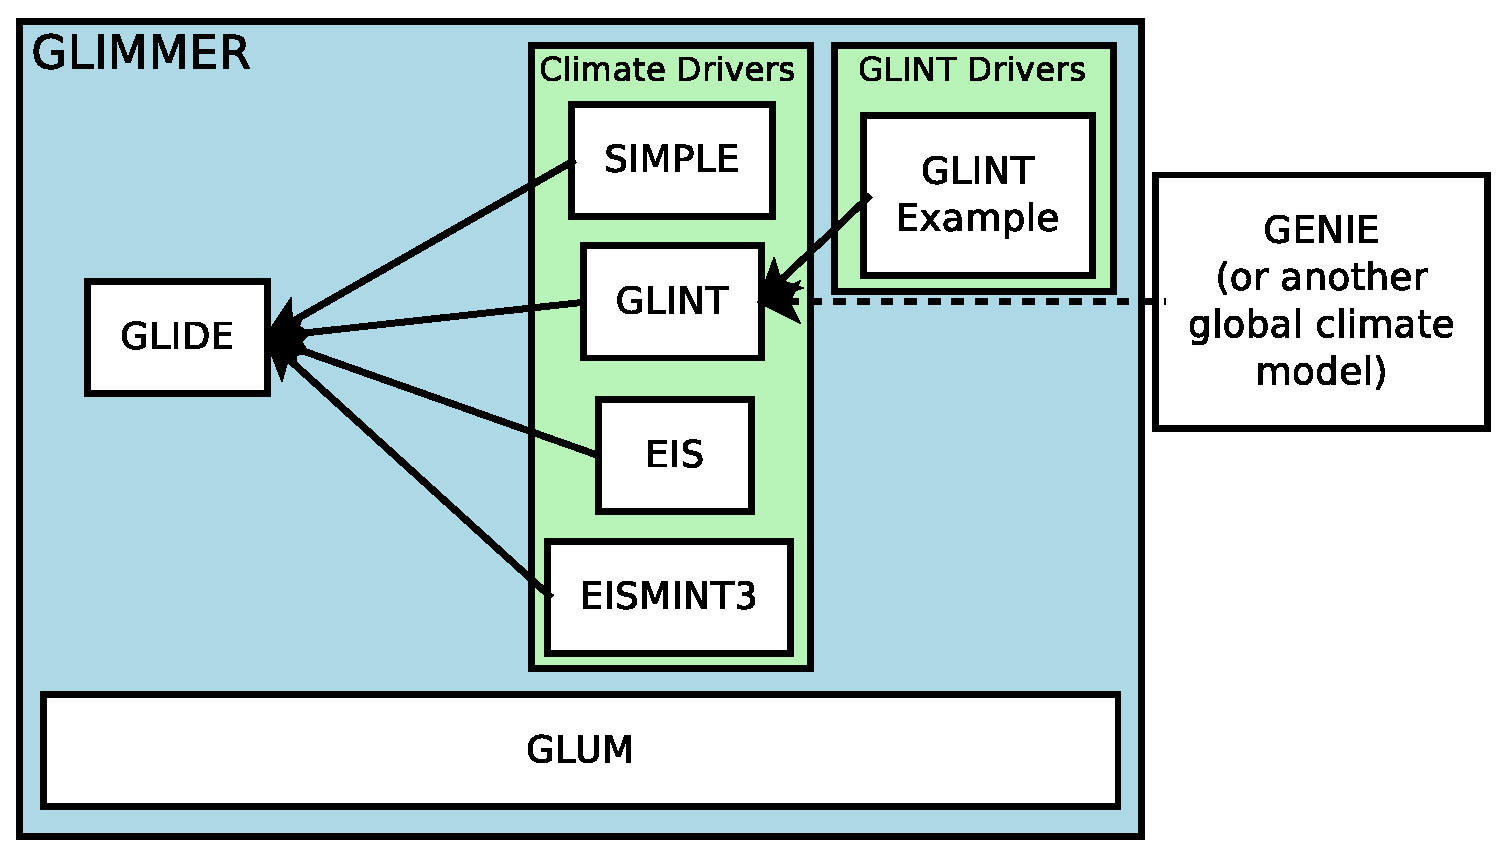
\includegraphics[width=0.6\textwidth]{\dir/figs/glimmer.eps}
%  \caption{Relationship between the various GLIMMER components.}
%  \label{ug.fig.glimmer}
%\end{figure}
%The relationship between the GLIMMER components is illustrated in Figure \ref{ug.fig.glimmer}.
%%
%\subsection{Climate Drivers}
%\label{subsec:climdrive}
%The core ice sheet model, GLIDE, is connected to the climate via the surface mass balance and temperature fields and (optionally) a scalar value for eustatic sea level. These drivers can be derived from simple assumptions, e.g. uniform mass balance or EISMINT tests, or from climate model output, e.g. GENIE or a regional climate model. These components, and how they relate to each other, are outlined in Figure \ref{ug.glide}.
%%
%\begin{figure}[htbp]
% \begin{center}
%   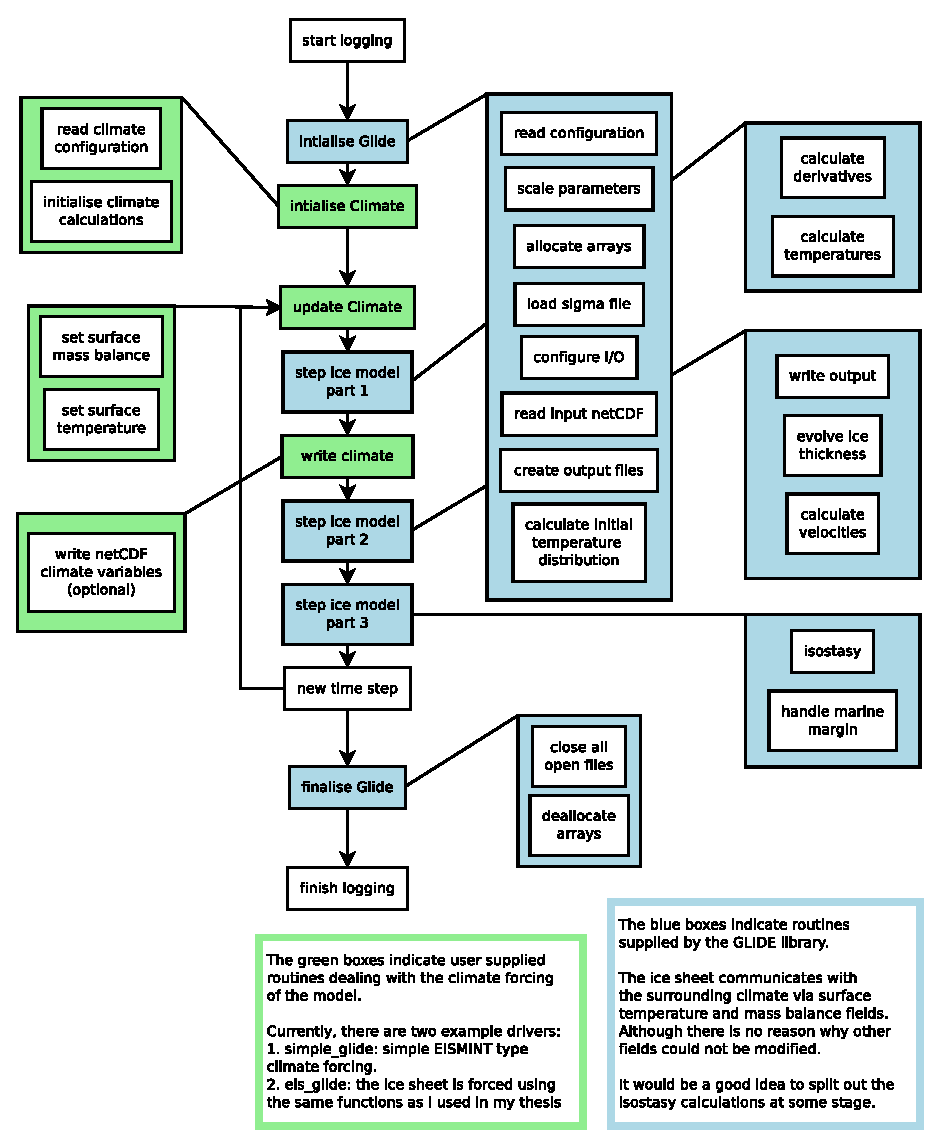
\includegraphics[width=0.9\textwidth]{\dir/figs/glide.eps}
% \end{center}
% \caption{Outline of the GLIDE and Climate components.}
%\label{ug.glide}
%\end{figure}
%%
%\subsection{Configuration, I/O and Visualisation}
%In general terms, each component is configured using a configuration file similar to Windows \texttt{.ini} files. At run-time, model configuration is printed to a log file. 
%
%2D and 3D data is read/written to/from netCDF files using the CF (Climate-Forecast) metadata convention\footnote{\texttt{http://www.cgd.ucar.edu/cms/eaton/cf-metadata/}}. NetCDF is a scientific data format for storing multidimensional data in a platform- and language-independent binary format. The CF conventions specify the metadata used to describe the file contents.
%
%Many programs can process and visualise netCDF data, e.g. OpenDX, Matlab, IDL, etc. Additionally, the GLIMMER code bundle contains GMT scripts written in Python to visualise the output.


\chapter{Installing GLIMMER-CISM}
\renewcommand{\dir}{install}

\section{Getting and Installing CISM}
\label{sec:getcode}

\href{http://oceans11.lanl.gov/cism/}{CISM}\footnote{\texttt{http://oceans11.lanl.gov/cism/}} 
is a relatively complex system of libraries and programs which build on other libraries. 
This section documents how to download and install CISM and its prerequisites.
Many common problems and questions can be addressed using the 
\href{http://forum.cgd.ucar.edu/forums/ice-sheet-modeling-cism}{user discussion boards}\footnote{\texttt{http://forum.cgd.ucar.edu/forums/ice-sheet-modeling-cism}}
. 
A CISM users mailing list is also available and can be subscribed to by sending an email
to \texttt{cism-users@googlegroups.com}\footnote{In order to subscribe from a non-Google email
address, you should first make sure to completely log out from any Google sites (e.g., Gmail) before sending 
your request. If you do not, it will automatically try to associate your request with your Gmail account instead.}.
Please report unresolved problems using the bug reporting facility at the 
\href{https://github.com/CISM/cism/issues}{CISM Github website}\footnote{\texttt{https://github.com/CISM/cism/issues}}. 

CISM is distributed as source code, and a reasonably complete build environment is therefore required to compile the model. 
For UNIX and LINUX based systems (including Mac), the \href{http://www.cmake.org/}{CMake} build system is used to build the model. 
Sample build scripts for a number of standard architectures are included, as are working build scripts 
for a number of large-scale, high-performance-computing architectures 
(e.g., \textit{Yellowstone} (CISL), \textit{Titan} (OLCF), and \textit{Hopper} (NERSC) ). 

There are two ways to get the source code:

\begin{enumerate}

\item \href{https://github.com/CISM/cism/releases}{Download}\footnote{\texttt{https://github.com/CISM/cism/releases}} a {\it released} version of the code as an archive (.zip or .tar.gz file).
\item Clone the code from the \href{https://github.com/CISM/cism}{CISM Github repository}\footnote{\texttt{https://github.com/CISM/cism}} using the following command: 
\texttt{git clone https://github.com/CISM/cism.git}
(It is also possible to clone the repository using the SSH protocol 
if you have an SSH keypair generated on your computer and attached to your GitHub account.  
See the \href{https://github.com/CISM/cism}{CISM Github repository webpage} and 
\href{https://help.github.com/articles/which-remote-url-should-i-use}{Github's help pages} for more information.)

\end{enumerate}

For beginners, downloading a zip archive of the latest release tag is recommended. 
More experienced users may want to download directly from the repository, 
as it will make updating the code easier in the future.

In either case, a Fortran90 compiler is required.  
Other software dependencies include the \href{http://www.unidata.ucar.edu/packages/netcdf/index.html}{netCDF} library 
(used for data I/O) and a \href{http://www.python.org}{Python} distribution 
(used to analyze dependencies and to automatically generate parts of the code) 
with a number of specific Python modules. Users who want to run the code in parallel will need to install MPI, 
and users who want access to the \textit{Trilinos} solver library will need to 
download and build \textit{Trilinos}, and link to it when building CISM. 
Finally, you will need CMake and Gnu Make to compile the code and link to the various third-party libraries. 

If you have not done so already, clone a tagged version of CISM or download an archive of the code, as noted above. Store the code or the unzipped/untarred archive in a location of your choice. More detailed build instructions, including instructions for the installation of supporting software, are given below.

% =====================================
% =====================================
\section{Installing Supporting Software for Basic (Serial) CISM}
% =====================================
% =====================================

Because the build process can be fairly complicated, we describe it in detail below, 
relying on the use of a package manager to handle many of the standard software dependencies. 
For each step we give specific instructions for both Mac OS X using MacPorts (in red boxes) and
Linux (in blue boxes). For the latter, we have verified that the instructions work for Ubuntu 12.10 and 14.04 LTS.
For different but related systems, hopefully these instructions can be used as a guide.

CISM can be installed in either a serial or parallel configuration. The parallel mode
allows the model to be run on multiple processors which can greatly speed up execution.
This is a common configuration to use on supercomputing clusters, but can also be 
convenient on modern desktops and laptops which often have four or more cores available.
However, the parallel build requires additional supporting software, so we first 
detail how to build serial CISM.  For new users, it is recommended to first build
and successfully run serial CISM before moving on to the parallel build.  

\textbf{Note:} Glide, the shallow-ice dycore, can only run on a single processor, 
even when the code is built with full parallel support. This is also true of the SLAP
solver routines.

The instructions below assume the user has administrative privileges for
installing new software (note the extensive use of \texttt{sudo}).  
If you are working on a shared machine without
administrative privileges, you might proceed by assuming all needed packages are present and 
continue to the CISM installation section.  If you encounter problems, you can refer back to this
section to determine which packages might be missing or
problematic before contacting your system administrator.


\begin{mdframed}[style=mac] % V==============MAC================V
As mentioned above, we will take advantage of \href{http://www.macports.org/}{MacPorts}, 
a software package manager for Macs. This will allow us to install most of 
the base level software libraries needed by CISM with few complications. 

Go to \href{http://www.macports.org/install.php}{http://www.macports.org/install.php}, where you will find a range of ".pkg" installs available, including those for Mountain Lion, Lion, and Mavericks versions of Mac OS X. 

Installing MacPorts requires installing the Xcode developer toolset provided by Apple. Details of how to obtain Xcode vary by version of OS X. See MacPorts installation instructions and this \href{https://developer.apple.com/xcode/downloads/}{link} for details. Once Xcode is installed, you may need to additionally download the ``command line tool'' from the Preferences / Downloads menu of Xcode. 

Depending on computer security settings at your institution (firewalls, etc.), 
you may need to add proxy information so that Macports can communicate and 
download software from the outside world. All Macports software will be installed 
under \texttt{/opt/local/} by default. To add proxy information, after installing 
Macports, edit the configuration file at \texttt{/opt/local/etc/macports/macports.conf}.
(Note this is probably a read-only file that requires superuser permission to edit,
so you will need to edit the file with something like: \texttt{sudo vim /opt/local/etc/macports/macports.conf}). 
By searching for the text string ``proxy'', you will find the lines like 
\texttt{proxy\_http hostname:12345} near the bottom of the file. Enter your proxy 
information here as appropriate (e.g., \texttt{hostname:your\_host\_info\_here}).

If you have previously installed Macports but not updated it recently, it's generally a good idea to do so. Ideally, this should be done with admin or root privileges (you will be prompted to enter your password) using:

\texttt{sudo port selfupdate}

\noindent
You will then be prompted to update any installed ports that are outdated, which you can do using:

\texttt{sudo port upgrade outdated}

\noindent
To search for available software in Macports, type: 

\texttt{port search software-name}

\noindent
Software is installed through Macports using the command:

\texttt{sudo port install software-name}

\noindent
Additional Macports tips will follow inline below. Extensive documentation for Macports 
can be found at the \href{http://guide.macports.org}{Macports} website.
\end{mdframed}              % ^==============MAC================^


\begin{mdframed}[style=ubuntu] % V==============UBUNTU==========V
This Ubuntu instructions describe setting up supporting software and CISM in a Linux environment.
These instructions were written using a fresh installation of Ubuntu 12.10 but 
steps should be very similar in other versions of Ubuntu or other distributions of Linux.
Instructions make use of the command line tool for installing packages that comes with Ubuntu, 
\texttt{apt-get}.  Other package management tools (e.g., Software Center)
could also be used.

\noindent

It's generally a good idea to synchronize your local package index files before
installing new software using \texttt{apt-get}:

\texttt{sudo apt-get update}

\noindent
To search for available packages, type:

\texttt{apt-cache search software-name}

\noindent
And to see detailed information about a package, type:

\texttt{apt-cache show software-name}

\noindent
Packages are installed through apt-get using the command:

\texttt{sudo apt-get install software-name}

\noindent
Some users have reported that BLAS and LAPACK libraries need to installed explicitly, for example when starting from a ``clean" machine. 
To do this, use the following two commands:

\texttt{sudo apt-get install libblas-dev}

\noindent
and

\texttt{sudo apt-get install liblapack-dev}

\noindent
Additional apt-get tips will follow inline below. Extensive documentation for apt-get 
can be found at the \href{https://help.ubuntu.com/community/AptGet/Howto}{Ubuntu} website
and through man pages (\texttt{man apt-get}).
\end{mdframed}                 % ^==============UBUNTU==========^



% =====================================
\subsection{Install git version control software}
% =====================================
If you intend to download the CISM code as a git repository, you will need the \texttt{git} package installed.
If you prefer to download a zipped archive of the code, this step can be skipped.


\begin{mdframed}[style=mac] % V==============MAC================V
Install git with:

\texttt{sudo port install git}
\end{mdframed}              % ^==============MAC================^


\begin{mdframed}[style=ubuntu] % V==============UBUNTU==========V
Install git with:

\texttt{sudo apt-get install git}
\end{mdframed}                 % ^==============UBUNTU==========^


% =====================================
\subsection{Install the GCC compiler suite}
% =====================================

The GCC compiler suite contains compilers for C, C++, and, optionally, Fortran.
Fortran and C compilers are required for serial CISM, and a C++ compiler is also
needed for parallel CISM.  CISM is known to work with GNU gfortran compilers, 
Intel ifort, and PGI.  In these instructions we will use GNU compilers because they
have been extensively tested with CISM and are freely available.  Advanced users
are welcome to use other compilers of their choosing.

CISM has been tested extensively with \texttt{gfortran} versions 4.5 and 4.6.
Newer (or older) versions may also work, although version 4.8 introduces 
new features that may uncover issues.

\begin{mdframed}[style=mac] % V==============MAC================V
Searching for gcc with \texttt{port search gcc} will return:

\begin{verbatim}
gcc44 @4.4.7 (lang) 
    The GNU compiler collection 
...
\end{verbatim}

in addition to a lot of other information on available Macports installs related to the GCC (Gnu) compiler suite. 

Where possible, we want to make sure that all other software we build and install 
with Macports uses the version of GCC we choose to install. To date, we've had success 
with GCC 4.6.3 (others may work as well but have not been tested). 
To install GCC 4.6.3 type:

\texttt{sudo port install gcc46}

You will see some verbose output telling you what is happening (downloading packages, 
expanding them, building, installing, checking, etc.). When the install is complete, you can type: 

\texttt{port installed} 

to see what packages you currently have installed. You should see 
something like \texttt{gcc46 \@4.6.3\_3 (active)}. 
(The minor version numbers after the ``4.6'' may differ as MacPorts makes updates to the port.) 
You will likely also see other packages that have been installed (software dependencies for GCC 
that were automatically installed by MacPorts and/or other ports you have manually installed). 

The ``(active)" description identifies which version of a particular package Macports 
currently thinks you want to use (e.g., you could also have another older GCC suite installed). 
To make sure the newly installed version is active, you would type:

\texttt{port select gcc}

which will return something like:

\begin{verbatim}
Available versions for gcc:
   gcc40
   gcc42
   mp-gcc46 (active)
   none
\end{verbatim}

This confirms that GCC 4.6 is active (the \texttt{mp} indicates a Macports version). 
It is possible that gcc46 will be listed as active when you type \texttt{port installed}, 
but that mp-gcc46 will not be listed as active when you type \texttt{port select gcc}. 
If mp-gcc46 is not active as shown above, then you will need to select it using:

\begin{verbatim}
	sudo port select --set gcc mp-gcc46
\end{verbatim}

This will ensure that any generic call to gcc, gfortran, g++, will point to the libraries just installed.

\end{mdframed}              % ^==============MAC================^


\begin{mdframed}[style=ubuntu] % V==============UBUNTU==========V
GNU compilers may have come with your Linux distribution.  If not, they need to 
installed.  Ubuntu 12.10 comes with \texttt{gcc} installed but not \texttt{gfortran}.

Install \texttt{gfortran} with:

\texttt{sudo apt-get install gfortran}

\end{mdframed}                 % ^==============UBUNTU==========^


% =====================================
\subsection{Install build tools}
% =====================================

Additional tools are needed for managing the build process.  \texttt{make} (specifically, GNU's gmake)
usually comes with Mac and Linux distributions, but if not it should be installed.  
Additionally, CISM uses the \href{http://www.cmake.org/}{\texttt{CMake} build utility}
(a cross-platform, open-source build system).

\begin{mdframed}[style=mac] % V==============MAC================V

While you probably already have a version of \texttt{make} on your system, it may be out of date or conflict with other Macports installed software. The required versions for CISM can be installed through Macports with this command: 

\begin{verbatim}
sudo port install gmake cake
\end{verbatim}

In addition to the software installed above, you should now see something like the following when you type \texttt{port installed}:

\begin{verbatim}
  gmake @3.82_0 (active)
  cmake @2.8.10_1 (active)
\end{verbatim}
\end{mdframed}              % ^==============MAC================^



\begin{mdframed}[style=ubuntu] % V==============UBUNTU==========V

On Ubuntu (and other Debian systems) there is usually a package called \texttt{build-essential} 
that includes a large collection of tools and libraries that are typically necessary
for compiling code. Install these tools and \texttt{CMake} with:

\texttt{sudo apt-get install build-essential cmake cmake-curses-gui}
\end{mdframed}                 % ^==============UBUNTU==========^


% =====================================
\subsection{Install netCDF}
% =====================================
\label{sec:install-netcdf}
NetCDF stands for ``network Common Data Form'' libraries, which are a
 machine-independent format for representing scientific data.
This is required by CISM for performing input/output.  The netCDF package you 
install must include Fortran libraries for CISM to compile (in some package managers,
the Fortran libraries are in a separate package).  There are substantial differences 
between versions 3.x and 4.x of netCDF, but both version series should work with CISM. 
It is also possible to download and compile netCDF libraries manually, 
which may be preferred by advanced users wanting to use a specific version.

It is also recommended that you install optional tools for working with netCDF datafiles.
\href{http://meteora.ucsd.edu/~pierce/ncview_home_page.html}{\texttt{ncview}} is a
convenient tools for viewing netCDF files.  
(Some alternatives are to write Python or Matlab scripts or to use another tool like Paraview or
\href{http://ferret.pmel.noaa.gov/Ferret/home}{\texttt{Ferret}}.)  
\href{http://nco.sourceforge.net/}{\texttt{NCO}} (``netCDF Operators'') is a toolkit of command line tools
for manipulating and analyzing data stored in netCDF-accessible formats.

\begin{mdframed}[style=mac] % V==============MAC================V
To install NetCDF, use \texttt{sudo port install netcdf-fortran +gcc46}. 
Note that there are other versions of NetCDF available to install. It is important 
to choose the one with the ``Fortran" extension. The ``gcc46" syntax specifies a port ``variant". 
This tell Macports that, if there is a version of the selected software 
to install that is consistent with the GCC 4.6 compiler suite, then it should 
choose that one. Typing \texttt{port installed} should now include:

\begin{verbatim}
netcdf @4.3.2_0+dap+gcc46+netcdf4 (active)
netcdf-fortran @4.2_12+gcc46 (active)
\end{verbatim}

The ``dap+gcc46+netcdf4" comes along automatically. 

\textbf{Optional but recommended:} Tools for working with netCDF data files.

\texttt{sudo port install ncview nco}

If you encounter an `unable to open display' error when running \texttt{ncview},
you may need to install a newer version of the X Window System than the one provided by Apple.
We have had success using the latest version of XQuartz:
\href{http://xquartz.macosforge.org}{http://xquartz.macosforge.org}

\end{mdframed}              % ^==============MAC================^


\begin{mdframed}[style=ubuntu] % V==============UBUNTU==========V
Install netCDF libraries with:

\texttt{sudo apt-get install libnetcdf-dev}

\textbf{Optional but recommended:} Tools for working with netCDF data files.

\texttt{sudo apt-get install netcdf-bin ncview nco}
\end{mdframed}                 % ^==============UBUNTU==========^



% =====================================
\subsection{Install Python and related modules}
% =====================================
Python is used by CISM to autogenerate I/O code during compilation, and is also
used by most test case scripts to set up initial conditions and analyze and plot
results.  Only Python 2.7 has been tested.  Python 3 may work for some uses but is
likely to generate errors due to extensive changes between versions 2 and 3.
Also, CISM uses a number of python modules:
\begin{itemize}
  \item \texttt{numpy} - required for generating many test case initial conditions
  \item \texttt{matplotlib} - used by some plotting scripts.  Not strictly necessary but required for those scripts to work properly.
  \item  a python netCDF I/O module.  Options are \texttt{netCDF4},  \texttt{Scientific.IO.NetCDF}, or \texttt{PyCDF}.  
\texttt{netCDF4} is the ideal choice, but it is often not available through Linux package managers and must be installed through a python package manager like pip, or manually.
\texttt{PyCDF} is the least recommended option here because it is not entirely compatible with the others.  \texttt{Scientific.IO.NetCDF} is usually available through Linux package managers.
\end{itemize}


\begin{mdframed}[style=mac] % V==============MAC================V
While Mac OS X already comes with a working Python distribution, we will need 
additional modules that can sometimes be tricky to get working together correctly. 
We have successfully used both the 
\href{https://www.enthought.com/products/epd/}{Enthought Python distribution} 
(which is free for people associated with a university) and a version installed 
using Macports.  To obtain and install Enthought, click on the link above and follow their directions.
To install version 2.7 using Macports, along with the necessary 
additional modules, do the following:

\texttt{sudo port install python27 py27-numpy py27-matplotlib py27-scientific}

\texttt{          py27-netcdf4}

The existence of two versions of python on your system can lead to confusion.
It is important that you leave the version of python that came supplied by Apple so that
your system has access to it.  However, you will want to be sure that CISM has access to
the new, more modern version of python you have installed.  In our experience,
this can be one of the most problematic parts of the installation process.  
You can use \texttt{port select}:

\texttt{ sudo port select python python27}

\noindent
You can check that Macports python is used by default by typing:

\texttt{which python}

\noindent
and you should see: \texttt{/opt/local/bin/python}.  
If you instead see \texttt{/usr/bin/python} then the default Apple python is still 
the version that is being used on the command line.  If this happens, or if you 
encounter errors with this setup, an alternative approach is to modify the 
\texttt{PATH} variable in your \texttt{.bashrc} or similar environment settings script
to make sure that \texttt{/opt/local/bin} is before \texttt{/usr/bin} in your path.
\end{mdframed}              % ^==============MAC================^



\begin{mdframed}[style=ubuntu] % V==============UBUNTU==========V
Python generally comes with most Linux distributions.  If it is not present, it must be installed.
Often, there is an additional python development package that is necessary
when working with compiled code (tpyically called \texttt{python-dev} on Ubuntu).

Install python modules with:

\texttt{sudo apt-get install python-dev python-numpy python-matplotlib} 

\texttt{          python-scientific}

\textbf{Optional:} Installing \texttt{netCDF4} python module.

\noindent
Install pip (a tool for installing and managing Python packages):

\texttt{sudo apt-get install pip}\footnote{For Ubuntu 14.04 there is a known issue with pip and handling freetypes. This can be fixed using \texttt{sudo apt-get install libfreetype6-dev libxft-dev}.}

\noindent
%Install \texttt{netCDF4} using pip:
Next, install \texttt{HDF5} using pip:

\texttt{sudo apt-get install libhdf5-dev hdf5-tools hdf5-helpers flex}

\noindent
Finally, install \texttt{netCDF4} using pip:

\texttt{sudo -E pip install netcdf4}
\end{mdframed}                 % ^==============UBUNTU==========^



% =====================================
% =====================================
\section{Building Serial CISM}
\label{serial-build}
% =====================================
% =====================================
At this point we are ready to build a \textit{serial} version of CISM and its linked libraries. While we ultimately want to build a 
version of the code that also runs in parallel, it is often useful to stop at this step to make sure everything is working. Then, if 
problems occur during the parallel build process (as they sometimes do), we know those problems have occurred only during 
the last step of the process.

If you have not already done so, obtain the source code following the instructions above in section \ref{sec:getcode}. Below, all 
paths starting with \texttt{./} indicate the root level of the source code directory. E.g., if you expanded your tar.gz archive into a main source code 
directory with the path \texttt{/usr/JohnDoe/CISM}, the \texttt{./} refers to the path \texttt{/usr/JohnDoe/CISM/}.  

Unlike previous versions of the code, the build system is now entirely based on CMake 
(Autotools is no longer used). 

Build scripts are provided that should work for most standard Mac and Linux setups, 
as well as some supercomputing platforms on which CISM is commonly run.
All build scripts are located in the \texttt{./builds} directory from the root level of the code.
In general, change to the subdirectory that most closely matches your system and intended
build.

If you encounter an error when using the included scripts, you may need to modify some details, 
such as the location of your NetCDF libraries or your compiler names.  Other errors you might 
encounter may indicate that some of the supporting software (above) is missing.

%\textbf{SP: For the cake build to ''just work" (i.e., w/o setting an env vars, etc.), the only thing I had to do was to sym link the generic compiler names (e.g. gcc, g++, gfortran) and python in /opt/local/bin/ to the respective binary files there w/ a specific name (e.g., gcc-mp-6.4). Assuming one is in /opt/local/bin/, an example of that would be 'sudo ln -s ./gfortran-mp-4.6 ./gfortran'. This also assumes, that ones path has been pre-prended to look in /opt/local/ first, rather then /usr/local. This should have happened automatically when installing macports (it adds a line to your .profile script to cover this), but it might be worth mentioning explicitly (at the start?) as well. Note that after the fact, I found out that a more general / easier way of doing this might be to instead do, e.g., 'sudo port select --set gcc gcc46'. I have not tested this, but it is recommended (and seemed to work) for using of openmpi, e.g. by way of slaving the generic "mpi" to "openmpi-devel-gcc46-fortran". This is a faster way to do it, as it sets all the necessary sym links with a single command. I've already changed the gcc documentation above to reflect this. It would be good for someone else to confirm this if / when they do a clean install on a new machine.} 

\begin{mdframed}[style=mac] % V==============MAC================V
On a Mac, you should be able to build the code by doing the following:

\begin{enumerate}
\item{Change to the \texttt{./builds/mac-gnu} directory from the root level of the code.}
\item{Configure the build using \texttt{source mac-gnu-serial-cmake}}
\item{Build the code using \texttt{make -j X}, where the ``X'' refers to the number of processors available for use in the build (or just \texttt{make} if you have only one processor).}
\end{enumerate}
\end{mdframed}              % ^==============MAC================^


\begin{mdframed}[style=ubuntu] % V==============UBUNTU==========V
On a Linux platform, you should be able to build the code by doing the following:

\begin{enumerate}
\item{Change to the \texttt{./builds/linux-gnu} directory from the root level of the code.}
\item{Configure the build using \texttt{source linux-gnu-serial-cmake}}
\item{Build the code using \texttt{make -j X}, where the ``X'' refers to the number of processors available for use in the build (or just \texttt{make} if you have only one processor).}
\end{enumerate}
\end{mdframed}                 % ^==============UBUNTU==========^

When the build completes, you can check for the executable driver by typing \texttt{ls cism\_driver} from within the current build directory (here, from within the \texttt{./builds/mac-gnu} or \texttt{./builds/linux-gnu/} directory). The file \texttt{cism\_driver} is the executable you will link to when running the model, which is generally done using a symbolic link. For example, from the \texttt{./tests/higher-order/shelf/} directory, one would link to this executable using, 

\begin{verbatim}
ln -s ../../../builds/mac-gnu/cism_driver/cism_driver ./
\end{verbatim}

Chapter \ref{ch:tests} discusses running the executable for standard test cases.

Advanced users may want more control over the build scripts.  There are a number of
build options used by CMake to customize the build.  You can manually modify the 
build scripts included with the code, or use the tool \texttt{ccmake} to 
interactively adjust build options (type \texttt{ccmake ../../} from any build directory
after having run the configure script once).  The available options are listed in Table \ref{cmake-options}.
Many of these options pertain to the parallel build which is discussed in more detail below.


\begin{table}
\begin{tabular}{ l | p{8cm} }
\hline
\texttt{CISM\_BUILD\_CISM\_DRIVER} & Toggle to build cism\_driver, on by default \\

\texttt{CISM\_BUILD\_EXTRA\_EXECUTABLES} & Toggle to build other executables, off by default \\

%\texttt{CISM\_BUILD\_SIMPLE\_GLIDE} &  Toggle to build simple\_glide, on by default \\

\texttt{CISM\_COUPLED} & Toggle to build CISM for use with CESM, off by default \\

\texttt{CISM\_ENABLE\_BISICLES} & Toggle to build a BISICLES-capable cism\_driver, off by default  \\

\texttt{CISM\_FORCE\_FORTRAN\_LINKER} & Toggle to force using a Fortran linker for building executables, off by default \\

\texttt{CISM\_GNU} & Toggle to set compilation flags needed for the gnu compiler, off by default \\

\texttt{CISM\_INCLUDE\_IMPLICIT\_LINK\_LIB} & Toggle to explicitly include the CMAKE\_Fortran\_IMPLICIT\_LINK\_LIBRARIES on the link line, on by default \\

\texttt{CISM\_MPI\_MODE} & Toggle to configure with MPI, on by default \\

\texttt{CISM\_NETCDF\_LIBS} &  netCDF library name(s) \\

\texttt{CISM\_NO\_EXECUTABLE} & Set to  ON  to just build libraries, off by default \\

\texttt{CISM\_SERIAL\_MODE} & Toggle to configure in serial mode: off by default \\

\texttt{CISM\_SOURCEMOD\_DIR} &  Path to SourceMod directory of F90 files to replace CISM files \\

\texttt{CISM\_STATIC\_LINKING} &  Toggle to set static linking for executables, off by default \\

\texttt{CISM\_USE\_DEFAULT\_IO} &  Toggle to use default i/o files rather than running python script, off by default \\

\texttt{CISM\_USE\_GPTL\_INSTRUMENTATION} & Toggle to use GPTL instrumentation, on by default \\

\texttt{CISM\_USE\_MPI\_WITH\_SLAP} & Toggle to use mpi when using SLAP solver, only relevant if CISM\_SERIAL\_MODE=ON, off by default \\

\texttt{CISM\_USE\_TRILINOS} & Toggle to use Trilinos external solver libraries, on by default \\

\texttt{CMAKE\_VERBOSE\_CONFIGURE} & Verbose CMake configuration, on by default \\

%% older options below here %%

%\texttt{CISM\_USE\_CISM\_FRONT\_END} &  Toggle to use cism\_driver or cism\_cesm\_interface with cism\_front\_end, off by default \\

%\texttt{CISM\_BUILD\_GLINT} & Toggle to build glint, off by default \\

%\texttt{CISM\_BUILD\_GLINT\_EXAMPLE} & Toggle to build glint\_example, off by default \\

%% some probably not important options here %%

%\texttt{CISM\_NETCDFF\_FOUND} & Path to NetCDF libraries  \textbf{** do we need to include this here? **} \\                                                                                                                        

\hline
\end{tabular}
  \caption{Available \texttt{CMake} settings for configuring the CISM build process}
  \label{cmake-options}
\end{table}

Also, there are standard CMake options that can be set (e.g., \texttt{CMAKE\_C\_COMPILER}, \texttt{CMAKE\_Fortran\_COMPILER}, etc.).  Many of these are explained in the \href{http://www.cmake.org/Wiki/CMake_Useful_Variables}{CMake documentation}.



% =====================================
% =====================================
\section{Installing Supporting Software for Parallel CISM}
% =====================================
% =====================================
To build parallel CISM, MPI compilers and libraries are required.  
Only the higher-order dycore (Glissade) can run in parallel.  (There is also a
higher-order dycore called Glam that can be run in parallel, but it is used
for development and testing and is not supported for scientific applications.)

In addition, you may choose to include the Trilinos package of external solver libraries.  
These are not required, but for some problems Trilinos may provide better
performance and stability than the native solvers.  Trilinos can also technically be 
used with a serial build, but this configuration is not supported or recommended.

% =====================================
\subsection{Install MPI}
% =====================================
MPI (Message Passing Interface) libraries and compilers are necessary for compiling parallel CISM.  
These libraries are used for handling parallel communications when running the 
code on multiple processors. A more complete description of parallel 
model configurations is given in Chapter \ref{ch:runcism}. 
(For example, some test cases and configurations when running the shallow-ice 
dycore are not fully supported in parallel). 
OpenMPI and MPICH are two common MPI implementations.

\begin{mdframed}[style=mac] % V==============MAC================V
It is likely that you already have versions of MPI installed on your system, 
but they may be out of date or not compatible with the other libraries we have 
and will be installing. Using Macports, the MPICH version of MPI is known 
to work when building CISM.  (OpenMPI may also work, but we've seen more 
consistent success on Macs with MPICH.)

First, check Macports for available versions of MPICH using \texttt{port search mpich*}. We want 
the version that is compatible with our GCC compiler suite, so we type: 

\begin{verbatim}
	sudo port install mpich-devel-gcc46 +fortran
\end{verbatim}

\noindent
To make sure this is active, type 
\begin{verbatim}
	port installed mpi*
\end{verbatim}

\noindent
which should return

\begin{verbatim}
     mpich-devel-gcc46 @3.2a1_0+fortran (active)
\end{verbatim}

\noindent
As when installing the GCC compilers, we want to make sure any generic call to MPI points to MPICH. This 
can be done with the following command:

\begin{verbatim}
	sudo port select --set mpi mpich-devel-gcc46-fortran
\end{verbatim}

\end{mdframed}              % ^==============MAC================^



\begin{mdframed}[style=ubuntu] % V==============UBUNTU==========V
Either OpenMPI or MPICH are likely to work with CISM on Linux machines.
On Linux machines, we have tested OpenMPI more thoroughly.
Install OpenMPI with:

\texttt{sudo apt-get install openmpi-bin}
\end{mdframed}                 % ^==============UBUNTU==========^



% =====================================
\subsection{Install Trilinos solver libraries}
\label{sc:install_trilinos}
% =====================================

Trilinos is a modern, open source, C++ based library of parallel nonlinear and linear solvers, 
preconditioning and mesh-partitioning tools, and much more. It can be downloaded 
\href{http://trilinos.org/download/}{here}\footnote{http://trilinos.org/download/}.
(The software is free, but you are required to enter your email address to download it.) 
The documentation below assumes that you are working with version 11.10.* and was specifically 
tested using version 11.10.2. 

Building Trilinos requires CMake version 2.8 or later, which ideally you have already 
installed as discussed above. Trilinos is not needed to run the default 
parallel, higher-order dycore (Glissade), but it may be useful for  
more difficult problems or for debugging in cases where the native Fortran solvers 
fail to converge.

The build instructions for Trilinos on Mac and Linux are very similar, so users
of both systems can follow the primary instructions below, except where noted.

Trilinos requires both (1) an ``out-of-source build'' and (2) an ``out-of-build installation''. 
This means that you cannot build the code in the same directory where the source code lives, 
and you cannot install the libraries in the same directory where you build the code.
(Older versions of Trilinos required an out-of-source build but not an out-of-build installation.) 
The easiest way to satisfy this requirement is to have separate ``source'', ``build'' and 
``install'' directories in the location where you want to install the code. 
For example, in \texttt{/usr/local/}, you could set up the following three directories:

\begin{verbatim}
	trilinos-11.10.2-Source/
	trilinos-11.10.2-Build/
	trilinos-11.10.2-Install/
\end{verbatim}

The ``source'' directory will be created on its own when you uncompress the tar.gz archive 
that you download. You do not have to keep the source code where you build and install 
the Trilinos libraries, but you will need to remember the path to where that source code 
lives on your computer. 

To configure the Trilinos build, you will need to execute a CMake configure script. 
Sample configure scripts for a number of standard platforms are included in the ``sampleScripts''
directory under the root level of the Trilinos source code. 
Also, the CISM code includes examples of Trilinos configure scripts (``do-configure'') 
for use with CISM for both Linux and Mac platforms in the 
\texttt{./utils/trilinos\_config\_scripts\_examples} directory. 
We recommend starting with one of those scripts and modifying it as
necessary to work on your system\footnote{If you are following the above installation instructions for
Mac exactly, then the configure script 
\texttt{./utils/trilinos\_config\_scripts\_examples/do-configure-Trilinos-11.10.2-for-Mac-10.9.4} should 
work with few modifications.}.

The paths to both the ``source'' and ``install'' directories are specified within the ``do-configure'' scripts. In these instructions, those directories are both assumed to live within \texttt{/usr/local/},
but other locations are fine to use too (e.g., in your home/User directory).

\begin{mdframed}[style=mac] % V==============MAC================V
Also note the explicit path in the MPI lines, e.g.,

\begin{verbatim}
-D MPI_EXEC="/opt/local/mpiexec" \
\end{verbatim}

Since some Macs may come with their own pre-installed OpenMPI libraries, it is important here to specify the path to the version we previously installed using Macports.
\end{mdframed}              % ^==============MAC================^

Find the example script most appropriate for your system, copy it to the \texttt{trilinos-11.10.2-Build} directory, and modify it if necessary (e.g., adjust paths, compiler locations, etc.).
Execute it with: 

\texttt{source ./do-cmake}\footnote{Here we have assumed that the name of the configure script is ``do-cmake''. The script name may differ depending on what you have called it or if you copied and modified one of the scripts from \texttt{./utils/trilinos\_config\_scripts\_examples}.}

\noindent
from within your \texttt{trilinos-11.10.2-Build} directory. Depending on where you are building and installing the code, you may need to have administrative privileges (in which case you would type \texttt{sudo source ./do-cmake}). If the configure step was successful, you should see the following displayed on your screen:

\begin{verbatim}
...
Processing enabled package: [PACKAGE NAME]
...

Exporting library dependencies ...

Finished configuring Trilinos!

-- Configuring done
-- Generating done
-- Build files have been written to: /usr/local/trilinos-11.10.2-Build
\end{verbatim}

It is a good idea to scan the output while the ``do-cmake'' script is executing, 
for example to ensure the configure process is picking up the compilers you specified 
(e.g., it is using the Macports versions as opposed to some Mac default versions that 
might also be on your system). Once the code is configured successfully, build the libraries 
from within the \texttt{trilinos-11.10.2-Build} directory by typing:

\texttt{make} (or \texttt{sudo make} if necessary) 

\noindent
For multiprocessor machines, the build process can be sped up significantly using 
the ``-j''command as described above for building serial CISM:

\texttt{make -j X}

\noindent
where ``X'' is the number of cores available on your machine (e.g., \texttt{make -j 4} 
for a 2-processor, dual-core machine).

Building Trilinos can take a long time (e.g., an hour or more), depending on your machine, 
the number of processors used for the build, and the number and type of libraries 
you are installing. Once you have built the code, we highly recommend testing it 
using:

 \texttt{make test} 

\noindent
(The \texttt{Trilinos\_ENABLE\_TESTS:BOOL}
variable in the do-cmake script can be set to ``OFF''to disable building of the tests.)
Screen output will tell you if and how many tests failed. We have seen 
a few tests fail while still having a perfectly good and working Trilinos library. 
In general, if the number of tests passed is above 90\%, the library will likely work fine with CISM.
Query the CISM \href{mailto:cism-users+subscribe@googlegroups.com}{users} or
\href{mailto:cism-devel+subscribe@googlegroups.com}{developers} lists\footnote{cism-users+subscribe@googlegroups.com -or- cism-devel+subscribe@googlegroups.com} 
if you have questions about specific Trilinos tests failing.

\begin{mdframed}[style=mac] % V==============MAC================V
On a Mac, MPI tests have been known to trigger a dialog box from the firewall. 
With more than 300 tests, these messages popping up continually can make it impossible 
to use your computer until the tests complete. To keep them from appearing, you can temporarily 
turn off your firewall under ``System Preferences'' (Security $>$ Firewall $>$ Stop). 
Be sure to turn the firewall back on when the tests are complete!
\end{mdframed}              % ^==============MAC================^

After running the tests, you will need to install Trilinos using:

 \texttt{make install}

\noindent
This will build the actual Trilinos libraries in the path specified in the

\begin{verbatim}
-D CMAKE_INSTALL_PREFIX:PATH=/path
\end{verbatim} 

\noindent
line of your ``do-cmake'' script (above). For this example, those libraries will be 
installed in: \texttt{/usr/local/trilinos-11.10.2-Install}

After successfully building Trilinos, create an environment variable called \texttt{CISM\_TRILINOS\_DIR}
so the CISM build process can find the Trilinos installation.  For example, if you 
are using the bash shell and your current directory is the Trilinos install directory, you can do:
\begin{verbatim}
export CISM_TRILINOS_DIR=$PWD
\end{verbatim}
You may prefer to modify your .bashrc or .bash\_profile (or similar)
to set this environment variable on every login.

Alternatively, you can modify the CISM parallel build script (below) so that the line:
\begin{verbatim}
-D CISM_TRILINOS_DIR=$CISM_TRILINOS_DIR \
\end{verbatim}
is set to the Trilinos installation directory.





% =====================================
% =====================================
\section{Building Parallel CISM}
% =====================================
% =====================================

The procedure for building parallel CISM is nearly identical to the serial build (above).
The build script for parallel CISM for a Mac is located at \texttt{builds/mac-gnu/mac-gnu-cmake}, 
while the build script for Linux is located at \texttt{builds/linux-gnu/linux-gnu-cmake}.
From the appropriate directory, run:

\texttt{ source mac-gnu-cmake} or \texttt{ source linux-gnu-cmake}

\noindent{Once the configuration step completes successfully, you can compile the code as before with:}

\texttt{make}

\noindent{or}

\texttt{make -j 4}

\noindent{if you have 4 processors available (or as many processors as you would like to use).
See Section \ref{serial-build} for details about customizing the build process.

Building a parallel version of CISM that includes Trilinos requires setting the  
\begin{verbatim}
-D CISM_USE_TRILINOS 
\end{verbatim}
\noindent{flag to \texttt{ON} in the \texttt{builds/mac-gnu/mac-gnu-cmake} script.}

% =====================================
% =====================================
\section{Next Steps}
% =====================================
% =====================================
If you make any changes to the source code, you only need to re-run
\texttt{make} from your build directory to generate an updated executable.  
One exception is that if you edit the lists of input/output netCDF variables in 
\texttt{*\_vars.def} files (see Appendices \ref{ug.sec.varlist} and \ref{ch:appendix_io}), 
you need to first re-source the configuration script 
(e.g., \texttt{source mac-gnu-cmake}) before re-running \texttt{make}.


Now that you have successfully built the code, you can proceed to Chapters \ref{ch:modelingintro} and \ref{ch:higher-order} to learn more detailed 
information about ice sheet modeling, to Chapters \ref{ch:glide} and \ref{ch:glissade} to learn more about the various model approximations 
available through CISM, or you can proceed to Chapter \ref{ch:tests} to learn how to run and examine some standard model test cases.  





\chapter{Introduction to Ice Sheet Modeling}
\renewcommand{\dir}{modeling-intro}

In this chapter we give an introduction to ice dynamics and the governing conservation equations.

Ice sheets are key components of Earth's climate system. They contain
nearly all of the planet's fresh water, changes in their volume have an
immediate effect on sea level, changes in their area and surface
characteristics affect global albedo, and they play a role in the
circulation of both the atmosphere and the ocean. Through the latter
half of the Quaternary, ice sheets have modulated the planetary response
to orbitally-driven insolation cycles. Looking forward, the Greenland
and Antarctic ice sheets have the potential to play important roles in
climate change.

A numerical model is a discrete approximation of a continuous process.
The approximation is discrete due to the finite nature of a computer's
precision. The underlying process is continuous because it is commonly
formulated in terms of partial or ordinary differential equations.
Numerical models can not be solved until the boundary conditions and
initial conditions are specified. Such models may be very simple such as
a \href{Wikipedia:Harmonic oscillator}{Wikipedia:Harmonic oscillator},
or very complex, as in a
\href{Wikipedia:Global climate model}{Wikipedia:Global climate model}.

The model we will use is called CISM. It has its basis in a set of
programs and climate ``drivers'' built over many years by a research
group at the \href{http://www.bris.ac.uk/}{University of Bristol}, led
by Tony Payne. Historically, the effort was called
\href{http://forge.nesc.ac.uk/projects/glimmer/}{Glimmer}. More
recently, a collaborative project has extended the effort in many novel
and exciting ways. This is called the Community Ice Sheet Model, or
\href{http://websrv.cs.umt.edu/isis/}{CISM}.



% ========================================
\subsection{Conservation equations}

The mathematical descriptions of physical systems we encounter in Earth
science problems begin from statements requiring the conservation of
energy, momentum, or mass.

% ========================================
\subsubsection{Integral form}

The mathematical formulation of conservation can be arrived at by
considering the change in a quantity $\phi$ that is known in a
\textbf{control} volume $V$. The
\href{Wikipedia:control volume}{Wikipedia:control volume} is enclosed by
a surface $S$, with outward positive unit vector $\hat n$ normal to $S$.


\begin{figure}
  \begin{center}
    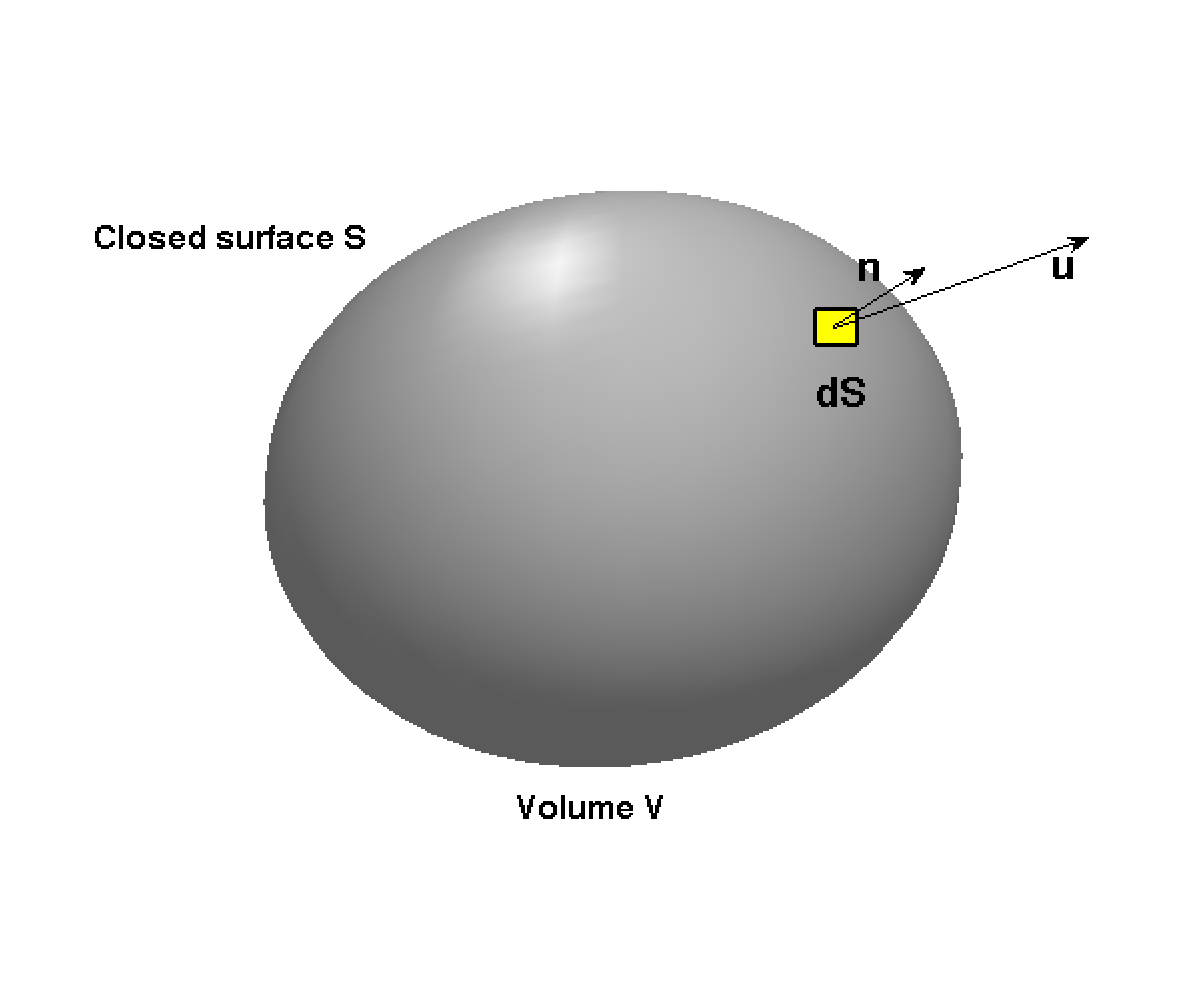
\includegraphics[width=0.9\columnwidth]{\dir/figs/ControlVolume.eps}
  \end{center}
  \caption{Diagram of control volume and associated quantities.}
  \label{fig:controlvol}
\end{figure} 


The value of $\phi$ within $V$ may change over time if

\begin{enumerate}
\itemsep1pt\parskip0pt\parsep0pt
\item
  there is a flux through $S$. The flux is partitioned into two parts,
  one due to \url{Wikipedia:diffusion} and another due to
  \url{Wikipedia:advection}.
\item
  Creation or destruction of $\phi$ within $V$.
\end{enumerate}

Formally, time rate of change in $\phi$ within $V$ is written:

$
{\frac{ \partial }{ \partial t}} { \int }_{ V} \phi dV~ = ~ -{ \int }_{ S} {\mathbf F}
    {\cdot} \hat n~ dS~ - ~{ \int }_{ S} \phi {\mathbf u} {\cdot} \hat n ~ dS~
    + ~{ \int }_{ V} HdV
$

where ${\mathbf F}$ represents the flux due to diffusion
($\mathbf{F} \propto \nabla \phi$), $\phi {\mathbf u}$ represents
velocity field \emph{\href{Wikipedia:advection}{advecting}} $\phi$, $H$
represents a source (or sink) of $\phi$. Vector quantities are
represented in \textbf{boldface}. The negative signs in front of the
first two terms on the right-hand side indicate that an outward flux
results in decrease of $\phi$ in the volume enclosed by $S$.

This statement of conservation of $\phi$ in the unit volume $V$ is
always true, independent of the size of $V$ and even if the fields
enclosed by $S$ are not continuous. This is the case because we
integrate over $V$. It is important to note that that information on
spatial scales smaller than $V$ is lost in the integration.

% ========================================
\subsubsection{Derivative form}

Numerical models are often easier to formulate from the derivative form
of the conservation equation. This requires the derivatives of $\phi$ to
exist within $V$. This requirement allows the integral form of the
conservation equation to be written as partial differential equations
which are upheld with in the control volume.

Begin with the terms describing diffusive and advective fluxes into or
out of the control volume. The
\href{Wikipedia:divergence theorem}{Wikipedia:divergence theorem} states
that

$
{ \int }_{S} {\mathbf F} {\cdot} \hat{n} ~dS~ = ~{ \int }_{V} \nabla 
    {\cdot} {\mathbf F} ~dV. 
$

Or, adapting the notation that the subscript indicates a single
component of a vector, and that repeated subscript indices in a single
term are to be summed,

$
{ \int }_{ S} {\mathbf F}_{ j} ~n_{ j} ~dS~ = ~{ \int }_{ V} {\frac{
    \partial {\mathbf F}_{ j} }{ \partial x_{ j} }} ~dV.
$

Using the divergence theorem, the surface integrals over fluxes may be
replaced,

$
-{ \int }_{ S} {\mathbf F} {\cdot} \hat{n}dS~ - ~{ \int }_{ S} \phi {\mathbf u}
    {\cdot}\hat{n} dS~ = ~ -{ \int }_{ V} \nabla {\cdot} \left ( {
    {\mathbf F}~ + ~ \phi ~ {\mathbf u}} \right )dV.
$

Assuming that the coordinate system is stationary with respect to the
velocity field $\mathbf{u}$ (Eularian reference frame), it is possible
to write

$
{\frac{ \partial}{ \partial t}} { \int }_{ V} \phi ~dV~ = ~{ \int }_{ V}
    {\frac{ \partial \phi }{ \partial t}} ~dV~
$

The end result is that the integral form of the conservation equation
can now be written

$
{ \int }_{ V} \left\{ {{\frac{ \partial \phi }{ \partial t}}
    ~ + ~ \nabla {\cdot} \left ( { {\mathbf F}~ + ~ \phi {\mathbf u}} \right ) ~
    - ~ H} \right\} dV~ = ~ 0
$

Because $V$ is an arbitrary volume, this equation can only be true if
the term in brackets is zero for the volume. Hence, for any volume
having continuously differentiable $\phi$,

$
{\frac{ \partial \phi }{ \partial t}} ~ + ~ \nabla {\cdot} 
    \left ( { {\mathbf F}~ + ~ \phi {\mathbf u}} \right ) ~ - ~H~ = ~ 0.
$

This is the general form for all conservation laws in continuum
mechanics.

% ========================================
\subsubsection{Applications of the conservation equation}

Having established a generalized conservation law, it is now applied to
the three quantities which are conserved in an ice sheet model; mass,
energy, and momentum.


% ========================================
% ========================================
\section{Conservation of Momentum}

Starting from Newton's second law of motion, conservation of momentum is expressed as

\begin{equation}
\frac{d} {dt} \int_{V}\rho u_{i}~dV ~ = ~ \int_{V} \frac{\partial \sigma_{ij}} {\partial x_{j}} ~dV +  \int_{V} \rho g_{i}~dV
\label{eq:mobal1}
\end{equation}

where $t$ represents time, $\rho$ represents density, $u$ represents
velocity, $\sigma_{ij}$ represents the stress tensor, $g$ represents the
acceleration due to gravity, $V$ represents the volume of an arbitrary
fluid element, and $(i,j)= \{x, y, z\}$ in a cartesian coordinate
system. Equation \eqref{eq:mobal1} tells us that a fluid element of arbitrary size 
experiences a ``body force'' $\rho g_{i}\delta V$ due to gravity, which is balanced by 
stress divergence $\frac{\partial \sigma_{ij}} {\partial x_{j}} \delta V$ and acceleration
of the fluid in the volume $\delta V$. 

Making the assumptions that we have continuous fields and that ice is incompressible (that is, 
its density $\rho$ does not change under conditions of interest to us), we can write

\begin{equation}
\rho \frac{D u_{i}}{D t}~=~\frac{\partial \sigma_{ij}}{\partial x_{j}} + \rho g_{i}
\label{eq:mobal2}
\end{equation}

in which $D$ is a material derivative. Due to the fact that the \href{http://en.wikipedia.org/wiki/Froude_number}
{Froude number} for ice flow is extremely small, the acceleration term (the first term on the left-hand side) can be 
neglected, leaving the steady-state form, 

\begin{equation}
\frac{\partial \sigma_{ij}}{\partial x_{j}} + \rho g_{i} ~=~0.
\label{eq:mobal3}
\end{equation}

Equation \eqref{eq:mobal3} states that the body force (the gravitational driving force) is balanced by forces resulting from 
gradients in the stress tensor $\sigma_{ij}$. All models of ice-flow dynamics are based on ``solving" this equation in some form.
Chapters \ref{ch:glide} and \ref{ch:glissade} provide additional details on the approximations to this equation that are currently 
solved by Glimmer-CISM.

The \href{http://en.wikipedia.org/wiki/Stress_tensor}{stress tensor} $\sigma_{ij}$ has nine components in our three-dimensional,
cartesian coordinate system,

\begin{equation}
\mathbf{\sigma} =
\left\vert  \begin{array}{ccc} 
    \sigma _{ xx} & \sigma _{ xy} & \sigma _{ xz} \\
    \sigma _{ yx} & \sigma _{ yy} & \sigma _{ yz} \\
    \sigma _{ zx} & \sigma _{ zy} & \sigma _{ zz}. \\
\end{array} \right\vert 
\label{eq:mobal4}
\end{equation}

The components along the diagonal are called normal stresses and the off-diagonal components are called shear stresses. Deformation results
not from the full stress but from the deviatoric stress,

\begin{equation}
\tau_{ ij} ~ = ~ \sigma _{ ij} ~ - ~{\frac{ 1}{ 3}} \sigma _{ kk} \delta _{ ij},
\label{eq:mobal5}
\end{equation}

in which $\delta_{ ij}$ is the Kroneker delta (or the identify tensor). Note that \eqref{eq:mobal5} indicates that for shear stresses, the full
and deviatoric stresses are identical.

\subsubsection{Constitutive relationship}

To relate the stress tensor to fluid motion, we need to introduce the strain rate tensor,

\begin{equation}
\dot{\epsilon}_{ij}~= \frac{1}{2}\left( \frac{ \partial u_{i}}{\partial x_{j}} + \frac{ \partial u_{j}}{\partial x_{i}}\right), ~~i,j = x,y,z,
\label{eq:mobal6}
\end{equation}

where $u_i$ are the velocity vector components. The strain rate tensor $\dot{\epsilon}_{ij}$, and hence gradients in the 
velocity field, is related to the stress tensor $\tau_{ij}$ by a \href{http://en.wikipedia.org/wiki/Constitutive_equation}
{constitutive relation}. For a Newtonian fluid, this can be expressed as,

\begin{equation}
\tau_{ij}~=\eta \dot{\epsilon}_{ij},
\label{eq:mobal7}
\end{equation}

which states that the strain rate is proportional to the stress, with the ice viscosity, $\eta$ serving as the constant of proportionality.
Ice does not behave as a Newtonian fluid, and instead exhibits a \href{http://en.wikipedia.org/wiki/Power-law_fluid}{power-law rheology}, 
so that it becomes more fluid (less viscous) the more it deforms. This relationship can be expressed through Nye's generalization of Glen's 
flow law, 

\begin{equation}
\tau_{ij}~=~A(T^{*})^{\frac{-1}{n}} \dot{\epsilon}_{e}^{\frac{1-n}{n}} \dot{\epsilon}_{ij} 
\label{eq:mobal8}
\end{equation}

in which $T^{*}$ is the absolute temperature corrected for the pressure dependence of the melt temperature, $\dot{\epsilon}_{e}$ is the 
second invariant (a norm) of the stress tensor, and the power-law exponent, $n$, is commonly take as 3. A comparison of Equations 
\eqref{eq:mobal7} and \eqref{eq:mobal8} indicates that one can define an ``effective" ice viscosity for Equation \eqref{eq:mobal7} as

\begin{equation}
\eta_{e}~=~A(T^{*})^{\frac{-1}{n}} \dot{\epsilon}_{e}^{\frac{1-n}{n}}.
\label{eq:mobal9}
\end{equation}

The temperature-dependent rate factor $A$ follows the Arrhenius relationship

\begin{equation}
A\left( T^{*}\right)~=~E A_{o}e^{-Q/RT^{*}},
\label{eq:mobal10}
\end{equation}

in which $A_{o}$ is a constant, $Q$ represents the activation energy for crystal creep, $R$ is the gas constant, and $E$ is a tuning 
parameter, which can be used to account for the effects of impurities and anisotropic ice fabrics. The homologous temperature is

\begin{equation}
T^{*}=T+\rho g H \Phi,
\label{eq:mobal11}
\end{equation}

in which $\Phi$ is 9.8 $\times$10$^{-8}$ K Pa$^{-1}$, or about 8.7 $\times$10$^{-4}$ K m$^{-1}$ in ice. The pressure-dependent melt 
temperature is simply the triple point temperature less the product $\rho g H \Phi$.


% ========================================
% ========================================
\section{Conservation of Energy}
\textbf{SP: This section contains kind of a sloppy interleaving of vector and indicial notation, often within the same
equations. Perhaps we should pick one or the other and stick with it?}

The first law of thermodynamics is used to make a basic statement of conservation of energy in a volume of ice $V$ enclosed within a surface $S$ is

\begin{equation}
\frac{d}{d t} \int_{V}E ~dV~=~- \int_{S}\mathbf{F}\cdot \hat{n}~dS~-~\int_{S}E \mathbf{u}\cdot \hat{n}~dS~+~\int_{V}W dV
\label{eq:enbal1}
\end{equation}

in which $E$ represents the energy of the volume, $F_{i}$ is the flux due
to diffusion, and $W$ represents any sources or sinks of energy within
the volume. The term $Eu_{i}$ is an energy flux through $S$ due to advection.
Following the steps laid out earlier, we use the divergence theorem and
the assumptions of continuous fields and incompressibility, such that

\begin{equation}
\frac{dE}{dt}~+~\nabla \cdot \left(F_{i} +E u_{i}  \right)~-~W~=~0
\label{eq:enbal2}
\end{equation}

Our goal is to use the first law of thermodynamics to compute the temperature of the ice and any changes in that temperature over time.

The energy $E$ is the product of density and the specific internal
energy of the ice $e$, which is itself the product of the specific heat
capacity $c_{p}$ and temperature $T$ (because there is no transfer
between internal energy and pressure for an incompressible fluid). Thus,

\begin{equation}
\begin{matrix}
\frac{dE}{dt}&=&\frac{d\left(\rho e \right)}{dt} \\
&=&\rho\frac{de}{dt}~+~e \frac{d\rho}{dt}\\
&=&\rho c_{p} \frac{dT}{dt}
\end{matrix}
\label{eq:enbal3}
\end{equation}

The heat flux due to diffusion follows Fourier's ``law'' for heat conduction,

\begin{equation}
\begin{matrix}
\nabla \cdot F_{i}&=&\nabla \cdot \left( -k ~\nabla T  \right) \\
&=&-k~\nabla^{2}T,
\end{matrix}
\label{eq:enbal4}
\end{equation}

in which $k$ represents the thermal conductivity of ice and we assume
gradients in its magnitude to be negligible. 
\textbf{SP: Is this true? I thought that one usually kept k (and rho and cp) inside of the 2nd deriv., rather than pulling it out. Maybe Bill can answer this as I am not that familiar with Glimmers heat balance code.}

Using progress made above we can write the advection term

\begin{equation}
\begin{matrix}
\nabla \cdot \left(E u_{i} \right)~=~\rho c_{p}~ u_{i} \cdot \nabla T. 
\end{matrix}
\label{eq:enbal5}
\end{equation}

In the expansion of the terms on the left-hand side of Equation \eqref{eq:enbal5} (using the product rule) we 
have implicitly ignored the term involving $\nabla \cdot u_{i}$ because it is small with respect to the other terms
retained on the right-hand side.

Two quantities must be considered as energy sources, the work done on
the system by internal deformation and the latent heat associated with
phase changes. The former is the product of strain rate and the
deviatoric stress $\dot{\epsilon}_{ij} \tau_{ij}$. The latter is the
product of the latent heat of fusion and the amount of material (ice) subject
to melting (or freezing) per unit volume, per unit time, $L_{f}M_{f}$.

At last, we are able to write equation \eqref{eq:enbal2} in terms of temperature,

\begin{equation}
\frac{\partial T}{\partial t}~=~\frac{k}{\rho c_{p}} \nabla^{2}T~-~u_{i}\cdot \nabla T~+~\frac{1}{\rho c_{p}} \dot{\epsilon}_{ij} \tau_{ij} ~+~\frac{1}{\rho c_{p}} L_{f} M_{f}.
\label{eq:enbal6}
\end{equation}

It is often the case that horizontal terms
$\frac{\partial^{2} T}{\partial x^{2}}$ and
$\frac{\partial^{2} T}{\partial y^{2}}$ are small enough to be ignored.


% ========================================
% ========================================
\subsection{Conservation of Mass}

In this case, $\phi$ from our general conservation equation represents the mass $M$, or more conveniently
$M = \int_V \rho dV$, the integral of the density over the volume. Assuming that there are no sources or 
sinks of mass in the volume ($H$=0), the mass conservation equation is written

\begin{equation}
\int_{V}\frac{\partial \rho} {\partial t} ~dV ~+~ \int_{V} \nabla \cdot \rho \mathbf{u} dV~=~0
\label{eq:mascon1}
\end{equation}

Ice is incompressible (the density does not change in time), which provides the equation for 
local mass continuity,

\begin{equation}
\nabla \cdot \mathbf{u} ~=~0.
\label{eq:mascon2}
\end{equation}

Equation \eqref{eq:mascon2} says that the velocity field is ``divergence free". Applying the $\nabla$ 
operator in cartesian coordinates gives

\begin{equation}
\frac{\partial u_{x}}{\partial x}~+~\frac{\partial u_{y}}{\partial y} ~+\frac{\partial u_{z}}{\partial z}~=~0.  
\label{eq:mascon3}
\end{equation}

To make use of this statement, we need to integrate from the base $b$ to the upper surface $s$ of the ice mass,

\begin{equation}
\int_{b}^{s} \left( \frac{\partial u_{x}}{\partial x}~+~\frac{\partial u_{y}}{\partial y} ~+\frac{\partial u_{z}}{\partial z}\right) dz~=~0.  
\label{eq:mascon4}
\end{equation}

The integral of $\frac{\partial u_z}{\partial z}$ is simply the difference between
the vertical component of the velocity at the upper and lower surfaces, so

\begin{equation}
u_{z} \left(s\right)-u_{z} \left(b\right)~=~-\int_{b}^{s} \frac{\partial u_{x}}{\partial x} dz ~-~\int_{b}^{s} \frac{\partial u_{y}}{\partial y} dz  
\label{eq:mascon5}
\end{equation}

Changing the order of integration and differentiation using the Leibnitz rule we obtain

\begin{equation}
\begin{matrix}
u_{z} \left(s\right)-u_{z} \left(b\right) & = & -~\frac{\partial}{\partial x} \int_{b}^{s} u_{x} dz ~ +~u_{x}(s)\frac{\partial s}{\partial x} ~-~ u_{x}(b)\frac{\partial b}{\partial x}  \\ 
& & -~\frac{\partial}{\partial y}\int_{b}^{s} u_{y} dz   ~ +~u_{y}(s)\frac{\partial s}{\partial y} ~-~ u_{y}(b)\frac{\partial b}{\partial x}.
\end{matrix}
\label{eq:mascon6}
\end{equation}

The vertical velocity at the upper surface $u_{z}(s)$ is the result of motion parallel to the surface slope, 
the rate of new ice accumulation $\dot{a}$, and any time-change in the surface height,

\begin{equation}
u_{z} \left(s\right)~=~\frac{\partial s}{\partial t}~+~u_{x}(s)\frac{\partial s}{\partial x}~+~u_{y}(s)\frac{\partial s}{\partial y}~-~\dot{a}, 
\label{eq:mascon7}
\end{equation}

recognizing that a negative accumulation rate indicates ablation. Similarly, the vertical velocity at the lower surface is

\begin{equation}
u_{z} \left(b\right)~=~\frac{\partial b}{\partial t}~+~u_{x}(b)\frac{\partial b}{\partial x}~+~u_{y}(b)\frac{\partial b}{\partial y}~-~\dot{b} 
\label{eq:mascon8}
\end{equation}

in which $\dot{b}$ represents the basal accumulation rate.

Substituting equations \eqref{eq:mascon7} and \eqref{eq:mascon8} into \eqref{eq:mascon6} we find that many terms cancel,

\begin{equation}
\frac{\partial s}{\partial t}~-~\dot{a}~-~\frac{\partial b}{\partial t}~+~\dot{b}~=~-~\frac{\partial}{\partial x} \int_{b}^{s} u_{x} dz~-~\frac{\partial}{\partial y} \int_{b}^{s} u_{y} dz.
\label{eq:mascon9}
\end{equation}

Finally, making the substitution that the ice thickness $h=s-b$ we obtain

\begin{equation}
\frac{\partial h}{\partial t}~=~-~\frac{\partial}{\partial x} \int_{b}^{s} u_{x} dz~-~\frac{\partial}{\partial y} \int_{b}^{s} u_{y} dz ~+~\dot{a}~-~\dot{b}.
\label{eq:mascon10}
\end{equation}

If we integrate in the vertical, we get 

\begin{equation}
\frac{\partial h}{\partial t}~=~-~\nabla \cdot \left( U_{i} h \right) +~\dot{a}~-~\dot{b}
\label{eq:mascon11}
\end{equation}

in which $U_{i}$ represents the vertically averaged velocity, i.e. $U_i = \frac{1}{h}\int_{b}^{s}u_{i}dz$ . Note that this equation is 
prognostic; we can use the current velocity and geometry of the ice to compute a rate of change in the geometry.



% ========================================
% ========================================



\subsection{Numerical solutions of field equations}

3D, thermo-mechanically coupled ice sheet models. 3D refers to the
explicit vertical layering of the model for computing temperature.
Thermo-mechanical means that the ice viscosity is sensitive to
temperature, and an iterative procedure must be used to find the flow
rates from temperature. Both models exploit the often used shallow ice
approximation \textbackslash{}citep\{hutter83\}, which accounts for the
membrane like nature of ice sheets by reducing the stress tensor to only
leading order terms resulting from simple shear. The shallow ice
approximation, when combined with the non-linear constituative relation
given by Glen's flow law \textbackslash{}citep\{paterson94\}, leads to
the following expression for horizontal velocities

$\begin{matrix}
u_i(z) &=& -2 (\rho g)^n \vert \nabla s\vert ^{n-1} \frac{\partial s}{\partial i} 
\int_h^z A(\theta^*)(s-z)^n dz + u_i(h)\\
i &=& x,y.
\end{matrix}$

All parameters and symbols used in this paper appear in table
\textbackslash{}ref\{symbols\}. It is worth noting that all quantities
used to find the horizontal velocities are computed locally. The shallow
ice approximation eliminates terms resulting from transverse or lateral
stresses. The temperature sensitivity of ice flow is given by an
Arrhenius relation,

$
A(\theta^*) = a \exp \left(\frac{-Q}{R\theta^*}\right).
$

Which, in typical ice temperature ranges (-50 -{}- 0 C$^\circ$) varies
over 3 orders of magnitude. However because most shear occurs at the
base, and the base is warmed by dissipation and geothermal heat flow, a
more appropriate range is -20 -{}- 0 C$^\circ$. This gives a range of
$A$ over about a factor of 30.

Assuming that horizontal diffusion is negligible, again due to the
membrane nature or very small aspect ratio (ratio of vertical to lateral
extent) of ice sheets, the ice temperature field is found from the
conservation of energy

$ 
\frac{\partial \theta}{\partial t} = \frac{k}{\rho c}
\frac{\partial^2
\theta}{\partial z^2} -
\mathbf{u} \cdot \nabla \theta -
u_z \frac{\partial \theta}{\partial z} 
+ \frac{g(s-z)}{c}\frac{\partial \mathbf{u}}{\partial z} \cdot \nabla s.
$

The terms on the right hand side from left to right are vertical
diffusion, horizontal advection, vertical advection, and dissipation
(using only the shallow ice stress tensor). Equation
\textbackslash{}ref\{temp\} is subject to the boundary conditions

$\begin{matrix}
\theta - \theta_s(x,y) = & 0 &~\forall z=s \\
k \nabla \theta \cdot \mathbf{\hat n}(h) =& -G(x,y) + \mathbf{u} \cdot \tau_d
&~\forall z=h.
\end{matrix}$

The upper surface is set to a mean annual temperature ($\theta_s$), and
the lower surface is accounting for the heat sources from both
geothermal heat ($G$) flux, and frictional heat generated when ice
slides over the bed. The temperatures are constrained by the melting
point corrected for pressure via the Clausius-{}-Clapeyron gradient

$
\theta^* = \theta - \beta (s-z)
$

The vertical advection term in equation \textbackslash{}ref\{temp\}
requires vertical velocities. They are found from incompressibility,

$
\frac{\partial u_x}{\partial x} + 
\frac{\partial u_y}{\partial y} +
\frac{\partial u_z}{\partial z} = 0,
$

by integrating with respect to $z$, giving

$
u_z(z) = -\int_h^z \left( \frac{\partial u_x}{\partial x} + \frac{\partial
u_y}{\partial y}\right ) dz + M + \mathbf{u}(h) \cdot \nabla h.
$

Were the complete accounting must include the melt rate and bed
topography. Basal melt rates computed from the jump boundary condition
at the bed,

$
M = \frac{1}{\rho L} \left ( k \frac{\partial
\theta(h)}{\partial z} + G + \mathbf{u} \cdot \tau_d \right ).
$

Having solved for the temperature dependent velocity fields, changes in
the ice sheet's geometry are computed from the continuity equation

$
\frac{\partial H}{\partial t} = - \nabla \cdot (\mathbf{\bar u} H) + B - M.
$

Both models use the finite difference methods for descritization of the
partial differential equations. GLIMMER differs from PISM in that it
offers a choice of implicit schemes for solving equation
\textbackslash{}ref\{continuity\}, whereas PISM uses an explicit scheme
\textbackslash{}citep\{press92\}. Further, GLIMMER utilizes a rescaled,
or $\sigma$ vertical coordinate \textbackslash{}citep\{lliboutry87\} and
PISM does not. PISM uses the PETSc
\textbackslash{}citep\{petsc-user-ref\} library to achieve parallelism
and has the capacity to include a more complete stress formulation, but
that capacity was not used here. Additional discussion of the field
equations and numerical methods used in GLIMMER can be found in
\textbackslash{}citet\{payne97\} and \textbackslash{}citet\{payne99\}.

The ice sheet model CISM uses a finite difference method to solve the
governing thermodynamic equations for ice using the \{\textbackslash{}it
shallow ice approximation\}. This is the approach generally adopted for
modeling large ice masses. The assumption is made that slopes at the
upper and lower surfaces are sufficiently small that normal stress
components can be neglected. This leads to a \{\textbackslash{}it
local\} balance between the gravitational driving stress and the basal
shear stress and expressions for the shear stresses

$\begin{matrix}
\tau_{xz}(z)&=&-\rho g \left(s - z \right) \frac{\partial s}{\partial x}  \\
\tau_{yz}(z)&=&-\rho g \left(s - z \right) \frac{\partial s}{\partial y}
\end{matrix}$

Evolution of the ice thickness uses equation
\textbackslash{}ref\{equation:mabalfinc\} and the temperature solver
uses a version of equation \textbackslash{}ref\{equation:enbalfin\}
simplified to neglect horizontal diffusion (a typical simplification).

The model equations are solved on a regular grid using the Glen flow law
(equation \textbackslash{}ref\{equation:Glen\}) and appropriate boundary
conditions for the upper and lower surfaces. These include the surface
ice accumulation rate and temperature and a geothermal gradient (applied
at the base of a bedrock layer with specified thermal properties). Basal
traction may also be specified, in the situation where ice is at the
melt temperature at the base. Isostatic adjustment of the land surface
beneath the ice sheet, not discussed here, is also included.

\subsubsection{numerical scheme}

The continuous functions represented by the model governing equations
cannot be solved exactly. Instead, they are discretized so that finite
approximations of their solutions may be made. There are a variety of
numerical techniques available for this purpose, GLIMMER makes use of a
finite difference method.

In brief, the model domain (a region of Earth's surface, for example,
Greenland) is subdivided into a regularly-spaced horizontal grid and
derivatives are approximated along the grid directions. The grid is
fixed in space over the course of the model run. Model variables such as
ice thickness are updated at each time step according to the numerical
approximations of the governing equations. The vertical dimension is
treated using a non-dimensional ``stretch'' coordinate so that an
evolving ice thickness may be accommodated. The scaling is:

$
\zeta~=~\frac{s-z}{H}
$

so that $\zeta=1$ at the surface $s$ and $\zeta=0$ at the base. The
governing equations must be re-written in the new, $(x, y, \zeta)$
coordinate system.

If you would like to read more about the inner workings of GLIMMER, its
documentation is available at the class website. This is not necessary
for the present lab exercise.






% ========================================


\chapter{Shallow Ice Dynamics - Glide Dynamical Core}
\renewcommand{\dir}{shallow-ice}

In this chapter the numerical implementation of mass, momentum, and energy conservation in the GLIDE dynamical core is described. For a model governed by shallow-ice dynamics, the solution for the conservation of mass and momentum are intimately linked.

\section{Ice Thickness Evolution}
\label{sc:glide_thickness_evolution}
The evolution of the ice thickness, $H$, stems from the continuity equation and can be expressed as
\begin{equation}
  \label{kin.eq.ice_thickness}
  \frac{\pd H}{\pd t} = -\vec\nabla\cdot(\overline{\vec{u}} H) + B,
\end{equation}
where $\overline{\vec{u}}$ is the vertically averaged ice velocity, $B$ is the surface mass balance and $\vec\nabla$ is the horizontal gradient operator \citep{Payne1997}. 

%For large--scale ice sheet models, the \emph{shallow ice approximation} is generally used. 
For some regions of large--scale ice sheets, such as the slow moving interior, or for simulations run at coarse spatial resolution, a model governed by the \emph{shallow ice approximation} may be appropriate. Further, for very-long time integrations, such as those required in paleoclimate studies, a model governed by the shallow ice approximation may
be the only computationally practical approach.
%The shallow ice approximation assumes that bedrock and ice surface slopes are sufficiently small so that the normal stress components can be neglected \citep{Hutter1983}. 

Based largely on the assumption that bedrock and ice surface slopes are sufficiently small \citep{Hutter1983}, the shallow ice approximation neglects all stress components other than those associated with vertical shearing in the horizontal directions. 
These stresses, $\tau_{xz}$ and $\tau_{yz}$, are approximated by
\begin{equation}
  \label{kin.eq.horiz_shear}
  \begin{split}
    \tau_{xz}(z)&=-\rho g(s-z)\frac{\pd s}{\pd x},\\
    \tau_{yz}(z)&=-\rho g(s-z)\frac{\pd s}{\pd y},
  \end{split}
\end{equation}
where $\rho$ is the density of ice, $g$ the acceleration due to gravity and $s=H+h$ the ice surface. \textbf{Steve: I think the latter should be H + b? Unless they use h in this chapter to denote the bedrock elevation. If that is the case, we should probably update so that it is consistent w/ the rest of the documentation, which uses b for bedrock elev.}

Strain rates $\dot{\epsilon}_{ij}$ of polycrystalline ice are related to the stress tensor by the non--linear flow law:
\begin{equation}
  \label{kin.eq.flowlaw}
  \dot{\epsilon}_{iz}=\frac12\left(\frac{\pd u_i}{\pd z}+\frac{\pd u_z}{\pd i}\right)=A(T^\ast)\tau_\ast^{(n-1)}\tau_{iz}\qquad i=x,y,
\end{equation}
where $\tau_\ast$ is the effective shear stress defined by the second invariant of the stress tensor, $n$ the flow law exponent and $A$ the temperature--dependent flow law coefficient. $T^\ast$ is the absolute temperature corrected for the dependence of the melting point on pressure \cite[$T^\ast=T+8.7\cdot10^{-4}(H+h-z)$, $T$ in Kelvin,][]{Huybrechts1986}. 
%The parameters $A$ and $n$ have to be found by experiment. 
The parameters $n$ and $A$ are determined experimentally; $n$ is usually taken to be 3 and $A$ depends primarily on temperature and secondarily on factors such as crystal
size and orientation and ice impurities. 
%on factors such as temperature, crystal size and orientation, and ice impurities. 
Experiments suggest that $A$ follows the Arrhenius relationship:
\begin{equation}
  \label{kin.eq.arrhenius}
  A(T^\ast)=fae^{-Q/RT^\ast},
\end{equation}where $a$ is a temperature--independent material constant, $Q$ is the activation energy for creep and $R$ is the universal gas constant \citep{Paterson1994}. 
$f$ is a tuning parameter that may be used to ``speed--up" ice flow, accounting for the effects of ice impurities and the development of anisotropic ice fabrics \citep{Payne1999,Tarasov1999,Tarasov2000,Peltier2000}.

Integrating \eqref{kin.eq.arrhenius} with respect to $z$ gives the vertical profile of the horizontal velocity in each column:
\begin{equation}
  \label{kin.eq.horiz_velo}
  \vec u(z)-\vec u(h) = -2(\rho g)^n|\vec\nabla s|^{n-1}\vec\nabla s\int_h^zA(s-z)^ndz,
\end{equation}
where $\vec u(h)$ is the basal velocity (sliding velocity). Integrating \eqref{kin.eq.horiz_velo} again with respect to $z$ gives an expression for the vertically averaged ice velocity:
\begin{equation}
  \label{kin.eq.avg_velo}
  \overline{\vec u}H=-2(\rho g)^n|\vec\nabla s|^{n-1}\vec\nabla s\int_h^s\int_h^zA(s-z)^ndzdz'.
\end{equation}

The vertical ice velocity can be derived from the conservation of mass for an incompressible material:
\begin{equation}
  \label{kin.eq.incompress}
  \frac{\pd u_x}{\pd x} + \frac{\pd u_y}{\pd y} + \frac{\pd u_z}{\pd z} = 0.
\end{equation}
Integrating \eqref{kin.eq.incompress} with respect to $z$ gives the vertical profile of the vertical velocity in each column:
\begin{equation}
  \label{kin.eq.vert_velo}
  w(z)=-\int_h^z\vec\nabla\cdot\vec u(z)dz+w(h),
\end{equation}
with lower, kinematic boundary condition
\begin{equation}
  w(h)=\frac{\pd h}{\pd t}+\vec u(h)\cdot\vec\nabla h+S,
\end{equation}
where $S$ is the melt rate at the ice base given by Equation \eqref{temp.eq.meltrate}. The upper kinematic boundary is given by the surface mass balance and must satisfy:
\begin{equation}
  \label{kin.eq.upper_bc}
  w(s)=\frac{\pd s}{\pd t}+\vec u(s)\cdot\vec\nabla s+B.
\end{equation}
\textbf{Steve: need to replace the h with b in the above expressions and also make sure other notation is consistent w/ the rest of the documentation.}

\subsection{Numerical Grid}\label{num.sec.grid}
The continuous equations describing ice physics have to be discretized in order to be solved by a computer (which is inherently finite). This section describes the finite--difference grids used by the model.
\subsubsection{Horizontal Grid}
The modelled region ($x\in[0,L_x]$, $y\in[0,L_y]$) is discretized using a regular grid so that $x_i=(i-1)\Delta x$ for $i\in[1,N]$ (and similarly for $y_j$). The model uses two staggered horizontal grids in order to improve stability. Both grids use the same grid spacing, $\Delta x$ and $\Delta y$, but are offset by half a grid cell (see Fig. \ref{kin.fig.grid}). 
\begin{figure}[htbp]
  \begin{center}
    
\includegraphics{\dir/figs/grid.eps}
    \caption{Horizontal Grid.}
    \label{kin.fig.grid}
  \end{center}
\end{figure}
Quantities calculated on the staggered $(r,s)$--grid are denoted with a tilde, i.e., $\tilde{F}$. Quantities are transformed between grids by averaging over the surrounding nodes; i.e., a quantity in the $(i,j)$--grid becomes in the $(r,s)$--grid:
\begin{subequations}
  \begin{align}
    \tilde{F}_{r,s}&=\tilde{F}_{i+\frac12,j+\frac12}=\frac14(F_{i,j}+F_{i+1,j}+F_{i+1,j+1}+F_{i,j+1}),\\
    \intertext{and similarly for the reverse transformation:}
    F_{i,j}&=F_{r-\frac12,s-\frac12}=\frac14(\tilde{F}_{r-1,s-1}+\tilde{F}_{r,s-1}+\tilde{F}_{r,s}+\tilde{F}_{r-1,s}).
  \end{align}
\end{subequations}

In general, horizontal velocities and associated quantities like the diffusivity are calculated on the $(r,s)$--grid. Ice thickness, temperatures and vertical velocities are calculated on the $(i,j)$--grid.

Horizontal gradients are calculated on the $(r,s)$--grid; i.e., surface gradients are
\begin{subequations}
\begin{align}
  \left(\frac{\pd s}{\pd x}\right)_{r,s}=\tilde{s}^x_{r,s}&=\frac{s_{i+1,j}-s_{i,j}+s_{i+1,j+1}-s_{i,j+1}}{2\Delta x},\\
  \left(\frac{\pd s}{\pd y}\right)_{r,s}=\tilde{s}^y_{r,s}&=\frac{s_{i,j+1}-s_{i,j}+s_{i+1,j+1}-s_{i+1,j}}{2\Delta y}.
\end{align}  
\end{subequations}
Ice thickness gradients, $\tilde{H}^x_{r,s}$ and $\tilde{H}^y_{r,s}$, are formed analogously. Gradients in the $(r,s)$--grid are formed in a similar way: 
\begin{equation}
  \left(\frac{\pd u}{\pd x}\right)_{i,j}=u^x_{i,j}=\frac{\tilde{u}_{r,s-1}-\tilde{u}_{r-1,s-1}+\tilde{u}_{r,s}-\tilde{u}_{r-1,s}}{2\Delta x}.
\end{equation}

\subsubsection{Periodic Boundary Conditions}
The model can be run with horizontal periodic boundary conditions, i.e. with the western edge of the modelled region joined to the eastern edge. Figure \ref{num.fig.grid_ew} illustrates the numeric grid when the model is run in torus mode.

\begin{figure}[htbp]
  \centering
  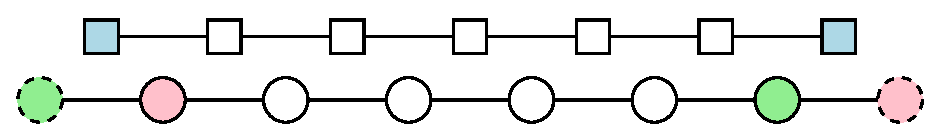
\includegraphics[width=0.9\textwidth]{\dir/figs/grid_ew.eps}
  \caption{A row of the numeric grid when the model is used in torus mode. Circles indicate points in $(i,j)$--grid and squares indicate points in the $(r,s)$--grid. Points with the same color are logically the same.}
  \label{num.fig.grid_ew}
\end{figure}

These boundary conditions are enforced by exchanging points for the temperature and vertical velocity calculations. The ice thicknesses are calculated explicitly at the ghostpoints.

\subsubsection{$\sigma$--Coordinate System}\label{num.sec.sigma}
The vertical coordinate, $z$, is scaled by the ice thickness analogous to the $s$--coordinate in numerical weather simulations \citep[e.g.,][]{Holton1992}. A new vertical coordinate, $\sigma$, is introduced so that the ice surface is at $\sigma=0$ and the ice base at $\sigma=1$ (see Fig. \ref{kin.fig.scale}), i.e.
\begin{equation}
  \label{kin.eq.vertical_scale}
  \sigma=\frac{s-z}{H}.
\end{equation}

\begin{figure}[htbp]
  \begin{center}
    
\includegraphics{\dir/figs/scale.eps}
    \caption[Vertical scaling of the ice sheet model.]{Vertical scaling of the ice sheet model. The vertical axis is scaled to unity. The horizontal coordinates are not changed.}
    \label{kin.fig.scale}
  \end{center}
\end{figure}


The derivatives of a function $f$ in $(x,y,z,t)$ become in the new $(\tilde{x},\tilde{y},\sigma,\tilde{t})$ system:
\begin{subequations}
  \begin{align}
    \frac{\pd f}{\pd x} &= \frac{\pd f}{\pd\tilde{x}}+\frac1H\Delta_{\tilde{x}}\frac{\pd f}{\pd \sigma},\\
    \frac{\pd f}{\pd y} &= \frac{\pd f}{\pd\tilde{y}}+\frac1H\Delta_{\tilde{y}}\frac{\pd f}{\pd \sigma},\\
    \frac{\pd f}{\pd t} &= \frac{\pd f}{\pd\tilde{t}}+\frac1H\Delta_{\tilde{t}}\frac{\pd f}{\pd \sigma},\\
    \frac{\pd f}{\pd z} &= -\frac1H\frac{\pd f}{\pd\sigma},
  \end{align}
\end{subequations}
where  the geometric factors, $\Delta_{\tilde{x}}$, $\Delta_{\tilde{y}}$ and $\Delta_{\tilde{t}}$, are defined by
\begin{subequations}
  \begin{align}
  \Delta_{\tilde{x}}&=\left(\frac{\pd s}{\pd\tilde{x}}-\sigma\frac{\pd H}{\pd\tilde{x}}\right),\\
  \Delta_{\tilde{y}}&=\left(\frac{\pd s}{\pd\tilde{y}}-\sigma\frac{\pd H}{\pd\tilde{y}}\right),\\
  \Delta_{\tilde{t}}&=\left(\frac{\pd s}{\pd\tilde{t}}-\sigma\frac{\pd H}{\pd\tilde{t}}\right).
  \end{align}
\end{subequations}
The integral of $z$ becomes in the $\sigma$--coordinate system:
\begin{equation}
  \int_b^zfdz=-H\int_1^\sigma fd\sigma.
\end{equation}

The vertical coordinate can be discretized using an irregular grid spacing to reflect the fact that ice flow is more variable at the bottom of the ice column. In the vertical the index $k$ is used. 


\subsection{Ice Sheet Equations in $\sigma$--Coordinates}
The horizontal velocity, Equation \eqref{kin.eq.horiz_velo}, becomes in the $\sigma$--coordinate system
\begin{equation}
  \label{kin.eq.vert_velo_sigma}
  \vec u(\sigma) = -2(\rho g)^nH^{n+1}|\vec\nabla s|^{n-1}\vec\nabla s\int_1^\sigma A\sigma^nd\sigma+\vec u(1)
\end{equation}
and the vertically averaged velocity
\begin{equation}
  \label{kin.eq.avg_velo_scaled}
  \overline{\vec u} H=H\int_0^1\vec ud\sigma+\vec u(1)H
\end{equation}
The vertical velocity, Equation \eqref{kin.eq.vert_velo}, becomes
\begin{equation}
  \label{kin.eq.vert_velo_scaled}
  w(\sigma)=-\int_1^\sigma\left(\frac{\pd\vec u}{\pd\sigma}\cdot(\vec\nabla s-\sigma\vec\nabla H)+H\vec\nabla\cdot\vec u\right)d\sigma+w(1)
\end{equation}
and lower boundary condition
\begin{equation}
  w(1)=\frac{\pd h}{\pd t}+\vec u(1)\cdot\vec\nabla h+S.
\end{equation}

\subsection{Calculating the Horizontal Velocity and the Diffusivity}
Horizontal velocity and diffusivity calculations are split up into two parts:
\begin{subequations}
  \label{kin.eq.horiz_diffusivity}
  \begin{align}
    \vec u(\sigma)&=c\vec\nabla s+\vec u(1)\\
    D &=H\int_0^1cd\sigma\\
    \vec q&=D\vec\nabla s+H\vec u(1)\\
    \intertext{with}
    c(\sigma)&=-2(\rho g)^nH^{n+1}|\vec\nabla s|^{n-1}\int_1^\sigma A\sigma^nd\sigma
  \end{align}
\end{subequations}

Quantities $\vec u$ and $D$ are found on the velocity grid. Integrating from the ice base ($k=N-1$), the discretised quantities become
\begin{subequations}
  \begin{equation}
    \tilde{c}_{r,s,N}=0
  \end{equation}
  \begin{multline}
    \tilde{c}_{r,s,k}=-2(\rho g)^nH_{r,s}^{n+1}\left(({\tilde{s}^x_{r,s}})^2+({\tilde{s}^y_{r,s}})^2\right)^{\frac{n-1}{2}}\\
    \sum_{\kappa=N-1}^k\frac{A_{r,s,\kappa}+A_{r,s,\kappa+1}}2 \left(\frac{\sigma_{\kappa+1}+\sigma_\kappa}2\right)^n(\sigma_{\kappa+1}-\sigma_\kappa)
  \end{multline}
  \begin{equation}
    \tilde{D}_{r,s}=H_{r,s}\sum_{k=0}^{N-1}\frac{\tilde{c}_{r,s,k}+\tilde{c}_{r,s,k+1}}2(\sigma_{k+1}-\sigma_k)
  \end{equation}
\end{subequations}
Expressions for $\vec{u}_{i,j,k}$ and $\vec{q}_{i,j}$ are straight forward.

\subsection{Solving the Ice Thickness Evolution Equation}
Equation \eqref{kin.eq.ice_thickness} can be rewritten as a diffusion equation, with non--linear diffusion coefficient $D$:
\begin{equation}
  \label{kin.eq.ice_evo}
  \frac{\pd H}{\pd t}=-\vec\nabla\cdot D\vec\nabla s+B=-\vec\nabla\cdot\vec q+B
\end{equation}
This non--linear partial differential equation can be linearised by using the diffusion coefficient from the previous time step. The diffusion coefficient is calculated on the $(r,s)$--grid, i.e. staggered in both $x$ and $y$ direction. Figure \ref{kin.fig.staggered_grid} illustrates the staggered grid. Using finite differences, the fluxes in $x$ direction, $q^x$ become
\begin{subequations}
\begin{align}
  q^x_{i+\frac12,j}&=-\frac12(\tilde{D}_{r,s}+\tilde{D}_{r,s-1})\frac{s_{i+1,j}-s_{i,j}}{\Delta x}\\
  q^x_{i-\frac12,j}&=-\frac12(\tilde{D}_{r-1,s}+\tilde{D}_{r-1,s-1})\frac{s_{i,j}-s_{i-1,j}}{\Delta x}\\
  \intertext{and the fluxes in $y$ direction}
  q^y_{i,j+\frac12}&=-\frac12(\tilde{D}_{r,s}+\tilde{D}_{r-1,s})\frac{s_{i,j+1}-s_{i,j}}{\Delta y}\\
  q^y_{i,j-\frac12}&=-\frac12(\tilde{D}_{r,s-1}+\tilde{D}_{r-1,s-1})\frac{s_{i,j}-s_{i,j-1}}{\Delta y}.
\end{align}  
\end{subequations}

\begin{figure}[htbp]
  \centering
  
\includegraphics{\dir/figs/staggered_grid.eps}
  \caption{Illustration of the staggered grid used to calculate ice thicknesses, diffusivities and mass fluxes.}
  \label{kin.fig.staggered_grid}
\end{figure}

\subsubsection{ADI Scheme}
The alternating--direction implicit method (ADI) uses the concept of operator splitting where Equation \eqref{kin.eq.ice_evo} is first solved in the $x$--direction and then in the $y$--direction, \citep{Press1992}. The time step $\Delta t$ is devided into two time steps $\Delta t/2$. The descretised version of Equation \eqref{kin.eq.ice_evo} becomes \citep{Huybrechts1986}:
\begin{subequations}
\begin{align}
  \label{kin.eq.adi_1}
  2\frac{H_{i,j}^{t+\frac12}-H_{i,j}^{t}}{\Delta t} &= -\frac{q_{i+\frac12,j}^{x,t+\frac12}-q_{i-\frac12,j}^{x,t+\frac12}}{\Delta x} - \frac{q_{i,j+\frac12}^{y,t}-q_{i,j-\frac12}^{y,t}}{\Delta y} + B_{i,j} \\
  \label{kin.eq.adi_2}
  2\frac{H_{i,j}^{t+1}-H_{i,j}^{t+\frac12}}{\Delta t} &= -\frac{q_{i+\frac12,j}^{x,t+\frac12}-q_{i-\frac12,j}^{x,t+\frac12}}{\Delta x} - \frac{q_{i,j+\frac12}^{y,t+1}-q_{i,j-\frac12}^{y,t+1}}{\Delta y} + B_{i,j}
\end{align}
\end{subequations}
Gathering all $t+\frac12$ terms on the left side, Equation \eqref{kin.eq.adi_1} can be expressed as a tri--diagonal set of equations for each row $j$:
\begin{equation}
  -\alpha_{i,j}H_{i-1,j}^{t+\frac12} + (1-\beta_{i,j})H_{i,j}^{t+\frac12} - \gamma_{i,j}H_{i+1,j}^{t+\frac12} = \delta_{i,j}
\end{equation}
with
\begin{subequations}
  \begin{align}
  \alpha_{i,j} &=\frac{\tilde{D}_{r-1,s}+\tilde{D}_{r-1,s-1}}{4\Delta x^2}\Delta t\\
  \beta_{i,j}  &=-\frac{\tilde{D}_{r,s}+2\tilde{D}_{r-1,s}+\tilde{D}_{r-1,s-1}}{4\Delta x^2}\Delta t = -(\alpha_{i,j}+\gamma_{i,j})\\
  \gamma_{i,j} &=\frac{\tilde{D}_{r,s}+\tilde{D}_{r,s-1}}{4\Delta x^2}\Delta t    
  \end{align}
and the RHS,
\begin{equation}
  \delta_{i,j} = H_{i,j}^t-\frac{\Delta t}{2\Delta y}\left(q_{i,j+\frac12}^{y,t}-q_{i,j-\frac12}^{y,t}\right) + \frac{\Delta t}2B_{i,j} + \alpha_{i,j}h_{i-1,j} -\beta_{i,j}h_{i,j} + \gamma_{i,j}h_{i+1,j}.
\end{equation}
\end{subequations}

A similar tri--diagonal system is found for each column, $i$ of Equation \eqref{kin.eq.adi_2}.

\subsubsection{Linearised Semi--Implicit Scheme}
Using the Crank--Nicolson scheme, the semi--implicit temporal discretisation of \eqref{kin.eq.ice_evo} is then:
\begin{multline}
\label{kin.eq.ice_evo_disc1}
  \frac{H^{t+1}_{i,j}-H^t_{i,j}}{\Delta t}=\frac{q^{x,t+1}_{i+\frac12,j}-q^{x,t+1}_{i-\frac12,j}}{2\Delta x}+\frac{q^{y,t+1}_{i,j+\frac12}-q^{y,t+1}_{i,j-\frac12}}{2\Delta y} \\
  +\frac{q^{x,t}_{i+\frac12,j}-q^{x,t}_{i-\frac12,j}}{2\Delta x}+\frac{q^{y,t}_{i,j+\frac12}-q^{y,t}_{i,j-\frac12}}{2\Delta y}+ B_{i,j}
\end{multline}
The superscripts $^t$ and $^{t+1}$ indicate at what time the ice thickness $H$ is evaluated. Collecting all $H^{t+1}$ terms of \eqref{kin.eq.ice_evo_disc1} on the LHS and moving all other terms to the RHS we can rewrite \eqref{kin.eq.ice_evo_disc1} as
\begin{equation}
  \label{kin.eq.evo_matrix}
  -\alpha_{i,j}H^{t+1}_{i-1,j} - \beta_{i,j}H^{t+1}_{i+1,j} - \gamma_{i,j}H^{t+1}_{i,j-1} - \delta_{i,j}H^{t+1}_{i,j+1}+ (1-\epsilon_{i,j})H^{t+1}_{i,j} = \zeta_{i,j}
\end{equation}
with the RHS,
\begin{multline}
  \zeta_{i,j} = \alpha_{i,j}H^{t}_{i-1,j} + \beta_{i,j}H^{t}_{i+1,j} + \gamma_{i,j}H^{t}_{i,j-1} + \delta_{i,j}H^{t}_{i,j+1} + (1+\epsilon_{i,j})H^{t}_{i,j} \\
  + 2(\alpha_{i,j}h_{i-1,j} + \beta_{i,j}h_{i+1,j} + \gamma_{i,j}h_{i,j-1} + \delta_{i,j}h_{i,j+1}+ \epsilon_{i,j}h_{i,j}) + B_{i,j}\Delta t
\end{multline}
with the elements of the sparse matrix
\begin{subequations}
  \begin{align}
    \alpha_{i,j} &=\frac{\tilde{D}_{r-1,s}+\tilde{D}_{r-1,s-1}}{4\Delta x^2}\Delta t\\
    \beta_{i,j} &=\frac{\tilde{D}_{r,s}+\tilde{D}_{r,s-1}}{4\Delta x^2}\Delta t\\
    \gamma_{i,j} &=\frac{\tilde{D}_{r,s-1}+\tilde{D}_{r-1,s-1}}{4\Delta y^2}\Delta t\\
    \delta_{i,j} &=\frac{\tilde{D}_{r,s}+\tilde{D}_{r-1,s}}{4\Delta y^2}\Delta t\\
    \epsilon_{i,j} &=-(\alpha_{i,j}+\beta_{i,j}+\gamma_{i,j}+\delta_{i,j})
  \end{align}
\end{subequations}

This matrix equation is solved using an iterative matrix solver for non-symmetric sparse matrices. The solver used here is the bi--conjugate gradient method with incomplete LU decomposition preconditioning provided by the SLAP package.

\subsubsection{Non--Linear Scheme}
The non--linearity of Equation \eqref{kin.eq.ice_evo} arises from the dependance of $D$ on $s$. A non--linear scheme for \eqref{kin.eq.ice_evo} can be formulated using Picard iteration, which consists of two iterations: an outer, non--linear and an inner, linear equation. The scheme is started off with the diffusivity from the previous time step, i.e.
\begin{subequations}
  \begin{equation}
    D^{(0),t+1}=D^{t}
  \end{equation}
and Equation \eqref{kin.eq.evo_matrix} becomes
\begin{multline}
  \label{kin.eq.evo_matrix_nonlin}
  -\alpha^{(\xi),t+1}_{i,j}H^{t+1}_{i-1,j} - \beta^{(\xi),t+1}_{i,j}H^{(\xi+1),t+1}_{i+1,j} - \gamma^{(\xi),t+1}_{i,j}H^{(\xi+1),t+1}_{i,j-1} \\
  - \delta^{(\xi),t+1}_{i,j}H^{(\xi+1),t+1}_{i,j+1}+ (1-\epsilon^{(\xi),t+1}_{i,j})H^{(\xi+1),t+1}_{i,j} = \zeta^{(0),t}_{i,j}
\end{multline}
\end{subequations}
Equation \eqref{kin.eq.evo_matrix_nonlin} is iterated over $\xi$ until the maximum ice thickness residual is smaller than some threshold:
\begin{equation}
  \max\left(\left|H^{(\xi+1),t+1}-H^{(\xi),t+1}\right|\right)<H_{\text{res}}
\end{equation}

\begin{figure}[htbp]
  \centering
  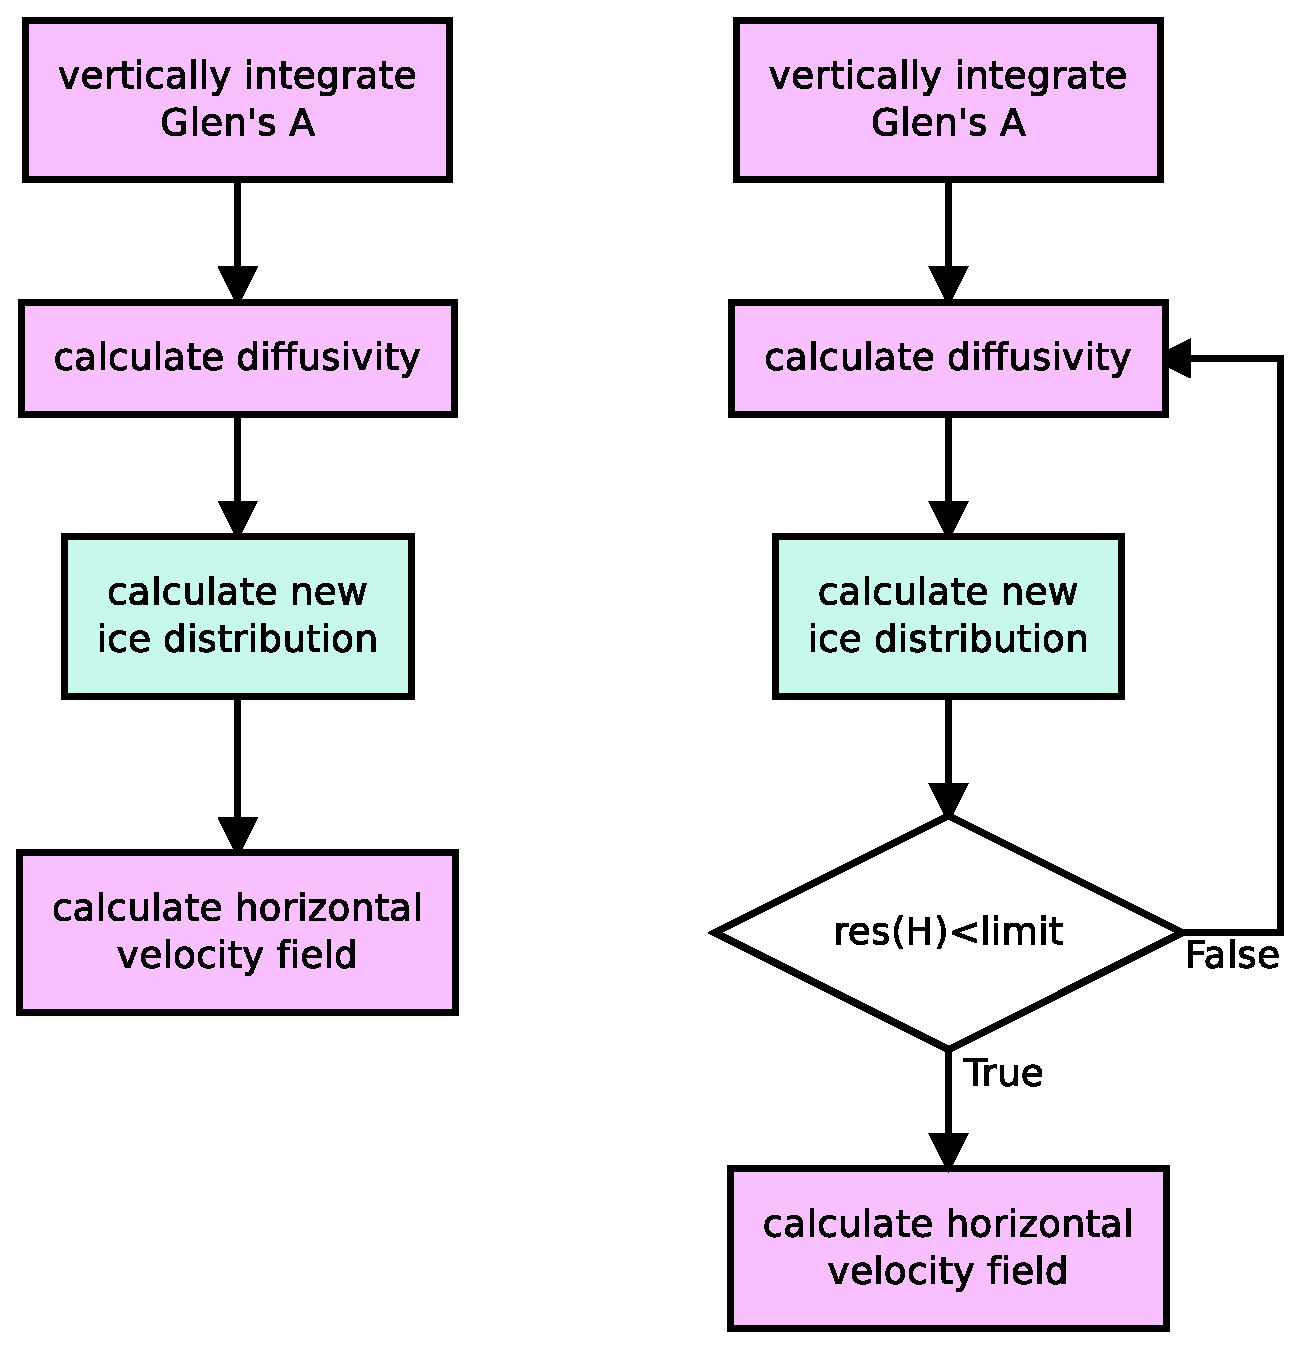
\includegraphics[width=0.5\textwidth]{\dir/figs/thick_evo.eps}
  \caption{Flow diagram showing how the linearised solver (on the left) and the non--linear solver work. The inner, linear iteration is contained within the box labeled ``calculate new ice distribution''.}
  \label{kin.fig.solvers}
\end{figure}

\subsection{Calculating Vertical Velocities}

\subsubsection{Grid Velocity}
The vertical grid moves as a result of using a $\sigma$--coordinate system. The grid velocity is
\begin{equation}
  \label{kin.eq.grid_velo}
  w^{\text{grid}}(\sigma)=\frac{\pd s}{\pd t}+\vec u\cdot\vec\nabla s-\sigma\left(\frac{\pd H}{\pd t}+\vec u\cdot\vec\nabla H\right).
\end{equation}
The numerical implementation of \eqref{kin.eq.grid_velo} is straightforward.

\subsubsection{Vertical Velocity}
The discretized version of the vertical velocity equation \eqref{kin.eq.vert_velo_scaled} is slightly more compilicated because the horizontal velocities are calculated on the $(r,s)$ grid. The vertical velocity at the ice base is $w_{i,j,N}=w^{\text{grid}}_{i,j,N}-M_b{i,j}$, where $M_b{i,j}$ is the basal melt rate. Integrating from the bottom, the vertical velocity is then
\begin{equation}
  \label{kin.eq.wvel_unc}
  \begin{split}
  w_{i,j,k}=-\sum_{\tilde{k}=N-1}^1\left\{\mathcal{H}_{i,j}\left(\frac{u^x_{i,j,k}+u^x_{i,j,k+1}}{2}+\frac{v^y_{i,j,k}+v^y_{i,j,k+1}}{2}\right)(\sigma_{k+1}-\sigma_k)\right. \\
     +(\tilde{u}_{i,j,k+1}-\tilde{u}_{i,j,k})  \left(\tilde{s}^x_{i,j}-\frac12(\sigma_{k+1}+\sigma_k)\tilde{H}^x_{i,j}\right)  \\
     \left.+(\tilde{v}_{i,j,k+1}-\tilde{v}_{i,j,k})  \left(\tilde{s}^y_{i,j}-\frac12(\sigma_{k+1}+\sigma_k)\tilde{H}^y_{i,j}\right)\right\} + w_{i,j,N},
  \end{split}
\end{equation}
with the weighted ice thickness
\begin{equation*}
  \begin{split}
  \mathcal{H}_{i,j}=\frac{4H_{i,j}+2(H_{i-1,j}+H_{i+1,j}+H_{i,j-1}+H_{i,j+1})}{16}\\
  +\frac{H_{i-1,j-1}+H_{i+1,j-1}+H_{i+1,j+1}+H_{i-1,j+1}}{16}.    
  \end{split}
\end{equation*}

This scheme produces vertical velocities at the ice divide which are too small. The vertical velocities on the ice surface are given by the upper kinematic boundary condition \eqref{kin.eq.upper_bc}. Equation \eqref{kin.eq.wvel_unc} can be corrected with
\begin{equation}
  \label{kin.eq.wvel_cor}
   w^\ast_{i,j,k}=w_{i,j,k}-(1-\sigma_k)(w_{i,j,k}-{w_s}_{i,j}),
\end{equation}
where ${w_s}_{i,j}$ is the vertical velocity at the ice surface given by \eqref{kin.eq.upper_bc}. Figure \ref{kin.fig.w_profile} shows the different vertical velocities at the ice surface.
\begin{figure}[htbp]
  \centering
  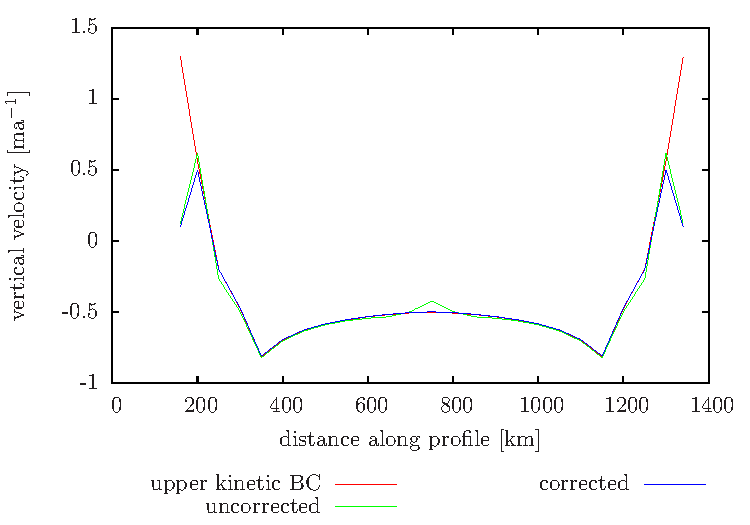
\includegraphics{\dir/gnu/w_profile.eps}
  \caption{Vertical ice surface velocities of the EISMINT-1 moving margin experiment.}
  \label{kin.fig.w_profile}
\end{figure}
The difference between the vertical velocities calculated by the model and the vertical velocities given by \eqref{kin.eq.upper_bc} at the ice margin are due to the fact that temperatures and velocities are only calculated when the ice is thicker than a certain threshold value which is not met at the ice margin.

Figure \ref{kin.fig.wt_sigma} shows vertical profiles of the vertical velocity at the ice divide and a point halfway between the divide and the domain margin. A corresponding temperature profile is also shown since the vertical velocity determines the vertical temperature advection (see Section \ref{temp.sec.vert_ad}).
\begin{figure}[htbp]
  \centering
  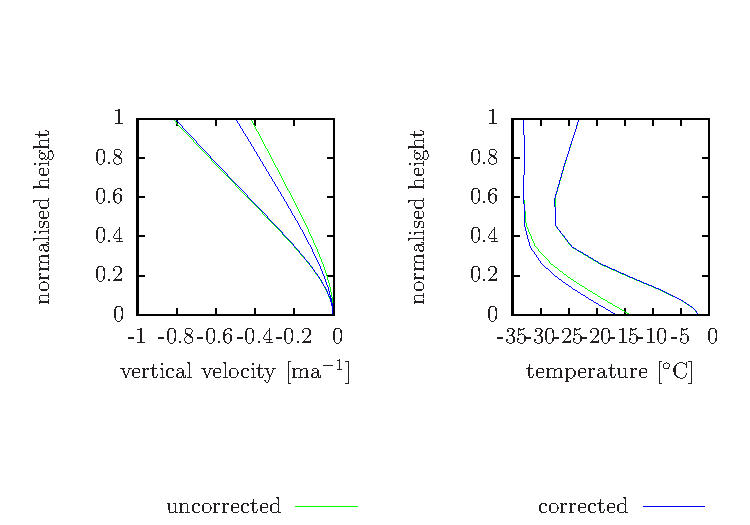
\includegraphics{\dir/gnu/wt_sigma.eps}
  \caption{Vertical velocity and temperature distribution for columns at the ice divide and a point halfway between the divide and the domain margin.}
  \label{kin.fig.wt_sigma}
\end{figure}


\section{Temperature Solver}
The flow law, Equation \eqref{kin.eq.flowlaw}, depends on the temperature of ice. It is, therefore, necessary to determine how the distribution of ice temperatures changes with a changing ice sheet configuration. The thermal evolution of the ice sheet is described by
\begin{equation}
  \label{temp.eq.temp_z}
  \frac{\pd T}{\pd t}=\frac{k}{\rho c}\nabla^2T-\vec{u}\cdot\vec\nabla T+\frac\Phi{\rho c}-w\frac{\pd T}{\pd z},
\end{equation}
where $T$ is the absolute temperature, $k$ is the thermal conductivity of ice, $c$ is the specific heat capacity and $\Phi$ is the heat generated due to internal friction. In the $\sigma$--coordinate system, Equation \eqref{temp.eq.temp_z}, becomes
\begin{equation}
  \label{temp.eq.temp}
  \frac{\pd T}{\pd t} = \frac{k}{\rho cH^2}\frac{\pd^2T}{\pd\sigma^2} - \vec{u}\cdot\vec\nabla T + \frac{\sigma g}c\frac{\pd \vec{u}}{\pd\sigma}\cdot\vec\nabla s + \frac1H\frac{\pd T}{\pd\sigma}\left(w-w_{\text{grid}}\right)
\end{equation}
The terms represents (1) vertical diffusion, (2) horizontal advection, (3) internal heat generation due to friction and (4) vertical advection and a correction due to the sigma coordinate system. Let's rewrite \eqref{temp.eq.temp} to introduce some names:
\begin{equation}
  \label{temp.eq.temp2}
  \frac{\pd T}{\pd t} = a\frac{\pd^2T}{\pd\sigma^2} +b(\sigma) + \Phi(\sigma) + c(\sigma)\frac{\pd T}{\pd\sigma},
\end{equation}
where
\begin{subequations}
  \begin{align}
    a&=\frac{k}{\rho cH^2} \\
    \label{temp.eq.hadv}
    b(\sigma)&=-\vec{u}\cdot\vec\nabla T\\
    \Phi(\sigma)&=\frac{\sigma g}c\frac{\pd \vec{u}}{\pd\sigma}\cdot\vec\nabla s \\
    c(\sigma)&=\frac1H\left(w-w_{\text{grid}}\right)
  \end{align}
\end{subequations}

\subsection{Vertical Diffusion}
Discretisation of $\pd^2T/\pd\sigma^2$ is slightly complicated because the vertical grid is irregular. Using Taylor series the central difference formulas are
\begin{subequations}
  \begin{align}
    \label{temp.eq.d1}
    \left.\frac{\pd T}{\pd\sigma}\right|_{\sigma_{k-1/2}}&=\frac{T_k-T_{k-1}}{\sigma_k-\sigma_{k-1}}\\
    \intertext{and}
    \label{temp.eq.d2}
    \left.\frac{\pd T}{\pd\sigma}\right|_{\sigma_{k+1/2}}&=\frac{T_{k+1}-T_k}{\sigma_{k+1}-\sigma_k}\\
    \intertext{The second partial derivative is then, also using central differences:}
    \label{temp.eq.d3}
    \left.\frac{\pd^2 T}{\pd\sigma^2}\right|_{\sigma_k} &= \frac{\left.{\pd T}/{\pd\sigma}\right|_{\sigma_{k+1/2}} - \left.{\pd T}/{\pd\sigma}\right|_{\sigma_{k-1/2}}}{1/2\left(\sigma_{k+1}-\sigma_{k-1}\right)}\\
    \intertext{Inserting \eqref{temp.eq.d1} and \eqref{temp.eq.d2} into \eqref{temp.eq.d3}, we get:}
    \label{temp.eq.d4}
    &=\frac{2(T_{k+1}-T_k)}{(\sigma_{k+1}-\sigma_k)(\sigma_{k+1}-\sigma_{k-1})}-\frac{2(T_k-T_{k-1})}{(\sigma_k-\sigma_{k-1})(\sigma_{k+1}-\sigma_{k-1})}
  \end{align}
\end{subequations}
Finally, the terms of equation \eqref{temp.eq.d4} are rearranged:
\begin{multline}
  \label{temp.eq.dsigma2}
  \left.\frac{\pd^2 T}{\pd\sigma^2}\right|_{\sigma_k} = \frac{2T_{k-1}}{(\sigma_k-\sigma_{k-1})(\sigma_{k+1}-\sigma_{k-1})} - \frac{2T_k}{(\sigma_{k+1}-\sigma_k)(\sigma_k-\sigma_{k-1})}\\
  + \frac{2T_{k+1}}{(\sigma_{k+1}-\sigma_k)(\sigma_{k+1}-\sigma_{k-1})}
\end{multline}

\subsection{Horizontal Advection}
The horizontal advection term, $- \vec{u}\cdot\vec\nabla T$ is solved using an upwinding scheme. Let's start with the 1--dimensional case. The method discussed can be straightforwadly extented to 2D. As always, the temperature function is expressed as a Taylor series.
\begin{subequations}
  \begin{align}
    \label{temp.eq.taylor1}
    T(x+\Delta x) &=T(x)+\Delta xT'(x)+\frac{\Delta x^2}2T''(x)+\ldots\\
    \intertext{If we subsitute $\Delta x$ with $2\Delta x$, Equation \eqref{temp.eq.taylor1}}
    \label{temp.eq.taylor2}
    T(x+2\Delta x) &=T(x)+2\Delta xT'(x)+2\Delta x^2T''(x)+\ldots
  \end{align}
\end{subequations}
From \eqref{temp.eq.taylor1} and \eqref{temp.eq.taylor2} we can construct a difference formula where the $\mathcal{O}(\Delta x^2)$ error is cancelled, by multiplying \eqref{temp.eq.taylor1} with 4 and substracting the result from \eqref{temp.eq.taylor2}:
\begin{subequations}
  \begin{align}
    \label{temp.eq.forward_h3}
    T_+'(x)&=\frac{4T(x+\Delta x)-T(x+2\Delta x)-3T(x)}{2\Delta x}\\
    \intertext{and similarly for the backward difference:}
    T_-'(x)&=-\frac{4T(x-\Delta x)-T(x-2\Delta x)-3T(x)}{2\Delta x}
    \end{align}
\end{subequations}
So the horizontal advection term in one dimensions becomes:
\begin{equation}
  b_x = -u_x\frac{\pd T}{\pd x}=\frac{-u_x}{2\Delta x}
  \begin{cases}
    -(4T_{i-1}-T_{i-2}-3T_i) & \text{when $u_x>0$} \\
    4T_{i+1}-T_{i+2}-3T_i & \text{when $u_x<0$} \\
  \end{cases}
\end{equation}
A similar expression is found for $b_y$ by simply substituting $y$ for $x$. Finally, the combined horizontal advection term, is simply
\begin{equation}
  b=-\vec{u}\cdot\vec\nabla T=-\left(u_x\frac{\pd T}{\pd x}+u_y\frac{\pd T}{\pd y}\right)=b_x+b_y=b_1+b_2T_i
\end{equation}

\subsection{Heat Generation}
Taking the derivative of \eqref{kin.eq.vert_velo_sigma} with respect to $\sigma$, we get
\begin{equation}
  \frac{\pd u_x}{\pd\sigma} = -2(\rho g)^nH^{n+1}|\vec\nabla s|^{n-1}\frac{\pd s}{\pd x}A(T^\ast)\sigma^n
\end{equation}
Thus,
\begin{equation}
\begin{split}
  \Phi(\sigma) &= \frac{\sigma g}c\frac{\pd \vec{u}}{\pd\sigma}\cdot\vec\nabla s  = \frac{\sigma g}c\left(\frac{\pd u_x}{\pd \sigma}\frac{\pd s}{\pd x} + \frac{\pd u_y}{\pd \sigma}\frac{\pd s}{\pd y}\right)\\
       &= -2(\rho g)^nH^{n+1}|\vec\nabla s|^{n-1}\frac{\sigma g}cA(T^\ast)\sigma^n \left(\left(\frac{\pd s}{\pd x}\right)^2+\left(\frac{\pd s}{\pd y}\right)^2\right) \\
       &= -\frac2{c\rho}(g\sigma\rho)^{n+1}\left(H|\vec\nabla s|\right)^{n+1}A(T^\ast)
\end{split}  
\end{equation}

The constant factor $\frac2{c\rho}(g\sigma\rho)^{n+1}$ is calculated during initialisation in the subroutine \texttt{init\_temp}. This factor is assigned to array \texttt{c1(1:upn)}. \texttt{c1} also includes various scaling factors and the factor $1/16$ to normalise $\mathcal{A}$.

The next factor, $\left(H|\vec\nabla s|\right)^{n+1}$ is calculated in the subroutine \texttt{finddisp}:
\begin{equation}
  {c_2}_{i,j} = \left(\tilde{H}_{i,j}\sqrt{\tilde{S_x}_{i,j}^2+\tilde{S_y}_{i,j}^2}\right)^{n+1},
\end{equation}


The final factor is found by averaging over the neighbouring nodes:
\begin{equation}
  \mathcal{A}_{i,j}=4A_{i,j}+2(A_{i-1,j}+A_{i+1,j}+A_{i,j-1}+A_{i,j+1})+(A_{i-1,j-1}+A_{i+1,j-1}+A_{i+1,j+1}+A_{i-1,j+1})
\end{equation}

\subsection{Vertical Advection}\label{temp.sec.vert_ad}
The vertical advection term, $\pd T/\pd\sigma$ is solved using the central difference formula for unevenly spaced nodes:
\begin{equation}
  \frac{\pd T}{\pd\sigma}=\frac{T_{k+1}-T_{k-1}}{\sigma_{k+1}-\sigma_{k-1}}
\end{equation}

\subsection{Boundary Conditions}
At the upper boundary, ice temperatures are set to the surface temperature, $T_{\text{surf}}$. The ice at the base is heated by the geothermal heat flux and sliding friction:
\begin{equation}
  \left.\frac{\pd T}{\pd\sigma}\right|_{\sigma=1}=-\frac{GH}k-\frac{H\vec{\tau}_b\cdot\vec{u}(1)}k,
\end{equation}
where $\vec{\tau}_b=-\rho gH\vec\nabla s$ is the basal shear stress and $\vec{u}(1)$ is the basal ice velocity. Ice temperatures are held constant if they reach the pressure melting point of ice, i.e.
\begin{equation}
  T^\ast=T_{\text{pmp}} \quad\text{if $T\ge T_{\text{pmp}}$}.
\end{equation}
Excess heat is then used to formulate a melt rate, $S$:
\begin{equation}
  \label{temp.eq.meltrate}
  S=\frac{k}{\rho L}\left(\frac{\pd T^\ast}{\pd z}-\frac{\pd T}{\pd z}\right),
\end{equation}
where $L$ is the specific latent heat of fusion. Finally, basal temperatures are held constant, if the ice is floating:
\begin{equation}
  \frac{\pd T(1)}{\pd t}  = 0.
\end{equation}


\subsection{Putting it all together}
Equation \eqref{temp.eq.temp} is solved for each ice column. The horizontal dependency of the horizontal advection term, \eqref{temp.eq.hadv}, is resolved by iterating the vertical solution. Putting the individual terms together using a fully explicit finite differences scheme, Equation \eqref{temp.eq.temp2} becomes
\begin{subequations}
  \begin{multline}
    \label{temp.eq.temp3a}
    \frac{T_{k,t+1}-T_{k,t}}{\Delta t} = \left(\frac{2aT_{k-1,t}}{(\sigma_k-\sigma_{k-1})(\sigma_{k+1}-\sigma_{k-1})} - \frac{2aT_{k,t}}{(\sigma_{k+1}-\sigma_k)(\sigma_k-\sigma_{k-1,t})}\right. \\
    \left.+ \frac{2aT_{k+1,t}}{(\sigma_{k+1}-\sigma_k)(\sigma_{k+1}-\sigma_{k-1})}\right)+{b_1}_{k,t}+{b_2}_kT_{k,t}+\Phi_k+c_k\frac{T_{k+1,t}-T_{k-1,t}}{\sigma_{k+1}-\sigma_{k-1}}
\end{multline}
and similarly the fully implicit scheme
  \begin{multline}
    \label{temp.eq.temp3b}
    \frac{T_{k,t+1}-T_{k,t}}{\Delta t} = \left(\frac{2aT_{k-1,t+1}}{(\sigma_k-\sigma_{k-1})(\sigma_{k+1}-\sigma_{k-1})} - \frac{2aT_{k,t+1}}{(\sigma_{k+1}-\sigma_k)(\sigma_k-\sigma_{k-1,t+1})}\right. \\
    \left.+ \frac{2aT_{k+1,t+1}}{(\sigma_{k+1}-\sigma_k)(\sigma_{k+1}-\sigma_{k-1})}\right)+{b_1}_{k,t+1}+{b_2}_kT_{k,t+1}+\Phi_k+c_k\frac{T_{k+1,t+1}-T_{k-1,t+1}}{\sigma_{k+1}-\sigma_{k-1}}
\end{multline}
\end{subequations}
Taking the average of Equations \eqref{temp.eq.temp3a} and \eqref{temp.eq.temp3b} gives the \emph{Crank--Nicholson scheme}. The resulting equation is then rearranged and terms of $T_{k-1,t+1}$, $T_{k,t+1}$ and $T_{k+1,t+1}$ are combined to give the tri--diagonal system
\begin{equation}
  \alpha_kT_{k-1,t+1}+\beta_kT_{k,t+1}+\gamma_kT_{k+1,t+1}=\delta_k
\end{equation}
where, for $k=2,N-1$
\begin{subequations}
  \begin{align}
    \alpha_k &= -\frac12\frac{2a\Delta t}{(\sigma_k-\sigma_{k-1})(\sigma_{k+1}-\sigma_{k-1})}+\frac12\frac{c_k\Delta t}{\sigma_{k+1}-\sigma_{k-1}} \\
    \beta_k &= 1+\frac12\frac{2a\Delta t}{(\sigma_{k+1}-\sigma_k)(\sigma_k-\sigma_{k-1})}-\frac12{b_2}_k\Delta t=1-\alpha_k-\gamma_k-\frac12{b_2}_k\Delta t\\
    \gamma_k &= -\frac12\frac{2a\Delta t}{(\sigma_{k+1}-\sigma_k)(\sigma_{k+1}-\sigma_{k-1})}-\frac12\frac{c_k\Delta t}{\sigma_{k+1}-\sigma_{k-1}} \\
    \delta_k &= -\alpha_kT_{k-1,t}+(2-\beta_k)T_{k,t}-\gamma_kT_{k+1,t}+\frac12({b_1}_{k,t}+{b_1}_{k,t+1})\Delta t+\Phi_k\Delta t
  \end{align}

\subsubsection{Boundary Conditions}
At the upper boundary:
\begin{equation}
  \alpha_1=0,\quad\beta_1=1,\quad\gamma_1=0,\quad\delta_1=T_{\text{surf}}
\end{equation}
\end{subequations}


The lower boundary condition is somewhat more complicated. Here we only look at the case when the temperature is below the pressure melting point of ice. BC for floating ice and temperatures at the pressure melting point of ice are trivial. The geothermal heat flux is applied at the lower boundary, i.e. Equation \eqref{temp.eq.d2} becomes
\begin{equation}
  \label{temp.eq.d2-lb}
  \left.\frac{\pd T}{\pd\sigma}\right|_{\sigma_{k+1/2}}=-\frac{GH}k
\end{equation}
Assuming that $\sigma_k-\sigma_{k-1}=\sigma_{k+1}-\sigma_k=\Delta\sigma$ and inserting \eqref{temp.eq.d1} and \eqref{temp.eq.d2-lb} into \eqref{temp.eq.d3}, the second partial derivative becomes
\begin{equation}
  \left.\frac{\pd^2 T}{\pd\sigma^2}\right|_{\sigma_N} = \left(-\frac{GH}k-\frac{T_N-T_{N-1}}{\Delta\sigma}\right)/\Delta\sigma=-\frac{GH}{k\Delta\sigma}-\frac{T_N-T_{N-1}}{\Delta\sigma^2}
\end{equation}
Inserting the new conduction term and replacing the derivative of the vertical advection term with the Neumann boundary condition, Equation \eqref{temp.eq.temp3a} becomes
\begin{subequations}
  \begin{equation}
    \frac{T_{N,t+1}-T_{N,t}}{\Delta t} = -a\left(\frac{GH}{k\Delta\sigma}+\frac{T_{N,t}-T_{N-1,t}}{\Delta\sigma^2}\right)+{b_1}_{N,t}+{b_2}_NT_{N,t}+\Phi_N-c_N\frac{GH}k
  \end{equation}
  and similarly for Equation \eqref{temp.eq.temp3b}
  \begin{multline}
    \frac{T_{N,t+1}-T_{N,t}}{\Delta t} = -a\left(\frac{GH}{k\Delta\sigma}+\frac{T_{N,t+1}-T_{N-1,t+1}}{\Delta\sigma^2}\right)+{b_1}_{N,t+1}+{b_2}_NT_{N,t+1}\\
    +\Phi_N-c_N\frac{GH}k
  \end{multline}
\end{subequations}
The elements of the tri--diagonal system at the lower boundary are then
\begin{subequations}
  \begin{gather}
    \alpha_N =-\frac{a\Delta t}{2(\sigma_N-\sigma_{N-1})^2}\\
    \beta_N = 1-\alpha_N+\frac12{b_2}_N\Delta t\\
    \gamma_N = 0 \\
    \begin{split}
      \delta_N =&-\alpha_NT_{N-1,t}+(2-\beta_N)T_{N,t}-a\frac{GH\Delta t}{k(\sigma_N-\sigma_{N-1})}\\
      &+\frac12({b_1}_{N,t}+{b_1}_{N,t+1})\Delta t+\Phi_N\Delta t-c_N\frac{GH\Delta t}k
    \end{split}
  \end{gather}
\end{subequations}


\section{Basal Boundary Condition}
This section describes the formulation of the basal boundary condition.
An interface for the upper boundary condition (atmospheric BC) is easily defined by the surface temperature and mass balance. Similarly, the basal boundary consists of mechanical and thermal boundary conditions. The complications arise because the thermal and mechanical boundary conditions depend on each other. The interface of the basal boundary can be described with the following fields (see also Fig. \ref{num.fig.basal_bc}):
\begin{enumerate}
\item \textbf{basal traction:} This field specifies a parameter which is used to allow basal sliding.
\item \textbf{basal heat flux:} This is the heat flux entering the ice sheet from below.
\item \textbf{basal water depth:} The presence of basal melt water affects the basal ice temperature.
\end{enumerate}
Also, the ice sheet model calculates a melt/freeze rate based on the temperature gradient and basal water depth. This is handled by Glide.

\begin{figure}[htbp]
  \centering
  
\includegraphics[width=0.9\textwidth]{\dir/figs/basal_bc.eps}
  \caption{Basal boundary condition.}
  \label{num.fig.basal_bc}
\end{figure}

\subsection{Mechanical boundary conditions}
If the ice is not frozen to the bed, basal d\'{e}collement may occur. This can be parameterized by a traction factor, $t_b$. 
Within the ice sheet model, $t_b$ can be used to calculate basal sliding velocities $\vec{u}_b$ in the case of zero--order physics. That is,
\begin{equation}
  \vec{u}_b=t_b\vec{\tau}_b,
\end{equation}
where $\tau_b$ is the basal shear stress. Alternatively, $t_b$ can be used as part of the stress--balance calculations when the model is used with higher order physics. In simple models $t_b$ may be uniform or prescribed as a spatial variable. More complex models may wish to make $t_b$ dependent on other variables, such as basal melt rate. Typically $t_b$ will depend on the presence of basal water.

The second mechanical boundary condition, basal melting/freeze--on $M_b$, is handled within the ice sheet model. The details are described in Section \ref{num.sec.bc_melt}.

\subsection{Thermal boundary conditions}
The thermal boundary condition at the ice base is more complicated than the mechanical BC. The ice is heated from below by the geothermal heat flux. Heat is generated by friction with the bed. Furthermore, the ice temperature is constrained to be less than or equal to the pressure melting point of ice. The thermal boundary condition is a flux condition if there is no water present. If there is water, the basal temperature is set to the pressure melting temperature. (If it were lower, there would be no water, and if it were higher, there would be no ice.)

\subsubsection{Basal melting and freezing}\label{num.sec.bc_melt}
At the ice base, $z=b$, we can define outgoing and incoming heat fluxes, $H_o$ and $H_i$:
\begin{subequations}
  \begin{align}
    H_o&=-k_{\text{ice}}\left.\frac{\pd T}{\pd z}\right|_{z=b^+}\\
    \intertext{and}
    H_i&=-k_{\text{rock}}\left.\frac{\pd T}{\pd z}\right|_{z=b^-}+\vec{u}_b\cdot\vec{\tau}_b+
    \begin{cases}
      {\rho_{\text{ice}}M_b}/{L} & \text{when $M_b<0$} \\
      0 & \text{otherwise}
    \end{cases}
  \end{align}
\end{subequations}
where $k_{\text{ice}}$ and $k_{\text{rock}}$ are the thermal conductivities of ice and rock, $\vec{u}_b\cdot\vec{\tau}_b$ is the heat generated by friction with the bed, and $L$ is the latent heat of fusion. The basal melt/freeze--on rate $M_b$ can then be calculated from the difference between the incoming and outgoing heat fluxes:
\begin{equation}
  \label{bc.eq.meltrate}
  M_b=\frac{H_i-H_o}{\rho_{\text{ice}}L}
\end{equation}
There is freeze--on if $M_b < 0$, and basal melting if $B_b > 0$.

\subsubsection{Geothermal Heat Flux}
The heat flux accross the basal boundary depends on past temperature variations since temperature perturbations penetrate the bed rock if the ice is frozen to the ground \citep{Ritz1987}. 
The heat equation for the bed rock layer is given by the diffusion equation
\begin{equation}
  \label{num.eq.diffu_rock}
  \frac{\pd T}{\pd t} = \frac{k_{\text{rock}}}{\rho_{\text{rock}}c_{\text{rock}}}\nabla^2T=\frac{k_{\text{rock}}}{\rho_{\text{rock}}c_{\text{rock}}} 
  \left(\frac{\pd^2 T}{\pd x^2}+\frac{\pd^2 T}{\pd y^2}+\frac{\pd^2 T}{\pd z^2}\right),
\end{equation}
where $k_{\text{rock}}$ is the thermal conductivity, $\rho_{\text{rock}}$ the density and $c_{\text{rock}}$ the specific heat capacity of the bed rock layer. 

Initial conditions for the temperature field $T$ are found by applying the geothermal heat flux, $G$ to an arbitrary surface temperature $T_0$:
\begin{equation}
  T(x,y,z)=T_0+\frac{G}{k_{\text{rock}}}z.
\end{equation}
This ensures that initially the geothermal heat flux experienced by the ice sheet is equal to the regional heat flux. The basal boundary condition of the bedrock layer is kept constant, i.e.
\begin{equation}
  T(x,y,H_{\text{rock}})=T_0+\frac{G}{k_{\text{rock}}}H_{\text{rock}}.
\end{equation}
Lateral boundary conditions are given by
\begin{equation}
  \left.\frac{\pd T}{\pd x}\right|_{x=0} = \left.\frac{\pd T}{\pd x}\right|_{x=L_x} = \left.\frac{\pd T}{\pd y}\right|_{y=0} = \left.\frac{\pd T}{\pd y}\right|_{y=L_y} = 0.
\end{equation}
At the upper boundary, the heat flux of the rock layer has to be matched with the heat flux in the basal ice layer when the ice is frozen to the bed, i.e.
\begin{equation}
  \label{num.eq.gthf_bc}
  k_{\text{rock}}\left.\frac{\pd T}{\pd z}\right|_{z=-0}=k_{\text{ice}}\left.\frac{\pd T}{\pd z}\right|_{z=+0}.
\end{equation}
Otherwise the temperature of the top bedrock layer is set to the surface temperature (if the cell has been occupied by ice, but there is no ice present) or the basal ice temperature (if there is ice). Equation \eqref{num.eq.gthf_bc} is automatically fulfilled if we set the top bedrock temperature to the basal ice temperature \emph{everywhere} and then calculate the geothermal heat flux to be used as boundary condition for Equation \eqref{temp.eq.temp_z}.



\subsection{Numerical Solution}
The horizontal grid is described in Section \ref{num.sec.grid}. The vertical grid is irregular like the vertical grid of the ice sheet model. However, it is not scaled. Also for now, I have ignored topography or isostatic adjustment, i.e. the bedrock layer is assumed to be flat and constant.

The horizontal second derivative in Equation \eqref{num.eq.diffu_rock} becomes using finite--differences
\begin{equation}
  \left.\frac{\pd^2T}{\pd x^2}\right|_{x_i,y_i,z_i} = T_{xx,i,j,k} = \frac{T_{i+1,j,k}-2T_{i,j,k}+T_{i-1,j,k}}{\Delta x}
\end{equation}
and similarly for $\pd^2T/\pd y^2$. The vertical second derivative $\pd^2T/\pd z^2$ is similar to Equation \eqref{temp.eq.dsigma2}:
\begin{multline}
  \left.\frac{\pd^2 T}{\pd z^2}\right|_{x_i,y_i,z_i} = T_{zz,i,j,k} = \frac{2T_{i,j,k-1}}{(z_k-z_{k-1})(z_{k+1}-z_{k-1})} - \frac{2T_{i,j,k}}{(z_{k+1}-z_k)(z_k-z_{k-1})}\\
  + \frac{2T_{i,j,k+1}}{(z_{k+1}-z_k)(z_{k+1}-z_{k-1})}
\end{multline}


Using the Crank-Nicholson scheme, Equation \eqref{num.eq.diffu_rock} becomes
\begin{equation}
  \label{num.eq.diffu_rock_disc}
  \frac{T_{i,j,k}^{t+1}-T_{i,j,k}^{t}}{\Delta t}=D\left\{\frac{T_{xx,i,j,k}^{t+1}+T_{xx,i,j,k}^{t}}2 + \frac{T_{yy,i,j,k}^{t+1}+T_{yy,i,j,k}^{t}}2 + \frac{T_{zz,i,j,k}^{t+1}+T_{zz,i,j,k}^{t}}2 \right\},
\end{equation}
with $D=k_{\text{rock}}/(\rho_{\text{rock}}c_{\text{rock}})$. Equation \eqref{num.eq.diffu_rock_disc} is solved by gathering all $T^{t+1}$ terms on the LHS and all other terms on the RHS. The index $(i,j,k)$ is linearised using $\iota = i+(j-1)N+(k-1)NM$. The resulting matrix system is solved using the same bi--conjugate gradient solver as for the ice thickness evolution.



\subsection{Basal hydrology}
It is clear from the discussion above that the presence of basal water plays a crucial role in specifying both the mechanical and thermal boundary conditions. However, the treatment of basal water can vary greatly. Basal water is, therefore, left as an unspecified interface. Glide does provide a simple local water balance model which can be run in the absence of more complex models.

\subsection{Putting it all together}
The basal boundary consists of the individual components described in the previous sections. All components are tightly linked with each other. Figure \ref{num.fig.bc_flow} illustrates how the modules are linked and in what order they are resolved.
\begin{figure}[htbp]
  \centering
  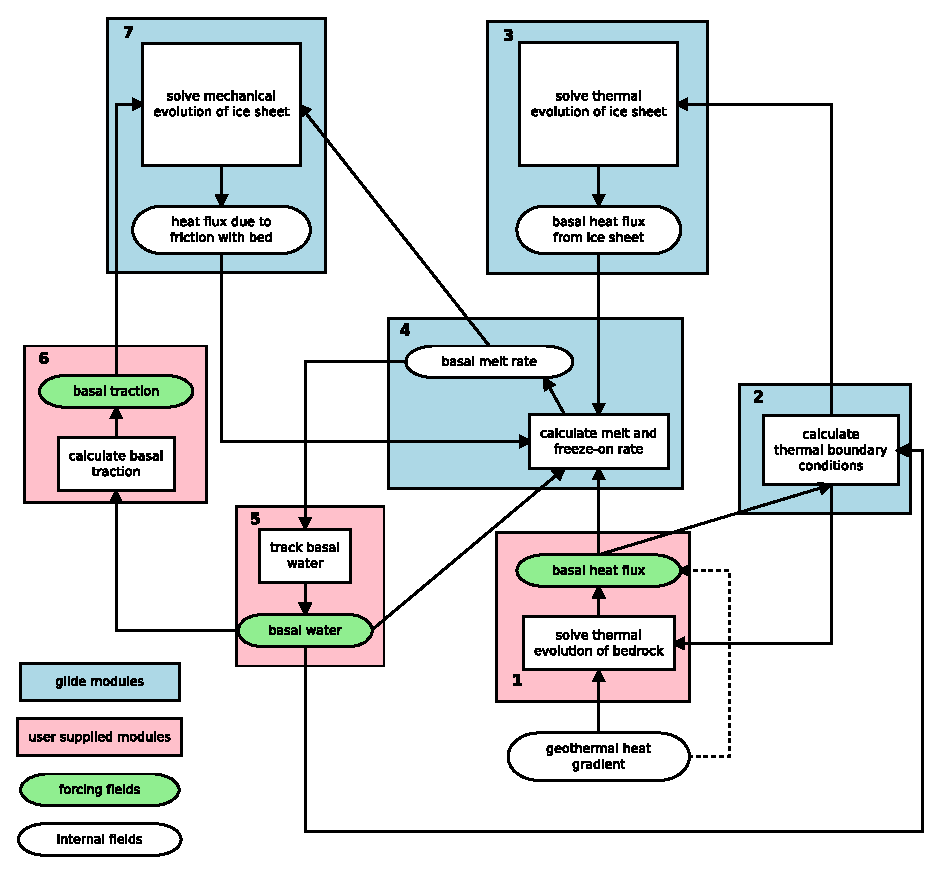
\includegraphics[width=\textwidth]{\dir/figs/basal_alg.eps}
  \caption{Flow diagram illustrating how the various modules communicate with each other by exchanging data fields.}
  \label{num.fig.bc_flow}
\end{figure}
The order of executions is then:
\begin{enumerate}
\item Find the basal heat flux by either solving the equation describing the thermal evolution of the lithosphere, \eqref{num.eq.diffu_rock}, or by using the geothermal heat flux directly. The upper boundary condition of \eqref{num.eq.diffu_rock} is the same as the lower boundary condition of the thermal evolution of the ice sheet.
\item Either (1) the lower boundary condition for the thermal evolution of the ice sheet is given by the basal heat flux from \emph{Step 1}; or (2) if melt water is present, the basal temperature is set to the pressure melting point of ice.
\item Calculate the temperature distribution within the ice sheet given the boundary condition found during \emph{Step 2} and the atmospheric BC.
\item Calculate a melt/freeze--on rate using Equation \eqref{bc.eq.meltrate} given the outgoing heat flux calculated during \emph{Step 3}, friction with the bed (calculated during the previous \emph{Step 7}) and the incoming heat flux from \emph{Step 1}. Freezing occurs only when there is basal water.
\item Track basal water. This is a user supplied module which can take any complexity. Inputs will typically be the melt/freeze--on rate determined during \emph{Step 4}.
\item Calculate the basal traction parameter. Again, this is a user supplied module which typically will involve the presence of basal water (calculated during \emph{Step 5}).
\item Solve the mechanical ice equations given basal traction parameter from \emph{Step 6}.
\end{enumerate}
Clearly, this scheme has the problem that heat is lost if the basal heat flux is such that more water could be frozen than is available. This might be avoided by iterating the process. On the other hand, the heat loss may be negligible if time steps are fairly small.

\section{Isostatic Adjustment}
The ice sheet model includes simple approximations for calculating isostatic adjustment. These approximations depend on how the lithosphere and the mantle are treated. For each subsystem there are two models. The lithosphere can be described as a
\begin{description}
\item[\textbf{local lithosphere:}] the flexural rigidity of the lithosphere is ignored, i.e. this is equivalent to ice floating directly on the asthenosphere;
\item[\textbf{elastic lithosphere:}] the flexural rigidity is taken into account;
\end{description}
while the mantle is treated as a
\begin{description}
\item [\textbf{fluid mantle:}] the mantle behaves like a non-viscous fluid, isostatic equilibrium is reached instantaneously;
\item [\textbf{relaxing mantle:}] the flow within the mantle is approximated by an exponentially decaying hydrostatic response function, i.e. the mantle is treated as a viscous half space.
\end{description}

\subsection{Calculation of ice-water load}
At each isostasy time-step, the load of ice and water is calculated, as an
equivalent mantle-depth ($L$). If the basal elevation is above sea-level, then the
load is simply due to the ice:
\begin{equation}
L=\frac{\rho_i}{\rho_m}H,
\label{load_land_ice}
\end{equation}
where $H$ is the ice thickness, with $\rho_i$ and $\rho_m$ being the densities
of the ice and mantle respectively. In the case where the bedrock is below
sea-level, the load is calculated is that due to a change in sea-level rise and/or
the presence of non-floating ice. When the ice is floating ($\rho_i
H<\rho_o(z_0-h)$), the load is only due to sea-level changes
\begin{equation}
L=\frac{\rho_o}{\rho_m}z_0,
\label{load_sea_float}
\end{equation}
whereas when the ice is grounded, it displaces the water, and adds an
additional load:
\begin{equation}
L=\frac{\rho_i H+\rho_o b_r}{\rho_m}.
\label{load_sea_grounded}
\end{equation}
here, $\rho_o$ is the density of sea water, $z_0$ is the change in sea-level
relative to a reference level and $b_r$ is the bedrock elevation relative to the
same reference level. The value of $b_r$ will be negative for submerged bedrock,
hence the plus sign in (\ref{load_sea_grounded}).

\subsection{Elastic lithosphere model}
This is model is selected by setting \texttt{lithosphere = 1} in the
configuration file. By simulatuing the deformation of the lithosphere, the
deformation seen by the aesthenosphere beneath is calculated. In the absence of this
model, the deformation is that due to Archimedes' Principle, as though the
load were floating on the aesthenosphere.

The elastic lithosphere model is based on work by \cite{Lambeck1980}, and its
implementation is fully described in \cite{Hagdorn2003}. The lithosphere
model only affects the geometry of the deformation --- the timescale for
isostatic adjustment is controlled by the aesthenosphere model. 

The load due to a single (rectangular) grid point is approximated as being
applied to a disc of the same area. The deformation due to a disc of ice of
radius $A$ and thickness $H$ is given by these expressions. For $r<A$:
\begin{equation} 
w(r)=\frac{\rho_i H}{\rho_m}\left[1+C_1\,\mathrm{Ber}\left(\frac{r}{L_r}\right)+C_2\,\mathrm{Bei}\left(\frac{r}{L_r}\right)\right],
\end{equation}
and for $r\geq A$:
\begin{equation}
w(r)=\frac{\rho_i
  H}{\rho_m}\left[D_1\,\mathrm{Ber}\left(\frac{r}{L_r}\right)+D_2\,\mathrm{Bei}\left(\frac{r}{L_r}\right)
+D_3\,\mathrm{Ker}\left(\frac{r}{L_r}\right)+D_4\,\mathrm{Kei}\left(\frac{r}{L_r}\right)\right],
\end{equation}
where $\mathrm{Ber}(x)$, $\mathrm{Bei}(x)$, $\mathrm{Ker}(x)$ and
$\mathrm{Kei}(x)$ are Kelvin functions of zero order, $L_r=(D/\rho_m
g))^{1/4}$ is the radius of relative stiffness, and $D$ is the flexural
rigidity. The constants $C_i$ and $D_i$ are given by
\begin{equation}
\begin{array}{rcl}
C_1&=&a\,\mathrm{Ker}'(a)\\
C_2&=&-a\,\mathrm{Ker}'(a)\\
D_1&=&0\\
D_2&=&0\\
D_3&=&a\,\mathrm{Ber}'(a)\\
D_4&=&-a\,\mathrm{Ber}'(a).
\end{array}
\end{equation}
Here, the prime indicates the first spatial derivative of the Kelvin functions.

\subsection{Relaxing aesthenosphere model}
If a fluid mantle is selected, it adjusts instantly to changes in lithospheric
loading. However, a relaxing mantle is also available.

%%% Local Variables: 
%%% mode: latex
%%% TeX-master: "isos"
%%% End: 



\chapter{Higher-Order Ice Dynamics - Glissade Dynamical Core}
\renewcommand{\dir}{higher-order}

\section{Higher-Order Dynamics in CISM}
\label{sc:higher-order-into}

\subsection{Basics}
The main distinction between so-called higher-order models and 0-order (or ``shallow ice") models is that higher-order models attempt a closer approximation to solving the non-linear Stokes equations. In general, this usually means incorporating some approximation of horizontal-stress gradients (along-flow stretching or compression and across-flow shearing) in addition to the vertical stress gradients that are accounted for in shallow ice models (Figure \ref{fig:stressbalance}). This is important for several reasons:

\begin{figure}
  \begin{center}
    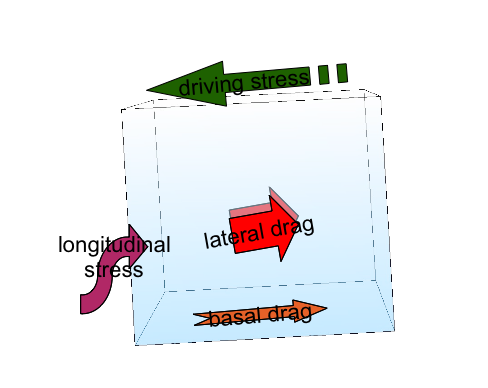
\includegraphics[width=0.5\columnwidth]{\dir/figs/StressBalance.eps}
  \end{center}
  \caption{The gravitational stress available to move the ice is the driving stress, indicated in green. Because the ice is assumed to be in equilibrium, the sum of the other stresses is equal to (i.e., must balance) the gravitational driving stress. In the 0-order model (shallow-ice approximation) the driving stress is assumed to be balanced by basal drag alone. In higher-order models, this restriction is relaxed and the balance of stresses now includes lateral and/or longitudinal stresses. Because these stresses must be computed based on conditions outside the local ice column, the model becomes significantly more complex.}
  \label{fig:stressbalance}
\end{figure} 

\begin{itemize}
\item For the ice-sheet regions of greatest interest -- e.g. ice streams, ice shelves, and other regions of fast flow -- horizontal-stress gradients are at least as important as vertical stress gradients. To model the flow in these regions accurately, higher-order models are required.

\item The shallow-ice approximation, applied to situations in which there is basal sliding, gives rise to a singularity in the the vertical velocity. Models compute the vertical velocity by integrating the incompressibility equation:

\begin{equation}
  \label{ho.eq.incompress}
  \frac{\partial w}{\partial z} = -\frac{\partial u}{\partial x}-\frac{\partial v}{\partial y}.
\end{equation}

If there is a jump 
from no sliding in one grid cell to sliding in an adjacent cell, the horizontal velocity gradients at the bed will depend on the grid spacing; the horizontal gradients (and through incompressibility, the vertical velocity gradient and thus the vertical velocity) will become increasingly large as the grid spacing decreases. Obviously, this should be avoided.

\item Incomplete knowledge of the stresses near the grounding line, which are often dominated by horizontal rather than vertical stresses, makes it unlikely that shallow ice models will ever be able to accurately simulate grounding line advance and retreat.

\item In some regions of very slow flow, like ice divides, horizontal-stress gradients are important or dominant. Ice cores are often recovered at ice divides, and flow modeling is important for interpreting ice core records and using information (such as layer thickness) to infer the past flow history in the region. In order to model that flow correctly, one must include horizontal stresses. (At an ice divide the surface slope is \(\sim\)0, in which case vertical stress gradients that drive deformation in 0-order models are also \(\sim\)0. In reality, deformation is not 0 at ice divides, but is controlled by horizontal stretching rather than vertical shearing).
\end{itemize}

The term ``higher-order'' comes from scaling analyses of the Stokes equations for which a scaling parameter $\lambda=H/L$ (the ratio of the thickness to the horizontal length scale of interest) is used to assign importance to the various terms. Shallow ice models retain only terms of order 0 while higher-order models also retain terms of order 1 (and possibly more) (Figure \ref{fig:hoeqns}). 

\begin{figure}
  \begin{center}
    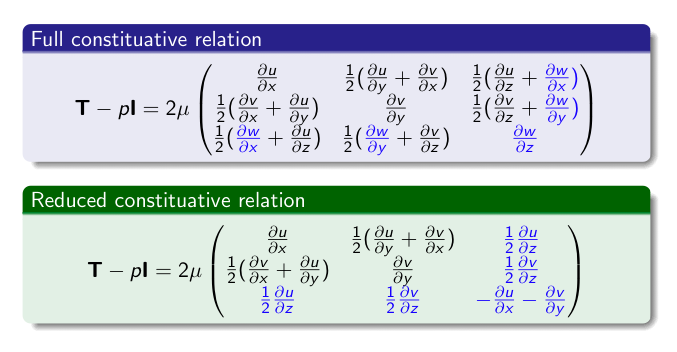
\includegraphics[width=0.7\columnwidth]{\dir/figs/HOeqns.eps}
   \end{center}
  \caption{Stokes-flow (top) and first-order (bottom) constitutive equations. \textit{WHL: ``constitutive'' is misspelled above.}}
  \label{fig:hoeqns}
\end{figure} 

\subsection{Available schemes}

\begin{itemize}
\item The most fundamental higher-order scheme is the full set of nonlinear Stokes equations. Because of the computational burden, many large-scale 3d models solve lower-order approximations of the Stokes equations (Figure \ref{fig:phylogeny}). However, several groups have made significant advances in Stokes modeling
(e.g. the ELMER-Ice effort; \citet{gagliardini:2013iv}). 
Current DOE-funded efforts include implementation of a nonlinear Stokes model on unstructured grids \citep{Leng:2012ia}.
\end{itemize}

\begin{itemize}
\item \textit{WHL: Is the SSA truly a higher-order approximation?}
Probably the most long-lived higher-order approximation in glaciology is the shallow-shelf approximation (or SSA) describing flow within an ice shelf (or ice stream if non-zero basal drag is included). The SSA was developed and made popular by Douglas MacAyeal (e.g., \citet{Macayeal:1989uo}). 
Its main disadvantage is that it is not fully 3d, as it assumes uniform velocity throughout the ice thickness driven only by horizontal stress gradients. It is, however, adequate for describing fast flow in many parts of ice sheets, such as ice shelves and some ice streams. In these regions, not resolving vertical gradients is a computational advantage.   
\end{itemize}

\begin{itemize}
\item The SSA equations are actually a depth-averaged form of a more general higher-order model, commonly referred to as the ``Blatter-Pattyn model" (\citet{BLATTER:1995wz}; \citet{Pattyn:2003tj}). 
Blatter-Pattyn dynamics, synonymous with and more formally described as the ``first-order accurate Stokes approximation"\footnote{See \citet{Schoof:2010dl} and \citet{DUKOWICZ:2010wb} for a more complete scaling analysis and derivation of the first-order Stokes approximation.}, are currently implemented in CISM's default higher-order dynamical core.
\textit{WHL: Should we distinguish Blatter-Pattyn from L1L2, which also is formally first-order accurate? Should there be a following item on L1L2?}
\end{itemize}

\begin{itemize}
\item Several hybrid schemes exist that are computationally cheaper than the Blatter-Pattyn model. These combine solutions to the shallow ice approximation (for resolving vertical gradients) and the SSA approximation (for resolving horizontal gradients) so that a fully 3d solution is obtained. 
%It isn't yet known how well these model solutions compare to fully 3d models, or if one approach (hybrid vs. fully 3d solution) is superior to the other. 
David Pollard of Penn State and Ed Bueler of Univ. of Alaska Fairbanks have developed large-scale models using distinct hybrid approaches (\citet{Bueler:2009ee}; \citet{Pollard:2009ed}).
\end{itemize}

A review paper by \citet{Schoof:2013is} goes into a fair amount of detail about the various ice flow modeling approximations, their derivations, and their applicability.

\subsection{Shallow-ice vs. higher-order models: practical differences}

\begin{figure}
  \begin{center}
    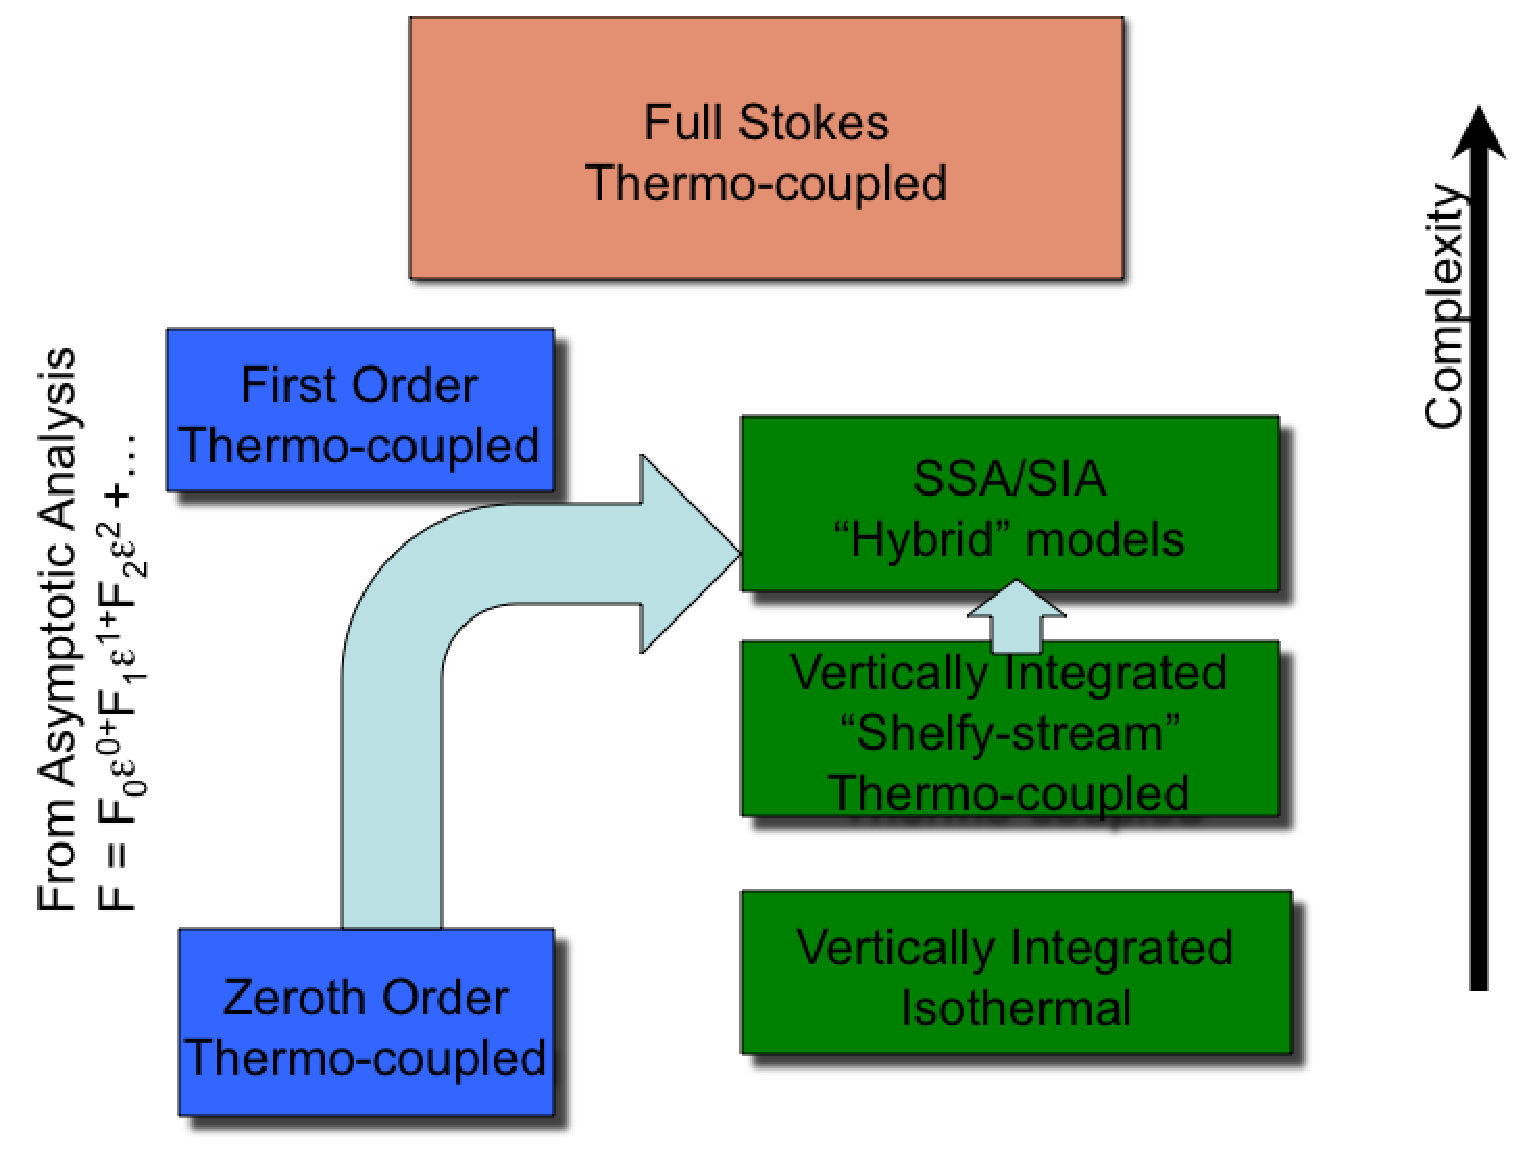
\includegraphics[width=0.5\columnwidth]{\dir/figs/ISMPhylogeny.eps}
   \end{center}
  \caption{The relationship between several common varieties of ice sheet modesl. Complexity increases along the vertical axis.}
   \label{fig:phylogeny}
\end{figure} 

There are large differences between shallow-ice and higher-order models in 
\textbf{(1)} how the momentum equations (the dynamics, or stress balance) are solved and 
\textbf{(2)} how the information derived from that solution (the kinematics, or velocity fields) is used to evolve the ice sheet geometry in time. There are two main reasons for these differences:

\begin{itemize}
\item  The numerical solution of the dynamical equations is fundamentally different. For the shallow ice case, we need only local information (surface elevation and thickness) to solve for the velocity as a function of depth in a single column of ice. We do this pointwise for each location on the model domain (in map view), which is a relatively easy numerical problem.  Each column of velocities leads to a tridiagonal matrix that is easy to invert (to solve for the velocities). This problem is $embarrassingly$ $parallel$, since each column of unknown velocities results in a tridiagonal matrix that can be solved on a single processor. For higher-order models, however, the solution at any point also depends on the solution at neighboring points (in map view),
leading to an elliptic system of equations in which every velocity must be solved for simultaneously with every other velocity. The result is a much larger system of equations, which are more difficult to solve on one processor and far more difficult to solve on multiple processors. Because large-scale higher-order model applications (e.g., whole-ice-sheet models) require efficient, robust solution and parallelization techniques, this is an active area of current research.  
\end{itemize}

\begin{itemize}
\item  The equations governing dynamics AND evolution in a shallow-ice model can be recast as a nonlinear diffusion equation for ice thickness. A single system of equations is solved to calculate the velocity field and evolve the ice sheet geometry. For higher-order models, we must first solve the momentum balance equations to obtain the velocity field, and then use some other scheme to evolve the ice thickness. 
\end{itemize}

These differences imply that a higher-order model must be built in a fundamentally different way than a shallow-ice model.
Most recent development work on CISM has focused on higher-order dynamics.

%The equations describing a (2d) higher-order flow that is vertically integrated (i.e., the SSA) are:
%
%\begin{align*}
%\frac{\partial}{\partial x}\left ( 2 \eta H 
%\left(2\frac{\partial u}{\partial x}+\frac{\partial v}{\partial y}\right)\right)
%+\frac{\partial}{\partial y}\left(\eta H\left(
%\frac{\partial u}{\partial y}+\frac{\partial v}{\partial x}\right)\right)
%=\rho_w gH \frac{\partial s}{\partial x}
%\end{align*}
%
%
%\begin{align*}
%\frac{\partial}{\partial y}\left ( 2 \eta H 
%\left(2\frac{\partial v}{\partial y}+\frac{\partial u}{\partial x}\right)\right)
%+\frac{\partial}{\partial x}\left(\eta H\left(
%\frac{\partial u}{\partial y}+\frac{\partial v}{\partial x}\right)\right)
%=\rho_w gH \frac{\partial s}{\partial y}
%\end{align*}

The equations describing a (3d) higher-order flow\footnote{Specifically, the first-order accurate Stokes approximation discussed above. These will be derived in more detail in Section \ref{sc:higher-order-mom}.} are:

\begin{equation}
  \begin{split}
  & x: \frac{\partial}{\partial x}\left ( 2 \eta  
\left(2\frac{\partial u}{\partial x}+\frac{\partial v}{\partial y}\right)\right)
+\frac{\partial}{\partial y}\left(\eta \left(
\frac{\partial u}{\partial y}+\frac{\partial v}{\partial x}\right)\right)
+\frac{\partial}{\partial z}\left(\eta \frac{\partial u}{\partial z}\right)
=\rho_i g \frac{\partial s}{\partial x} \\
  & y: \frac{\partial}{\partial y}\left ( 2 \eta 
\left(2\frac{\partial v}{\partial y}+\frac{\partial u}{\partial x}\right)\right)
+\frac{\partial}{\partial x}\left(\eta \left(
\frac{\partial u}{\partial y}+\frac{\partial v}{\partial x}\right)\right)
+\frac{\partial}{\partial z}\left(\eta \frac{\partial v}{\partial z}\right)
=\rho_i g \frac{\partial s}{\partial y} \\
  \end{split}
\end{equation}

\textit{WHL: Since the constitutive law hasn't been introduced yet, I wonder if these equations should be written in terms
of $\tau$ instead of strain rates. Also, do any symbols need to be defined?}
In these equations we can point out several important differences between shallow-ice and higher-order models: 
\begin{enumerate}
%\item  The vertically integrated model includes the ice thickness, $H$, in each term. This is a reflection of the integration and does not appear in the first-order equations.
%\item  Accounting for the thickness not appearing, the only other difference is the presence of a vertical diffusion of horizontal velocities. This is the the third term on the left in the above equations.
\item  The third term on the left-hand side represents the vertical diffusion of horizontal velocities. In a shallow-ice model, this term alone accounts for all ice dynamics and balances the entire body force in the $x$ direction (the term on the right-hand side). Since the velocity gradients are only in the vertical direction, the solution is local (in map view).

\item  The first-order equations must be solved for each of a set of horizontal layers (the number of which is defined by the resolution in the vertical, here $dz$). These layers communicate with each other through the vertical diffusion term.

\item  The first and second sets of terms on the left-hand side represent the resistance to the body-force term that result from ``membrane stresses" (i.e., stresses arising from horizontal velocity gradients). These horizontal gradients make the problem elliptic and non-local. The absence of membrane stresses in the shallow-ice momentum balance is the primary reason for their failure to realistically simulate the flow in outlet glaciers, ice streams, and ice shelves.

\end{enumerate}

%Both sets of equations are non-linear elliptical equations and much of the same technology can be used solve them. 
Other complications arise when we account for boundary conditions at the lateral margins of the domain and at the upper and lower ice surfaces. We describe both the governing equations and the boundary conditions in more detail below.
% (note that for the vertically integrated flow, there are no explicit boundary conditions for the upper and lower surfaces; they are accounted for and incorporated during the vertical integration).

%\subsection{Higher-order CISM}

%A very useful higher-order model intercomparison project (ISMIP-HOM) was organized by Frank Pattyn from the Université Libre de Bruxelles. That project, which resulted in a set of "benchmark" experiments for higher-order models, is reported on formally in Pattyn et al. (2008). 


\section{Higher-Order Momentum Balance}
\label{sc:higher-order-mom}

\begin{figure}
  \begin{center}
    
\includegraphics[width=0.65\columnwidth]{\dir/figs/GIS.eps}
   \end{center}
  \caption{Observation-based balance velocities for Greenland (left) and depth-averaged speed from higher-order CISM (right) with basal sliding coefficients optimized to match the balance velocities (after Price et al., $PNAS$, \textbf{108}(22), 2011).}
  \label{fig:GIS_PNAS}
\end{figure} 

The higher-order dynamics scheme currently implemented in CISM (some output from which is shown in Figure \ref{fig:GIS_PNAS}) is discussed in more detail in the following sections. First, the derivation of the equations themselves is discussed, followed by a discussion and derivation of the boundary conditions. Generic solution methods for the nonlinear system of equations are then discussed. Finally, there is a brief discussion on the solution of the thickness evolution equation, which as noted above requires a different approach than in shallow-ice models.

\subsection{Derivation of the Blatter-Pattyn Equations}

The higher-order dynamics scheme implemented in CISM is based on the 1st-order accurate Stokes approximation (also often referred to as the ``Blatter-Pattyn" model). The starting point for this model is the full, nonlinear Stokes equations given by

\begin{align*}
  & x:\quad \frac{\partial \tau _{xx}}{\partial x}-\frac{\partial P}{\partial x}+\frac{\partial \tau _{xy}}{\partial y}+\frac{\partial \tau _{xz}}{\partial z}=0 \\ 
 & y:\quad \frac{\partial \tau _{yy}}{\partial y}-\frac{\partial P}{\partial y}+\frac{\partial \tau _{xy}}{\partial x}+\frac{\partial \tau _{yz}}{\partial z}=0 \\ 
 & z:\quad \frac{\partial \tau _{zz}}{\partial z}-\frac{\partial P}{\partial z}+\frac{\partial \tau _{zy}}{\partial y}+\frac{\partial \tau _{xz}}{\partial x}=\rho g, \\ 
\end{align*}

where \textit{P} is the pressure and {\large \(\tau{}\)} is the deviatoric stress tensor. The latter is given by $\tau _{ij}=\sigma _{ij}+P\delta _{ij}$, 
where {\large \(\sigma{}\)} is the full stress tensor.

There are a number of ways to argue that, due to the shallowness of ice sheets (because the ratio of \textit{H}/\textit{L}, where \textit{H} is the thickness and \textit{L} is a relevant horizontal length scale, is small), the equations above can be reduced to the following first-order approximation:

\begin{align*}
  & x:\quad \frac{\partial \tau _{xx}}{\partial x}-\frac{\partial P}{\partial x}+\frac{\partial \tau _{xy}}{\partial y}+\frac{\partial \tau _{xz}}{\partial z}=0 \\ 
 & y:\quad \frac{\partial \tau _{yy}}{\partial y}-\frac{\partial P}{\partial y}+\frac{\partial \tau _{xy}}{\partial x}+\frac{\partial \tau _{yz}}{\partial z}=0 \\ 
 & z:\quad \frac{\partial \tau _{zz}}{\partial z}-\frac{\partial P}{\partial z}=\rho g \\ 
\end{align*}

The arguments that support this reduction are fairly complex, either based on a variational analysis or an asymptotic analysis. \citet{Schoof:2010dl} and \citet{DUKOWICZ:2010wb} provide more details on the mathematical background that allows us to state that these equations are first-order accurate approximations to the Stokes equations. 

We continue by noting that the 3rd (vertical) balance equation above can be integrated through the depth of the ice sheet to give an expression for the pressure, $P=\rho g\left( s-z \right)+\tau _{zz}(z)$. This is simply a statement the the full vertical normal stress is balanced by the hydrostatic pressure (the so-called \textit{hydrostatic assumption}). This expression can be substituted into the horizontal pressure gradient terms above to remove pressure from the equations. For example, for the \textit{x} component of velocity we have

\begin{align*}
  & x:\quad \frac{\partial \tau _{xx}}{\partial x}+\frac{\partial \tau _{xy}}{\partial y}+\frac{\partial \tau _{xz}}{\partial z}=\frac{\partial P}{\partial x} \\ 
 & x:\quad \frac{\partial \tau _{xx}}{\partial x}+\frac{\partial \tau _{xy}}{\partial y}+\frac{\partial \tau _{xz}}{\partial z}=\frac{\partial }{\partial x}\left[ \rho g\left( s-z \right)+\tau _{zz}(z) \right] \\ 
 & x:\quad \frac{\partial \tau _{xx}}{\partial x}-\frac{\partial \tau _{zz}}{\partial x}+\frac{\partial \tau _{xy}}{\partial y}+\frac{\partial \tau _{xz}}{\partial z}=\rho g\frac{\partial s}{\partial x} \\ 
\end{align*}

Now we can use the incompressibility and stress-strain colinearity constraints to rewrite the vertical normal deviatoric stress in terms of horizontal normal deviatoric stresses,

\begin{align*}
  & \tau _{zz}=-\tau _{xx}-\tau _{yy} \text{             ... taking gradients with respect to $x$ ... } \\ 
 & -\frac{\partial \tau _{zz}}{\partial x}=-\frac{\partial }{\partial x}\left( -\tau _{xx}-\tau _{yy} \right)=\frac{\partial \tau _{xx}}{\partial x}+\frac{\partial \tau _{yy}}{\partial x}.  \\
\end{align*}
 
Substituting this expression for the $x$ derivative of the vertical normal deviatoric stress back into our horizontal stress balance equation above we obtain,
 
\begin{align*}
 & \frac{\partial \tau _{xx}}{\partial x}-\frac{\partial \tau _{zz}}{\partial x}+\frac{\partial \tau _{xy}}{\partial y}+\frac{\partial \tau _{xz}}{\partial z}=\rho g\frac{\partial s}{\partial x}\quad \text{    ... becomes ... } \\
 & 2\frac{\partial \tau _{xx}}{\partial x}+\frac{\partial \tau _{yy}}{\partial x}+\frac{\partial \tau _{xy}}{\partial y}+\frac{\partial \tau _{xz}}{\partial z}=\rho g\frac{\partial s}{\partial x}\quad. \\
\end{align*}

Note that at this point we have removed the vertical balance equation entirely; it has been incorporated into the horizontal balance equations through incompressibility. The horizontal balance equations are now: 

\begin{align*}
  & x:\quad 2\frac{\partial \tau _{xx}}{\partial x}+\frac{\partial \tau _{yy}}{\partial x}+\frac{\partial \tau _{xy}}{\partial y}+\frac{\partial \tau _{xz}}{\partial z}=\rho g\frac{\partial s}{\partial x}\quad,  \\ 
 & y:\quad 2\frac{\partial \tau _{yy}}{\partial y}+\frac{\partial \tau _{xx}}{\partial y}+\frac{\partial \tau _{xy}}{\partial x}+\frac{\partial \tau _{yz}}{\partial z}=\rho g\frac{\partial s}{\partial y}. \\
\end{align*}

Next, we want to write these equations in terms of velocities, since that is what we are ultimately solving for. The link between stresses  and velocities is through the constitutive law for ice (here we assume Nye's generalization of Glen's law) -- relating strain rates to stresses -- and the definition of the strain rate tensor -- relating strain rates to velocity gradients.

\begin{align*}
  & 1.\quad \tau _{ij}=B\dot{\varepsilon }_{e}^{\frac{1-n}{n}}\dot{\varepsilon }_{ij},\quad B=B(T) \\ 
 & 2.\quad \dot{\varepsilon }_{ij}=\frac{1}{2}\left( \frac{\partial u_{i}}{\partial x_{j}}+\frac{\partial u_{j}}{\partial x_{i}} \right) \\ 
 & 3.\quad 2\dot{\varepsilon }_{e}=\dot{\varepsilon }_{ij}\dot{\varepsilon }_{ij} \\ 
 & 4.\quad \eta \equiv \frac{1}{2}B\dot{\varepsilon }_{e}^{\frac{1-n}{n}} \\ 
 & 5.\quad \tau _{ij}=2\eta \dot{\varepsilon }_{ij} \\ 
\end{align*}

In order, the four expressions above give: 

\begin{enumerate}
\item  Glen's flow law\footnote{Technically, we are using the \textit{inverse} form of the flow-law here.}, where $B(T) = A(T)^{\frac{1-n}{n}}$ is the temperature dependent rate factor
\item  The definition of the strain-rate tensor in terms of velocity gradients
\item  The definition of the effective strain rate, $\dot{\varepsilon }_{e}$, a norm of the strain-rate tensor
\item  A definition for the ``effective viscosity" (after rearranging some terms in (1))
\item  Items (1)-(4) allow us to write the relationship between stress and strain in a standard ``Newtonian" way, but with a non-Newtonian (nonlinear) viscosity
\end{enumerate}

Now, taking these definitions into our stress balance equations above and expanding in terms of strain rates, velocity gradients, and the effective viscosity, we have (for the \textit{x} direction only):

\begin{align*}
  & x:\quad 2\frac{\partial \tau _{xx}}{\partial x}+\frac{\partial \tau _{yy}}{\partial x}+\frac{\partial \tau _{xy}}{\partial y}+\frac{\partial \tau _{xz}}{\partial z}=\rho g\frac{\partial s}{\partial x}, \\ 
 & x:\quad 2\frac{\partial }{\partial x}\left( 2\eta \dot{\varepsilon }_{xx} \right)+\frac{\partial }{\partial x}\left( 2\eta \dot{\varepsilon }_{yy} \right)+\frac{\partial }{\partial y}\left( 2\eta \dot{\varepsilon }_{xy} \right)+\frac{\partial }{\partial z}\left( 2\eta \dot{\varepsilon }_{xz} \right)=\rho g\frac{\partial s}{\partial x}, \\ 
 & x:\quad 4\frac{\partial }{\partial x}\left( \eta \frac{\partial u}{\partial x} \right)+2\frac{\partial }{\partial x}\left( \eta \frac{\partial v}{\partial y} \right)+\frac{\partial }{\partial y}\left[ \eta \left( \frac{\partial u}{\partial y}+\frac{\partial v}{\partial x} \right) \right]+\frac{\partial }{\partial z}\left( \eta \frac{\partial u}{\partial z} \right)=\rho g\frac{\partial s}{\partial x}. \\ 
\end{align*}

An analogous expression describes the \textit{y} direction momentum balance equation. 
%For actually solving the system of equations, it is advantageous to combine all \textit{v} gradient terms for the \textit{x} balance equation and move them to the right-hand side (and vice versa for the \textit{y} balance equation). 
Thus, the final form of the equations to be discretized and solved is given by:

\begin{align*}
  & x:\quad 4\frac{\partial }{\partial x}\left( \eta \frac{\partial u}{\partial x} \right)+\frac{\partial }{\partial y}\left( \eta \frac{\partial u}{\partial y} \right)
  +2\frac{\partial }{\partial x}\left( \eta \frac{\partial v}{\partial y} \right)+\frac{\partial }{\partial y}\left( \eta \frac{\partial v}{\partial x} \right)
  +\frac{\partial }{\partial z}\left( \eta \frac{\partial u}{\partial z} \right)=\rho g\frac{\partial s}{\partial x}, \\ 
 & y:\quad 4\frac{\partial }{\partial y}\left( \eta \frac{\partial v}{\partial y} \right)+\frac{\partial }{\partial x}\left( \eta \frac{\partial v}{\partial x} \right)
 +2\frac{\partial }{\partial y}\left( \eta \frac{\partial u}{\partial x} \right)+\frac{\partial }{\partial x}\left( \eta \frac{\partial u}{\partial y} \right)
 +\frac{\partial }{\partial z}\left( \eta \frac{\partial v}{\partial z} \right)=\rho g\frac{\partial s}{\partial y}. \\ 
\end{align*}

%\documentclass[a4paper,12pt]{article}
%\usepackage[english]{babel} % Quotes won't work without babel
%\usepackage[utf8]{inputenc}  % This is very important!
%\usepackage[T1]{fontenc}
%
%\usepackage[pdfborder={0 0 0}, breaklinks=true, pdftex=true, raiselinks=true]{hyperref}
%\usepackage{graphicx}
%
%\usepackage{amsmath}
%
%\title{Higher-Order Model Boundary Conditions}
%\date{}
%
%\begin{document}
%\maketitle

\section{Higher-Order Model Boundary Conditions}

We will go through an approximate derivation of the boundary conditions that are implemented with CISM's higher-order scheme. By approximate we mean that some of the derivation is guided by physical intuition and reasonable arguments, rather than through the application of rigorous mathematics. In the end, we wind up with the same set of equations that one ends up using the more rigorous approach (see, e.g. \textit{Dukowicz et al., J. Glaciol.}, 56(197), 2010). We will look at the derivation in three parts, (1) the free surface boundary condition, (2) the specified basal traction boundary condition, and (3) lateral boundary conditions.

\subsection{Stress Free Surface}
At the ice surface, a stress-free boundary condition is applied. The traction vector, \textit{{\large T}}, must be continuous at the ice sheet surface and, assuming that atmospheric pressure and surface tension are small, we have

\begin{align*}
 & T_{i}=-T_{i(boundary)}\approx 0 \\ 
 & T_{i}=\sigma _{ij}n_{j}=\sigma _{i1}n_{1}+\sigma _{i2}n_{2}+\sigma _{i3}n_{3}=0\\
\end{align*}

where the $n_i$ are the components of the outward facing, unit normal vector in Cartesisan coordinates.

For a function \textit{F(x,y,z) = z -- f(x,y) = 0}, where \textit{z = f(x,y)} defines the surface, the gradient of \textit{F(x,y,z)} gives the components of the surface normal vector.

For the case of the ice sheet surface, $s = f(x,y)$ and the surface normal is given by

\begin{align*}
n_{i}=\left( -\frac{\partial s}{\partial x},-\frac{\partial s}{\partial y},1 \right)\frac{1}{a}
\end{align*}

where

\begin{align*}
a=\sqrt{\left( \frac{\partial f}{\partial x} \right)^{2}+\left( \frac{\partial f}{\partial y} \right)^{2}+1^{2}}.
\end{align*}

The expression above for $T_i$ gives three equations that must be satisfied for a free surface boundary condition:

\begin{align*}
  & i=x:\quad T_{x}=\sigma _{xx}n_{x}+\sigma _{xy}n_{y}+\sigma _{xz}n_{z}=0, \\ 
 & i=y:\quad T_{y}=\sigma _{yx}n_{x}+\sigma _{yy}n_{y}+\sigma _{yz}n_{z}=0, \\ 
 & i=z:\quad T_{z}=\sigma _{zx}n_{x}+\sigma _{zy}n_{y}+\sigma _{zz}n_{z}=0. \\ 
\end{align*}

Expanding the last one and expressing stresses in terms of strain rates and pressures, where $\eta$ is the effective viscosity, gives

\begin{align*}
\left( 2\eta \dot{\varepsilon }_{zx} \right)n_{x}+\left( 2\eta \dot{\varepsilon }_{zy} \right)n_{y}+\left( 2\eta \dot{\varepsilon }_{zz}-P \right)n_{z}=0,
\end{align*}

which, when solved for the pressure gives

\begin{align*}
Pn_{z}=\left( 2\eta \dot{\varepsilon }_{zz} \right)n_{z}+\left( 2\eta \dot{\varepsilon }_{zx} \right)n_{x}+\left( 2\eta \dot{\varepsilon }_{zy} \right)n_{y}.
\end{align*}


Expanding the above expression in terms of velocity gradients and normal vector components we have

\begin{align*}
P=2\eta \frac{\partial w}{\partial z}-\left( \eta \frac{\partial u}{\partial z} \right)\frac{\partial s}{\partial x}-\left( \eta \frac{\partial v}{\partial z} \right)\frac{\partial s}{\partial y}
\end{align*}

where we have made the usual 1st-order approximation that 

\begin{align*}
\frac{\partial w}{\partial x}=\frac{\partial w}{\partial y}\approx 0.
\end{align*}

Now we use this expression for the pressure and expand the two horizontal boundary condition expressions

\begin{align*}
  & i=x:\quad T_{x}=\sigma _{xx}n_{x}+\sigma _{xy}n_{y}+\sigma _{xz}n_{z}=0, \\ 
 & i=y:\quad T_{y}=\sigma _{yx}n_{x}+\sigma _{yy}n_{y}+\sigma _{yz}n_{z}=0, \\
 \end{align*}

in terms of velocity gradients and the effective viscosity to obtain

\begin{align*}
   {} & \hat{x}:\quad -2\eta \frac{\partial u}{\partial x}\frac{\partial s}{\partial x}-\eta \left( \frac{\partial u}{\partial y}+\frac{\partial v}{\partial x} \right)\frac{\partial s}{\partial y}+\eta \frac{\partial u}{\partial z}=  \\
   {} & \quad \quad \quad \quad \quad -2\eta \frac{\partial w}{\partial z}\frac{\partial s}{\partial x}+\eta \frac{\partial u}{\partial z}\left[ \frac{\partial s}{\partial x}\frac{\partial s}{\partial x} \right]+\eta \frac{\partial v}{\partial z}\left[ \frac{\partial s}{\partial y}\frac{\partial s}{\partial x} \right],  \\
\end{align*}

\begin{align*}
   {} & \hat{y}:\quad -2\eta \frac{\partial v}{\partial y}\frac{\partial s}{\partial y}-\eta \left( \frac{\partial u}{\partial y}+\frac{\partial v}{\partial x} \right)\frac{\partial s}{\partial x}+\eta \frac{\partial v}{\partial z}=  \\
   {} & \quad \quad \quad \quad \quad -2\eta \frac{\partial w}{\partial z}\frac{\partial s}{\partial y}+\eta \frac{\partial u}{\partial z}\left[ \frac{\partial s}{\partial x}\frac{\partial s}{\partial y} \right]+\eta \frac{\partial v}{\partial z}\left[ \frac{\partial s}{\partial y}\frac{\partial s}{\partial y} \right].  \\
\end{align*}

In both of these expression, the terms in square brackets are $\sim{0}$ because, as noted above slopes on ice sheets are small (and the slope squared is exceedingly small). From continuity, we also have

\begin{align*}
\frac{\partial w}{\partial z}=-\frac{\partial u}{\partial x}-\frac{\partial v}{\partial y}.
\end{align*}

Using this expression for the normal vertical velocity gradient and removing the terms in square brackets our two horizontal boundary condition expressions become

\begin{align*}
   {} & \hat{x}:\quad -2\eta \frac{\partial u}{\partial x}\frac{\partial s}{\partial x}-\eta \left( \frac{\partial u}{\partial y}+\frac{\partial v}{\partial x} \right)\frac{\partial s}{\partial y}+\eta \frac{\partial u}{\partial z}=2\eta \left( \frac{\partial u}{\partial x}\frac{\partial s}{\partial x}+\frac{\partial v}{\partial y}\frac{\partial s}{\partial x} \right),  \\
   {} & \hat{y}:\quad -2\eta \frac{\partial v}{\partial y}\frac{\partial s}{\partial y}-\eta \left( \frac{\partial u}{\partial y}+\frac{\partial v}{\partial x} \right)\frac{\partial s}{\partial x}+\eta \frac{\partial v}{\partial z}=2\eta \left( \frac{\partial u}{\partial x}\frac{\partial s}{\partial y}+\frac{\partial v}{\partial y}\frac{\partial s}{\partial y} \right).  \\
\end{align*}

As in the derivation of the 1st-order stress balance equations, collect terms of a particular velocity gradient (that is, \textit{u} or \textit{v}) and move them to one side of the equation and, lastly, divide through by the effective viscosity \textit{\(\eta{}\)} to get the final form of the 1st-order free surface boundary conditions

\begin{align*}
   {} & \hat{x}:\quad -4\frac{\partial u}{\partial x}\frac{\partial s}{\partial x}-\frac{\partial u}{\partial y}\frac{\partial s}{\partial y}+\frac{\partial u}{\partial z}=2\frac{\partial v}{\partial y}\frac{\partial s}{\partial x}+\frac{\partial v}{\partial x}\frac{\partial s}{\partial y},  \\
   {} & \hat{y}:\quad -4\frac{\partial v}{\partial y}\frac{\partial s}{\partial y}-\frac{\partial v}{\partial x}\frac{\partial s}{\partial x}+\frac{\partial v}{\partial z}=2\frac{\partial u}{\partial x}\frac{\partial s}{\partial y}+\frac{\partial u}{\partial y}\frac{\partial s}{\partial x}.  \\
\end{align*}

\subsection{Specified Basal Traction}
Derivation of the basal boundary condition follows that above for the free surface except that (1) the right-hand side of the equation is not zero, rather it consists of an assumed basal traction vector with components 
\begin{align*}
\left( \tau _{bx},\tau _{by} \right),
\end{align*}
(2) the outward facing normal vector components now consist of horizontal gradients in the basal surface (with a resulting sign switch on the $x,y,z$ components relative to the upper surface), and (3) the effective viscosity does not disappear from the equations when we divide through. Making these substitutions we obtain the 1st-order basal boundary conditions for a specified basal traction

\begin{align*}
  & \hat{x}:\quad 4\frac{\partial u}{\partial x}\frac{\partial b}{\partial x}+\frac{\partial u}{\partial y}\frac{\partial b}{\partial y}-\frac{\partial u}{\partial z}=-2\frac{\partial v}{\partial y}\frac{\partial b}{\partial x}-\frac{\partial v}{\partial x}\frac{\partial b}{\partial y}+\frac{\tau _{bx}}{\eta }, \\ 
 & \hat{y}:\quad 4\frac{\partial v}{\partial y}\frac{\partial b}{\partial y}+\frac{\partial v}{\partial x}\frac{\partial b}{\partial x}-\frac{\partial v}{\partial z}=-2\frac{\partial u}{\partial x}\frac{\partial b}{\partial y}-\frac{\partial u}{\partial y}\frac{\partial b}{\partial x}+\frac{\tau _{by}}{\eta }. \\
 \end{align*}

We assume that basal traction is related to basal sliding velocity through a traction paramter, $\beta$, such that

\begin{align*}
\tau _{bx}=\left. -\beta u \right|_{z=b},\quad \tau _{by}=\left. -\beta v \right|_{z=b}.
\end{align*}

Note that the negative sign in front of the $\beta$ indicates that the traction vector is oriented parallel and in the opposite direction to the sliding velocity vector.

Substituting this expression into the above gives our final horizontal boundary conditions at the ice sheet base

\begin{align*}
  & \hat{x}:\quad 4\frac{\partial u}{\partial x}\frac{\partial b}{\partial x}+\frac{\partial u}{\partial y}\frac{\partial b}{\partial y}-\frac{\partial u}{\partial z}+\left( \frac{B}{\eta } \right)u=-2\frac{\partial v}{\partial y}\frac{\partial b}{\partial x}-\frac{\partial v}{\partial x}\frac{\partial b}{\partial y}, \\ 
 & \hat{y}:\quad 4\frac{\partial v}{\partial y}\frac{\partial b}{\partial y}+\frac{\partial v}{\partial x}\frac{\partial b}{\partial x}-\frac{\partial v}{\partial z}+\left( \frac{B}{\eta } \right)v=-2\frac{\partial u}{\partial x}\frac{\partial b}{\partial y}-\frac{\partial u}{\partial y}\frac{\partial b}{\partial x}. \\ 
\end{align*}

\subsection{Specified Basal Yield Stress}
The above implementation of a specified basal traction can be altered to simulate sliding over a sediment-covered bed for which the sediment has a plastic rheology. That is, sliding does not occur below the specified yield stress of the underlying material (e.g. a water saturated (thawed) subglacial till). When the yield stress, $\tau_0$ is reached, sliding occurs at a rate that maintains but does not exceed that yield stress. Consider the \textit{x} direction boundary condition above, written out in terms of basal stress components,

\begin{align*}
  & \hat{x}:\quad 4\eta \frac{\partial u}{\partial x}\frac{\partial b}{\partial x}+\eta \frac{\partial u}{\partial y}\frac{\partial b}{\partial y}-\eta \frac{\partial u}{\partial z}=-2\eta \frac{\partial v}{\partial y}\frac{\partial b}{\partial x}-\eta \frac{\partial v}{\partial x}\frac{\partial b}{\partial y}-\tau _{bx}, \\ 
 & \quad \quad \quad \quad \quad \quad \tau _{bx}\approx \tau _{0}=\tau _{0}\left( \frac{u}{\left| \mathbf{u} \right|} \right)=\tau _{0}\left( \frac{u}{\sqrt{u_{0}^{2}+v_{0}^{2}+\gamma }} \right) \\ 
\end{align*}

In the expression above, $u$ is the $x$ component of the basal sliding velocity from the current iteration, $u_0$ and $v_0$ are components from the previous iteration, and $\gamma$ is a regularization constant (a small constant number to avoid division by zero during early iterations). Note that as the solution converges, velocities at the current and previous iteration are nearly equal, and the expression in parentheses approaches 1, in which case the basal stress and yield stress are approximately equal. 

We can easily accommodate this in our earlier framework for incorporating the traction parameter $\beta$ by treating it as nonlinear and dependent on the velocity,

\begin{align*}
  & \tau _{bx}=-\beta u,\quad \quad  \\ 
 & \beta \equiv \frac{\tau _{0}}{\sqrt{u_{0}^{2}+v_{0}^{2}+\gamma }},\quad  \\ 
 & \tau _{bx}=-\left( \frac{\tau _{0}}{\sqrt{u_{0}^{2}+v_{0}^{2}+\gamma }} \right)u.\quad  \\
\end{align*}

Thus, we can implement plastic bed sliding behavior simply by substituting the above expression for our "nonlinear" \textit{{\large \(\beta{}\)}} into our previous expressions for the basal boundary conditions in \textit{x} (a similar expression applies for the \textit{y} direction). The Figures below show some examples of this type of boundary condition for the case of an idealized ice stream.

%\begin{figure}
%  \begin{center}
%    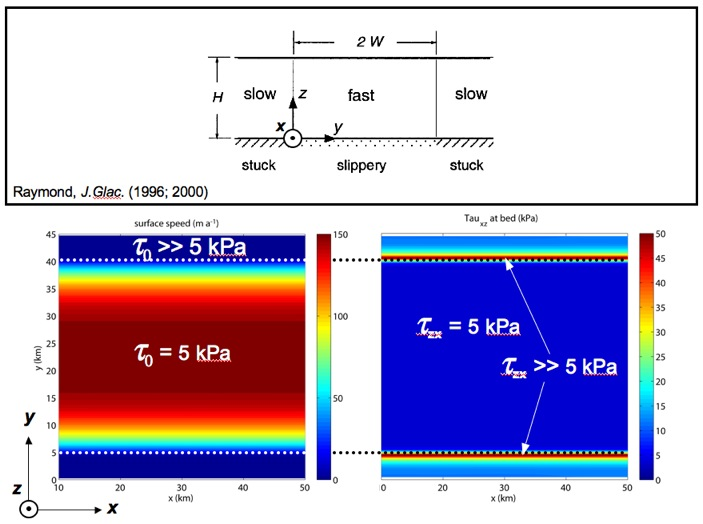
\includegraphics[width=0.9\columnwidth]{\dir/figs/Plastic_bed1.jpg}
%  \end{center}
%  \caption{Idealized ice stream with plastic-bed sliding. Top panel shows a schematic of an idealized ice stream, frozen at the margins and thawed within the ice stream (flow is out of the page). Bottom panel (color) shows a modeled, idealized ice stream (flow is from left to right) with a yield stress of 5 kPa within the ice stream and much larger than 5 kPa outside of it. Bottom left shows the ice stream speed and the bottom right shows the basal drag. Within the ice stream basal drag is equal to the yield stress. Outside of the ice stream, stress transfer to the lateral margins results in basal drag that is much larger than the yield stress (and much larger than the driving stress).}
%  \label{fig:plasticbed1}
%\end{figure} 

%\begin{figure}
%  \begin{center}
%    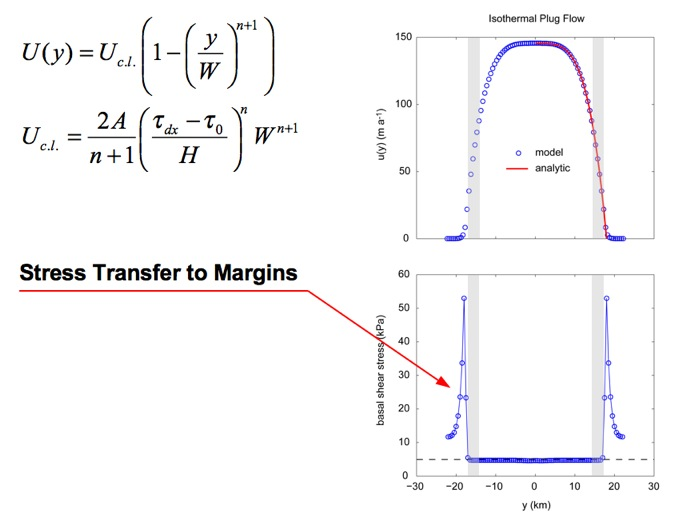
\includegraphics[width=0.9\columnwidth]{\dir/figs/Plastic_bed2.jpg}
%  \end{center}
%  \caption{Across-flow profiles of velocity and basal drag from the modeled, idealized ice stream in Figure 1. In the top panel, the analytical solution from \textit{Raymond} (2005) is also shown for comparison. In the bottom panel, stress transfer to the lateral margins is clearly seen.}
%    \label{fig:plasticbed2}
%\end{figure} 

\subsection{Lateral Boundary Conditions}
Currently, the only lateral boundary condition implemented that is of any significance is that for floating ice; the depth-averaged stress resulting from an adjacent column of ocean water is applied at the location of an ice shelf (or ice tongue) front. The derivation follows largely along the lines above for the free surface and specified basal traction boundary conditions, except that the surface normal vectors, $n_{x}$ and $n_{y}$, are taken as lying entirely in the $x$, $y$ plane (that is, they are perpendicular to a vertical shelf front). Thus we have

\begin{align*}
  & \hat{x}:\quad 4\eta \frac{\partial u}{\partial x}n_{x}+\eta \frac{\partial u}{\partial y}n_{y}+\eta \frac{\partial u}{\partial z}n_{z}=-2\eta \frac{\partial v}{\partial y}n_{x}-\eta \frac{\partial v}{\partial x}n_{y}+\rho g\left( s-z \right)n_{x}-S_{x}, \\ 
 & \hat{y}:\quad 4\eta \frac{\partial v}{\partial y}n_{y}+\eta \frac{\partial v}{\partial x}n_{x}+\eta \frac{\partial v}{\partial z}n_{z}=-2\eta \frac{\partial u}{\partial x}n_{y}-\eta \frac{\partial u}{\partial y}n_{x}+\rho g\left( s-z \right)n_{y}-S_{y} \\ 
\end{align*}

where $S_x$ and $S_y$ are source terms from the pressure due to ocean water (to be defined below) and $\rho g\left( s-z \right)$ comes from including the 1st order vertical stress balance,

\begin{align*}
  & \frac{\partial \sigma _{zz}}{\partial z}=\frac{\partial \tau _{zz}}{\partial z}-\frac{\partial P}{\partial z}=\rho g\quad \text{(integrate w}\text{.r}\text{.t}\text{. z)}, \\ 
 & P=\rho g\left( s-z \right)+\tau _{zz}, \\ 
 & P=\rho g\left( s-z \right)+2\eta \dot{\varepsilon }_{zz}=\rho g\left( s-z \right)+2\eta \left( -\frac{\partial u}{\partial x}-\frac{\partial v}{\partial y} \right), \\ 
\end{align*}

with \textit{\(\rho{}\)} being the ice density. In the last step above we have used the constitutive relation and incompressibility to expand the vertical, normal-deviatoric stress in terms of the effective viscosity and horizontal-normal strain rates. We calculate the source terms $S_x$ and $S_y$ as the depth-averaged stress at the ice shelf front due to the pressure of ocean water there. This value is given by

\begin{align*}
S_{i}=\left[ \frac{1}{H}\frac{1}{2}\rho _{w}g\left( H-h \right)^{2} \right]n_{i}=\left[ \frac{1}{2}\rho _{w}gH\left( \frac{\rho }{\rho _{w}} \right)^{2} \right]n_{i},\quad \quad h=H\left( 1-\frac{\rho _{{}}}{\rho _{w}} \right),
\end{align*}

where  \textit{i=x,y}, $n_i$ is the shelf-front normal vector, $H$ is the ice thickness, $h$ is the ``freeboard'', or ice thickness above floatation, and $\rho_w$ is the density of ocean water. Because we have taken a depth-average for this source term, we take a depth-average of the term $\rho g\left( s-z \right)$ above, which is $\frac{1}{2}\rho gH$.

Combining these two terms and inserting them in the horizontal boundary condition expressions above gives

\begin{align*}
& \hat{x}:\quad 4\eta \frac{\partial u}{\partial x}n_{x}+\eta \frac{\partial u}{\partial y}n_{y}+\eta \frac{\partial u}{\partial z}n_{z}= \\
& -2\eta \frac{\partial v}{\partial y}n_{x}-\eta \frac{\partial v}{\partial x}n_{y}+\left[ -\frac{1}{2}H\left( \frac{\rho }{\rho _{w}} \right)^{2}\rho _{w}g+\frac{1}{2}\rho gH \right]n_{x}, \\ 
 & \hat{y}:\quad 4\eta \frac{\partial v}{\partial y}n_{y}+\eta \frac{\partial v}{\partial x}n_{x}+\eta \frac{\partial v}{\partial z}n_{z}= \\
 & -2\eta \frac{\partial u}{\partial x}n_{y}-\eta \frac{\partial u}{\partial y}n_{x}+\left[ -\frac{1}{2}H\left( \frac{\rho }{\rho _{w}} \right)^{2}\rho _{w}g+\frac{1}{2}\rho gH \right]n_{y}, \\ 
\end{align*}

which can be rearranged to

\begin{align*}
  & \hat{x}:\quad 4\frac{\partial u}{\partial x}n_{x}+\frac{\partial u}{\partial y}n_{y}+\frac{\partial u}{\partial z}n_{z}=-2\frac{\partial v}{\partial y}n_{x}-\frac{\partial v}{\partial x}n_{y}+\frac{\rho gH}{2\eta }\left( 1-\frac{\rho }{\rho _{w}} \right)n_{x}, \\ 
 & \hat{y}:\quad 4\frac{\partial v}{\partial y}n_{y}+\frac{\partial v}{\partial x}n_{x}+\frac{\partial v}{\partial z}n_{z}=-2\frac{\partial u}{\partial x}n_{y}-\frac{\partial u}{\partial y}n_{x}+\frac{\rho gH}{2\eta }\left( 1-\frac{\rho }{\rho _{w}} \right)n_{y}. \\ 
\end{align*}

For an ice shelf, the surface and basal velocities are equal, in which case the vertical velocity gradient terms are $\sim{0}$, giving the final form of the lateral boundary conditions implemented in the model,

\begin{align*}
  & \hat{x}:\quad 4\frac{\partial u}{\partial x}n_{x}+\frac{\partial u}{\partial y}n_{y}=-2\frac{\partial v}{\partial y}n_{x}-\frac{\partial v}{\partial x}n_{y}+\frac{\rho gH}{2\eta }\left( 1-\frac{\rho }{\rho _{w}} \right)n_{x}, \\ 
 & \hat{y}:\quad 4\frac{\partial v}{\partial y}n_{y}+\frac{\partial v}{\partial x}n_{x}=-2\frac{\partial u}{\partial x}n_{y}-\frac{\partial u}{\partial y}n_{x}+\frac{\rho gH}{2\eta }\left( 1-\frac{\rho }{\rho _{w}} \right)n_{y}. \\ 
\end{align*}

\subsection{Summary}
Note that the form for ALL of the boundary conditions above is very similar. In fact, all that differs among the equations for the free surface, the specified basal traction, and the lateral shelf boundary condition is (1) the definition of the normal vectors and (2) the existence and definition of a source term. Here are the \textit{x} direction equations again for the three cases:

\begin{align*}
  & \hat{x}:\quad 4\frac{\partial u}{\partial x}\frac{\partial s}{\partial x}+ \frac{\partial u}{\partial y}\frac{\partial s}{\partial y}-\frac{\partial u}{\partial z}=-2 \frac{\partial v}{\partial y}\frac{\partial s}{\partial x}-\frac{\partial v}{\partial x}\frac{\partial s}{\partial y}, \\ 
  & \hat{x}:\quad 4\frac{\partial u}{\partial x}\frac{\partial b}{\partial x}+\frac{\partial u}{\partial y}\frac{\partial b}{\partial y}-\frac{\partial u}{\partial z}=-2\frac{\partial v}{\partial y}\frac{\partial b}{\partial x}-\frac{\partial v}{\partial x}\frac{\partial b}{\partial y}-\frac{\tau _{bx}}{\eta }, \\ 
  & \hat{x}:\quad 4\frac{\partial u}{\partial x}n_{x}+\frac{\partial u}{\partial y}n_{y}=-2\frac{\partial v}{\partial y}n_{x}-\frac{\partial v}{\partial x}n_{y}+\frac{\rho gH}{2\eta }\left( 1-\frac{\rho }{\rho _{w}} \right)n_{x}. \\
\end{align*}

In the first equation (free surface), the normals are related to the ice sheet surface slope and the source term is zero (which subsequently allows us to divide through by the effective viscosity and remove it from the equations). In the second equation (specified basal traction), the normals are related to the bedrock slopes and the source term is related to the assumed relationship between the basal shear stress and the basal sliding rate. In the last equation, the normals are defined by the shape of the ice-shelf front in map view, the vertical velocity gradient terms are absent, and the source term is related to the pressure from the adjacent column of ocean water.

%\end{document}

\section{Numerical Solution of Higher-Order Equations}

\textbf{SP: Note that I've re-written some of this to be more generic, so that it might still be useful placeholder material in the short term.}

\subsection{Governing Equations}
The final form of the equations we'd like to solve is:
 
%\begin{align*}
% & x: \quad 4\frac{\partial }{\partial x}\left( \eta \frac{\partial u}{\partial x} \right)+\frac{\partial }{\partial y}\left( \eta \frac{\partial u}{\partial y} \right)+\frac{\partial }{\partial z}\left( \eta \frac{\partial u}{\partial z} \right) + \\
% & 2\frac{\partial }{\partial x}\left( \eta \frac{\partial v}{\partial y} \right)+\frac{\partial }{\partial y}\left( \eta \frac{\partial v}{\partial x} \right) = \rho g\frac{\partial s}{\partial x} \\ 
% & y: \quad 4\frac{\partial }{\partial y}\left( \eta \frac{\partial v}{\partial y} \right)+\frac{\partial }{\partial x}\left( \eta \frac{\partial v}{\partial x} \right)+\frac{\partial }{\partial z}\left( \eta \frac{\partial v}{\partial z} \right) + \\
% & 2\frac{\partial }{\partial y}\left( \eta \frac{\partial u}{\partial x} \right)+\frac{\partial }{\partial x}\left( \eta \frac{\partial u}{\partial y} \right) = \rho g\frac{\partial s}{\partial y} \\ 
%\end{align*}

\begin{align*}
 & x: \quad 4\frac{\partial }{\partial x}\left( \eta \frac{\partial u}{\partial x} \right)+\frac{\partial }{\partial y}\left( \eta \frac{\partial u}{\partial y} \right)+\frac{\partial }{\partial z}\left( \eta \frac{\partial u}{\partial z} \right) + 2\frac{\partial }{\partial x}\left( \eta \frac{\partial v}{\partial y} \right)+\frac{\partial }{\partial y}\left( \eta \frac{\partial v}{\partial x} \right) = \rho g\frac{\partial s}{\partial x} \\ 
 & y: \quad 4\frac{\partial }{\partial y}\left( \eta \frac{\partial v}{\partial y} \right)+\frac{\partial }{\partial x}\left( \eta \frac{\partial v}{\partial x} \right)+\frac{\partial }{\partial z}\left( \eta \frac{\partial v}{\partial z} \right) + 2\frac{\partial }{\partial y}\left( \eta \frac{\partial u}{\partial x} \right)+\frac{\partial }{\partial x}\left( \eta \frac{\partial u}{\partial y} \right) = \rho g\frac{\partial s}{\partial y} \\ 
\end{align*}

%% SP: For Glissade, we don't do this (I don't think), so I'm commenting out this section for now.

%\subsection{Coordinate Transform}
%For ice sheet modeling, it is convenient to recast the governing equations using a dimensionless, stretched vertical coordinate (often called a sigma coordinates). The stretched vertical coordinate is defined as:
%
%\begin{align*}
%\sigma = \frac{(s - z)}{H}.
%\end{align*}
%
%This means that at the surface of the ice sheet $\sigma = 0$, and at the base $\sigma = 1$ regardless of the ice thickness.  As a result of this transformation, a coordinate ($x,y,z$) is mapped to ($x',y',\sigma$).  This means that function derivatives must be re-written (using $\frac{\partial f}{\partial x}$ as an example) as:
%
%\begin{align*}
%\frac{\partial f}{\partial x} = \frac{\partial f}{\partial x'} \frac{\partial x'}{\partial x} + \frac{\partial f}{\partial y'} \frac{\partial y'}{\partial x} + \frac{\partial f}{\partial \sigma} \frac{\partial \sigma}{\partial x}.
%\end{align*}
%
%Similarly for $\frac{\partial f}{\partial y}$ and $\frac{\partial f}{\partial z}$. We can simplify this by assuming that 
%
%\begin{align*}
%\frac{\partial x'}{\partial x}, \frac{\partial y'}{\partial y} = 1
%\end{align*}
%
%and
%
%\begin{align*}
%\frac{\partial x'}{\partial y}, \frac{\partial x'}{\partial z}, \frac{\partial y'}{\partial x}, \frac{\partial y'}{\partial z} = 0,
%\end{align*}
%
%which is valid if the bed and surface gradients are not too large. This simplifies the above to:
%
%\begin{align*}
%\frac{\partial f}{\partial x} = \frac{\partial f}{\partial x'} + \frac{\partial f}{\partial \sigma}\frac{\partial \sigma}{\partial x},
%\end{align*}
%
%\begin{align*}
%\frac{\partial f}{\partial y} = \frac{\partial f}{\partial y'} + \frac{\partial f}{\partial \sigma}\frac{\partial \sigma}{\partial y},
%\end{align*}
%
%\begin{align*}
%\frac{\partial f}{\partial z} = \frac{\partial f}{\partial \sigma}\frac{\partial \sigma}{\partial z}.
%\end{align*}
%
%Rescaling parameters $a_{x}$, $a_{y}$, $b_{x}$, $b_{y}$, and $c_{xy}$ are defined. For the $x$ derivative case (the $y$ derivative case is analogous) we have
%
%\begin{align*}
%a_{x} = \frac{1}{H}(\frac{\partial s}{\partial x'} - \sigma \frac{\partial H}{\partial x'}),
%\end{align*}
%
%\begin{align*}
%b_{x} = \frac{\partial a_x}{\partial x'} + a_x \frac{\partial a_x}{\partial \sigma} 
%    = \frac{1}{H} (\frac{\partial^2 s}{\partial x'^2} - \sigma \frac{\partial^2 H}{\partial x'^2} - 2a_x \frac{\partial H}{\partial x'}),
%\end{align*}
%
%\begin{align*}
%c_{xy} = \frac{\partial a_y}{\partial x'} + a_x \frac{\partial a_y}{\partial \sigma} 
%       = \frac{\partial a_x}{\partial y'} + a_y \frac{\partial a_x}{\partial \sigma}.
%\end{align*}
%
%Using these, expressions for the $x$ derivatives become:
%
%\begin{align*}
%\frac{\partial f}{\partial x} = \frac{\partial f}{\partial x'} + a_x \frac{\partial f}{\partial \sigma},
%\end{align*}
%
%\begin{align*}
% & \frac{\partial }{\partial x}\left( \eta \frac{\partial u}{\partial x} \right)=\frac{\partial }{\partial \hat{x}}\left( \eta \frac{\partial u}{\partial \hat{x}} \right)+\frac{\partial \sigma }{\partial \hat{x}}\frac{\partial }{\partial \sigma }\left( \eta \frac{\partial u}{\partial \hat{x}} \right)+\frac{\partial \sigma }{\partial \hat{x}}\frac{\partial }{\partial \hat{x}}\left( \eta \frac{\partial u}{\partial \sigma } \right)+ \\
%& \left( \frac{\partial \sigma }{\partial \hat{x}} \right)^{2}\frac{\partial }{\partial \sigma }\left( \eta \frac{\partial u}{\partial \sigma } \right)+\left( \frac{\partial _{{}}^{2}\sigma }{\partial \hat{x}_{{}}^{2}} \right)\eta \frac{\partial u}{\partial \sigma }
%\end{align*}
%
%where hatted values refer to the coordinate directions in sigma coordinates. Similarly, the first cross-stress term on the RHS is given by
%
%\begin{align*}
%&\frac{\partial }{\partial x}\left( \eta \frac{\partial v}{\partial y} \right)=\frac{\partial }{\partial \hat{x}}\left( \eta \frac{\partial v}{\partial \hat{y}} \right)\,+\frac{\partial \sigma }{\partial \hat{x}}\frac{\partial }{\partial \sigma }\left( \eta \frac{\partial v}{\partial \hat{y}} \right)\,+\frac{\partial \sigma }{\partial \hat{y}}\frac{\partial }{\partial \hat{x}}\left( \eta \frac{\partial v}{\partial \sigma } \right)\,+ \\
%&\frac{\partial \sigma }{\partial \hat{x}}\frac{\partial \sigma }{\partial \hat{y}}\frac{\partial }{\partial \sigma }\left( \eta \frac{\partial v}{\partial \sigma } \right)\,+\frac{\partial _{{}}^{2}\sigma }{\partial \hat{x}\partial \hat{y}}\eta \frac{\partial v}{\partial \sigma }\,
%\end{align*}
%
%
%One term has become five terms and each one of those is pretty ugly looking on its own. Luckily, there is a lot of symmetry here. Notice that if we wanted to design subroutines to discretize the terms on the RHS, we could re-use a lot of them by either applying them to the correct velocity component (to either the $u$ or the $v$ discretization) or by passing the appropriate arguments (by passing either the grid spacing in the $x$ direction or the $y$ direction, where appropriate).
%
%A similar transform is applied to each of the terms in the governing equations given above. At any point within the grid, the grid spacing, coordinate transform, and viscosity information associated with the unknown velocity components is made discrete using finite differences. This information ultimately equates to coefficients on the unknown velocities, allowing the governing equations over the entire grid (with appropriate discretizations for boundary conditions) to be recast as a system of $n$ equations in $n$ unknowns. In turn, this system is solved using standard linear algebraic methods for large, sparse systems of linear equations.


%% SP: For Glissade, we don't do this either, so commenting out this section for now. Note that I've copied some of it below in a new section, which gives a generic discussion of the matrix
%% form, to lead in to solution methods.

%\subsection{Operating Splitting}
%In the governing equations given above, note that for the \textit{x} equation we have moved all terms containing gradients in \textit{v} to the right-hand side (RHS) (and vice-versa for the \textit{y} equation). 
%
%This allows us to solve the equations using an $operator$ $splitting$ approach; for the $x$ equation, we treat $v$ as known (where we take the values of $v$ from the previous iteration, as discussed further below) and solve for $u$, and vice versa when we solve the $y$ equation for $v$. The splitting refers to the fact that we are breaking the multi-dimensional divergence operation into two steps; rather than solving one big matrix equation for $u$ and $v$ simultaneously, we solve two smaller matrix equations in sequence with one of the unknowns treated as a known source term on the RHS of the equation. This procedure was probably more common and important years ago when it was desirable to keep the matrix equations as small as possible for memory management issues. On today's machines, with fewer memory limitations (in particular when dealing with codes designed to run on parallel, distributed memory architectures) this splitting is not necessary and may even lead to some undesirable numerical side effects (i.e. a slow-down in the convergence of iterations used to treat nonlinearity in the governing equations).
%
%A general matrix form of the split equations, where coefficients on the $u$ and $v$ velocity components (i.e. viscosity, grid spacing, scalars) are contained in the block matrices \textbf{A}, is given by 
%
%\begin{align*}
%\begin{matrix}
%  \left[ \begin{matrix}
%   \mathbf{A}_{\mathbf{uu}} & \mathbf{0}  \\
%   \mathbf{0} & \mathbf{A}_{\mathbf{vv}}  \\
%\end{matrix} \right]\left[ \begin{matrix}
%   \mathbf{u}  \\
%   \mathbf{v}  \\
%\end{matrix} \right]=\left[ \begin{matrix}
%   \mathbf{b}_{\mathbf{u}}-\mathbf{A}_{\mathbf{uv}}\mathbf{v}  \\
%   \mathbf{b}_{\mathbf{v}}-\mathbf{A}_{\mathbf{vu}}\mathbf{u}  \\
%\end{matrix} \right] \\ 
%   \\ 
%  \mathbf{A}_{\mathbf{uu}}\mathbf{u}=\mathbf{b}_{\mathbf{u}}-\mathbf{A}_{\mathbf{uv}}\mathbf{v},\quad \quad \mathbf{A}_{\mathbf{vv}}\mathbf{v}=\mathbf{b}_{\mathbf{v}}-\mathbf{A}_{\mathbf{vu}}\mathbf{u} \\ 
%\end{matrix}
%\end{align*}
%
%where the \textbf{uu} subscript denotes block matrices containing coefficients for gradients on \textit{u} in the equation for the \textit{x} component of velocity (i.e. \textit{u}). The subscript \textbf{uv} denotes block matrices containing coefficients for gradients on \textit{v} in the equation for the \textit{x} component of velocity (and similarly for the \textbf{vv} and \textbf{vu} subscripts). On the right-hand side, the single subscripts \textbf{u} and \textbf{v} are attached to the geometric source terms for the \textit{x} and \textit{y} components of velocity, respectively.

Any number of standard methods (e.g., Finite Differences, Finite Volumes, or Finite Elements) can be used to ``discretize" the above governing equations. That is, to re-formulate them from their continuous, PDE form, into a discontinuous, piecewise, algebraic approximation based on a specific computational mesh. In the limit, as the mesh spacing goes to zero, the difference between the solution to the actual PDE and its algebraic approximation also goes to zero. The GLISSADE dynamical core uses the Finite Element Method (FEM) to discretize the governing equations, which is discussed in more detail in \textbf{pointer to Bill's chapter on the discretization here}. In general, the result of the discretization is a set of linear, algebraic equations that can be written in a matrix form. An example is given below, where where the coefficients on the $u$ and $v$ velocity components (i.e. viscosity, grid spacing, scalars) are contained in the block matrices \textbf{A}, given by 

\begin{align*}
\begin{matrix}
  \left[ \begin{matrix}
   \mathbf{A}_{\mathbf{uu}} & \mathbf{A}_{\mathbf{uv}}  \\
   \mathbf{A}_{\mathbf{vu}} & \mathbf{A}_{\mathbf{vv}}  \\
\end{matrix} \right]\left[ \begin{matrix}
   \mathbf{u}  \\
   \mathbf{v}  \\
\end{matrix} \right]=\left[ \begin{matrix}
   \mathbf{b}_{\mathbf{u}}  \\
   \mathbf{b}_{\mathbf{v}}  \\
\end{matrix} \right] \\ 
   \\ 
  \mathbf{A}_{\mathbf{uu}}\mathbf{u} + \mathbf{A}_{\mathbf{uv}}\mathbf{v} =\mathbf{b}_{\mathbf{u}},
  \quad \quad \mathbf{A}_{\mathbf{vu}}\mathbf{u} + \mathbf{A}_{\mathbf{vv}}\mathbf{v} =\mathbf{b}_{\mathbf{v}} \\ 
\end{matrix}
\end{align*}

where the \textbf{uu} subscript denotes block matrices containing coefficients for gradients on \textit{u} in the equation for the \textit{x} component of velocity (i.e. \textit{u}). The subscript \textbf{uv} denotes block matrices containing coefficients for gradients on \textit{v} in the equation for the \textit{x} component of velocity (and similarly for the \textbf{vv} and \textbf{vu} subscripts). On the right-hand side, the single subscripts \textbf{u} and \textbf{v} are attached to the geometric source terms for the \textit{x} and \textit{y} components of velocity, respectively.

\subsection{Solution of the Non-linear System Through a Fixed Point Iteration}
The non-linearity in the equations -- the fact that the coefficients on the velocity components (the viscosity) are dependent on the velocity (or more specifically, the velocity gradients) -- is handled through a fixed-point iteration. A general fixed point iteration for a vector of unknowns \textit{u} can be written as 

\begin{align*}
u^{k}=\mathbf{B}\left( u^{k-1} \right),
\end{align*}

where \textit{k} is the index for the \textit{u} being solved for and \textbf{B} is a matrix operation performed on the components of \textit{u} obtained at the previous iteration, \textit{k-1}. The fixed point occurs when the values of \textit{u} at \textit{k} and \textit{k-1} are equal to within some given tolerance (at which point the iteration process is halted). %CISM has options for implementing both Picard and Newton-based fixed-point iterations. 
For a Picard iteration, which is currently standard when using GLISSADE, the matrix coefficients with a velocity dependence are simply based on the velocities obtained at the previous iteration. In most cases, this equates to using velocities obtained from the previous iteration to calculate the strain rate components that go into the calculation of the effective viscosity, $\eta$.

\section{Final Matrix Form}
When accounting for %both the operator splitting and 
the Picard iteration on the effective viscosity, the final form of the matrix equations solved by GLISSADE becomes 

%% SP: This is the split form - below is the more general (non-split) version
%\begin{align*}
%\begin{matrix}
%  \left[ \begin{matrix}
%   \mathbf{A}_{\mathbf{uu}}^{k-1} & \mathbf{0}  \\
%   \mathbf{0} & \mathbf{A}_{\mathbf{vv}}^{k-1}  \\
%\end{matrix} \right]\left[ \begin{matrix}
%   \mathbf{u}^{k}  \\
%   \mathbf{v}^{k}  \\
%\end{matrix} \right]=\left[ \begin{matrix}
%   \mathbf{b}_{\mathbf{u}}-\mathbf{A}_{\mathbf{uv}}^{k-1}\mathbf{v}^{k-1}  \\
%   \mathbf{b}_{\mathbf{v}}-\mathbf{A}_{\mathbf{vu}}^{k-1}\mathbf{u}^{k-1}  \\
%\end{matrix} \right] \\ 
%   \\ 
%  \mathbf{A}_{\mathbf{uu}}^{k-1}\mathbf{u}=\mathbf{b}_{\mathbf{u}}-\mathbf{A}_{\mathbf{uv}}^{k-1}\mathbf{v}^{k-1},\quad \quad \mathbf{A}_{\mathbf{vv}}^{k-1}\mathbf{v}=\mathbf{b}_{\mathbf{v}}-\mathbf{A}_{\mathbf{vu}}^{k-1}\mathbf{u}^{k-1} \\ 
%\end{matrix}
%\end{align*}

\begin{align*}
\begin{matrix}
  \left[ \begin{matrix}
   \mathbf{A}_{\mathbf{uu}}^{k-1} & \mathbf{A}_{\mathbf{uv}}^{k-1}  \\
   \mathbf{A}_{\mathbf{vu}}^{k-1} & \mathbf{A}_{\mathbf{vv}}^{k-1}  \\
\end{matrix} \right]\left[ \begin{matrix}
   \mathbf{u}^{k}  \\
   \mathbf{v}^{k}  \\
\end{matrix} \right]=\left[ \begin{matrix}
   \mathbf{b}_{\mathbf{u}}^{k}  \\
   \mathbf{b}_{\mathbf{v}}^{k}  \\
\end{matrix} \right] \\ 
   \\ 
  \mathbf{A}_{\mathbf{uu}}^{k-1}\mathbf{u}^{k} + \mathbf{A}_{\mathbf{uv}}^{k-1}\mathbf{v}^{k} =\mathbf{b}_{\mathbf{u}}^{k},
  \quad \quad \mathbf{A}_{\mathbf{vu}}^{k-1}\mathbf{u}^{k} + \mathbf{A}_{\mathbf{vv}}^{k-1}\mathbf{v}^{k} =\mathbf{b}_{\mathbf{v}}^{k} \\ 
\end{matrix}
\end{align*}

where the index \textit{k} denotes value associated with the current non-linear iteration (in the case of velocities, these are the values being solved for and in the case of the geometric forcing terms, these are the values associated with the current time step) and the index \textit{k}-1 denotes a lagged value taken from solution at the end of the previous non-linear iteration (again, here the lagging is primarily with respect to the effective viscosity, the value of which is calculated using velocity gradients obtained at the end of the previous iteration). The final form of the matrix equations given above represents a linear system; for the solution at any particular nonlinear iteration \textit{k}, all of the coefficients on the unknown velocity components \textit{u} and \textit{v} are held frozen during the solution of the linear system. This linear system can be solved using any practical method. For large, sparse systems, the preconditioned conjugate gradient (PCG) method, or some related variant (e.g., preconditioned BiCG or GMRES) is generally the most efficient. In this case the linear system is not solved exactly but is solved to within some small tolerance of the true solution.

%% SP: commenting this out for now, since Newton is not currently an option (but leaving in as a possibility for use in later versions)

%\subsection{Newton-based Methods for Solutions of the Non-linear System}
%Without any operator splitting, the generic matrix form of the equations to be solved can be written as
%
%\begin{align*}
%\mathbf{A}(\mathbf{u})\mathbf{u}=\mathbf{b}.
%\end{align*}
%
%The linearized form of the equations to be solved using the Picard solution can be written as
%
%\begin{align*}
%\mathbf{u}^{k}=\mathbf{A}(\mathbf{u}^{k-1})^{-1}\mathbf{b}.
%\end{align*}
%
%The full nonlinear system to be solved can be written as
%
%\begin{align*}
%\mathbf{F}(\mathbf{u})=\mathbf{A}(\mathbf{u})\mathbf{u}-\mathbf{b}
%\end{align*}
%
%with the solution for the uknown vector \textit{u} given by 
%
%\begin{align*}
%\mathbf{F}(\mathbf{u})=0.
%\end{align*}
%
%A Newton-based solution for this system of equations, based on a first-order Taylor series expansion about the solution for \textit{u} at iteration \textit{k-1}, can be written as
%
%\begin{align*}
%\mathbf{F}(\mathbf{u}^{k})=\mathbf{F}(\mathbf{u}^{k-1})+\mathbf{F}(\mathbf{u}^{k-1})\delta \mathbf{u}^{k-1},
%\end{align*}
%
%where
%
%\begin{align*}
%\mathbf{F}(\mathbf{u}^{k-1})=\mathbf{J}^{k-1}
%\end{align*}
%
%is the system Jacobian with individual components give by
%
%\begin{align*}
%J_{ij}=\frac{\partial F_{i}(\mathbf{u}^{k-1})}{\partial u_{j}}
%\end{align*}
%
%and 
%
%\begin{align*}
%\delta \mathbf{u}^{k-1}=\mathbf{u}^{k}-\mathbf{u}^{k-1}
%\end{align*}
%
%is the Newton update to be solved for. One method for doing so is by solving 
%
%\begin{align*}
%\delta \mathbf{u}^{k-1}=-\left( \mathbf{J}^{k-1} \right)^{-1}\mathbf{F}(\mathbf{u}^{k-1}).
%\end{align*}
%
%The advantage of Newton-based methods is that, with a good initial guess for the solution, convergence rates are very often quadratic (e.g. the residual decreases quadratically, so that at iteration \textit{k} one has a residual of 0.1, at iteration \textit{k+1}, a residual of 0.01, and at iteration \textit{k+2} a residual of 0.0001), whereas Picard-based iterations are much slower to converge. A figure comparing rates of convergence for Picard versus Newton on a CISM tests case is shown below (Figure \ref{fig:jfnk}. The Newton method is based on the work of Lemieux et al. ($J.$ $Comput.$ $Phys.$, \textbf{230}, 2011), which is discussed further below.
%
%\begin{figure}
%  \begin{center}
%    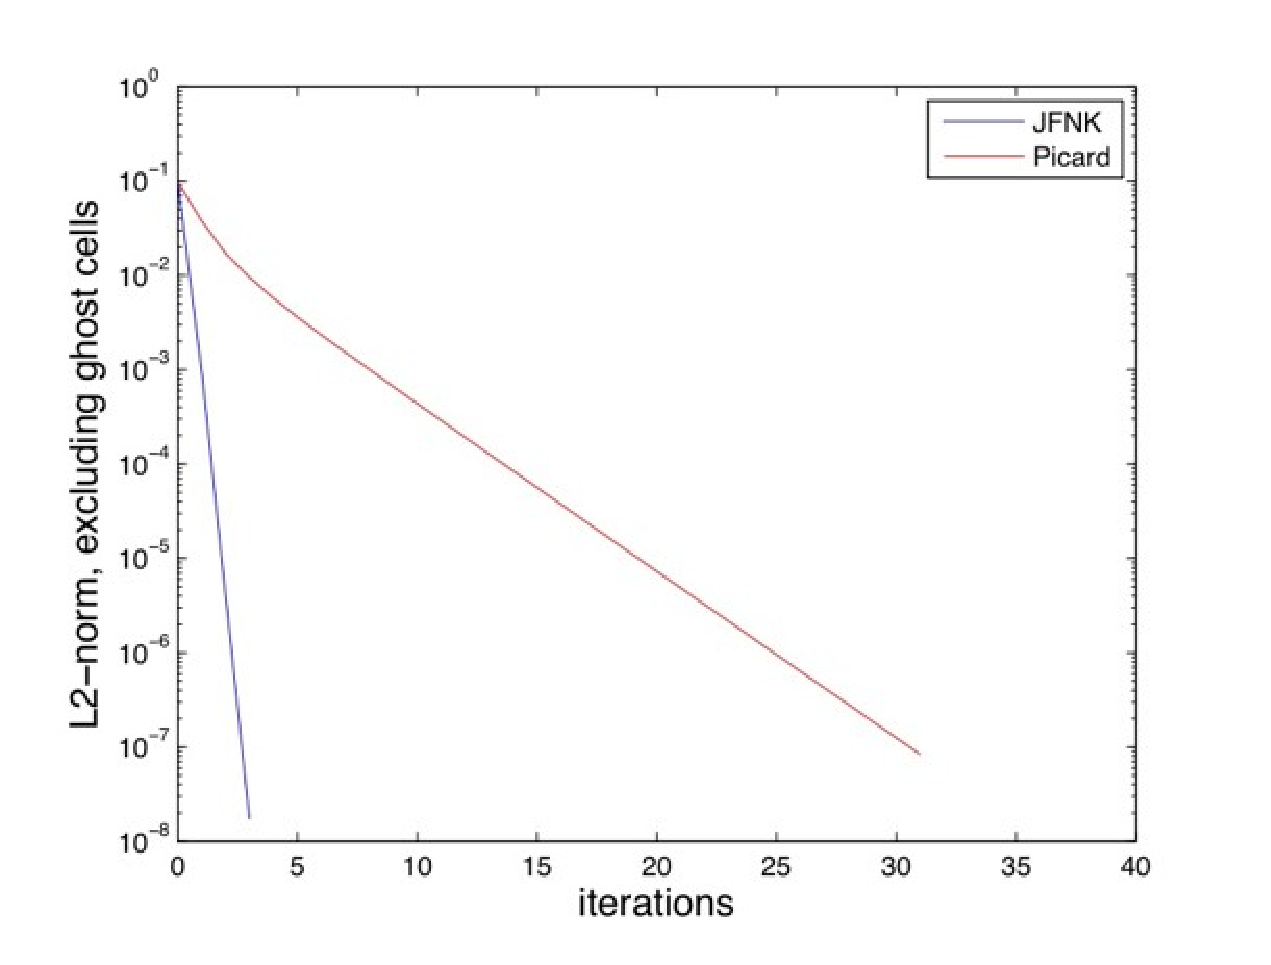
\includegraphics[width=0.9\columnwidth]{\dir/figs/Picard_vs_newton.eps}
%  \end{center}
%  \caption{Rates of convergence for the nonlinear iteration in CISM.}
%  \label{fig:jfnk}
%\end{figure} 
%
%\subsection{The Jacobian Free Approach}
%In practice, the model Jacobian may either be too difficult or to expensive too form. A Jacobian Free Newton-Krylov (JFNK) approach has recently been implemented in CISM (Leimieux et al., 2011), largely following methods discussed in Knoll and Keyes ($J.$ $Comput.$ $Phys.$, \textbf{193}, 2004).
%
%The crux of the method comes from noting that, when solving the last equation above using a Krylov method (e.g. Conjugate Gradients, GMRES, etc.) the solution for the Newton update is taken from a combination of Krylov vectors that span the subspace
%
%
%\begin{align*}
%span\left\{ \mathbf{r}_{0},\mathbf{Jr}_{0},\mathbf{J}^{2}\mathbf{r}_{0},...,\mathbf{J}^{n-1}\mathbf{r}_{0} \right\}=span\left\{ \mathbf{r}_{0},\mathbf{Jv}_{1},\mathbf{Jv}_{2},...,\mathbf{Jv}_{n-1} \right\}.
%\end{align*}
%
%This implies that, when using a Krylov method, one only ever needs to calculate matrix vector products of the form $\mathbf{Jv}$ when building up the subspace that approximates the solution vector $\delta \mathbf{u}$.
%
%Following Knoll and Keyes (2004), note that the necessary matrix vector products can be approximated through nonlinear function evaluations and a perturbation as
%
%\begin{align*}
%\mathbf{Jv}\approx \frac{\mathbf{F}\left( \mathbf{u}+\varepsilon \mathbf{v} \right)-\mathbf{F}\left( \mathbf{u} \right)}{\varepsilon }.
%\end{align*}
%
%It is not immediately obvious why this approximation is valid. To verify this, take a few steps back and consider a nonlinear system of equations of two variables, $u_{1}$ and $u_{2}$. The right-hand side of the above equation can be expanded as
%
%\begin{align*}
%\frac{\mathbf{F}\left( \mathbf{u}+\varepsilon \mathbf{v} \right)-\mathbf{F}\left( \mathbf{u} \right)}{\varepsilon }=\left[ \begin{matrix}
%   \frac{F_{1}\left( u_{1}+\varepsilon v_{1},u_{2}+\varepsilon v_{2} \right)-F_{1}(u_{1},u_{2})}{\varepsilon }  \\
%   \frac{F_{2}\left( u_{1}+\varepsilon v_{1},u_{2}+\varepsilon v_{2} \right)-F_{2}(u_{1},u_{2})}{\varepsilon }  \\
%\end{matrix} \right].
%\end{align*}
%
%A first-order Taylor series expansion approximation to this is given by
%
%\begin{align*}
%\frac{\mathbf{F}\left( \mathbf{u}+\varepsilon \mathbf{v} \right)-\mathbf{F}\left( \mathbf{u} \right)}{\varepsilon }\approx \left[ \begin{matrix}
%   \frac{F_{1}\left( u_{1},u_{2} \right)+\varepsilon v_{1}\frac{\partial F_{1}}{\partial u_{1}}+\varepsilon v_{2}\frac{\partial F_{1}}{\partial u_{2}}-F_{1}(u_{1},u_{2})}{\varepsilon }  \\
%   \frac{F_{2}\left( u_{1},u_{2} \right)+\varepsilon v_{1}\frac{\partial F_{2}}{\partial u_{1}}+\varepsilon v_{2}\frac{\partial F_{2}}{\partial u_{2}}-F_{2}(u_{1},u_{2})}{\varepsilon }  \\
%\end{matrix} \right],
%\end{align*}
%
%which collapses to
%
%\begin{align*}
%\frac{\mathbf{F}\left( \mathbf{u}+\varepsilon \mathbf{v} \right)-\mathbf{F}\left( \mathbf{u} \right)}{\varepsilon }\approx\left[ \begin{matrix}
%   v_{1}\frac{\partial F_{1}}{\partial u_{1}}+v_{2}\frac{\partial F_{1}}{\partial u_{2}}  \\
%   v_{1}\frac{\partial F_{2}}{\partial u_{1}}+v_{2}\frac{\partial F_{2}}{\partial u_{2}}  \\
%\end{matrix} \right].
%\end{align*}
%
%Finally, note that the right-hand side of the above equation is equal to 
%
%\begin{align*}
%\mathbf{Jv}\approx\left[ \begin{matrix}
%   v_{1}\frac{\partial F_{1}}{\partial u_{1}}+v_{2}\frac{\partial F_{1}}{\partial u_{2}}  \\
%   v_{1}\frac{\partial F_{2}}{\partial u_{1}}+v_{2}\frac{\partial F_{2}}{\partial u_{2}}  \\
%\end{matrix} \right],
%\end{align*}
%
%with the Jacobian matrix given by
%
%\begin{align*}
%\mathbf{J}=\left[ \begin{matrix}
%   \frac{\partial F_{1}}{\partial u_{1}} & \frac{\partial F_{1}}{\partial u_{2}}  \\
%   \frac{\partial F_{2}}{\partial u_{1}} & \frac{\partial F_{2}}{\partial u_{2}}  \\
%\end{matrix} \right].
%\end{align*}
%
%The matrix vector product \textbf{Jv} is what needs to be calculated repeatedly while building up the Krylov subspace vectors that combine to approximate the Newton update vector $\delta \mathbf{u}$.
%
%The important point is that at no point in this process does one need to calculate the entire Jacobian matrix. Another important point is that the accuracy of the approximation to the Jacobian is proportional to the small perturbation term, $\varepsilon$.

%\section{References}
%\begin{itemize}
%\item  {Knoll, D.A. and D.E. Keyes. Jacobian-free Newton-Krylov methods: a survey of approaches and applications, \textbf{193}, 357-397, 2004}.
%\end{itemize}
%
%\begin{itemize}
%\item  {Lemieux, J.F., S.F. Price, K.J. Evans, D. Knoll, A.G. Salinger, D. Holland, and A.J. Payne. Implementation of the Jacobian-Free Newton-Krylov method for solving the first-order ice sheet momentum balance, \textit{J. Comput. Phys.}, \textbf{230}, 6531-6545, doi:10.1016/j.jcp.2011.04.037, 2011}.
%\end{itemize}
%
%\end{document}

\section{Thickness Evolution in Higher-Order Models}
\label{sc:ho-thickness-evol}

\subsection{Conservation of mass}
As mentioned previously, conservation of mass for an ice sheet can be expressed by

\begin{align*}
\frac{\partial H}{\partial t}=-\nabla \cdot \left( \vec{U}H \right)+\dot{b},
\end{align*}

where $\vec{U}=(U,V)$ is the 2-dimensional, depth-integrated velocity vector, $H$ is the ice thickness, $\vec{U}H$ is the 2-dimensional ice flux vector, and $\dot{b}$ represents the sum of surface and basal mass balance terms. The change in thickness per unit time is given by the negative of the flux divergence plus a source term. 
%We can expand this a bit as,
%
%\begin{align*}\frac{\partial H}{\partial t}=-\left( \frac{\partial \left( UH \right)}{\partial x}+\frac{\partial \left( VH \right)}{\partial y} \right)+\dot{b}, \\ 
%\end{align*}
%
%where $\vec{U}$ is the depth-averaged velocity vector (in map plane), and \textit{U} and \textit{V} are the depth integrated \textit{x} and \textit{y} velocity fields, \textit{H} is the ice thickness, and $\dot{b}$ is the source term, which is the surface mass balance (>0 for accumulation and <0 for ablation). 
Note that the negative sign in front of the divergence (terms in parentheses on the right-hand side) insures sensible behavior: consider a section of the ice sheet where the thickness is nearly constant and there is no accumulation or ablation. If the velocity gradient along-flow is negative (the ice is slowing down), then we expect local thickening (left-hand side of the equation is $>0$) and vice versa (if the ice is speeding up along flow, we expect local thinning). This is the equation that needs to be solved to calculate the evolution of the ice sheet geometry.

\subsection{A diffusive approach}
For the case of a shallow-ice model, the values of $U$ and $V$ are recast in terms of ice thickness and elevation gradients, in which case the whole problem can be recast as a diffusion equation in ice thickness. In 1-dimension, the equation becomes

\begin{align*}
\frac{\partial H}{\partial t}=\frac{\partial }{\partial x}\left( D\frac{\partial h}{\partial x} \right)+\dot{b},\quad D=\frac{2A}{n+2}\left( \rho g \right)^{n}H^{n+2}\left| \frac{\partial h}{\partial x} \right|^{n-1},
\end{align*}

where $D$ is the non-linear diffusivity (because it depends on the solution to the equation, $H$), $A$ is the rate factor in Glen's flow law, $n$ is the power-law exponent, $h$ is the ice surface elevation, and $\rho$ and $g$ are the ice density and the acceleration due to gravity. Importantly, we need only local information in order to solve the above equation. If our velocity solution can not be solved locally, as in the case of higher-order models, we cannot easily use the above formulation to solve ice sheet evolution. In an attempt to use this form and retain a diffusion-solution approach to the problem (diffusion problems generally have nice numerical properties), we could try the following approach (again, in 1-dimensions only),

\begin{align*}
\frac{\partial H}{\partial t}=\frac{\partial }{\partial x}\left( D\frac{\partial h}{\partial x} \right)+\dot{b},\quad D=UH\left( \frac{\partial h}{\partial x} \right)^{-1},
\end{align*}

where the $U$ in the expression for $D$ is the depth-integrated velocity field from the higher-order model. This is the approach initially taken by \citet{Pattyn:2003tj} in one of the first higher-order modeling studies to deal with this particular problem. Notice that ice sheet surface slope is in the denominator of the diffusivity here and, as slopes get smaller and smaller (as they tend to do in regions of fast flow like ice streams and ice shelves) the diffusivity will get larger and larger (approaching infinity as the slope goes to zero). The faster velocities in these regions appear in the numerator of the diffusivity, also making it larger. This is a severe restriction on this approach because, for explicit schemes, the diffusive CFL condition requires that

\begin{align*}
\Delta t<\frac{\left( \Delta x \right)^{2}}{2D},
\end{align*}

where $\Delta t$ is the time step required for numerical stability and $\Delta x$ is the grid spacing. As the diffusivity goes to infinity (i.e., for faster flows and shallower slopes), the stable time step goes to zero. Thus in practice, this approach has proven very difficult to use for calculating ice sheet evolution in most of the dynamically interesting areas of ice sheets that we are interested in. An alternate approach is needed.

\subsection{Advection schemes}
An alternate approach is to solve the evolution equation using an advection scheme. Numerically, advection schemes can be more problematic than diffusion schemes, but in some cases like this one, they are difficult to avoid. The most general advection scheme is a first-order, upwind-advection scheme (as above, ``first-order" here refers to first-order accurate), and we will outline the implementation of such a scheme below.

Most ice sheet models (and fluid dynamics models in general) perform calculations on a ``staggered" grid of the type shown below in Figure \ref{fig:stag_c_grid}, where velocity components live on one grid and scalar components (e.g. temperatures, pressures, thickness, etc.) live on a grid that is staggered by 1/2 grid space in the horizontal dimensions (this is essential for numerical stability reasons that we won't discuss here).

\begin{figure}
  \begin{center}
    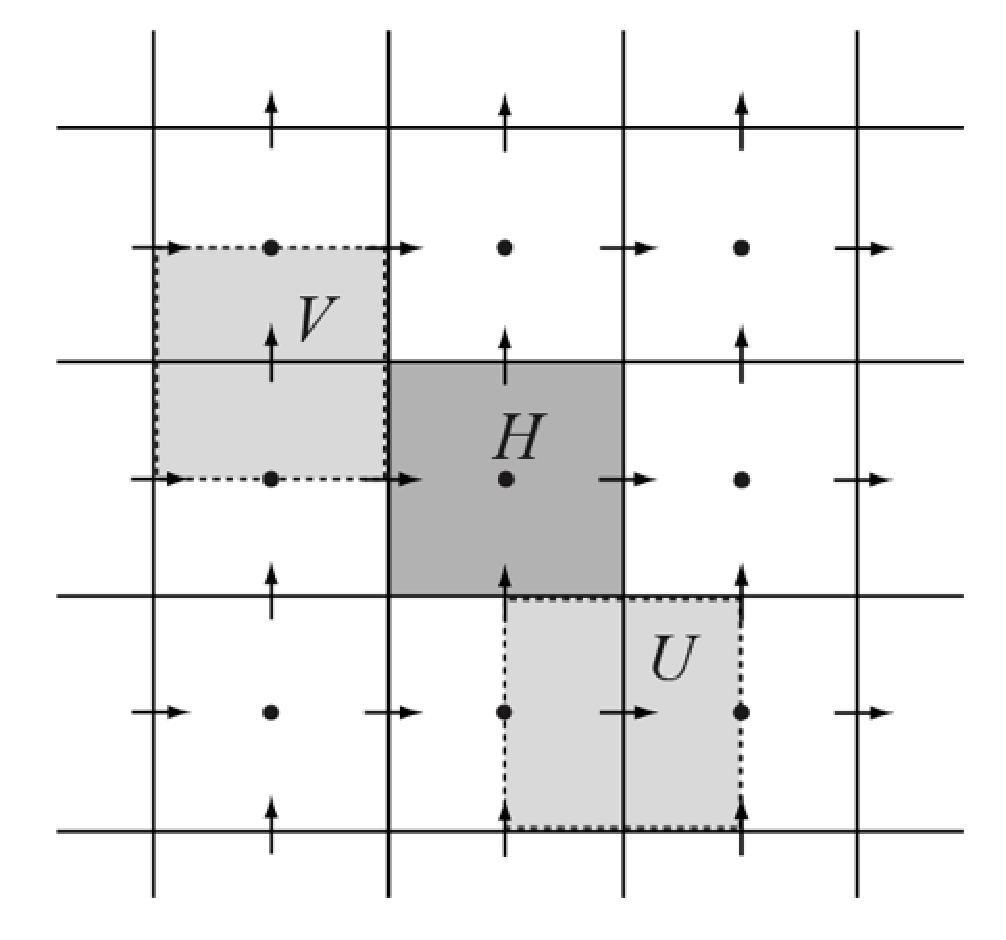
\includegraphics[width=0.4\columnwidth]{\dir/figs/Stag_grid.eps}
  \end{center}
\caption{Staggered grid in two dimensions, showing scalars (like thickness, $H$) at grid cell centers and velocity components, $U$ and $V$, at grid cell faces. This is a ``C" grid. Another staggered-grid possibility is a ``B" grid, for which both velocity components live at the grid cell corners. While CISM uses a B grid, averaging of corner velocities to face centers allows one to express them on a C grid, if necessary.}
  \label{fig:stag_c_grid}
\end{figure} 

A control volume (or finite volume) approach to solving the equation 

\begin{align*}
\frac{\partial H}{\partial t}=-\left( \frac{\partial \left( UH \right)}{\partial x}+\frac{\partial \left( VH \right)}{\partial y} \right)+\dot{b} \\ 
\end{align*}

would be to integrate our equation over a control volume centered on the scalar values (Figures \ref{fig:stag_c_grid} and \ref{fig:stag_c_grid2}). Ignoring source terms for now (assume $\dot{b}=0$), and assuming flow along the \textit{x} direction only (assume $V=0$) we have

\begin{align*}
\frac{\partial H}{\partial t}=-\frac{1}{\Delta y\Delta x}\int_{s}^{n}{\int_{w}^{e}{\frac{\partial \left( UH \right)}{\partial x}}}dxdy=-\frac{1}{\Delta y\Delta x}\left( HU_{e}-HU_{w} \right)\Delta y. \\
\end{align*}

The ``east" and ``west" (subscripts $e$ and $w$) faces of the control volume are shown in Figure \ref{fig:stag_c_grid2}.

\begin{figure}
  \begin{center}
    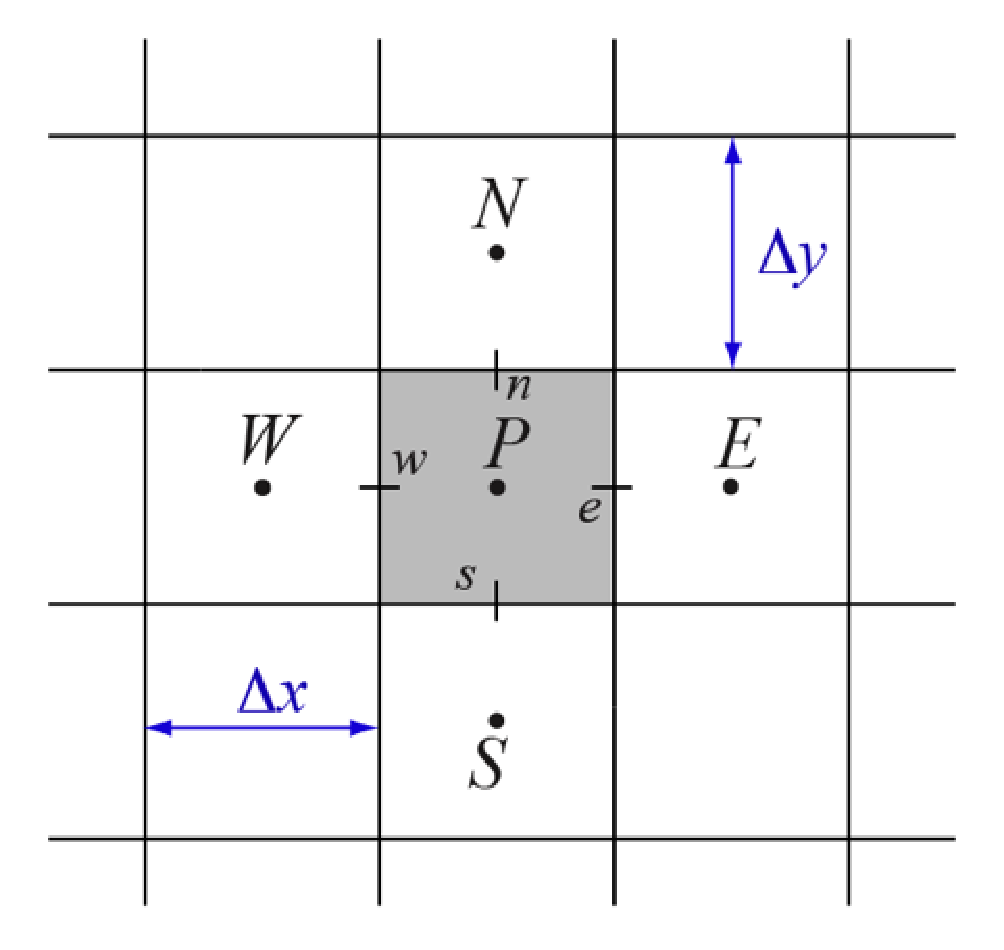
\includegraphics[width=0.4\columnwidth]{\dir/figs/Stag_gridb.eps}
  \end{center}
  \caption{Staggered grid in two dimensions, showing locations of interfaces and control volume dimensions. Interfaces \textit{e}, \textit{w}, \textit{n} and \textit{s} connect the volume centered at \textit{P} with those volumes to the east, west, north, and south (\textit{E}, \textit{W}, \textit{N}, and \textit{S}).}
  \label{fig:stag_c_grid2}
\end{figure} 

In the above equation, we have deliberately left it vague as to which value of $H$ is being advected across the east and west interfaces, into or out of the volume. This is where the term ``upwinding" comes in -- we choose the scalar value to advect across the interface based on an upwinding criterion. If, for example, the flow at interface $e$ is from left to right ($U>0$), we would advect the value of $H$ at $P$ \textit{out} of the volume centered at $P$ and \textit{into} the volume centered at $E$. If, on the other hand, the flow at $e$ was from right to left ($U<0$), we would advect the value of $H$ at $E$ \textit{into} the volume at $P$ and \textit{out} of the volume at $E$. 

The product of velocity, thickness, and the grid spacing at each interface gives a volume flux in units of cubic meters per year. The sum of the volume fluxes over the total number of faces being considered (two in this case, but four for the 2-dimensional case) gives the total volume flux in (total$>$0) or out (total$<$0) of the volume. When this number is divided by the area of the volume, the result is the mean thickness change in that volume, per unit time, that is required to maintain conservation of mass.

\subsection{Explicit vs. Implicit Evolution Schemes}

Is this an explicit or implicit scheme? If we discretize the right-hand side of the primary equation in time we get

\begin{align*}
  & \frac{\partial H}{\partial t}=-\nabla \cdot \left( UH \right)+\dot{b}, \\
 & \frac{H_{t=1}-H_{t=0}}{\Delta t}\approx -\nabla \cdot \left( UH \right)+\dot{b}.\\
\end{align*}

This can be rearranged to,

\begin{align*}
H_{t_{t=1}}\approx H_{t=0}+\left[ -\nabla \cdot \left( UH \right)+\dot{b} \right]_{t=0}\Delta t.
\end{align*}

The thickness at the new time step $t=1$ is a function of \textit{only} variables evaluated at the previous time step $t=0$. Thus, the scheme is \textit{explicit} and, as such, is subject to the advective CFL condition for stability,

\begin{align*}
\Delta t<\frac{\Delta x}{U}.\\
\end{align*}

Essentially, this means that we cannot take such a large time step that we advect mass through more than one volume (past more than one grid space) per time step.

There is not much more to a first-order advection scheme other than extending it to two dimensions for non-zero \textit{V}. The finite volume formulation guarantees that it will be conservative globally (i.e. all mass moved around on the grid is accounted for at each time step). There are many other ``higher-order" advection schemes available (e.g., the incremental remapping scheme used in CISM and described in Chapter \ref{ch:glissade}), but they are mainly based on the principles outlined here and rely on corrections to the simple upwind assumption in order to gain more accuracy.



\chapter{Physics}
\renewcommand{\dir}{physics}

\section{Physics documentation}

\subsection{Ice temperature evolution routines}

\subsubsection{Summary}
Call structure (filenames in brackets).
\begin{itemize}
    \item subroutine testinisthk [glimmer\_setup] and
    \item subroutine glimmer\_i\_tstep [glimmer\_object] call
    \item subroutine timeevoltemp [glimmer\_temp] calls
    \item subroutine calcartm [glimmer\_temp] and
    \item subroutine timeders [glimmer\_thck] and
    \item subroutine gridwvel [glimmer\_velo] and
    \item subroutine wvelintg [glimmer\_velo] and
    \item subroutine chckwvel [glimmer\_velo] and
    \item subroutine finddisp [glimmer\_temp] and
    \item subroutine hadvall [glimmer\_temp] and
    \item subroutine hadvpnt [glimmer\_temp] and
    \item subroutine findvtri [glimmer\_temp] and
    \item subroutine tridag [glimmer\_temp] and
    \item subroutine corrpmpt [glimmer\_temp] and
    \item subroutine swapbndt [glimmer\_temp] and
    \item subroutine calcbmlt [glimmer\_temp] and
    \item subroutine calcflwa [glimmer\_temp]
\end{itemize}

\noindent Modules used.
\begin{itemize}
    \item
\end{itemize}

\subsubsection{Introduction}
The section describes the routines that are concerned with
calculating the three-dimensional distribution of temperature
within the ice mass.  They can be broken down into five groups.
\begin{itemize}
    \item determining air temperature (upper boundary
    condition) [\texttt{calcartm}];
    \item determining vertical velocity field from existing
    horizontal velocity fields (normally only needed if temperature is being calculated) [\texttt{wvelintg}, chckwvel];
    \item routines associated with vertical grid coordinate
    system [\texttt{gridwvel}, \texttt{timeders}];
    \item the main temperature solver [\texttt{finddisp, hadvall, hadvpnt, findvtri, tridag, corrpmpt, swapbndt}];
    \item ancillary calculations that only make sense if temperature is being calculated
    [\texttt{calcbmlt}, \texttt{calcflwa}].
\end{itemize}

The basic quantity returned is a three-dimensional grid of
temperature in $\circ^{-1}$C (uncorrected for variations in
pressure melting point and unscaled).  Temperature is held in the
array \texttt{temp} and will be referred to here using the symbol
$T$.

In addition to temperature a number of other quantities are
calculated by these routines.  They include: basal melt rate ($m$
\texttt{bmlt} m yr$^{-1}$ scaled using \texttt{thk0/tim0}); basal
water depth ($W$ \texttt{bwat} m scaled using \texttt{thk0});
vertical velocity ($w$ \texttt{wvel} m yr$^{-1}$ scaled using
\texttt{thk0/tim0}); vertical velocity of numerical grid ($w_0$
\texttt{wgrd} m yr$^{-1}$ scaled using \texttt{thk0/tim0}); Glen's
A ($A$ \texttt{flwa} Pa$^{-3}$ yr$^{-1}$ scaled using
\texttt{vis0}); air temperature ($T_a$ $\circ^{-1}$C unscaled).
All scales are held in the module \texttt{paramets} in
\textbf{\texttt{glimmer\_paramets}}.

Three options are currently available for calculating $T$. The
particular option chosen is controlled by the input parameter
\texttt{whichtemp} (\texttt{gln} file).

\begin{description}
    \item[0] Set whole column to the appropriate surface air temperature ($T_a$).
    \item[1] This option is the main solver that determines temperature
    at the new time step from the appropriate three-dimensional
    advection-diffusion equation.
    \item[2] Set the upper surface temperature to $T_a$ and do a linear
    interpolation from this value to 0 $^\circ$C at the lower
    surface. Check for pressure melting and adjust any
    temperatures that are above melting point.
\end{description}

The subroutine \texttt{timeevoltemp} controls calculation of the
$T$ etc. It is called in the main time loop in
\textbf{\texttt{glimmer\_object}} and resides in
\textbf{\texttt{glimmer\_temp}}.

\chapter{Test Cases}
\label{sec:testcases}
\renewcommand{\dir}{tests}

\label{ch:tests}

Test cases for CISM include experiments with analytic solutions, standardized experiments
without analytic solutions but for which community benchmarks are available, and
some experiments specific to CISM which have been well characterized by CISM developers.

Here we organize test cases based on the velocity solver that is most appropriate
for each test.  Any velocity solver can be used with any test
if the .config file settings are adjusted manually.  In some cases, however, the results
may be difficult to interpret.

Each test directory includes a README.md file with some technical details 
about how to run the test.  Many tests have python scripts that are used to set up
the initial condition and, in some cases, execute the model.  Some tests
have an additional python script for analyzing the CISM output.

The user must manually provide each test with access to the CISM executable.
There are several ways to do this:

\begin{itemize}
  \item Softlink the executable into the directory, e.g.:

        \texttt{ln -s ../../../builds/mac-gnu/cism\_driver/cism\_driver ./}

        This is the recommended procedure during development so that the test
        will always be using the most up-to-date version of the executable.

  \item Use the -e command line option to point to include an explicit path for the executable (for test case run scripts that support this option), e.g.:

        \texttt{./runDome.py -e ../../../builds/mac-gnu/cism\_driver/cism\_driver}

        This is useful for quickly trying a different version of CISM (e.g., comparing 
        serial and parallel executables).

  \item Add the directory containing the CISM executable to your environment PATH.

  \item Copy the executable into the directory.  This is typically not the most efficient approach,
        but may make sense in some situations.
\end{itemize}

The python scripts generally have useful
command line options that control their execution.  Typically, you can see details 
by using the \texttt{-{}-help} (or \texttt{-h}) command line option, e.g.:

\texttt{./runDome.py --help}

The various tests are described below.

% =====================================

\section{Shallow Ice Test Cases}
\label{sc:sia-tests}

These tests are primarily useful for testing the shallow-ice approximation (SIA) dynanmical core (Glide; see Chapter \ref{ch:glide}).

% =====================================
\subsection{Halfar dome}
% =====================================

\label{sec:halfar_description}
This test case describes the time evolution of a parabolic-shaped dome of ice, as described by \citet{Halfar1983}.
For a flat-bedded SIA problem, this test case has an analytic solution for the time varying ice thickness. We start with the
general SIA ice evolution equation,  

\begin{equation}
    \label{halfar}
    \frac{\partial H}{\partial t} = \nabla \cdot (\Gamma H^{n+2} |\nabla H|^{n-1} \nabla H),
\end{equation}

where $n$ is the exponent in the Glen flow law, commonly taken as 3, and $\Gamma$ is a positive constant:

\begin{equation}
    \Gamma = \frac{2}{n+2} A (\rho g)^n.
\end{equation}

For $n=3$, this reduces to:

\begin{equation}
    H(t,r) = H_0 \left(\frac{t_0}{t}\right)^\frac{1}{9}  \left[ 1 - \left(  \left( \frac{t_0}{t} \right) ^ \frac{1}{18} \frac{r}{R_0} \right)^\frac{4}{3} \right] ^ \frac{3}{7},
\end{equation}

where

\begin{equation}
    t_0 = \frac{1}{18\Gamma} \left( \frac{7}{4} \right)^3 \frac{R_0^4}{H_0^7},
\end{equation}

and $H_0, R_0$ are the central height of the dome and its radius at time $t=t_0$.

For more details see \citet{Halfar1983}, \citet{Bueler2005}, and this \href{http://www.projects.science.uu.nl/iceclimate/karthaus/2009/more/lecturenotes/EdBueler.pdf}{link}\footnote{http://www.projects.science.uu.nl/iceclimate/karthaus/2009/more/lecturenotes/EdBueler.pdf}.

\subsubsection{Provided Files}
\label{subsec:halfar_files}

Our implementation of the Halfar dome test has an initial radius of $R_0=21.2$ km and an initial thickness of $H=707.1$ m.
These values can be changed by editing \texttt{halfarDome.py}.

\begin{itemize}
	\item README \\
		Information about the test case, including technical details about running it.
	\item halfar.config \\
		This is the config file defining CISM options. \\
              The version \texttt{halfarHO.config} is setup to run using the GLISSADE dycore.
	\item halfar.py \\
		This python script generates the dome initial condition and runs CISM.
	\item halfar\_results.py \\
		This is script compares model results to the analytic solution.
	\item halfarDome.py \\
		This is a python module that defines the analytic solution. \\
    		 It is not meant to be run manually, but it is used by the other scripts.
\end{itemize}

\subsubsection{Running the test}
One script sets up the initial condition and runs the model:

\texttt{./halfar.py}

Another script analyzes the results:

\texttt{halfar\_results.py}

\subsubsection{Results}
\label{subsecc:halfar_results}
With the default .config settings, this simulation should only take a few seconds and is a good first test for a working GLIDE dycore.
As the dome of ice evolves, its margin advances and its thickness decreases (there is no surface mass balance to add new mass).  The script \texttt{halfar\_results.py} will plot the modeled and analytic thickness at a specified time (Figure \ref{fig:halfarresults}), as well as report model error statistics.  Invoke \texttt{halfar\_results.py --help} for details on its usage.


\begin{figure}[H]
	\centering
	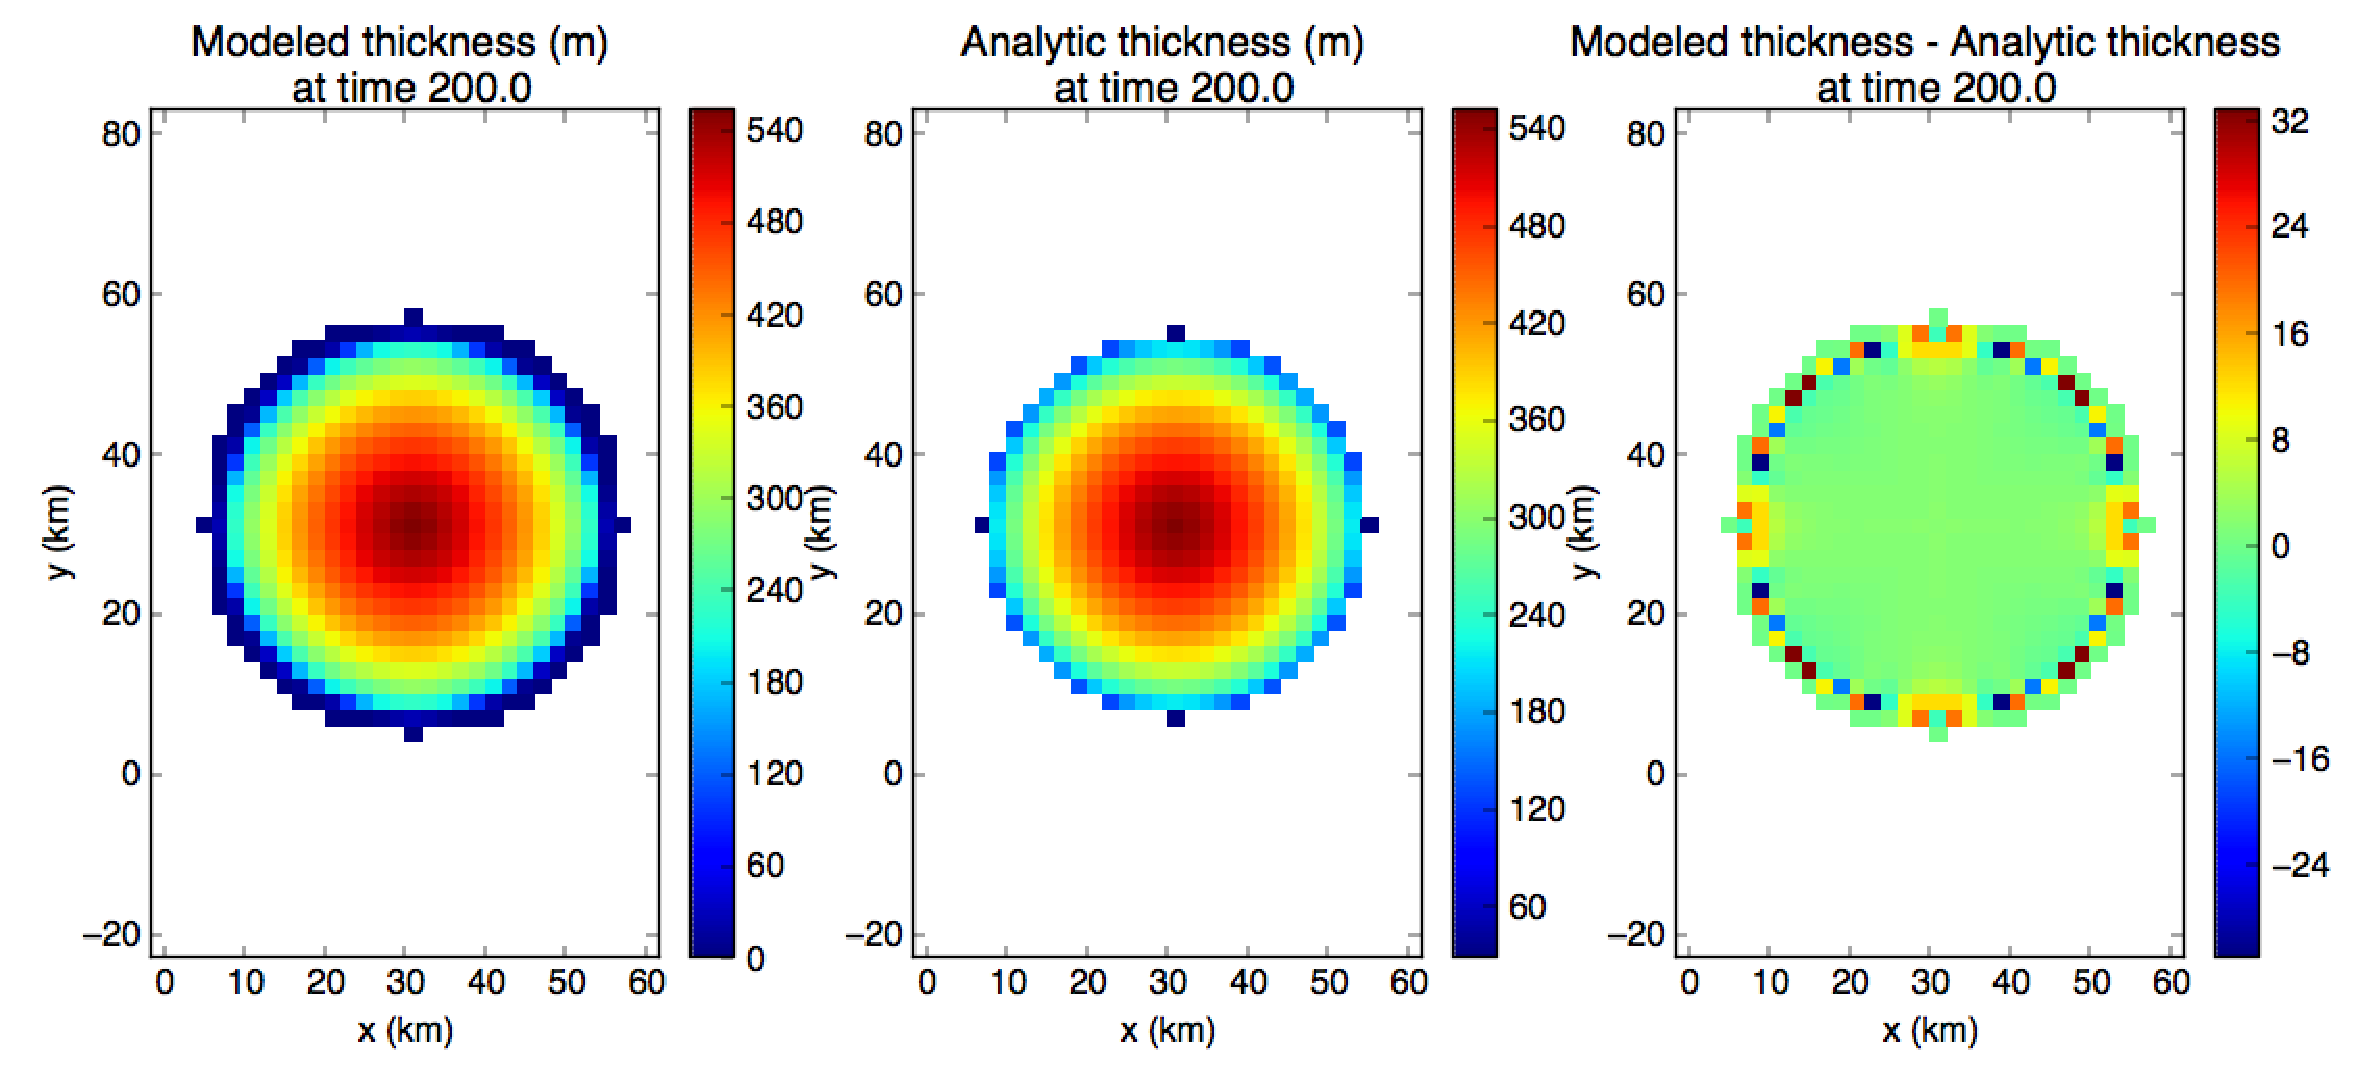
\includegraphics[width=16.4cm]{\dir/halfar_results.eps}
	\caption{Halfar test case results after 200 years of dome evolution. This figure is generated by \texttt{halfar\_results.py}.}
	\label{fig:halfarresults}
\end{figure}


\FloatBarrier


% =====================================
\subsection{EISMINT-1}
% =====================================
\label{sec:eismint_description}
This test case is from phase 1 of the European Ice Sheet Modelling INiTiative intercomparison experiments.  These experiments are described in more detail
\href{http://homepages.vub.ac.be/~phuybrec/eismint.html}{here}\footnote{http://homepages.vub.ac.be/~phuybrec/eismint.html} and in \citet{Huybrechts1996}.

\subsubsection{Provided Files}
\label{subsec:eismint_files}

\begin{itemize}
	\item README \\
	Information about the test case, including technical details about running it.
	\item *.config \\
  	There are six .config files for each of the six experiments in EISMINT 1.  There are three fixed margin experiments (fm) and three moving margin experiments (mm).
\end{itemize}

\subsubsection{Running the test}
There is not a script for running these experiments, they are simply run manually, e.g. using: 

\texttt{./cism\_driver e1-fm.1.config}

\subsubsection{Results}
\label{subsecc:eismint_results}
These experiments are meant to be run to steady-state, and the supplied .config files are setup to run for long enough for it to be reached.
These simulations take more than a few minutes to complete.
As the initial ice sheet evolves, its shape eventually reaches a steady-state with the imposed surface mass balance.  Currently there is not a script for analyzing the CISM results.  However, users can visually compare their results to those in the \citet{Huybrechts1996} paper.


% =====================================
\subsection{EISMINT-2}
% =====================================
\label{sec:eismint2_description}
This test case is from phase 2 of the European Ice Sheet Modelling INiTiative intercomparison experiments.  These experiments are described in more detail
\href{http://homepages.vub.ac.be/~phuybrec/eismint.html}{here}\footnote{http://homepages.vub.ac.be/~phuybrec/eismint.html} and in \citet{Payne2000}.

\subsubsection{Provided Files}
\label{subsec:eismint2_files}

\begin{itemize}
	\item README \\
	Information about the test case, including technical details about running it.
  	\item *.config \\
  	There are 11 .config files for each of the a-f experiments in EISMINT-2.
  	\item mound.nc, trough.nc \\
    	These are input netCDF files used by the EISMINT-2 experiments.
\end{itemize}

\subsubsection{Running the test}
There is not a script for running these experiments, they are simply run manually, e.g. using: 

\texttt{./cism\_driver e2.a.config}


\subsubsection{Results}
\label{subsecc:eismint2_results}
These experiments are meant to be run to steady-state, and the supplied .config files are setup to run for long enough for it to be reached.  
Note that some of the experiments use the final state of a previous experiment 
as the initial condition (e.g., most experiments following experiment A use the final steady-state from A as an initial condition).  
See the experimental descriptions in \citet{Payne2000} for details.
These simulations take more than a few minutes to complete.
As the initial ice sheet evolves, its shape eventually reaches a steady-state with the imposed surface mass balance.  Currently there is not a script for analyzing the CISM results.  However, users can visually compare their results to those in the \citet{Payne2000} paper.


% =====================================
\subsection{GLINT example}
% =====================================
\label{sec:glint_example}

\textbf{ *** Glint example description needed here; additional details needed below *** }

\subsubsection{Provided Files}

\begin{itemize}
	\item README \\
		Information about the test case, including technical details about running it.
\item ?.config \\
  ???
\item ???... \\
\end{itemize}

\subsubsection{Running the test}
There is not a script for running this experiment.  It must be run manually, e.g.: 

\texttt{./cism\_driver greenland\_20km.config glint\_example.config}

[describe the two .config syntax]

\subsubsection{Results}
???




% =====================================

\section{Higher-Order Test Cases}
\label{sc:ho-tests}

The higher-order test cases are designed to test various aspects of higher-order dycores.
By default they all currently use the GLISSADE dycore.  Other higher-order dycores can be applied
to these same tests as they become available and additional test cases will be added as needed.

% =====================================
\subsection{Dome}
% =====================================
The ``Dome'' test case is based on a parabolic dome of ice, similar to the Halfar dome test case.
By default the Dome has the same radius and the same center thickness as the Halfar case.
However, it uses a simple square root function for defining thickness as a function 
of distance from the dome center, which results in a somewhat steeper profile.  
The Dome has been a primary test used for day-to-day testing of higher-order
test cases because it is simple and relatively fast to run.  It is a good test
to confirm that basic higher-order model physics is working correctly, but does
not strenuously test the model physics, a range of boundary conditions, or analytically verify the model.

\subsubsection{Provided Files}

\begin{itemize}
	\item README \\
		Information about the test case, including technical details about running it.
	\item dome.py \\
		The script to setup and run the test test.
 	 \item dome.config \\
  		The default configuration settings for running CISM with the test case.
	\item dome.forcing.py \\
		A optional script for setting up an example of a CISM time-dependent forcing file.
  	\item dome.forcing.config \\
  		An example configuration script that can be used to run CISM with the forcing file
  		generated by \texttt{dome.forcing.py}
\end{itemize}

\subsubsection{Running the test}
One script sets up the initial condition and runs the model:

\texttt{./dome.py}

There is not a script for analyzing the results.

\textit{Optional:  Time-dependent forcing example}

The Dome test case can be used to setup an example of how to use CISM's time-dependent
forcing capability.  (See Section \ref{ug.sec.config} for more details about time-dependent
forcing.)  To create a forcing file with some time-varying (though arbitrary) forcing, run:

\texttt{./dome.forcing.py}

Then you can run the model using the \texttt{dome.forcing.config} configuration file:

\texttt{./dome.py -c dome.forcing.config}

or

\texttt{./cism\_driver dome.forcing.config}


\subsubsection{Results}
There is not an analytic solution for this test, nor is there a script to analyze
the results.  You can manually inspect the results using a tool such as \texttt{ncview}.\footnote{See section \ref{sec:install-netcdf}}
Sample output is shown in Figure \ref{fig:domeresults}.
\begin{figure}[H!]
	\centering
	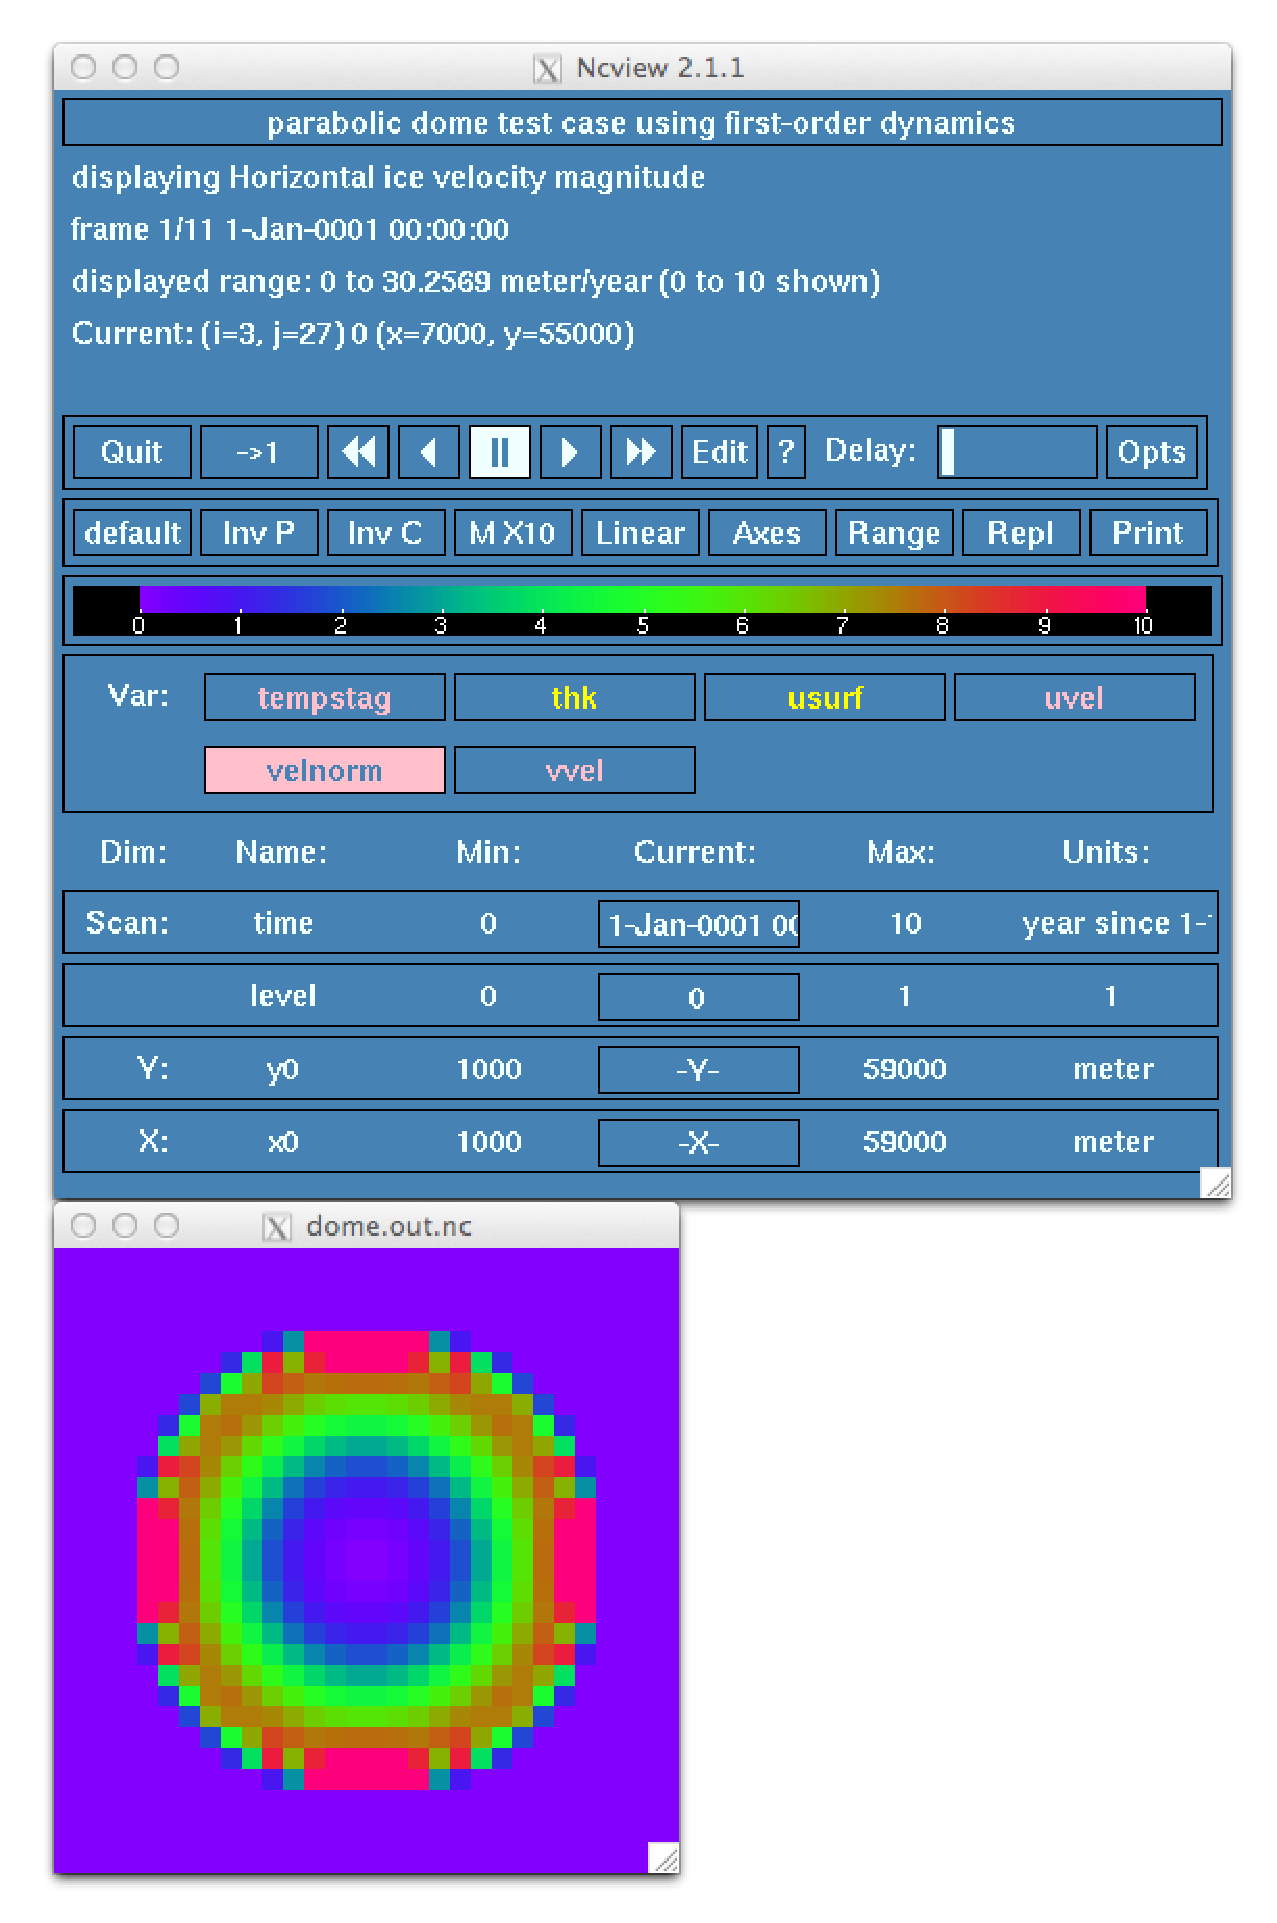
\includegraphics[width=7.0cm]{\dir/dome-output.eps}
	\caption{Dome velnorm (i.e., the ice speed in m/yr) field at time 0 using default \texttt{dome.config} settings. This figure is a screenshot of ncview.}
	\label{fig:domeresults}
\end{figure}
\FloatBarrier

% =====================================
\subsection{ISMIP-HOM}
% =====================================
The Ice Sheet Model Intercomparison Project for Higher-Order Models (ISMIP-HOM)
prescribes a set of experiments meant to test the implementation of higher-order physics.  
For more information, see \href{http://homepages.ulb.ac.be/~fpattyn/ismip/}{here}
\footnote{http://homepages.ulb.ac.be/~fpattyn/ismip/} and the ISMIP-HOM description paper by \citet{Pattyn2008}.

The python scripts provided (runISMIPHOM.py and plotISMIPHOM.py, refered to in the following as the ISMIP-HOM 
scripts) were created to run experiments A through F using CISM and compare the results with results from other models. 

Note: The \texttt{README} file describes many additional details about running and analyzing the
test case that are not described here.

\subsubsection{Provided Files}

\begin{itemize}
	\item README \\
		Information about the test case, including technical details about running it.
	\item ishom.config \\
		A default configuration file used as a template for generating the .config file for each test.
    		If you wish to run the tests with different solver settings, for example, you should edit this file.
	\item runISMIPHOM.py \\
		The script used for running any/all of the ISMIP-HOM experiments.  
    		Invoke with `- - help' to see the many command line options for controlling execution.
  \item plotISMIPHOM.py \\
		The script used for analyzing/plotting any/all of the ISMIP-HOM experiments.  
    		Invoke with `- - help' to see the many command line options for controlling execution.
\end{itemize}

\subsubsection{Running the test}
One script sets up the initial condition and runs the model:

\texttt{./runISMIPHOM.py}

and another is used to analyze the results:

\texttt{./plotISMIPHOM.py}

\subsubsection{Results}
The \texttt{plotISMIPHOM.py} script will plot results relative to other models.
None of the ISMIP-HOM tests have a useful analytic solution, so these tests are
used as community benchmarks rather than actual model verification tests.
Therefore, the \citet{Pattyn2008} paper is useful for intepreting model results.
An example output plot is shown in Figure \ref{fig:ismiphom-results}.

\begin{figure}[H!]
	\centering
	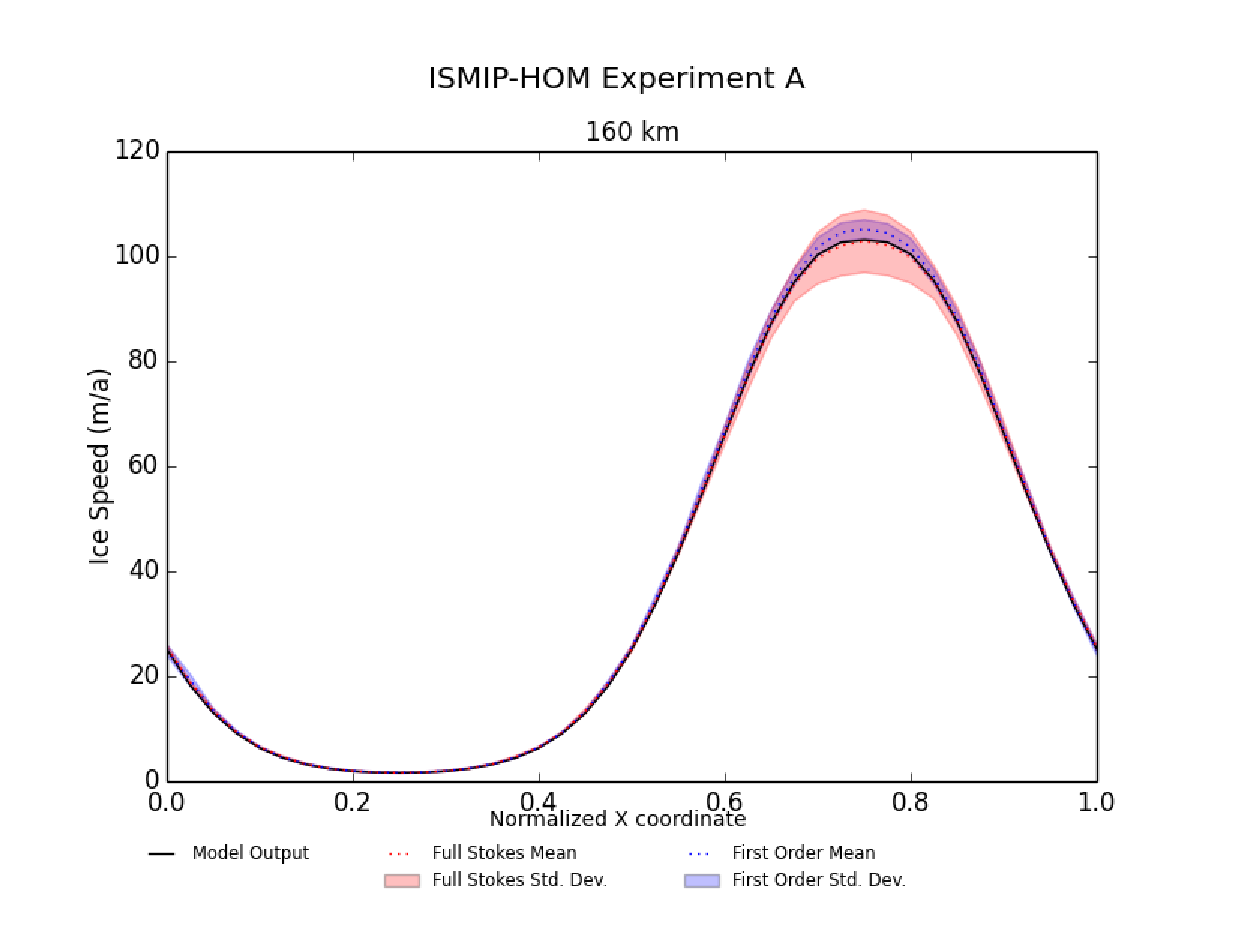
\includegraphics[width=10.0cm]{\dir/ISMIP-HOM-A-cis1.eps}
	\caption{An example of the ISMIP-HOM test case output for test A at size L=160 km. 
CISM output is shown with black line and the range of output from other models is shown by colored bars. 
This figure was generated with \texttt{./plotISMIPHOM.py -e a -s 160} after running the test with \texttt{./runISMIPHOM.py -e a -s 160}.
Additional options (e.g., running and plotting for multiple tests simultaneously) are described in the \texttt{README} and by invoking the
`- - help' option at the command line.}
	\label{fig:ismiphom-results}
\end{figure}
\FloatBarrier

% =====================================
\subsection{Stream}
% =====================================

This test case simulates flow over an idealized ice stream underlain by a subglacial till with a known and specified
yield stress distribution (also, see discussion in Section \ref{sc:higher-order-bcs}). For the two distributions available in this test case, 
analytical solutions are available from \citet{Raymond2000} and \citet{Schoof2006}. 

For the Raymond test case, the yield stress within the ice stream is given a uniform value below the driving stress, and outside of the
ice stream it is given a uniform value much higher than the driving stress (i.e., the yield stress distribution is approximated by a
``step" function). For the Schoof test case, the till yield stress across the ice stream is given by a continuously varying function.

In both cases, the basal properties vary in the across-flow direction only and are symmetric about the ice stream centerline.
As a result, the velocity solutions are also uniform along flow and symmetric about the centerline.

\subsubsection{Provided Files}

\begin{itemize}
	\item README \\
		Information about the test case, including technical details about running it.
	\item runStream.py \\
		The script to setup and run the test test.
	\item stream.config.in \\
  The default configuration settings for running CISM with the test case. Note that this
  file is parsed by the runStream.py script. Most of the relevant options that might be changed
  for this test case (e.g., grid spacing) can be done so from the command line, without having to
  edit the .config files (use \texttt{./runStream.py --help} to obtain a description of available options.
  The choice of test case - using the Raymond or Schoof yield stress distribution -  can be toggled 
  by editing line 15 of the runStream.py script.
\end{itemize}

\subsubsection{Running the test}
One script sets up the initial condition and runs the model:

\texttt{./runStream.py}

and another is used to analyze the results:

\texttt{./plotStream.py}

\subsubsection{Results}
The \texttt{plotStream.py} script will plot model output relative to the analytical solutions
given in \citet{Raymond2000} and \citet{Schoof2006}. The choice of analytical solution to compare
to is decided on automatically, based on what value is currently active in the runStream.py script. 
Example output for both test cases is shown in Figure \ref{fig:stream-results}.
	
\begin{figure}[H!]
  \begin{center}
	\includegraphics[width=10.0cm]{\dir/stream_raymond.eps}
	\includegraphics[width=10.0cm]{\dir/stream_schoof.eps}
  \end{center}
  \caption{Comparison between CISM model output (black) and analytic solution (red) for the Raymond (top) and Schoof (bottom) stream test cases. This figure was generated with \texttt{./plotStream.py} after running the test with \texttt{./runStream.py}.
Additional runtime options are described in the \texttt{README} and by invoking the `- - help' option at the command line.}
  \label{fig:stream-results}
\end{figure} 

% =====================================
\subsection{Confined Shelf}
% =====================================
This test setup is from tests 3 and 4 from the idealized (i.e. not Ross) EISMINT-shelf test 
cases.  It simulates the flow within an idealized, 500 m thick ice shelf in a 
confined, rectangular embayment.  Grounded ice is not explicitly modeled but included in the 
model setup as Dirichlet boundary conditions for velocity along the ice shelf edges.
More detailed information on this test case can be found 
\href{http://homepages.vub.ac.be/~phuybrec/eismint/iceshelf.html}{here}
\footnote{http://homepages.vub.ac.be/~phuybrec/eismint/iceshelf.html} in the 
``shelf-descr.pdf" document.

Note that the Confined Shelf and Circular Shelf experiments are both in the 
\texttt{tests/higher-order/shelf} directory and share some files.

\subsubsection{Provided Files}

\begin{itemize}
	\item README \\
		Information about the test case, including technical details about running it.
	\item confined-shelf.py \\
		The script to setup and run the test test.
	\item confined-shelf.config \\
  The default configuration settings for running CISM with the test case.
\end{itemize}

\subsubsection{Running the test}
One script sets up the initial condition and runs the model:

\texttt{./confined-shelf.py}

\subsubsection{Results}
There is not a script for analyzing the results.  See the URL above for information 
about assessing the model output.
You can manually inspect the results using a tool such as \texttt{ncview}.
An example is shown in Figure \ref{fig:confinedshelf-results}.

\begin{figure}[H!]
	\centering
	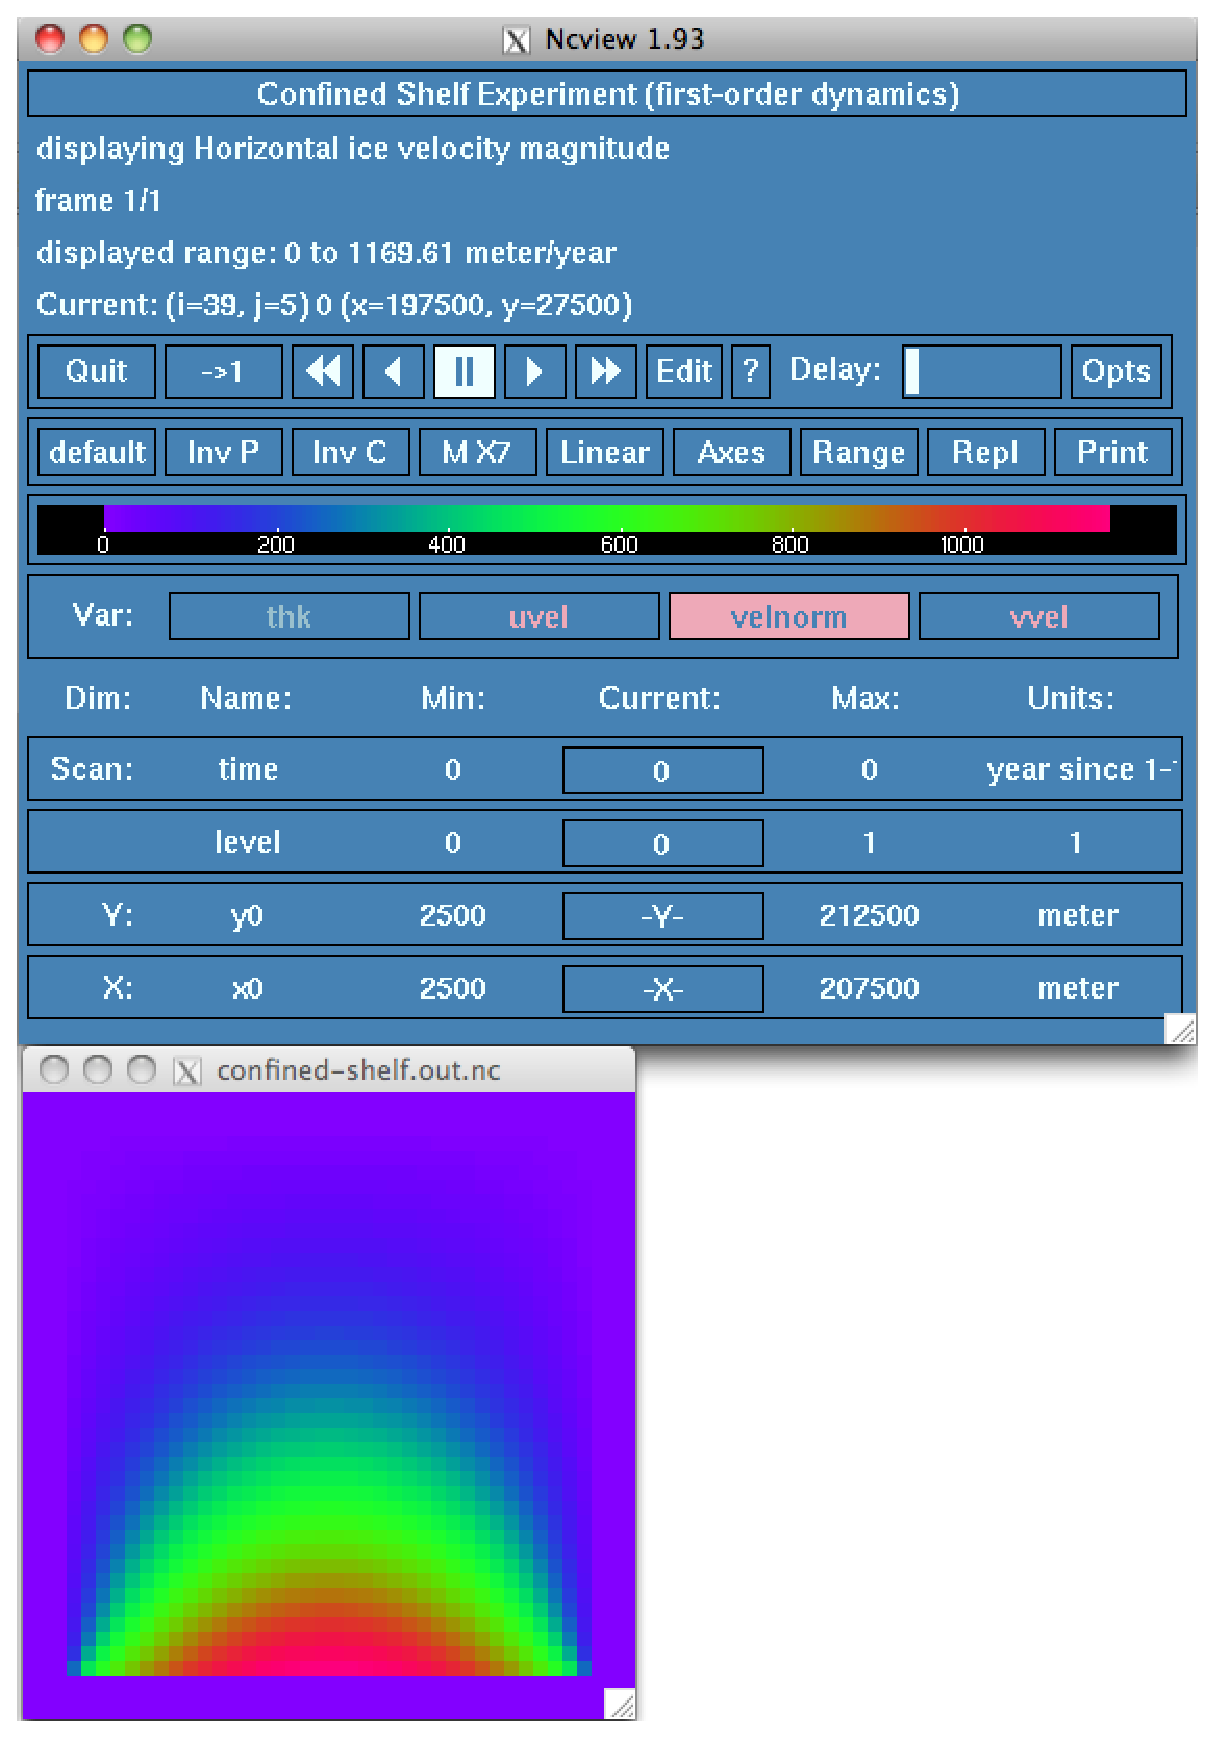
\includegraphics[width=8.0cm]{\dir/confinedshelf-output.eps}
	\caption{Confined shelf velnorm field using default \texttt{confined-shelf.config} settings. This figure is a screenshot of ncview.}
	\label{fig:confinedshelf-results}
\end{figure}
\FloatBarrier

% =====================================
\subsection{Circular Shelf}
% =====================================
This test is a variant on the confined shelf test case discussed above. It simulates the flow within a circular ice shelf with a uniform thickness
of 1000 m, which is grounded at a single grid point at its center. This test case confirms a working ``floating ice" boundary condition implementation
in two dimensions (i.e, in map plane view) and also confirms radial symmetry. 

Note that the Confined Shelf and Circular Shelf experiments are both in the 
\texttt{tests/higher-order/shelf} directory and share some files.

\subsubsection{Provided Files}

\begin{itemize}
	\item README \\
		Information about the test case, including technical details about running it.
	\item circular-shelf.py \\
		The script to setup and run the test test.
	\item circular-shelf.config \\
  The default configuration settings for running CISM with the test case.
\end{itemize}

\subsubsection{Running the test}
One script sets up the initial condition and runs the model:

\texttt{./circular-shelf.py}

\subsubsection{Results}
There is not a script for analyzing the results.
You can manually inspect the results using a tool such as \texttt{ncview}.
An example is shown in Figure \ref{fig:circularshelf-results}.

\begin{figure}[H!]
	\centering
	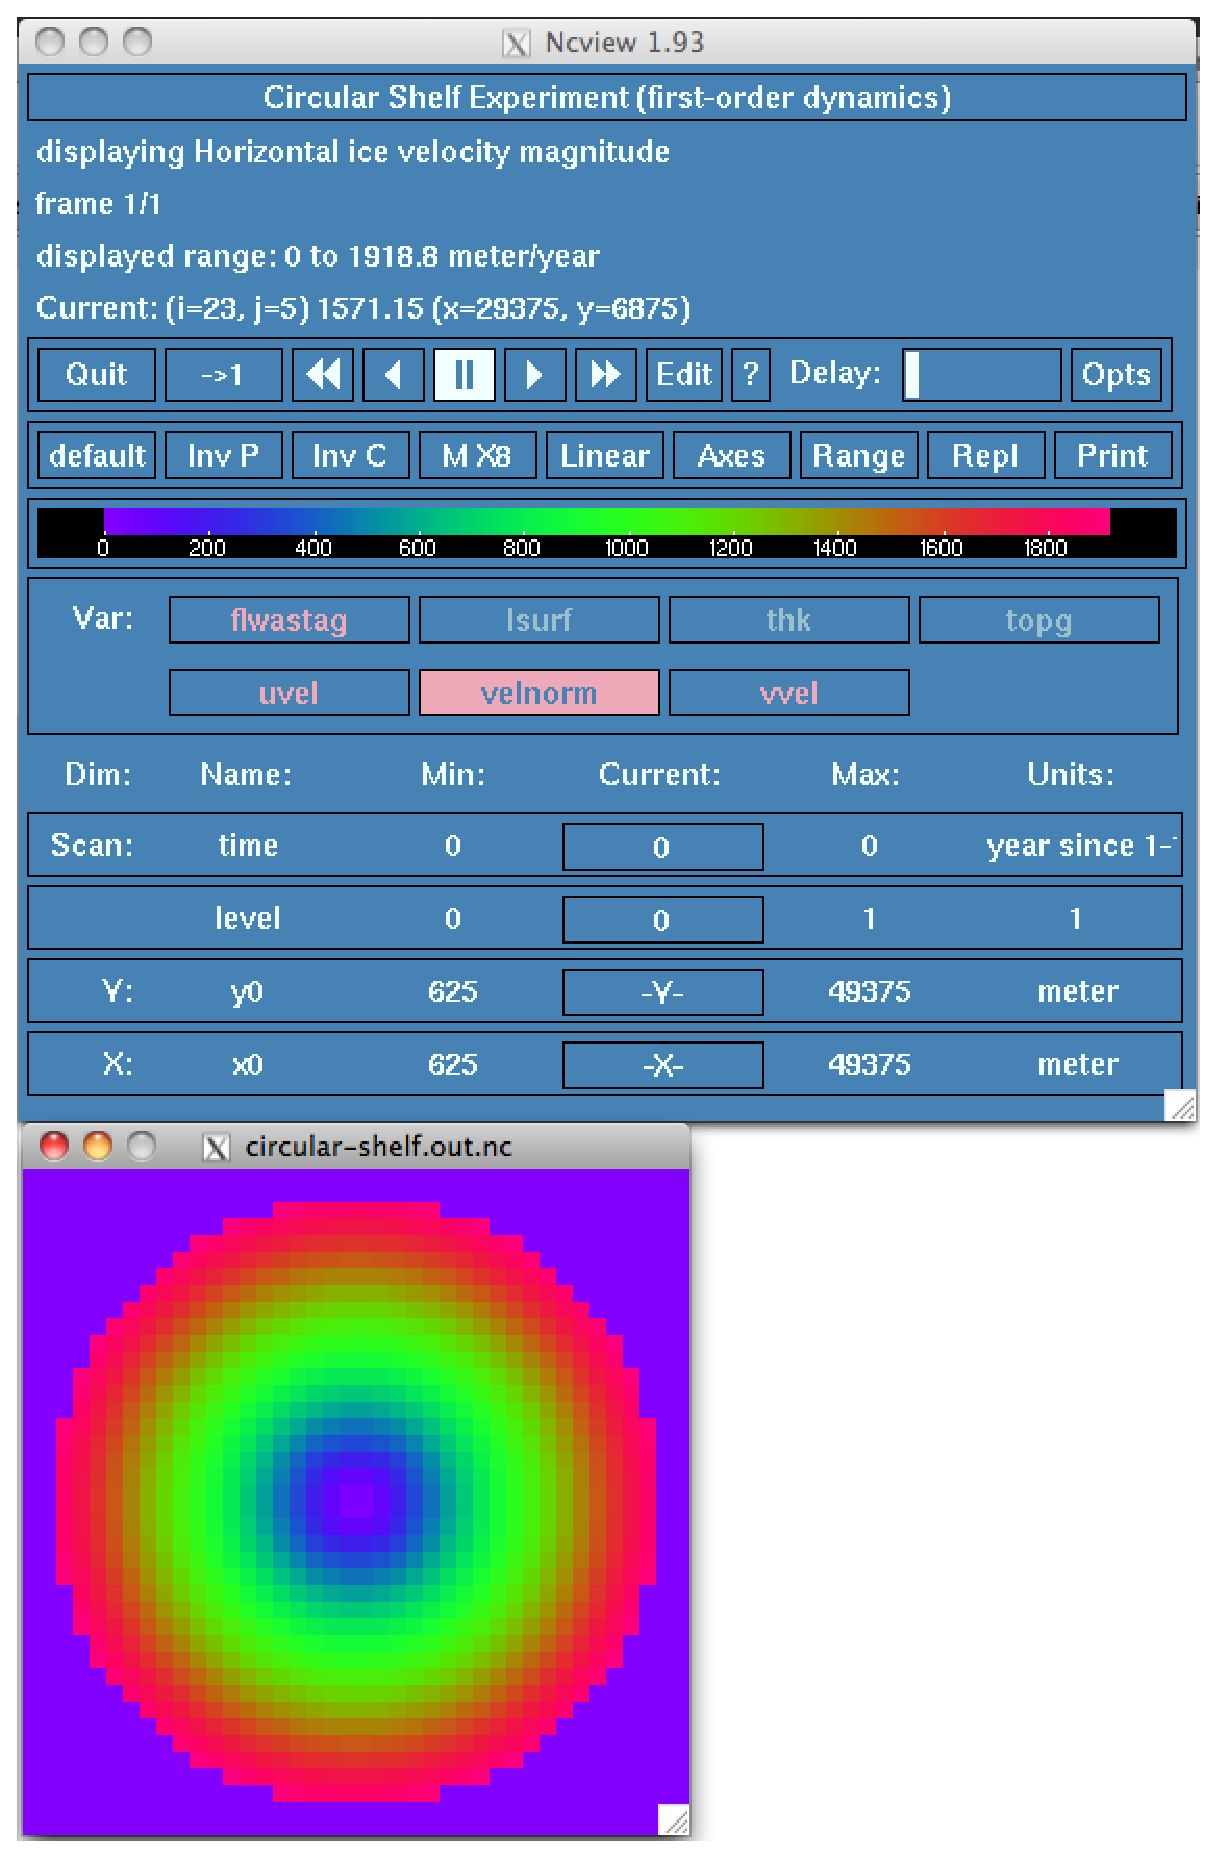
\includegraphics[width=8.0cm]{\dir/circularshelf-output.eps}
	\caption{Circular shelf velnorm field using default \texttt{circular-shelf.config} settings. This figure is a screenshot of ncview.}
	\label{fig:circularshelf-results}
\end{figure}
\FloatBarrier

% =====================================
\subsection{Ross Ice Shelf}
% =====================================
This experiment was designed to simulate the flow of the Ross Ice Shelf of Antarctica under idealized conditions (e.g., constant and uniform
flow-law rate factor). For more information about the experiment and its results see 
\href{http://homepages.vub.ac.be/~phuybrec/eismint/iceshelf.html}{here}\footnote{http://homepages.vub.ac.be/~phuybrec/eismint/iceshelf.html}. 
Also, see \citet{MacAyeal:1996vn} for a discussion of the official model intercomparison results.

This experiment will typically take about 10 minutes to run on a single processor.

\subsubsection{Provided Files}

\begin{itemize}
	\item README \\
		Information about the test case, including technical details about running it.
	\item runRoss.py \\
		The script to setup and run the test test.
	\item ross.config \\
  The default configuration settings for running CISM with the test case.
	\item plotRoss.py \\
		The script to plot the test results.
\end{itemize}

\subsubsection{Running the test}
One script sets up the initial condition and runs the model:

\texttt{./runRoss.py}

and another can be used to visualize the results:

\texttt{./plotRoss.py}

\subsubsection{Results}
The \texttt{plotRoss.py} script will generate a figure of the velocity field
calculated for the Ross Ice Shelf.  The results should look very similar to Figures \ref{fig:rossresults1} and \ref{fig:rossresults2}. You can
compare these with similar figures in the paper by \citet{MacAyeal:1996vn}.

\begin{figure}[H!]
	\centering
	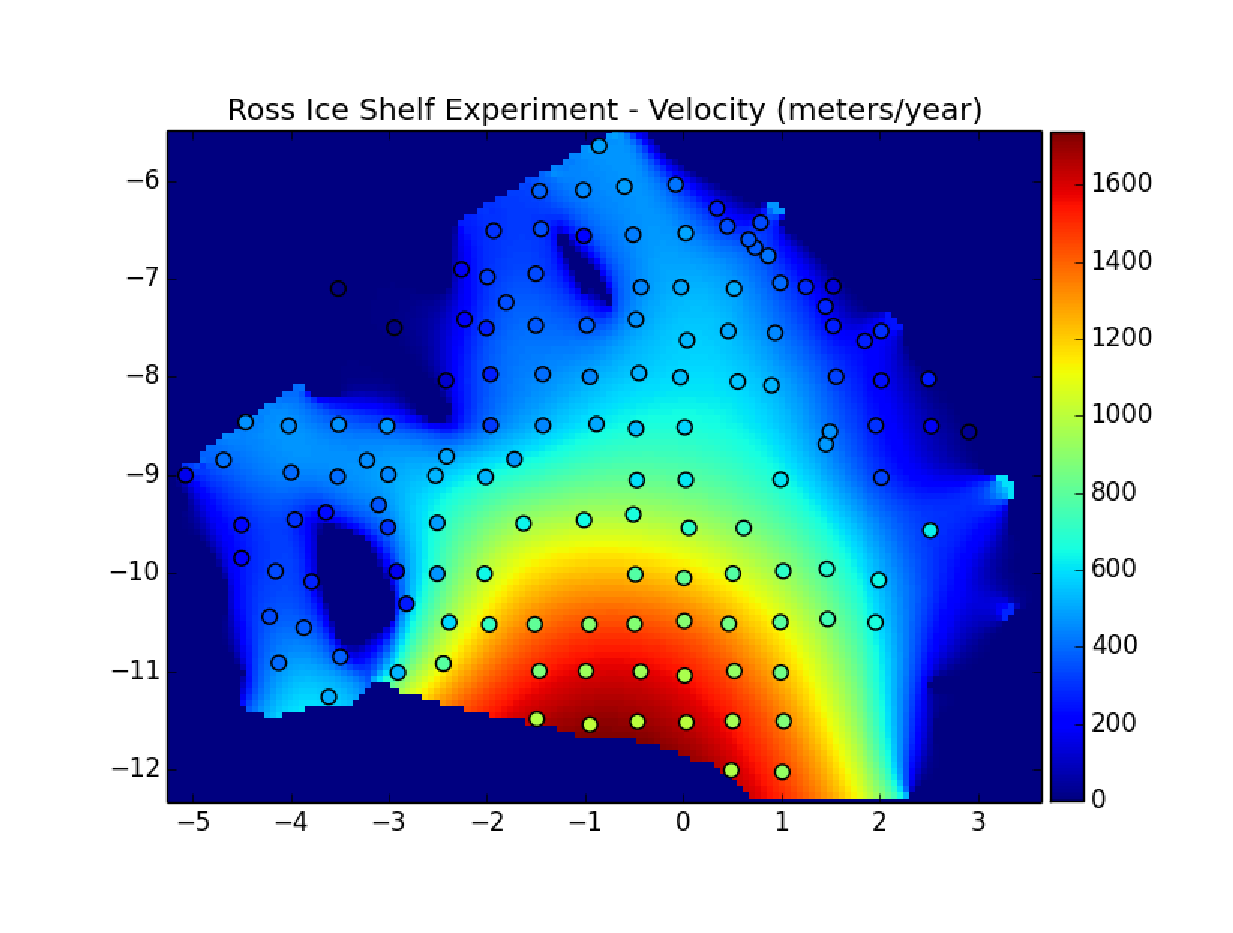
\includegraphics[width=10.0cm]{\dir/RossModelVelField.eps}
	\caption{Ross Ice Shelf velocity field calculated by CISM. This figure is generated by \texttt{plotRoss.py}.}
	\label{fig:rossresults1}
\end{figure}
%\FloatBarrier

\begin{figure}[H!]
	\centering
	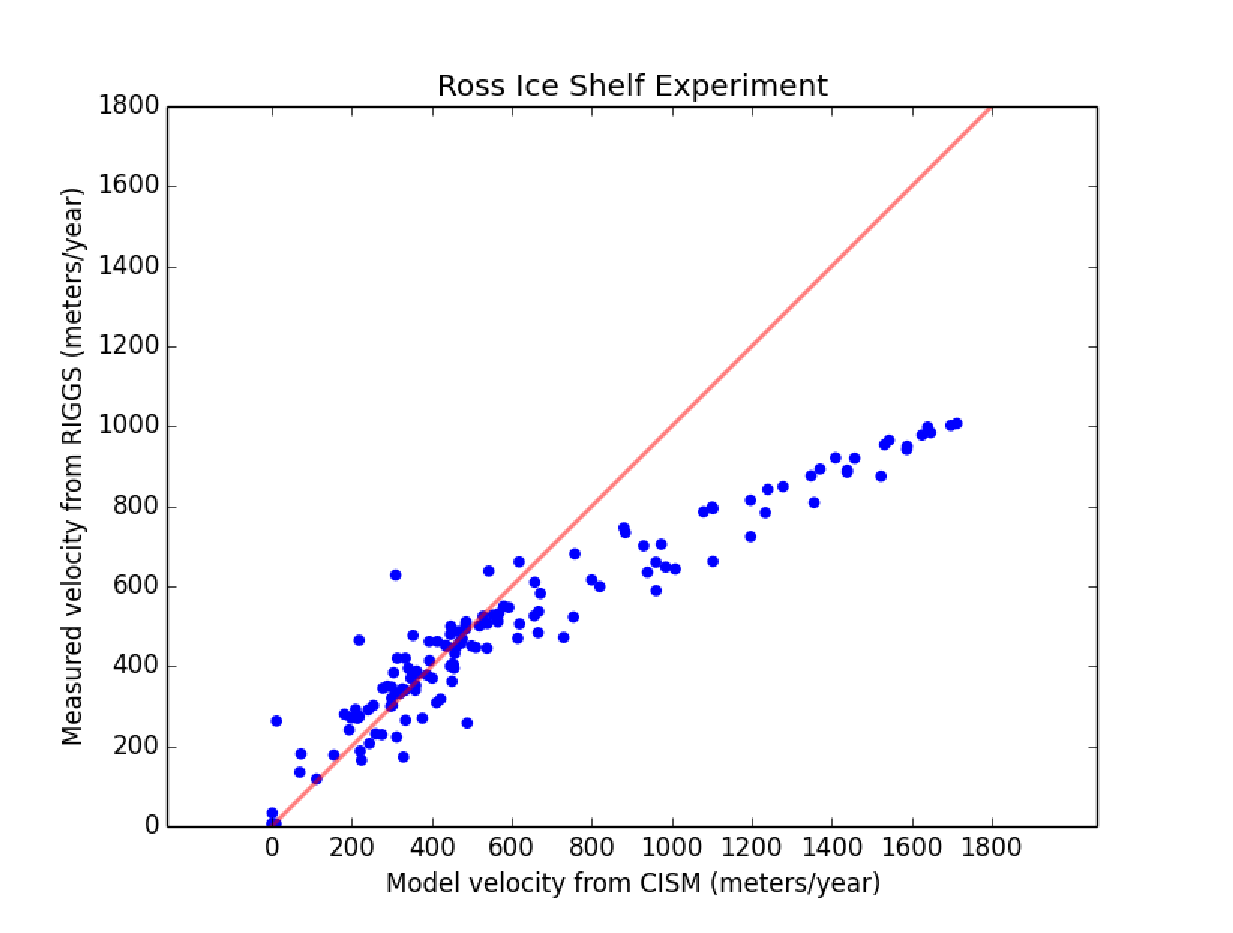
\includegraphics[width=10.0cm]{\dir/RossModelvsObs.eps}
	\caption{CISM-modeled Ross Ice Shelf speeds vs. those from observations. This figure is generated by \texttt{plotRoss.py}.}
	\label{fig:rossresults2}
\end{figure}
\FloatBarrier


% =====================================
\subsection{Other Tests}
% =====================================
Additional higher-order tests that are still in development (e.g., ``slab" and ``stream") are also included in the \texttt{./tests/higher-order/}
directory. Instructions for how to run these tests are included in each directory. However, since these tests have not yet been validated yet, 
they are for use at your own risk.






%% Old documentation below here
\chapter{ \Large *** NOTE: below here, the documentation is simply a copy of the old documentation, with edits as noted ***}

\chapter{User Guide}
\renewcommand{\dir}{ug}
This package provides an addon library to \href{http://developer.berlios.de/projects/glimmer-cism/}{Glimmer-CISM} which provides a bedrock erosion and sediment transport component. Drivers are provided for EISMINT type forcing and the EIS driver. You can use \texttt{erosion} with your own climate drivers (see Section \ref{erosion.sec.using_it}).

\section{Model Configuration}
Add a selection of the follwing configuration options to your GLIDE configuration file to enable and control erosion and sediment transport.
\begin{center}
  \tablefirsthead{%
    \hline
  }
  \tablehead{%
    \hline
    \multicolumn{2}{|l|}{\emph{\small continued from previous page}}\\
    \hline
  }
  \tabletail{%
    \hline
    \multicolumn{2}{|r|}{\emph{\small continued on next page}}\\
    \hline}
  \tablelasttail{\hline}
  \begin{supertabular*}{\textwidth}{@{\extracolsep{\fill}}|l|p{9cm}|}
    \hline
    \multicolumn{2}{|l|}{\texttt{[Erosion]}}\\
    \hline
    \multicolumn{2}{|p{0.95\textwidth}|}{Switch on hard bedrock erosion.}\\
    \hline
    \texttt{hb\_erosion} & set parameterisation of hard bedrock erosion\\
    \texttt{ntime} & update erosion calculation every \texttt{ntime} time steps\\
    \texttt{updeate\_topo} & whether erosion/sediment transport changes ice bed topography (default :1)\\
    \hline
    \hline
    \multicolumn{2}{|l|}{\texttt{[Basic\_Transport]}}\\
    \hline
    \multicolumn{2}{|p{0.95\textwidth}|}{Sediment transport is paramterised by assuming transport velocities are proportional to basal ice velocities (see Section \ref{erosion.sec.basic_trans})}\\
    \hline
    \texttt{deformable\_velo} & basal ice velocities are multiplied with this factor to get sediment transport velocities.\\
    \texttt{dirty\_ice\_thick} & thickness of dirty basal ice layer\\
    \texttt{soft\_a},  \texttt{soft\_b}& parameterisation of maximum deformable sediment layer thickness, $$z_{\text{max}}=a+b|\vec{\tau}_b|$$\\
    \hline
    \hline
    \multicolumn{2}{|l|}{\texttt{[Transport]}}\\
    \hline
    \multicolumn{2}{|p{0.95\textwidth}|}{Deforming sediment layer is based on some rheology (see Section \ref{erosion.sec.full_trans}).}\\
    \hline
    \texttt{dirty\_ice\_thick} & thickness of dirty basal ice layer\\
    \texttt{calc\_btrc} & sediment velocities set ice sliding velocities.\\
    \texttt{effective\_pressure} & set the effective pressure at the ice base.\\
    \texttt{pressure\_gradient} & set pressure gradient in sediment bed.\\
    \texttt{phi} & angle of internal friction, $\phi$.\\
    \texttt{cohesion} & cohesion of sediments.\\
    \texttt{a} & factor for sediment flow law.\\
    \texttt{m} & exponent of effective pressure.\\
    \texttt{n} & exponent of shear stress.\\
  \end{supertabular*}
\end{center}

\section{Using the Library}\label{erosion.sec.using_it}
The \texttt{erosion} module provides a number of subroutines which can be used to add erosion/sediment transport to an ice sheet model based on GLIMMER. Have a look at the EISMINT driver \texttt{simple\_erosion.f90}.

All variables associated with the module are stored in a derived type. Similarly to GLIDE you will need to declare a variable of that derived type:
\begin{verbatim}
type(erosion_type) :: er
\end{verbatim}
The erosion component is initialised after GLIDE was initialised using the call
\begin{verbatim}
call er_initialise(er,config,model)
\end{verbatim}
The erosion time step is done after the first GLIDE timestep:
\begin{verbatim}
call glide_tstep_p1(model,time)
call er_tstep(er,model)
\end{verbatim}
Finally, the model is shut down before GLIDE is shut down with
\begin{verbatim}
call er_finalise(er)
\end{verbatim}

%\section{Visualisation}\label{erosion.sec.vis_it}
%\texttt{erosion} comes with a number of python scripts for visualising sediments.
%
%\begin{pycf}{plot\_seds.py -T-1 -pprof --not\_p  fenscan.nc sediments.ps}{\dir/figs/sediments.eps}
%plots a map of sediment erosion/deposition of the last time slice. The \texttt{-p} option together with the \texttt{--not\_p} option plots the profile. This program plots sediment erosion/deposition relative to the initial sediment distribution. Blue areas indicate areas where sediments have been removed. Red areas indicate areas where sediments have been deposited.
%\end{pycf}
%
%\begin{pycf}{plot\_seds\_profile.py -t0. -e stages -pprof --not\_p fenscan.nc prof.ps}{\dir/figs/sed_profile.eps}
%plots a profile showing sediment erosion/deposition. A file containing timings of glacial stages is required. The time when sediments are deposited are indicated with colours found in this file. The \texttt{stages} file contains 4 comma--eparated columns. The first column contains the name, second and thrid column start and end time in years, and the last column a R/G/B triplet for the background colour.
%\end{pycf}


\chapter{Tutorial}
\renewcommand{\dir}{tut}
\newcommand{\dir}{tut}

\pagestyle{myheadings} \markright{GLIMMER {\glimmerver} --- Tutorial}

\begin{document}
\title{GLIMMER {\glimmerver} --- Tutorial}
\author{Felix Hebeler \thanks{fhebeler@geo.unizh.ch}}
\maketitle
\tableofcontents
\newpage

\newcommand{\dir}{tut}

\pagestyle{myheadings} \markright{GLIMMER {\glimmerver} --- Tutorial}

\begin{document}
\title{GLIMMER {\glimmerver} --- Tutorial}
\author{Felix Hebeler \thanks{fhebeler@geo.unizh.ch}}
\maketitle
\tableofcontents
\newpage

\newcommand{\dir}{tut}

\pagestyle{myheadings} \markright{GLIMMER {\glimmerver} --- Tutorial}

\begin{document}
\title{GLIMMER {\glimmerver} --- Tutorial}
\author{Felix Hebeler \thanks{fhebeler@geo.unizh.ch}}
\maketitle
\tableofcontents
\newpage

\input{\dir/tut.tex}
\end{document}

\end{document}

\end{document}


%\part{Developer Documentation}

\chapter{Numerics}
\Large *** NOTE: everything in this section was moved into the current chapter describing the Glide dycore ***
%\renewcommand{\dir}{num}
%This part describes the numerical implementation of GLIMMER in some detail. It is hoped that more parts will be added in the future.
\section{Ice Thickness Evolution}
\label{sc:glide_thickness_evolution}
The evolution of the ice thickness, $H$, stems from the continuity equation and can be expressed as
\begin{equation}
  \label{kin.eq.ice_thickness}
  \frac{\pd H}{\pd t} = -\vec\nabla\cdot(\overline{\vec{u}} H) + B,
\end{equation}
where $\overline{\vec{u}}$ is the vertically averaged ice velocity, $B$ is the surface mass balance and $\vec\nabla$ is the horizontal gradient operator \citep{Payne1997}. 

%For large--scale ice sheet models, the \emph{shallow ice approximation} is generally used. 
For some regions of large--scale ice sheets, such as the slow moving interior, or for simulations run at coarse spatial resolution, a model governed by the \emph{shallow ice approximation} may be appropriate. Further, for very-long time integrations, such as those required in paleoclimate studies, a model governed by the shallow ice approximation may
be the only computationally practical approach.
%The shallow ice approximation assumes that bedrock and ice surface slopes are sufficiently small so that the normal stress components can be neglected \citep{Hutter1983}. 

Based largely on the assumption that bedrock and ice surface slopes are sufficiently small \citep{Hutter1983}, the shallow ice approximation neglects all stress components other than those associated with vertical shearing in the horizontal directions. 
These stresses, $\tau_{xz}$ and $\tau_{yz}$, are approximated by
\begin{equation}
  \label{kin.eq.horiz_shear}
  \begin{split}
    \tau_{xz}(z)&=-\rho g(s-z)\frac{\pd s}{\pd x},\\
    \tau_{yz}(z)&=-\rho g(s-z)\frac{\pd s}{\pd y},
  \end{split}
\end{equation}
where $\rho$ is the density of ice, $g$ the acceleration due to gravity and $s=H+h$ the ice surface. \textbf{Steve: I think the latter should be H + b? Unless they use h in this chapter to denote the bedrock elevation. If that is the case, we should probably update so that it is consistent w/ the rest of the documentation, which uses b for bedrock elev.}

Strain rates $\dot{\epsilon}_{ij}$ of polycrystalline ice are related to the stress tensor by the non--linear flow law:
\begin{equation}
  \label{kin.eq.flowlaw}
  \dot{\epsilon}_{iz}=\frac12\left(\frac{\pd u_i}{\pd z}+\frac{\pd u_z}{\pd i}\right)=A(T^\ast)\tau_\ast^{(n-1)}\tau_{iz}\qquad i=x,y,
\end{equation}
where $\tau_\ast$ is the effective shear stress defined by the second invariant of the stress tensor, $n$ the flow law exponent and $A$ the temperature--dependent flow law coefficient. $T^\ast$ is the absolute temperature corrected for the dependence of the melting point on pressure \cite[$T^\ast=T+8.7\cdot10^{-4}(H+h-z)$, $T$ in Kelvin,][]{Huybrechts1986}. 
%The parameters $A$ and $n$ have to be found by experiment. 
The parameters $n$ and $A$ are determined experimentally; $n$ is usually taken to be 3 and $A$ depends primarily on temperature and secondarily on factors such as crystal
size and orientation and ice impurities. 
%on factors such as temperature, crystal size and orientation, and ice impurities. 
Experiments suggest that $A$ follows the Arrhenius relationship:
\begin{equation}
  \label{kin.eq.arrhenius}
  A(T^\ast)=fae^{-Q/RT^\ast},
\end{equation}where $a$ is a temperature--independent material constant, $Q$ is the activation energy for creep and $R$ is the universal gas constant \citep{Paterson1994}. 
$f$ is a tuning parameter that may be used to ``speed--up" ice flow, accounting for the effects of ice impurities and the development of anisotropic ice fabrics \citep{Payne1999,Tarasov1999,Tarasov2000,Peltier2000}.

Integrating \eqref{kin.eq.arrhenius} with respect to $z$ gives the vertical profile of the horizontal velocity in each column:
\begin{equation}
  \label{kin.eq.horiz_velo}
  \vec u(z)-\vec u(h) = -2(\rho g)^n|\vec\nabla s|^{n-1}\vec\nabla s\int_h^zA(s-z)^ndz,
\end{equation}
where $\vec u(h)$ is the basal velocity (sliding velocity). Integrating \eqref{kin.eq.horiz_velo} again with respect to $z$ gives an expression for the vertically averaged ice velocity:
\begin{equation}
  \label{kin.eq.avg_velo}
  \overline{\vec u}H=-2(\rho g)^n|\vec\nabla s|^{n-1}\vec\nabla s\int_h^s\int_h^zA(s-z)^ndzdz'.
\end{equation}

The vertical ice velocity can be derived from the conservation of mass for an incompressible material:
\begin{equation}
  \label{kin.eq.incompress}
  \frac{\pd u_x}{\pd x} + \frac{\pd u_y}{\pd y} + \frac{\pd u_z}{\pd z} = 0.
\end{equation}
Integrating \eqref{kin.eq.incompress} with respect to $z$ gives the vertical profile of the vertical velocity in each column:
\begin{equation}
  \label{kin.eq.vert_velo}
  w(z)=-\int_h^z\vec\nabla\cdot\vec u(z)dz+w(h),
\end{equation}
with lower, kinematic boundary condition
\begin{equation}
  w(h)=\frac{\pd h}{\pd t}+\vec u(h)\cdot\vec\nabla h+S,
\end{equation}
where $S$ is the melt rate at the ice base given by Equation \eqref{temp.eq.meltrate}. The upper kinematic boundary is given by the surface mass balance and must satisfy:
\begin{equation}
  \label{kin.eq.upper_bc}
  w(s)=\frac{\pd s}{\pd t}+\vec u(s)\cdot\vec\nabla s+B.
\end{equation}
\textbf{Steve: need to replace the h with b in the above expressions and also make sure other notation is consistent w/ the rest of the documentation.}

\subsection{Numerical Grid}\label{num.sec.grid}
The continuous equations describing ice physics have to be discretized in order to be solved by a computer (which is inherently finite). This section describes the finite--difference grids used by the model.
\subsubsection{Horizontal Grid}
The modelled region ($x\in[0,L_x]$, $y\in[0,L_y]$) is discretized using a regular grid so that $x_i=(i-1)\Delta x$ for $i\in[1,N]$ (and similarly for $y_j$). The model uses two staggered horizontal grids in order to improve stability. Both grids use the same grid spacing, $\Delta x$ and $\Delta y$, but are offset by half a grid cell (see Fig. \ref{kin.fig.grid}). 
\begin{figure}[htbp]
  \begin{center}
    
\includegraphics{\dir/figs/grid.eps}
    \caption{Horizontal Grid.}
    \label{kin.fig.grid}
  \end{center}
\end{figure}
Quantities calculated on the staggered $(r,s)$--grid are denoted with a tilde, i.e., $\tilde{F}$. Quantities are transformed between grids by averaging over the surrounding nodes; i.e., a quantity in the $(i,j)$--grid becomes in the $(r,s)$--grid:
\begin{subequations}
  \begin{align}
    \tilde{F}_{r,s}&=\tilde{F}_{i+\frac12,j+\frac12}=\frac14(F_{i,j}+F_{i+1,j}+F_{i+1,j+1}+F_{i,j+1}),\\
    \intertext{and similarly for the reverse transformation:}
    F_{i,j}&=F_{r-\frac12,s-\frac12}=\frac14(\tilde{F}_{r-1,s-1}+\tilde{F}_{r,s-1}+\tilde{F}_{r,s}+\tilde{F}_{r-1,s}).
  \end{align}
\end{subequations}

In general, horizontal velocities and associated quantities like the diffusivity are calculated on the $(r,s)$--grid. Ice thickness, temperatures and vertical velocities are calculated on the $(i,j)$--grid.

Horizontal gradients are calculated on the $(r,s)$--grid; i.e., surface gradients are
\begin{subequations}
\begin{align}
  \left(\frac{\pd s}{\pd x}\right)_{r,s}=\tilde{s}^x_{r,s}&=\frac{s_{i+1,j}-s_{i,j}+s_{i+1,j+1}-s_{i,j+1}}{2\Delta x},\\
  \left(\frac{\pd s}{\pd y}\right)_{r,s}=\tilde{s}^y_{r,s}&=\frac{s_{i,j+1}-s_{i,j}+s_{i+1,j+1}-s_{i+1,j}}{2\Delta y}.
\end{align}  
\end{subequations}
Ice thickness gradients, $\tilde{H}^x_{r,s}$ and $\tilde{H}^y_{r,s}$, are formed analogously. Gradients in the $(r,s)$--grid are formed in a similar way: 
\begin{equation}
  \left(\frac{\pd u}{\pd x}\right)_{i,j}=u^x_{i,j}=\frac{\tilde{u}_{r,s-1}-\tilde{u}_{r-1,s-1}+\tilde{u}_{r,s}-\tilde{u}_{r-1,s}}{2\Delta x}.
\end{equation}

\subsubsection{Periodic Boundary Conditions}
The model can be run with horizontal periodic boundary conditions, i.e. with the western edge of the modelled region joined to the eastern edge. Figure \ref{num.fig.grid_ew} illustrates the numeric grid when the model is run in torus mode.

\begin{figure}[htbp]
  \centering
  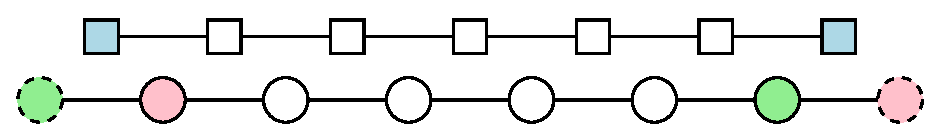
\includegraphics[width=0.9\textwidth]{\dir/figs/grid_ew.eps}
  \caption{A row of the numeric grid when the model is used in torus mode. Circles indicate points in $(i,j)$--grid and squares indicate points in the $(r,s)$--grid. Points with the same color are logically the same.}
  \label{num.fig.grid_ew}
\end{figure}

These boundary conditions are enforced by exchanging points for the temperature and vertical velocity calculations. The ice thicknesses are calculated explicitly at the ghostpoints.

\subsubsection{$\sigma$--Coordinate System}\label{num.sec.sigma}
The vertical coordinate, $z$, is scaled by the ice thickness analogous to the $s$--coordinate in numerical weather simulations \citep[e.g.,][]{Holton1992}. A new vertical coordinate, $\sigma$, is introduced so that the ice surface is at $\sigma=0$ and the ice base at $\sigma=1$ (see Fig. \ref{kin.fig.scale}), i.e.
\begin{equation}
  \label{kin.eq.vertical_scale}
  \sigma=\frac{s-z}{H}.
\end{equation}

\begin{figure}[htbp]
  \begin{center}
    
\includegraphics{\dir/figs/scale.eps}
    \caption[Vertical scaling of the ice sheet model.]{Vertical scaling of the ice sheet model. The vertical axis is scaled to unity. The horizontal coordinates are not changed.}
    \label{kin.fig.scale}
  \end{center}
\end{figure}


The derivatives of a function $f$ in $(x,y,z,t)$ become in the new $(\tilde{x},\tilde{y},\sigma,\tilde{t})$ system:
\begin{subequations}
  \begin{align}
    \frac{\pd f}{\pd x} &= \frac{\pd f}{\pd\tilde{x}}+\frac1H\Delta_{\tilde{x}}\frac{\pd f}{\pd \sigma},\\
    \frac{\pd f}{\pd y} &= \frac{\pd f}{\pd\tilde{y}}+\frac1H\Delta_{\tilde{y}}\frac{\pd f}{\pd \sigma},\\
    \frac{\pd f}{\pd t} &= \frac{\pd f}{\pd\tilde{t}}+\frac1H\Delta_{\tilde{t}}\frac{\pd f}{\pd \sigma},\\
    \frac{\pd f}{\pd z} &= -\frac1H\frac{\pd f}{\pd\sigma},
  \end{align}
\end{subequations}
where  the geometric factors, $\Delta_{\tilde{x}}$, $\Delta_{\tilde{y}}$ and $\Delta_{\tilde{t}}$, are defined by
\begin{subequations}
  \begin{align}
  \Delta_{\tilde{x}}&=\left(\frac{\pd s}{\pd\tilde{x}}-\sigma\frac{\pd H}{\pd\tilde{x}}\right),\\
  \Delta_{\tilde{y}}&=\left(\frac{\pd s}{\pd\tilde{y}}-\sigma\frac{\pd H}{\pd\tilde{y}}\right),\\
  \Delta_{\tilde{t}}&=\left(\frac{\pd s}{\pd\tilde{t}}-\sigma\frac{\pd H}{\pd\tilde{t}}\right).
  \end{align}
\end{subequations}
The integral of $z$ becomes in the $\sigma$--coordinate system:
\begin{equation}
  \int_b^zfdz=-H\int_1^\sigma fd\sigma.
\end{equation}

The vertical coordinate can be discretized using an irregular grid spacing to reflect the fact that ice flow is more variable at the bottom of the ice column. In the vertical the index $k$ is used. 


\subsection{Ice Sheet Equations in $\sigma$--Coordinates}
The horizontal velocity, Equation \eqref{kin.eq.horiz_velo}, becomes in the $\sigma$--coordinate system
\begin{equation}
  \label{kin.eq.vert_velo_sigma}
  \vec u(\sigma) = -2(\rho g)^nH^{n+1}|\vec\nabla s|^{n-1}\vec\nabla s\int_1^\sigma A\sigma^nd\sigma+\vec u(1)
\end{equation}
and the vertically averaged velocity
\begin{equation}
  \label{kin.eq.avg_velo_scaled}
  \overline{\vec u} H=H\int_0^1\vec ud\sigma+\vec u(1)H
\end{equation}
The vertical velocity, Equation \eqref{kin.eq.vert_velo}, becomes
\begin{equation}
  \label{kin.eq.vert_velo_scaled}
  w(\sigma)=-\int_1^\sigma\left(\frac{\pd\vec u}{\pd\sigma}\cdot(\vec\nabla s-\sigma\vec\nabla H)+H\vec\nabla\cdot\vec u\right)d\sigma+w(1)
\end{equation}
and lower boundary condition
\begin{equation}
  w(1)=\frac{\pd h}{\pd t}+\vec u(1)\cdot\vec\nabla h+S.
\end{equation}

\subsection{Calculating the Horizontal Velocity and the Diffusivity}
Horizontal velocity and diffusivity calculations are split up into two parts:
\begin{subequations}
  \label{kin.eq.horiz_diffusivity}
  \begin{align}
    \vec u(\sigma)&=c\vec\nabla s+\vec u(1)\\
    D &=H\int_0^1cd\sigma\\
    \vec q&=D\vec\nabla s+H\vec u(1)\\
    \intertext{with}
    c(\sigma)&=-2(\rho g)^nH^{n+1}|\vec\nabla s|^{n-1}\int_1^\sigma A\sigma^nd\sigma
  \end{align}
\end{subequations}

Quantities $\vec u$ and $D$ are found on the velocity grid. Integrating from the ice base ($k=N-1$), the discretised quantities become
\begin{subequations}
  \begin{equation}
    \tilde{c}_{r,s,N}=0
  \end{equation}
  \begin{multline}
    \tilde{c}_{r,s,k}=-2(\rho g)^nH_{r,s}^{n+1}\left(({\tilde{s}^x_{r,s}})^2+({\tilde{s}^y_{r,s}})^2\right)^{\frac{n-1}{2}}\\
    \sum_{\kappa=N-1}^k\frac{A_{r,s,\kappa}+A_{r,s,\kappa+1}}2 \left(\frac{\sigma_{\kappa+1}+\sigma_\kappa}2\right)^n(\sigma_{\kappa+1}-\sigma_\kappa)
  \end{multline}
  \begin{equation}
    \tilde{D}_{r,s}=H_{r,s}\sum_{k=0}^{N-1}\frac{\tilde{c}_{r,s,k}+\tilde{c}_{r,s,k+1}}2(\sigma_{k+1}-\sigma_k)
  \end{equation}
\end{subequations}
Expressions for $\vec{u}_{i,j,k}$ and $\vec{q}_{i,j}$ are straight forward.

\subsection{Solving the Ice Thickness Evolution Equation}
Equation \eqref{kin.eq.ice_thickness} can be rewritten as a diffusion equation, with non--linear diffusion coefficient $D$:
\begin{equation}
  \label{kin.eq.ice_evo}
  \frac{\pd H}{\pd t}=-\vec\nabla\cdot D\vec\nabla s+B=-\vec\nabla\cdot\vec q+B
\end{equation}
This non--linear partial differential equation can be linearised by using the diffusion coefficient from the previous time step. The diffusion coefficient is calculated on the $(r,s)$--grid, i.e. staggered in both $x$ and $y$ direction. Figure \ref{kin.fig.staggered_grid} illustrates the staggered grid. Using finite differences, the fluxes in $x$ direction, $q^x$ become
\begin{subequations}
\begin{align}
  q^x_{i+\frac12,j}&=-\frac12(\tilde{D}_{r,s}+\tilde{D}_{r,s-1})\frac{s_{i+1,j}-s_{i,j}}{\Delta x}\\
  q^x_{i-\frac12,j}&=-\frac12(\tilde{D}_{r-1,s}+\tilde{D}_{r-1,s-1})\frac{s_{i,j}-s_{i-1,j}}{\Delta x}\\
  \intertext{and the fluxes in $y$ direction}
  q^y_{i,j+\frac12}&=-\frac12(\tilde{D}_{r,s}+\tilde{D}_{r-1,s})\frac{s_{i,j+1}-s_{i,j}}{\Delta y}\\
  q^y_{i,j-\frac12}&=-\frac12(\tilde{D}_{r,s-1}+\tilde{D}_{r-1,s-1})\frac{s_{i,j}-s_{i,j-1}}{\Delta y}.
\end{align}  
\end{subequations}

\begin{figure}[htbp]
  \centering
  
\includegraphics{\dir/figs/staggered_grid.eps}
  \caption{Illustration of the staggered grid used to calculate ice thicknesses, diffusivities and mass fluxes.}
  \label{kin.fig.staggered_grid}
\end{figure}

\subsubsection{ADI Scheme}
The alternating--direction implicit method (ADI) uses the concept of operator splitting where Equation \eqref{kin.eq.ice_evo} is first solved in the $x$--direction and then in the $y$--direction, \citep{Press1992}. The time step $\Delta t$ is devided into two time steps $\Delta t/2$. The descretised version of Equation \eqref{kin.eq.ice_evo} becomes \citep{Huybrechts1986}:
\begin{subequations}
\begin{align}
  \label{kin.eq.adi_1}
  2\frac{H_{i,j}^{t+\frac12}-H_{i,j}^{t}}{\Delta t} &= -\frac{q_{i+\frac12,j}^{x,t+\frac12}-q_{i-\frac12,j}^{x,t+\frac12}}{\Delta x} - \frac{q_{i,j+\frac12}^{y,t}-q_{i,j-\frac12}^{y,t}}{\Delta y} + B_{i,j} \\
  \label{kin.eq.adi_2}
  2\frac{H_{i,j}^{t+1}-H_{i,j}^{t+\frac12}}{\Delta t} &= -\frac{q_{i+\frac12,j}^{x,t+\frac12}-q_{i-\frac12,j}^{x,t+\frac12}}{\Delta x} - \frac{q_{i,j+\frac12}^{y,t+1}-q_{i,j-\frac12}^{y,t+1}}{\Delta y} + B_{i,j}
\end{align}
\end{subequations}
Gathering all $t+\frac12$ terms on the left side, Equation \eqref{kin.eq.adi_1} can be expressed as a tri--diagonal set of equations for each row $j$:
\begin{equation}
  -\alpha_{i,j}H_{i-1,j}^{t+\frac12} + (1-\beta_{i,j})H_{i,j}^{t+\frac12} - \gamma_{i,j}H_{i+1,j}^{t+\frac12} = \delta_{i,j}
\end{equation}
with
\begin{subequations}
  \begin{align}
  \alpha_{i,j} &=\frac{\tilde{D}_{r-1,s}+\tilde{D}_{r-1,s-1}}{4\Delta x^2}\Delta t\\
  \beta_{i,j}  &=-\frac{\tilde{D}_{r,s}+2\tilde{D}_{r-1,s}+\tilde{D}_{r-1,s-1}}{4\Delta x^2}\Delta t = -(\alpha_{i,j}+\gamma_{i,j})\\
  \gamma_{i,j} &=\frac{\tilde{D}_{r,s}+\tilde{D}_{r,s-1}}{4\Delta x^2}\Delta t    
  \end{align}
and the RHS,
\begin{equation}
  \delta_{i,j} = H_{i,j}^t-\frac{\Delta t}{2\Delta y}\left(q_{i,j+\frac12}^{y,t}-q_{i,j-\frac12}^{y,t}\right) + \frac{\Delta t}2B_{i,j} + \alpha_{i,j}h_{i-1,j} -\beta_{i,j}h_{i,j} + \gamma_{i,j}h_{i+1,j}.
\end{equation}
\end{subequations}

A similar tri--diagonal system is found for each column, $i$ of Equation \eqref{kin.eq.adi_2}.

\subsubsection{Linearised Semi--Implicit Scheme}
Using the Crank--Nicolson scheme, the semi--implicit temporal discretisation of \eqref{kin.eq.ice_evo} is then:
\begin{multline}
\label{kin.eq.ice_evo_disc1}
  \frac{H^{t+1}_{i,j}-H^t_{i,j}}{\Delta t}=\frac{q^{x,t+1}_{i+\frac12,j}-q^{x,t+1}_{i-\frac12,j}}{2\Delta x}+\frac{q^{y,t+1}_{i,j+\frac12}-q^{y,t+1}_{i,j-\frac12}}{2\Delta y} \\
  +\frac{q^{x,t}_{i+\frac12,j}-q^{x,t}_{i-\frac12,j}}{2\Delta x}+\frac{q^{y,t}_{i,j+\frac12}-q^{y,t}_{i,j-\frac12}}{2\Delta y}+ B_{i,j}
\end{multline}
The superscripts $^t$ and $^{t+1}$ indicate at what time the ice thickness $H$ is evaluated. Collecting all $H^{t+1}$ terms of \eqref{kin.eq.ice_evo_disc1} on the LHS and moving all other terms to the RHS we can rewrite \eqref{kin.eq.ice_evo_disc1} as
\begin{equation}
  \label{kin.eq.evo_matrix}
  -\alpha_{i,j}H^{t+1}_{i-1,j} - \beta_{i,j}H^{t+1}_{i+1,j} - \gamma_{i,j}H^{t+1}_{i,j-1} - \delta_{i,j}H^{t+1}_{i,j+1}+ (1-\epsilon_{i,j})H^{t+1}_{i,j} = \zeta_{i,j}
\end{equation}
with the RHS,
\begin{multline}
  \zeta_{i,j} = \alpha_{i,j}H^{t}_{i-1,j} + \beta_{i,j}H^{t}_{i+1,j} + \gamma_{i,j}H^{t}_{i,j-1} + \delta_{i,j}H^{t}_{i,j+1} + (1+\epsilon_{i,j})H^{t}_{i,j} \\
  + 2(\alpha_{i,j}h_{i-1,j} + \beta_{i,j}h_{i+1,j} + \gamma_{i,j}h_{i,j-1} + \delta_{i,j}h_{i,j+1}+ \epsilon_{i,j}h_{i,j}) + B_{i,j}\Delta t
\end{multline}
with the elements of the sparse matrix
\begin{subequations}
  \begin{align}
    \alpha_{i,j} &=\frac{\tilde{D}_{r-1,s}+\tilde{D}_{r-1,s-1}}{4\Delta x^2}\Delta t\\
    \beta_{i,j} &=\frac{\tilde{D}_{r,s}+\tilde{D}_{r,s-1}}{4\Delta x^2}\Delta t\\
    \gamma_{i,j} &=\frac{\tilde{D}_{r,s-1}+\tilde{D}_{r-1,s-1}}{4\Delta y^2}\Delta t\\
    \delta_{i,j} &=\frac{\tilde{D}_{r,s}+\tilde{D}_{r-1,s}}{4\Delta y^2}\Delta t\\
    \epsilon_{i,j} &=-(\alpha_{i,j}+\beta_{i,j}+\gamma_{i,j}+\delta_{i,j})
  \end{align}
\end{subequations}

This matrix equation is solved using an iterative matrix solver for non-symmetric sparse matrices. The solver used here is the bi--conjugate gradient method with incomplete LU decomposition preconditioning provided by the SLAP package.

\subsubsection{Non--Linear Scheme}
The non--linearity of Equation \eqref{kin.eq.ice_evo} arises from the dependance of $D$ on $s$. A non--linear scheme for \eqref{kin.eq.ice_evo} can be formulated using Picard iteration, which consists of two iterations: an outer, non--linear and an inner, linear equation. The scheme is started off with the diffusivity from the previous time step, i.e.
\begin{subequations}
  \begin{equation}
    D^{(0),t+1}=D^{t}
  \end{equation}
and Equation \eqref{kin.eq.evo_matrix} becomes
\begin{multline}
  \label{kin.eq.evo_matrix_nonlin}
  -\alpha^{(\xi),t+1}_{i,j}H^{t+1}_{i-1,j} - \beta^{(\xi),t+1}_{i,j}H^{(\xi+1),t+1}_{i+1,j} - \gamma^{(\xi),t+1}_{i,j}H^{(\xi+1),t+1}_{i,j-1} \\
  - \delta^{(\xi),t+1}_{i,j}H^{(\xi+1),t+1}_{i,j+1}+ (1-\epsilon^{(\xi),t+1}_{i,j})H^{(\xi+1),t+1}_{i,j} = \zeta^{(0),t}_{i,j}
\end{multline}
\end{subequations}
Equation \eqref{kin.eq.evo_matrix_nonlin} is iterated over $\xi$ until the maximum ice thickness residual is smaller than some threshold:
\begin{equation}
  \max\left(\left|H^{(\xi+1),t+1}-H^{(\xi),t+1}\right|\right)<H_{\text{res}}
\end{equation}

\begin{figure}[htbp]
  \centering
  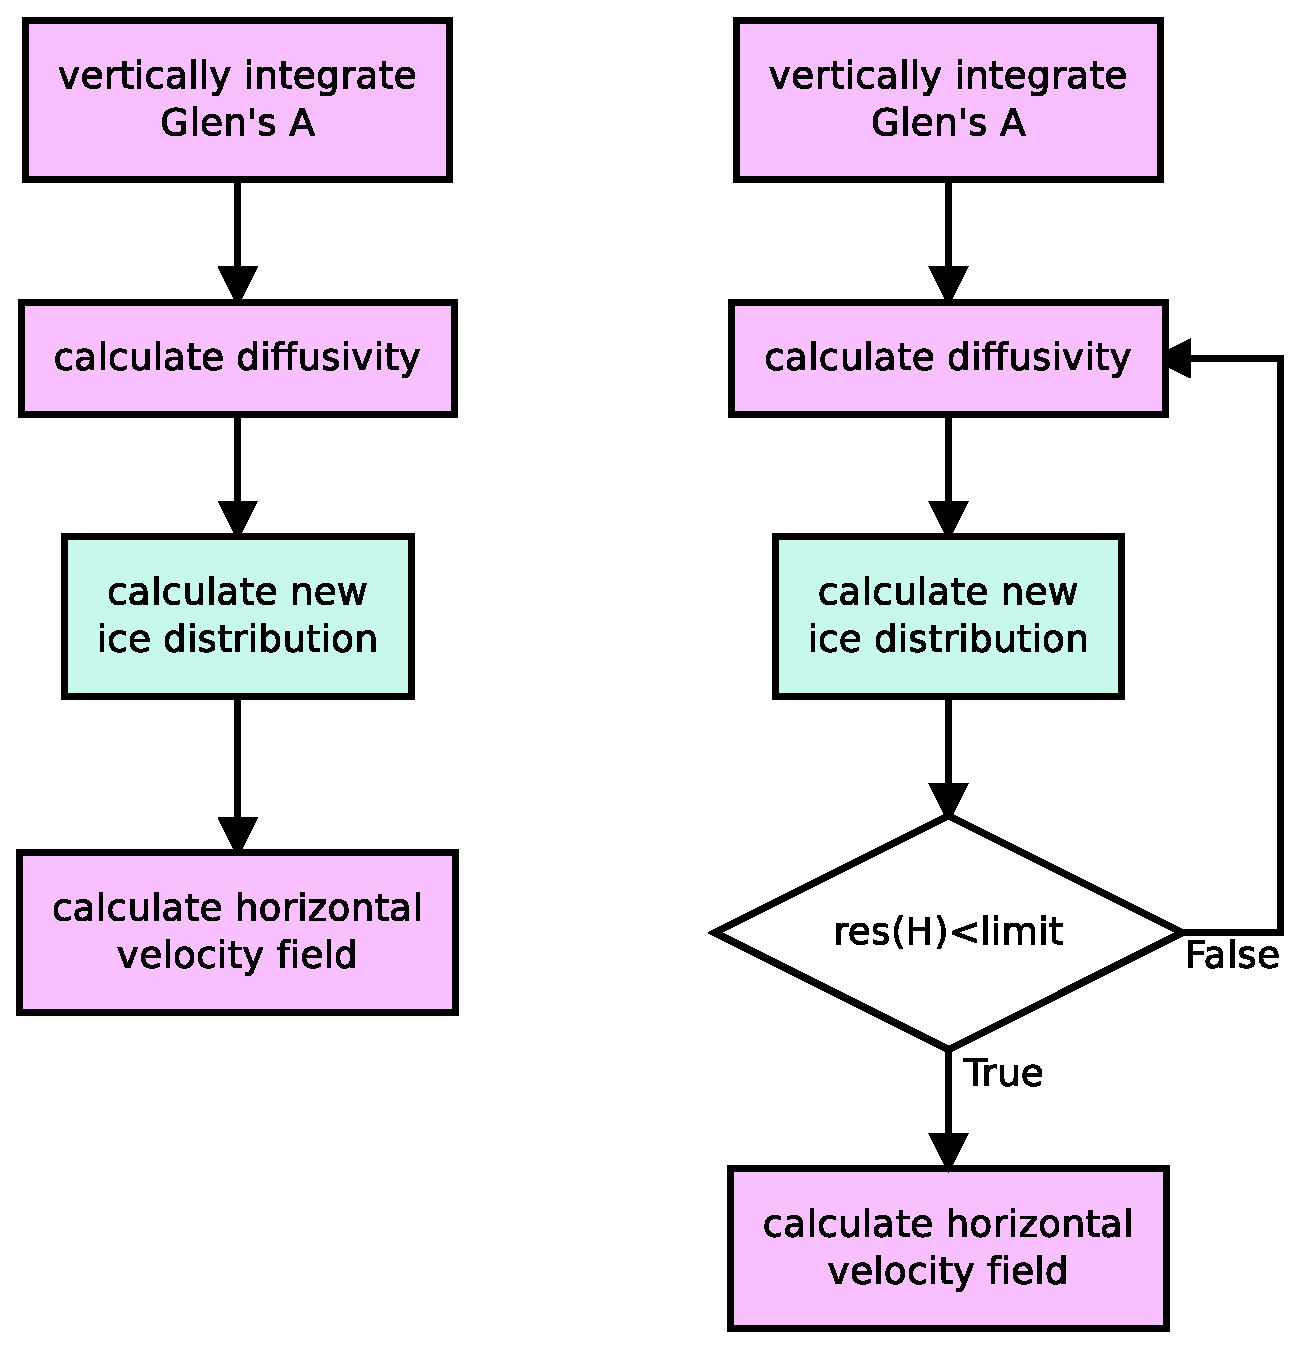
\includegraphics[width=0.5\textwidth]{\dir/figs/thick_evo.eps}
  \caption{Flow diagram showing how the linearised solver (on the left) and the non--linear solver work. The inner, linear iteration is contained within the box labeled ``calculate new ice distribution''.}
  \label{kin.fig.solvers}
\end{figure}

\subsection{Calculating Vertical Velocities}

\subsubsection{Grid Velocity}
The vertical grid moves as a result of using a $\sigma$--coordinate system. The grid velocity is
\begin{equation}
  \label{kin.eq.grid_velo}
  w^{\text{grid}}(\sigma)=\frac{\pd s}{\pd t}+\vec u\cdot\vec\nabla s-\sigma\left(\frac{\pd H}{\pd t}+\vec u\cdot\vec\nabla H\right).
\end{equation}
The numerical implementation of \eqref{kin.eq.grid_velo} is straightforward.

\subsubsection{Vertical Velocity}
The discretized version of the vertical velocity equation \eqref{kin.eq.vert_velo_scaled} is slightly more compilicated because the horizontal velocities are calculated on the $(r,s)$ grid. The vertical velocity at the ice base is $w_{i,j,N}=w^{\text{grid}}_{i,j,N}-M_b{i,j}$, where $M_b{i,j}$ is the basal melt rate. Integrating from the bottom, the vertical velocity is then
\begin{equation}
  \label{kin.eq.wvel_unc}
  \begin{split}
  w_{i,j,k}=-\sum_{\tilde{k}=N-1}^1\left\{\mathcal{H}_{i,j}\left(\frac{u^x_{i,j,k}+u^x_{i,j,k+1}}{2}+\frac{v^y_{i,j,k}+v^y_{i,j,k+1}}{2}\right)(\sigma_{k+1}-\sigma_k)\right. \\
     +(\tilde{u}_{i,j,k+1}-\tilde{u}_{i,j,k})  \left(\tilde{s}^x_{i,j}-\frac12(\sigma_{k+1}+\sigma_k)\tilde{H}^x_{i,j}\right)  \\
     \left.+(\tilde{v}_{i,j,k+1}-\tilde{v}_{i,j,k})  \left(\tilde{s}^y_{i,j}-\frac12(\sigma_{k+1}+\sigma_k)\tilde{H}^y_{i,j}\right)\right\} + w_{i,j,N},
  \end{split}
\end{equation}
with the weighted ice thickness
\begin{equation*}
  \begin{split}
  \mathcal{H}_{i,j}=\frac{4H_{i,j}+2(H_{i-1,j}+H_{i+1,j}+H_{i,j-1}+H_{i,j+1})}{16}\\
  +\frac{H_{i-1,j-1}+H_{i+1,j-1}+H_{i+1,j+1}+H_{i-1,j+1}}{16}.    
  \end{split}
\end{equation*}

This scheme produces vertical velocities at the ice divide which are too small. The vertical velocities on the ice surface are given by the upper kinematic boundary condition \eqref{kin.eq.upper_bc}. Equation \eqref{kin.eq.wvel_unc} can be corrected with
\begin{equation}
  \label{kin.eq.wvel_cor}
   w^\ast_{i,j,k}=w_{i,j,k}-(1-\sigma_k)(w_{i,j,k}-{w_s}_{i,j}),
\end{equation}
where ${w_s}_{i,j}$ is the vertical velocity at the ice surface given by \eqref{kin.eq.upper_bc}. Figure \ref{kin.fig.w_profile} shows the different vertical velocities at the ice surface.
\begin{figure}[htbp]
  \centering
  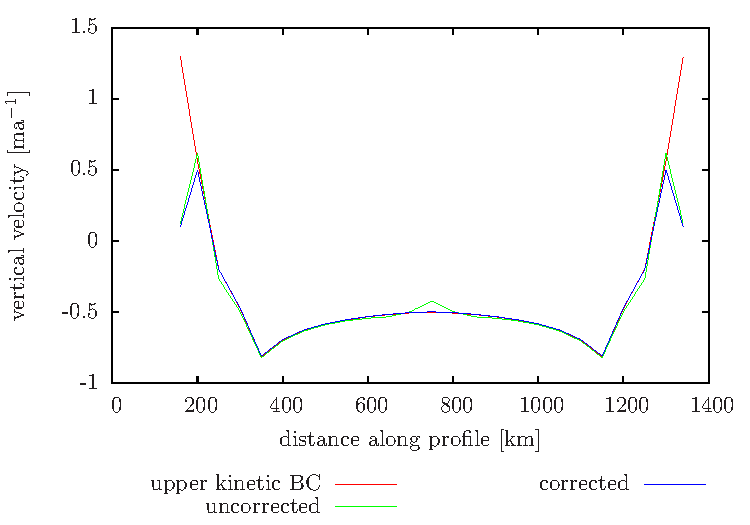
\includegraphics{\dir/gnu/w_profile.eps}
  \caption{Vertical ice surface velocities of the EISMINT-1 moving margin experiment.}
  \label{kin.fig.w_profile}
\end{figure}
The difference between the vertical velocities calculated by the model and the vertical velocities given by \eqref{kin.eq.upper_bc} at the ice margin are due to the fact that temperatures and velocities are only calculated when the ice is thicker than a certain threshold value which is not met at the ice margin.

Figure \ref{kin.fig.wt_sigma} shows vertical profiles of the vertical velocity at the ice divide and a point halfway between the divide and the domain margin. A corresponding temperature profile is also shown since the vertical velocity determines the vertical temperature advection (see Section \ref{temp.sec.vert_ad}).
\begin{figure}[htbp]
  \centering
  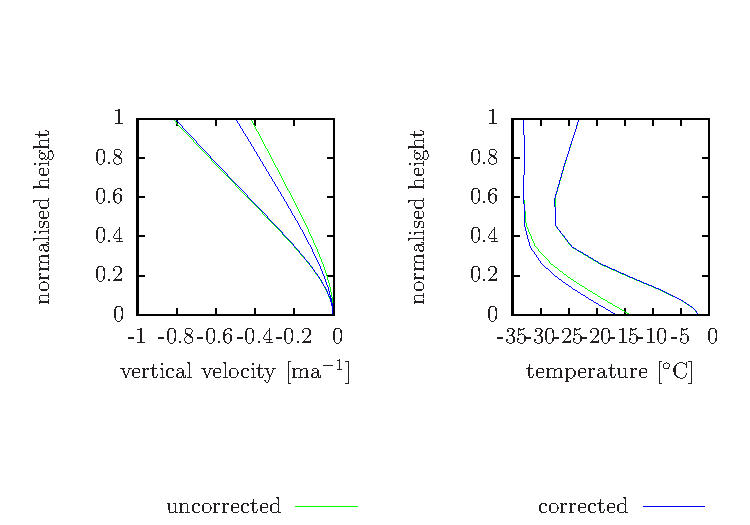
\includegraphics{\dir/gnu/wt_sigma.eps}
  \caption{Vertical velocity and temperature distribution for columns at the ice divide and a point halfway between the divide and the domain margin.}
  \label{kin.fig.wt_sigma}
\end{figure}


\section{Temperature Solver}
The flow law, Equation \eqref{kin.eq.flowlaw}, depends on the temperature of ice. It is, therefore, necessary to determine how the distribution of ice temperatures changes with a changing ice sheet configuration. The thermal evolution of the ice sheet is described by
\begin{equation}
  \label{temp.eq.temp_z}
  \frac{\pd T}{\pd t}=\frac{k}{\rho c}\nabla^2T-\vec{u}\cdot\vec\nabla T+\frac\Phi{\rho c}-w\frac{\pd T}{\pd z},
\end{equation}
where $T$ is the absolute temperature, $k$ is the thermal conductivity of ice, $c$ is the specific heat capacity and $\Phi$ is the heat generated due to internal friction. In the $\sigma$--coordinate system, Equation \eqref{temp.eq.temp_z}, becomes
\begin{equation}
  \label{temp.eq.temp}
  \frac{\pd T}{\pd t} = \frac{k}{\rho cH^2}\frac{\pd^2T}{\pd\sigma^2} - \vec{u}\cdot\vec\nabla T + \frac{\sigma g}c\frac{\pd \vec{u}}{\pd\sigma}\cdot\vec\nabla s + \frac1H\frac{\pd T}{\pd\sigma}\left(w-w_{\text{grid}}\right)
\end{equation}
The terms represents (1) vertical diffusion, (2) horizontal advection, (3) internal heat generation due to friction and (4) vertical advection and a correction due to the sigma coordinate system. Let's rewrite \eqref{temp.eq.temp} to introduce some names:
\begin{equation}
  \label{temp.eq.temp2}
  \frac{\pd T}{\pd t} = a\frac{\pd^2T}{\pd\sigma^2} +b(\sigma) + \Phi(\sigma) + c(\sigma)\frac{\pd T}{\pd\sigma},
\end{equation}
where
\begin{subequations}
  \begin{align}
    a&=\frac{k}{\rho cH^2} \\
    \label{temp.eq.hadv}
    b(\sigma)&=-\vec{u}\cdot\vec\nabla T\\
    \Phi(\sigma)&=\frac{\sigma g}c\frac{\pd \vec{u}}{\pd\sigma}\cdot\vec\nabla s \\
    c(\sigma)&=\frac1H\left(w-w_{\text{grid}}\right)
  \end{align}
\end{subequations}

\subsection{Vertical Diffusion}
Discretisation of $\pd^2T/\pd\sigma^2$ is slightly complicated because the vertical grid is irregular. Using Taylor series the central difference formulas are
\begin{subequations}
  \begin{align}
    \label{temp.eq.d1}
    \left.\frac{\pd T}{\pd\sigma}\right|_{\sigma_{k-1/2}}&=\frac{T_k-T_{k-1}}{\sigma_k-\sigma_{k-1}}\\
    \intertext{and}
    \label{temp.eq.d2}
    \left.\frac{\pd T}{\pd\sigma}\right|_{\sigma_{k+1/2}}&=\frac{T_{k+1}-T_k}{\sigma_{k+1}-\sigma_k}\\
    \intertext{The second partial derivative is then, also using central differences:}
    \label{temp.eq.d3}
    \left.\frac{\pd^2 T}{\pd\sigma^2}\right|_{\sigma_k} &= \frac{\left.{\pd T}/{\pd\sigma}\right|_{\sigma_{k+1/2}} - \left.{\pd T}/{\pd\sigma}\right|_{\sigma_{k-1/2}}}{1/2\left(\sigma_{k+1}-\sigma_{k-1}\right)}\\
    \intertext{Inserting \eqref{temp.eq.d1} and \eqref{temp.eq.d2} into \eqref{temp.eq.d3}, we get:}
    \label{temp.eq.d4}
    &=\frac{2(T_{k+1}-T_k)}{(\sigma_{k+1}-\sigma_k)(\sigma_{k+1}-\sigma_{k-1})}-\frac{2(T_k-T_{k-1})}{(\sigma_k-\sigma_{k-1})(\sigma_{k+1}-\sigma_{k-1})}
  \end{align}
\end{subequations}
Finally, the terms of equation \eqref{temp.eq.d4} are rearranged:
\begin{multline}
  \label{temp.eq.dsigma2}
  \left.\frac{\pd^2 T}{\pd\sigma^2}\right|_{\sigma_k} = \frac{2T_{k-1}}{(\sigma_k-\sigma_{k-1})(\sigma_{k+1}-\sigma_{k-1})} - \frac{2T_k}{(\sigma_{k+1}-\sigma_k)(\sigma_k-\sigma_{k-1})}\\
  + \frac{2T_{k+1}}{(\sigma_{k+1}-\sigma_k)(\sigma_{k+1}-\sigma_{k-1})}
\end{multline}

\subsection{Horizontal Advection}
The horizontal advection term, $- \vec{u}\cdot\vec\nabla T$ is solved using an upwinding scheme. Let's start with the 1--dimensional case. The method discussed can be straightforwadly extented to 2D. As always, the temperature function is expressed as a Taylor series.
\begin{subequations}
  \begin{align}
    \label{temp.eq.taylor1}
    T(x+\Delta x) &=T(x)+\Delta xT'(x)+\frac{\Delta x^2}2T''(x)+\ldots\\
    \intertext{If we subsitute $\Delta x$ with $2\Delta x$, Equation \eqref{temp.eq.taylor1}}
    \label{temp.eq.taylor2}
    T(x+2\Delta x) &=T(x)+2\Delta xT'(x)+2\Delta x^2T''(x)+\ldots
  \end{align}
\end{subequations}
From \eqref{temp.eq.taylor1} and \eqref{temp.eq.taylor2} we can construct a difference formula where the $\mathcal{O}(\Delta x^2)$ error is cancelled, by multiplying \eqref{temp.eq.taylor1} with 4 and substracting the result from \eqref{temp.eq.taylor2}:
\begin{subequations}
  \begin{align}
    \label{temp.eq.forward_h3}
    T_+'(x)&=\frac{4T(x+\Delta x)-T(x+2\Delta x)-3T(x)}{2\Delta x}\\
    \intertext{and similarly for the backward difference:}
    T_-'(x)&=-\frac{4T(x-\Delta x)-T(x-2\Delta x)-3T(x)}{2\Delta x}
    \end{align}
\end{subequations}
So the horizontal advection term in one dimensions becomes:
\begin{equation}
  b_x = -u_x\frac{\pd T}{\pd x}=\frac{-u_x}{2\Delta x}
  \begin{cases}
    -(4T_{i-1}-T_{i-2}-3T_i) & \text{when $u_x>0$} \\
    4T_{i+1}-T_{i+2}-3T_i & \text{when $u_x<0$} \\
  \end{cases}
\end{equation}
A similar expression is found for $b_y$ by simply substituting $y$ for $x$. Finally, the combined horizontal advection term, is simply
\begin{equation}
  b=-\vec{u}\cdot\vec\nabla T=-\left(u_x\frac{\pd T}{\pd x}+u_y\frac{\pd T}{\pd y}\right)=b_x+b_y=b_1+b_2T_i
\end{equation}

\subsection{Heat Generation}
Taking the derivative of \eqref{kin.eq.vert_velo_sigma} with respect to $\sigma$, we get
\begin{equation}
  \frac{\pd u_x}{\pd\sigma} = -2(\rho g)^nH^{n+1}|\vec\nabla s|^{n-1}\frac{\pd s}{\pd x}A(T^\ast)\sigma^n
\end{equation}
Thus,
\begin{equation}
\begin{split}
  \Phi(\sigma) &= \frac{\sigma g}c\frac{\pd \vec{u}}{\pd\sigma}\cdot\vec\nabla s  = \frac{\sigma g}c\left(\frac{\pd u_x}{\pd \sigma}\frac{\pd s}{\pd x} + \frac{\pd u_y}{\pd \sigma}\frac{\pd s}{\pd y}\right)\\
       &= -2(\rho g)^nH^{n+1}|\vec\nabla s|^{n-1}\frac{\sigma g}cA(T^\ast)\sigma^n \left(\left(\frac{\pd s}{\pd x}\right)^2+\left(\frac{\pd s}{\pd y}\right)^2\right) \\
       &= -\frac2{c\rho}(g\sigma\rho)^{n+1}\left(H|\vec\nabla s|\right)^{n+1}A(T^\ast)
\end{split}  
\end{equation}

The constant factor $\frac2{c\rho}(g\sigma\rho)^{n+1}$ is calculated during initialisation in the subroutine \texttt{init\_temp}. This factor is assigned to array \texttt{c1(1:upn)}. \texttt{c1} also includes various scaling factors and the factor $1/16$ to normalise $\mathcal{A}$.

The next factor, $\left(H|\vec\nabla s|\right)^{n+1}$ is calculated in the subroutine \texttt{finddisp}:
\begin{equation}
  {c_2}_{i,j} = \left(\tilde{H}_{i,j}\sqrt{\tilde{S_x}_{i,j}^2+\tilde{S_y}_{i,j}^2}\right)^{n+1},
\end{equation}


The final factor is found by averaging over the neighbouring nodes:
\begin{equation}
  \mathcal{A}_{i,j}=4A_{i,j}+2(A_{i-1,j}+A_{i+1,j}+A_{i,j-1}+A_{i,j+1})+(A_{i-1,j-1}+A_{i+1,j-1}+A_{i+1,j+1}+A_{i-1,j+1})
\end{equation}

\subsection{Vertical Advection}\label{temp.sec.vert_ad}
The vertical advection term, $\pd T/\pd\sigma$ is solved using the central difference formula for unevenly spaced nodes:
\begin{equation}
  \frac{\pd T}{\pd\sigma}=\frac{T_{k+1}-T_{k-1}}{\sigma_{k+1}-\sigma_{k-1}}
\end{equation}

\subsection{Boundary Conditions}
At the upper boundary, ice temperatures are set to the surface temperature, $T_{\text{surf}}$. The ice at the base is heated by the geothermal heat flux and sliding friction:
\begin{equation}
  \left.\frac{\pd T}{\pd\sigma}\right|_{\sigma=1}=-\frac{GH}k-\frac{H\vec{\tau}_b\cdot\vec{u}(1)}k,
\end{equation}
where $\vec{\tau}_b=-\rho gH\vec\nabla s$ is the basal shear stress and $\vec{u}(1)$ is the basal ice velocity. Ice temperatures are held constant if they reach the pressure melting point of ice, i.e.
\begin{equation}
  T^\ast=T_{\text{pmp}} \quad\text{if $T\ge T_{\text{pmp}}$}.
\end{equation}
Excess heat is then used to formulate a melt rate, $S$:
\begin{equation}
  \label{temp.eq.meltrate}
  S=\frac{k}{\rho L}\left(\frac{\pd T^\ast}{\pd z}-\frac{\pd T}{\pd z}\right),
\end{equation}
where $L$ is the specific latent heat of fusion. Finally, basal temperatures are held constant, if the ice is floating:
\begin{equation}
  \frac{\pd T(1)}{\pd t}  = 0.
\end{equation}


\subsection{Putting it all together}
Equation \eqref{temp.eq.temp} is solved for each ice column. The horizontal dependency of the horizontal advection term, \eqref{temp.eq.hadv}, is resolved by iterating the vertical solution. Putting the individual terms together using a fully explicit finite differences scheme, Equation \eqref{temp.eq.temp2} becomes
\begin{subequations}
  \begin{multline}
    \label{temp.eq.temp3a}
    \frac{T_{k,t+1}-T_{k,t}}{\Delta t} = \left(\frac{2aT_{k-1,t}}{(\sigma_k-\sigma_{k-1})(\sigma_{k+1}-\sigma_{k-1})} - \frac{2aT_{k,t}}{(\sigma_{k+1}-\sigma_k)(\sigma_k-\sigma_{k-1,t})}\right. \\
    \left.+ \frac{2aT_{k+1,t}}{(\sigma_{k+1}-\sigma_k)(\sigma_{k+1}-\sigma_{k-1})}\right)+{b_1}_{k,t}+{b_2}_kT_{k,t}+\Phi_k+c_k\frac{T_{k+1,t}-T_{k-1,t}}{\sigma_{k+1}-\sigma_{k-1}}
\end{multline}
and similarly the fully implicit scheme
  \begin{multline}
    \label{temp.eq.temp3b}
    \frac{T_{k,t+1}-T_{k,t}}{\Delta t} = \left(\frac{2aT_{k-1,t+1}}{(\sigma_k-\sigma_{k-1})(\sigma_{k+1}-\sigma_{k-1})} - \frac{2aT_{k,t+1}}{(\sigma_{k+1}-\sigma_k)(\sigma_k-\sigma_{k-1,t+1})}\right. \\
    \left.+ \frac{2aT_{k+1,t+1}}{(\sigma_{k+1}-\sigma_k)(\sigma_{k+1}-\sigma_{k-1})}\right)+{b_1}_{k,t+1}+{b_2}_kT_{k,t+1}+\Phi_k+c_k\frac{T_{k+1,t+1}-T_{k-1,t+1}}{\sigma_{k+1}-\sigma_{k-1}}
\end{multline}
\end{subequations}
Taking the average of Equations \eqref{temp.eq.temp3a} and \eqref{temp.eq.temp3b} gives the \emph{Crank--Nicholson scheme}. The resulting equation is then rearranged and terms of $T_{k-1,t+1}$, $T_{k,t+1}$ and $T_{k+1,t+1}$ are combined to give the tri--diagonal system
\begin{equation}
  \alpha_kT_{k-1,t+1}+\beta_kT_{k,t+1}+\gamma_kT_{k+1,t+1}=\delta_k
\end{equation}
where, for $k=2,N-1$
\begin{subequations}
  \begin{align}
    \alpha_k &= -\frac12\frac{2a\Delta t}{(\sigma_k-\sigma_{k-1})(\sigma_{k+1}-\sigma_{k-1})}+\frac12\frac{c_k\Delta t}{\sigma_{k+1}-\sigma_{k-1}} \\
    \beta_k &= 1+\frac12\frac{2a\Delta t}{(\sigma_{k+1}-\sigma_k)(\sigma_k-\sigma_{k-1})}-\frac12{b_2}_k\Delta t=1-\alpha_k-\gamma_k-\frac12{b_2}_k\Delta t\\
    \gamma_k &= -\frac12\frac{2a\Delta t}{(\sigma_{k+1}-\sigma_k)(\sigma_{k+1}-\sigma_{k-1})}-\frac12\frac{c_k\Delta t}{\sigma_{k+1}-\sigma_{k-1}} \\
    \delta_k &= -\alpha_kT_{k-1,t}+(2-\beta_k)T_{k,t}-\gamma_kT_{k+1,t}+\frac12({b_1}_{k,t}+{b_1}_{k,t+1})\Delta t+\Phi_k\Delta t
  \end{align}

\subsubsection{Boundary Conditions}
At the upper boundary:
\begin{equation}
  \alpha_1=0,\quad\beta_1=1,\quad\gamma_1=0,\quad\delta_1=T_{\text{surf}}
\end{equation}
\end{subequations}


The lower boundary condition is somewhat more complicated. Here we only look at the case when the temperature is below the pressure melting point of ice. BC for floating ice and temperatures at the pressure melting point of ice are trivial. The geothermal heat flux is applied at the lower boundary, i.e. Equation \eqref{temp.eq.d2} becomes
\begin{equation}
  \label{temp.eq.d2-lb}
  \left.\frac{\pd T}{\pd\sigma}\right|_{\sigma_{k+1/2}}=-\frac{GH}k
\end{equation}
Assuming that $\sigma_k-\sigma_{k-1}=\sigma_{k+1}-\sigma_k=\Delta\sigma$ and inserting \eqref{temp.eq.d1} and \eqref{temp.eq.d2-lb} into \eqref{temp.eq.d3}, the second partial derivative becomes
\begin{equation}
  \left.\frac{\pd^2 T}{\pd\sigma^2}\right|_{\sigma_N} = \left(-\frac{GH}k-\frac{T_N-T_{N-1}}{\Delta\sigma}\right)/\Delta\sigma=-\frac{GH}{k\Delta\sigma}-\frac{T_N-T_{N-1}}{\Delta\sigma^2}
\end{equation}
Inserting the new conduction term and replacing the derivative of the vertical advection term with the Neumann boundary condition, Equation \eqref{temp.eq.temp3a} becomes
\begin{subequations}
  \begin{equation}
    \frac{T_{N,t+1}-T_{N,t}}{\Delta t} = -a\left(\frac{GH}{k\Delta\sigma}+\frac{T_{N,t}-T_{N-1,t}}{\Delta\sigma^2}\right)+{b_1}_{N,t}+{b_2}_NT_{N,t}+\Phi_N-c_N\frac{GH}k
  \end{equation}
  and similarly for Equation \eqref{temp.eq.temp3b}
  \begin{multline}
    \frac{T_{N,t+1}-T_{N,t}}{\Delta t} = -a\left(\frac{GH}{k\Delta\sigma}+\frac{T_{N,t+1}-T_{N-1,t+1}}{\Delta\sigma^2}\right)+{b_1}_{N,t+1}+{b_2}_NT_{N,t+1}\\
    +\Phi_N-c_N\frac{GH}k
  \end{multline}
\end{subequations}
The elements of the tri--diagonal system at the lower boundary are then
\begin{subequations}
  \begin{gather}
    \alpha_N =-\frac{a\Delta t}{2(\sigma_N-\sigma_{N-1})^2}\\
    \beta_N = 1-\alpha_N+\frac12{b_2}_N\Delta t\\
    \gamma_N = 0 \\
    \begin{split}
      \delta_N =&-\alpha_NT_{N-1,t}+(2-\beta_N)T_{N,t}-a\frac{GH\Delta t}{k(\sigma_N-\sigma_{N-1})}\\
      &+\frac12({b_1}_{N,t}+{b_1}_{N,t+1})\Delta t+\Phi_N\Delta t-c_N\frac{GH\Delta t}k
    \end{split}
  \end{gather}
\end{subequations}


\section{Basal Boundary Condition}
This section describes the formulation of the basal boundary condition.
An interface for the upper boundary condition (atmospheric BC) is easily defined by the surface temperature and mass balance. Similarly, the basal boundary consists of mechanical and thermal boundary conditions. The complications arise because the thermal and mechanical boundary conditions depend on each other. The interface of the basal boundary can be described with the following fields (see also Fig. \ref{num.fig.basal_bc}):
\begin{enumerate}
\item \textbf{basal traction:} This field specifies a parameter which is used to allow basal sliding.
\item \textbf{basal heat flux:} This is the heat flux entering the ice sheet from below.
\item \textbf{basal water depth:} The presence of basal melt water affects the basal ice temperature.
\end{enumerate}
Also, the ice sheet model calculates a melt/freeze rate based on the temperature gradient and basal water depth. This is handled by Glide.

\begin{figure}[htbp]
  \centering
  
\includegraphics[width=0.9\textwidth]{\dir/figs/basal_bc.eps}
  \caption{Basal boundary condition.}
  \label{num.fig.basal_bc}
\end{figure}

\subsection{Mechanical boundary conditions}
If the ice is not frozen to the bed, basal d\'{e}collement may occur. This can be parameterized by a traction factor, $t_b$. 
Within the ice sheet model, $t_b$ can be used to calculate basal sliding velocities $\vec{u}_b$ in the case of zero--order physics. That is,
\begin{equation}
  \vec{u}_b=t_b\vec{\tau}_b,
\end{equation}
where $\tau_b$ is the basal shear stress. Alternatively, $t_b$ can be used as part of the stress--balance calculations when the model is used with higher order physics. In simple models $t_b$ may be uniform or prescribed as a spatial variable. More complex models may wish to make $t_b$ dependent on other variables, such as basal melt rate. Typically $t_b$ will depend on the presence of basal water.

The second mechanical boundary condition, basal melting/freeze--on $M_b$, is handled within the ice sheet model. The details are described in Section \ref{num.sec.bc_melt}.

\subsection{Thermal boundary conditions}
The thermal boundary condition at the ice base is more complicated than the mechanical BC. The ice is heated from below by the geothermal heat flux. Heat is generated by friction with the bed. Furthermore, the ice temperature is constrained to be less than or equal to the pressure melting point of ice. The thermal boundary condition is a flux condition if there is no water present. If there is water, the basal temperature is set to the pressure melting temperature. (If it were lower, there would be no water, and if it were higher, there would be no ice.)

\subsubsection{Basal melting and freezing}\label{num.sec.bc_melt}
At the ice base, $z=b$, we can define outgoing and incoming heat fluxes, $H_o$ and $H_i$:
\begin{subequations}
  \begin{align}
    H_o&=-k_{\text{ice}}\left.\frac{\pd T}{\pd z}\right|_{z=b^+}\\
    \intertext{and}
    H_i&=-k_{\text{rock}}\left.\frac{\pd T}{\pd z}\right|_{z=b^-}+\vec{u}_b\cdot\vec{\tau}_b+
    \begin{cases}
      {\rho_{\text{ice}}M_b}/{L} & \text{when $M_b<0$} \\
      0 & \text{otherwise}
    \end{cases}
  \end{align}
\end{subequations}
where $k_{\text{ice}}$ and $k_{\text{rock}}$ are the thermal conductivities of ice and rock, $\vec{u}_b\cdot\vec{\tau}_b$ is the heat generated by friction with the bed, and $L$ is the latent heat of fusion. The basal melt/freeze--on rate $M_b$ can then be calculated from the difference between the incoming and outgoing heat fluxes:
\begin{equation}
  \label{bc.eq.meltrate}
  M_b=\frac{H_i-H_o}{\rho_{\text{ice}}L}
\end{equation}
There is freeze--on if $M_b < 0$, and basal melting if $B_b > 0$.

\subsubsection{Geothermal Heat Flux}
The heat flux accross the basal boundary depends on past temperature variations since temperature perturbations penetrate the bed rock if the ice is frozen to the ground \citep{Ritz1987}. 
The heat equation for the bed rock layer is given by the diffusion equation
\begin{equation}
  \label{num.eq.diffu_rock}
  \frac{\pd T}{\pd t} = \frac{k_{\text{rock}}}{\rho_{\text{rock}}c_{\text{rock}}}\nabla^2T=\frac{k_{\text{rock}}}{\rho_{\text{rock}}c_{\text{rock}}} 
  \left(\frac{\pd^2 T}{\pd x^2}+\frac{\pd^2 T}{\pd y^2}+\frac{\pd^2 T}{\pd z^2}\right),
\end{equation}
where $k_{\text{rock}}$ is the thermal conductivity, $\rho_{\text{rock}}$ the density and $c_{\text{rock}}$ the specific heat capacity of the bed rock layer. 

Initial conditions for the temperature field $T$ are found by applying the geothermal heat flux, $G$ to an arbitrary surface temperature $T_0$:
\begin{equation}
  T(x,y,z)=T_0+\frac{G}{k_{\text{rock}}}z.
\end{equation}
This ensures that initially the geothermal heat flux experienced by the ice sheet is equal to the regional heat flux. The basal boundary condition of the bedrock layer is kept constant, i.e.
\begin{equation}
  T(x,y,H_{\text{rock}})=T_0+\frac{G}{k_{\text{rock}}}H_{\text{rock}}.
\end{equation}
Lateral boundary conditions are given by
\begin{equation}
  \left.\frac{\pd T}{\pd x}\right|_{x=0} = \left.\frac{\pd T}{\pd x}\right|_{x=L_x} = \left.\frac{\pd T}{\pd y}\right|_{y=0} = \left.\frac{\pd T}{\pd y}\right|_{y=L_y} = 0.
\end{equation}
At the upper boundary, the heat flux of the rock layer has to be matched with the heat flux in the basal ice layer when the ice is frozen to the bed, i.e.
\begin{equation}
  \label{num.eq.gthf_bc}
  k_{\text{rock}}\left.\frac{\pd T}{\pd z}\right|_{z=-0}=k_{\text{ice}}\left.\frac{\pd T}{\pd z}\right|_{z=+0}.
\end{equation}
Otherwise the temperature of the top bedrock layer is set to the surface temperature (if the cell has been occupied by ice, but there is no ice present) or the basal ice temperature (if there is ice). Equation \eqref{num.eq.gthf_bc} is automatically fulfilled if we set the top bedrock temperature to the basal ice temperature \emph{everywhere} and then calculate the geothermal heat flux to be used as boundary condition for Equation \eqref{temp.eq.temp_z}.



\subsection{Numerical Solution}
The horizontal grid is described in Section \ref{num.sec.grid}. The vertical grid is irregular like the vertical grid of the ice sheet model. However, it is not scaled. Also for now, I have ignored topography or isostatic adjustment, i.e. the bedrock layer is assumed to be flat and constant.

The horizontal second derivative in Equation \eqref{num.eq.diffu_rock} becomes using finite--differences
\begin{equation}
  \left.\frac{\pd^2T}{\pd x^2}\right|_{x_i,y_i,z_i} = T_{xx,i,j,k} = \frac{T_{i+1,j,k}-2T_{i,j,k}+T_{i-1,j,k}}{\Delta x}
\end{equation}
and similarly for $\pd^2T/\pd y^2$. The vertical second derivative $\pd^2T/\pd z^2$ is similar to Equation \eqref{temp.eq.dsigma2}:
\begin{multline}
  \left.\frac{\pd^2 T}{\pd z^2}\right|_{x_i,y_i,z_i} = T_{zz,i,j,k} = \frac{2T_{i,j,k-1}}{(z_k-z_{k-1})(z_{k+1}-z_{k-1})} - \frac{2T_{i,j,k}}{(z_{k+1}-z_k)(z_k-z_{k-1})}\\
  + \frac{2T_{i,j,k+1}}{(z_{k+1}-z_k)(z_{k+1}-z_{k-1})}
\end{multline}


Using the Crank-Nicholson scheme, Equation \eqref{num.eq.diffu_rock} becomes
\begin{equation}
  \label{num.eq.diffu_rock_disc}
  \frac{T_{i,j,k}^{t+1}-T_{i,j,k}^{t}}{\Delta t}=D\left\{\frac{T_{xx,i,j,k}^{t+1}+T_{xx,i,j,k}^{t}}2 + \frac{T_{yy,i,j,k}^{t+1}+T_{yy,i,j,k}^{t}}2 + \frac{T_{zz,i,j,k}^{t+1}+T_{zz,i,j,k}^{t}}2 \right\},
\end{equation}
with $D=k_{\text{rock}}/(\rho_{\text{rock}}c_{\text{rock}})$. Equation \eqref{num.eq.diffu_rock_disc} is solved by gathering all $T^{t+1}$ terms on the LHS and all other terms on the RHS. The index $(i,j,k)$ is linearised using $\iota = i+(j-1)N+(k-1)NM$. The resulting matrix system is solved using the same bi--conjugate gradient solver as for the ice thickness evolution.



\subsection{Basal hydrology}
It is clear from the discussion above that the presence of basal water plays a crucial role in specifying both the mechanical and thermal boundary conditions. However, the treatment of basal water can vary greatly. Basal water is, therefore, left as an unspecified interface. Glide does provide a simple local water balance model which can be run in the absence of more complex models.

\subsection{Putting it all together}
The basal boundary consists of the individual components described in the previous sections. All components are tightly linked with each other. Figure \ref{num.fig.bc_flow} illustrates how the modules are linked and in what order they are resolved.
\begin{figure}[htbp]
  \centering
  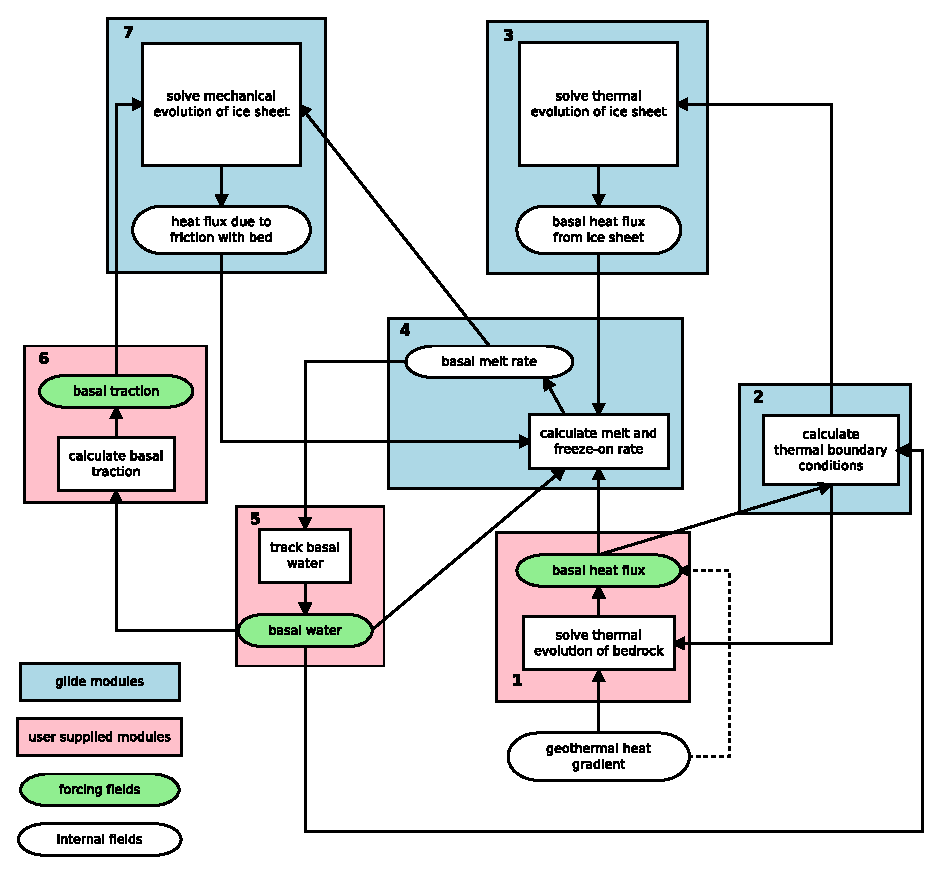
\includegraphics[width=\textwidth]{\dir/figs/basal_alg.eps}
  \caption{Flow diagram illustrating how the various modules communicate with each other by exchanging data fields.}
  \label{num.fig.bc_flow}
\end{figure}
The order of executions is then:
\begin{enumerate}
\item Find the basal heat flux by either solving the equation describing the thermal evolution of the lithosphere, \eqref{num.eq.diffu_rock}, or by using the geothermal heat flux directly. The upper boundary condition of \eqref{num.eq.diffu_rock} is the same as the lower boundary condition of the thermal evolution of the ice sheet.
\item Either (1) the lower boundary condition for the thermal evolution of the ice sheet is given by the basal heat flux from \emph{Step 1}; or (2) if melt water is present, the basal temperature is set to the pressure melting point of ice.
\item Calculate the temperature distribution within the ice sheet given the boundary condition found during \emph{Step 2} and the atmospheric BC.
\item Calculate a melt/freeze--on rate using Equation \eqref{bc.eq.meltrate} given the outgoing heat flux calculated during \emph{Step 3}, friction with the bed (calculated during the previous \emph{Step 7}) and the incoming heat flux from \emph{Step 1}. Freezing occurs only when there is basal water.
\item Track basal water. This is a user supplied module which can take any complexity. Inputs will typically be the melt/freeze--on rate determined during \emph{Step 4}.
\item Calculate the basal traction parameter. Again, this is a user supplied module which typically will involve the presence of basal water (calculated during \emph{Step 5}).
\item Solve the mechanical ice equations given basal traction parameter from \emph{Step 6}.
\end{enumerate}
Clearly, this scheme has the problem that heat is lost if the basal heat flux is such that more water could be frozen than is available. This might be avoided by iterating the process. On the other hand, the heat loss may be negligible if time steps are fairly small.

\section{Isostatic Adjustment}
The ice sheet model includes simple approximations for calculating isostatic adjustment. These approximations depend on how the lithosphere and the mantle are treated. For each subsystem there are two models. The lithosphere can be described as a
\begin{description}
\item[\textbf{local lithosphere:}] the flexural rigidity of the lithosphere is ignored, i.e. this is equivalent to ice floating directly on the asthenosphere;
\item[\textbf{elastic lithosphere:}] the flexural rigidity is taken into account;
\end{description}
while the mantle is treated as a
\begin{description}
\item [\textbf{fluid mantle:}] the mantle behaves like a non-viscous fluid, isostatic equilibrium is reached instantaneously;
\item [\textbf{relaxing mantle:}] the flow within the mantle is approximated by an exponentially decaying hydrostatic response function, i.e. the mantle is treated as a viscous half space.
\end{description}

\subsection{Calculation of ice-water load}
At each isostasy time-step, the load of ice and water is calculated, as an
equivalent mantle-depth ($L$). If the basal elevation is above sea-level, then the
load is simply due to the ice:
\begin{equation}
L=\frac{\rho_i}{\rho_m}H,
\label{load_land_ice}
\end{equation}
where $H$ is the ice thickness, with $\rho_i$ and $\rho_m$ being the densities
of the ice and mantle respectively. In the case where the bedrock is below
sea-level, the load is calculated is that due to a change in sea-level rise and/or
the presence of non-floating ice. When the ice is floating ($\rho_i
H<\rho_o(z_0-h)$), the load is only due to sea-level changes
\begin{equation}
L=\frac{\rho_o}{\rho_m}z_0,
\label{load_sea_float}
\end{equation}
whereas when the ice is grounded, it displaces the water, and adds an
additional load:
\begin{equation}
L=\frac{\rho_i H+\rho_o b_r}{\rho_m}.
\label{load_sea_grounded}
\end{equation}
here, $\rho_o$ is the density of sea water, $z_0$ is the change in sea-level
relative to a reference level and $b_r$ is the bedrock elevation relative to the
same reference level. The value of $b_r$ will be negative for submerged bedrock,
hence the plus sign in (\ref{load_sea_grounded}).

\subsection{Elastic lithosphere model}
This is model is selected by setting \texttt{lithosphere = 1} in the
configuration file. By simulatuing the deformation of the lithosphere, the
deformation seen by the aesthenosphere beneath is calculated. In the absence of this
model, the deformation is that due to Archimedes' Principle, as though the
load were floating on the aesthenosphere.

The elastic lithosphere model is based on work by \cite{Lambeck1980}, and its
implementation is fully described in \cite{Hagdorn2003}. The lithosphere
model only affects the geometry of the deformation --- the timescale for
isostatic adjustment is controlled by the aesthenosphere model. 

The load due to a single (rectangular) grid point is approximated as being
applied to a disc of the same area. The deformation due to a disc of ice of
radius $A$ and thickness $H$ is given by these expressions. For $r<A$:
\begin{equation} 
w(r)=\frac{\rho_i H}{\rho_m}\left[1+C_1\,\mathrm{Ber}\left(\frac{r}{L_r}\right)+C_2\,\mathrm{Bei}\left(\frac{r}{L_r}\right)\right],
\end{equation}
and for $r\geq A$:
\begin{equation}
w(r)=\frac{\rho_i
  H}{\rho_m}\left[D_1\,\mathrm{Ber}\left(\frac{r}{L_r}\right)+D_2\,\mathrm{Bei}\left(\frac{r}{L_r}\right)
+D_3\,\mathrm{Ker}\left(\frac{r}{L_r}\right)+D_4\,\mathrm{Kei}\left(\frac{r}{L_r}\right)\right],
\end{equation}
where $\mathrm{Ber}(x)$, $\mathrm{Bei}(x)$, $\mathrm{Ker}(x)$ and
$\mathrm{Kei}(x)$ are Kelvin functions of zero order, $L_r=(D/\rho_m
g))^{1/4}$ is the radius of relative stiffness, and $D$ is the flexural
rigidity. The constants $C_i$ and $D_i$ are given by
\begin{equation}
\begin{array}{rcl}
C_1&=&a\,\mathrm{Ker}'(a)\\
C_2&=&-a\,\mathrm{Ker}'(a)\\
D_1&=&0\\
D_2&=&0\\
D_3&=&a\,\mathrm{Ber}'(a)\\
D_4&=&-a\,\mathrm{Ber}'(a).
\end{array}
\end{equation}
Here, the prime indicates the first spatial derivative of the Kelvin functions.

\subsection{Relaxing aesthenosphere model}
If a fluid mantle is selected, it adjusts instantly to changes in lithospheric
loading. However, a relaxing mantle is also available.

%%% Local Variables: 
%%% mode: latex
%%% TeX-master: "isos"
%%% End: 



\chapter{Developer Guide}
\renewcommand{\dir}{dg}
\newcommand{\dir}{dg}

\pagestyle{myheadings}
\markright{GLIMMER {\glimmerver} --- Developer's Guide}

\begin{document}
\title{GLIMMER {\glimmerver} --- Developer's Guide}
\author{Magnus Hagdorn\thanks{Magnus.Hagdorn@ed.ac.uk} \and Ian Rutt\thanks{I.C.Rutt@bristol.ac.uk}}
\maketitle
\tableofcontents
\newpage

\newcommand{\dir}{dg}

\pagestyle{myheadings}
\markright{GLIMMER {\glimmerver} --- Developer's Guide}

\begin{document}
\title{GLIMMER {\glimmerver} --- Developer's Guide}
\author{Magnus Hagdorn\thanks{Magnus.Hagdorn@ed.ac.uk} \and Ian Rutt\thanks{I.C.Rutt@bristol.ac.uk}}
\maketitle
\tableofcontents
\newpage

\newcommand{\dir}{dg}

\pagestyle{myheadings}
\markright{GLIMMER {\glimmerver} --- Developer's Guide}

\begin{document}
\title{GLIMMER {\glimmerver} --- Developer's Guide}
\author{Magnus Hagdorn\thanks{Magnus.Hagdorn@ed.ac.uk} \and Ian Rutt\thanks{I.C.Rutt@bristol.ac.uk}}
\maketitle
\tableofcontents
\newpage

\input{\dir/dg.tex}
\end{document}

\end{document}

\end{document}


\renewcommand{\dir}{ext}
\newcommand{\dir}{ext}

\pagestyle{myheadings}

\markright{Glimmer-CISM {\glimmerver} Extension documentation}

\begin{document}
\title{Glimmer-CISM {\glimmerver} Extension Documentation}
\author{Magnus Hagdorn\thanks{Magnus.Hagdorn@ed.ac.uk}, Ian
Rutt\thanks{I.C.Rutt@bristol.ac.uk} \and Tony Payne\thanks{a.j.payne@bristol.ac.uk}}

\maketitle
\tableofcontents
\newpage

\newcommand{\dir}{ext}

\pagestyle{myheadings}

\markright{Glimmer-CISM {\glimmerver} Extension documentation}

\begin{document}
\title{Glimmer-CISM {\glimmerver} Extension Documentation}
\author{Magnus Hagdorn\thanks{Magnus.Hagdorn@ed.ac.uk}, Ian
Rutt\thanks{I.C.Rutt@bristol.ac.uk} \and Tony Payne\thanks{a.j.payne@bristol.ac.uk}}

\maketitle
\tableofcontents
\newpage

\newcommand{\dir}{ext}

\pagestyle{myheadings}

\markright{Glimmer-CISM {\glimmerver} Extension documentation}

\begin{document}
\title{Glimmer-CISM {\glimmerver} Extension Documentation}
\author{Magnus Hagdorn\thanks{Magnus.Hagdorn@ed.ac.uk}, Ian
Rutt\thanks{I.C.Rutt@bristol.ac.uk} \and Tony Payne\thanks{a.j.payne@bristol.ac.uk}}

\maketitle
\tableofcontents
\newpage

\input{\dir/ext.tex}
\bibliography{glimmer}
\end{document}

\bibliography{glimmer}
\end{document}

\bibliography{glimmer}
\end{document}


\part{Appendix}
\appendix
\renewcommand{\dir}{ug}
\chapter{netCDF Variables}
\label{ug.sec.varlist}
The following list shows all the variable names used by GLIMMER. Only variables marked with $^\ast$ are loaded by the input routines.
\section{Glide Variables}
\input{\dir/glide_varlist.tex}
\section{EIS Variables}
\input{\dir/eis_varlist.tex}
\section{GLINT Variables}
\input{\dir/glint_varlist.tex}

\chapter{The GLIMMER API}
\section{GLUM}
GLUM provides some utility subroutines which are shared by all components of GLIMMER.

\subsection{Subroutine \texttt{open\_log}}
\paragraph{Purpose} open and initialise log file

\paragraph{Name and mandatory arguments}
\begin{verbatim}
subroutine open_log
\end{verbatim}

\paragraph{Arguments}
\begin{center}
  \tablefirsthead{%
    \hline
  }
  \tablehead{%
    \hline
    \multicolumn{4}{|p{\textwidth}|}{\emph{\small continued from previous page}}\\
    \hline
  }
  \tabletail{%
    \hline
    \multicolumn{4}{|r|}{\emph{\small continued on next page}}\\
    \hline}
  \tablelasttail{\hline}
  \begin{supertabular*}{\textwidth}{@{\extracolsep{\fill}}lllp{5.5cm}}
    \multicolumn{4}{|l|}{{\bf Mandatory}}\\
    \hline
    \hline
    \multicolumn{4}{|l|}{{\bf Optional}}\\
    \hline
    \texttt{unit} & \texttt{integer} & \texttt{intent(in)} & file unit to use (defualt: 6) \\
    \texttt{fname}& \texttt{character(len=*)} & \texttt{intent(in)} & name of log file (default: \texttt{glide.log})\\ 
  \end{supertabular*}
\end{center}
%%%%%%%%%%%%%%%%%%%%%%%%%%%%%%%%%%%%%%%%%%%%%%%%%%%
\subsection{Subroutine \texttt{ConfigRead}}
\paragraph{Purpose} Read configuration file and store config options.

\paragraph{Name and mandatory arguments}
\begin{verbatim}
subroutine ConfigRead(fname,config)
\end{verbatim}

\paragraph{Arguments}
\begin{center}
  \tablefirsthead{%
    \hline
  }
  \tablehead{%
    \hline
    \multicolumn{4}{|p{\textwidth}|}{\emph{\small continued from previous page}}\\
    \hline
  }
  \tabletail{%
    \hline
    \multicolumn{4}{|r|}{\emph{\small continued on next page}}\\
    \hline}
  \tablelasttail{\hline}
  \begin{supertabular*}{\textwidth}{@{\extracolsep{\fill}}lllp{5.5cm}}
    \multicolumn{4}{|l|}{{\bf Mandatory}}\\
    \hline
    %%
    \texttt{fname} & \texttt{character(len=*)} & \texttt{intent(in)} & name of configuration file to be read\\
    \texttt{config} & \texttt{type(ConfigSection), pointer} & & pointer to first element of linked list containing configuration\\    
  \end{supertabular*}
\end{center}
\paragraph{Additional Notes}
Each section within the configuration file is stored as an element of a linked list. These elements contain another linked list storing the key--value pairs.

%%%%%%%%%%%%%%%%%%%%%%%%%%%%%%%%%%%%%%%%%%%%%%%%%%%
\subsection{Subroutine \texttt{CheckSections}}
\paragraph{Purpose} To check if all sections within a configuration file were subsequently used. Report unused sections to the log.

\paragraph{Name and mandatory arguments}
\begin{verbatim}
subroutine CheckSections(config)
\end{verbatim}
\paragraph{Arguments}
\begin{center}
  \tablefirsthead{%
    \hline
  }
  \tablehead{%
    \hline
    \multicolumn{4}{|p{\textwidth}|}{\emph{\small continued from previous page}}\\
    \hline
  }
  \tabletail{%
    \hline
    \multicolumn{4}{|r|}{\emph{\small continued on next page}}\\
    \hline}
  \tablelasttail{\hline}
  \begin{supertabular*}{\textwidth}{@{\extracolsep{\fill}}lllp{5.5cm}}
    \multicolumn{4}{|l|}{{\bf Mandatory}}\\
    \hline
    %%
    \texttt{config} & \texttt{type(ConfigSection), pointer} & & pointer to first element of linked list containing configuration\\ 
  \end{supertabular*}
\end{center}

%%%%%%%%%%%%%%%%%%%%%%%%%%%%%%%%%%%%%%%%%%%%%%%%%%%
%\subsection{Subroutine \texttt{}}
%\paragraph{Purpose} 
%\paragraph{Name and mandatory arguments}
%\begin{verbatim}
%
%\end{verbatim}
%\paragraph{Arguments}
%\begin{center}
%  \tablefirsthead{%
%    \hline
%  }
%  \tablehead{%
%    \hline
%    \multicolumn{4}{|p{\textwidth}|}{\emph{\small continued from previous page}}\\
%    \hline
%  }
%  \tabletail{%
%    \hline
%    \multicolumn{4}{|r|}{\emph{\small continued on next page}}\\
%    \hline}
%  \tablelasttail{\hline}
%  \begin{supertabular*}{\textwidth}{@{\extracolsep{\fill}}lllp{5.5cm}}
%    \multicolumn{4}{|l|}{{\bf Mandatory}}\\
%    \hline
%    %%
%    \hline
%    \multicolumn{4}{|l|}{{\bf Optional}}\\
%    \hline
%    %%
%  \end{supertabular*}
%\end{center}


\section{GLIDE}\label{ug.sec.glide_api}
%%%%%%%%%%%%%%%%%%%%%%%%%%%%%%%%%%%%%%%%%%%%%%%%%%
\subsection{Subroutine \texttt{glide\_config}}
\paragraph{Purpose} To parse configuration file and print configuration to log
\paragraph{Name and mandatory arguments}
\begin{verbatim}
subroutine glide_config(model,config)
\end{verbatim}
\paragraph{Arguments}
\begin{center}
  \tablefirsthead{%
    \hline
  }
  \tablehead{%
    \hline
    \multicolumn{4}{|p{\textwidth}|}{\emph{\small continued from previous page}}\\
    \hline
  }
  \tabletail{%
    \hline
    \multicolumn{4}{|r|}{\emph{\small continued on next page}}\\
    \hline}
  \tablelasttail{\hline}
  \begin{supertabular*}{\textwidth}{@{\extracolsep{\fill}}lllp{5.5cm}}
    \multicolumn{4}{|l|}{{\bf Mandatory}}\\
    \hline
    %%
    \texttt{model} & \texttt{type(glide\_global\_type)} &\texttt{intent(inout)}& f95 type containing all variables associated with an instance of the model.\\
    \texttt{config} & \texttt{type(ConfigSection), pointer} & & pointer to first element of linked list containing configuration\\ 
  \end{supertabular*}
\end{center}

%%%%%%%%%%%%%%%%%%%%%%%%%%%%%%%%%%%%%%%%%%%%%%%%%%
\subsection{Subroutine \texttt{glide\_initialise}}
\paragraph{Purpose} To initialise the basic ice sheet model
\paragraph{Name and mandatory arguments}
\begin{verbatim}
subroutine glide_initialise(model)
\end{verbatim}
\paragraph{Arguments}
\begin{center}
  \tablefirsthead{%
    \hline
  }
  \tablehead{%
    \hline
    \multicolumn{4}{|p{\textwidth}|}{\emph{\small continued from previous page}}\\
    \hline
  }
  \tabletail{%
    \hline
    \multicolumn{4}{|r|}{\emph{\small continued on next page}}\\
    \hline}
  \tablelasttail{\hline}
  \begin{supertabular*}{\textwidth}{@{\extracolsep{\fill}}lllp{5.5cm}}
    \multicolumn{4}{|l|}{{\bf Mandatory}}\\
    \hline
    %%
    \texttt{model} & \texttt{type(glide\_global\_type)} &\texttt{intent(inout)}& f95 type containing all variables associated with an instance of the model.\\
  \end{supertabular*}
\end{center}
\paragraph{Additional Notes}
This subroutine initialises the model. Memory for all variables is allocated. Input files are opend and read. Output files are created. Variables are scaled.

%%%%%%%%%%%%%%%%%%%%%%%%%%%%%%%%%%%%%%%%%%%%%%%%%%%
\subsection{Subroutine \texttt{glide\_nc\_fillall}}
\paragraph{Purpose} fill netCDF coordinate variables.
\paragraph{Name and mandatory arguments}
\begin{verbatim}
subroutine glide_nc_fillall(model)
\end{verbatim}
\paragraph{Arguments}
\begin{center}
  \tablefirsthead{%
    \hline
  }
  \tablehead{%
    \hline
    \multicolumn{4}{|p{\textwidth}|}{\emph{\small continued from previous page}}\\
    \hline
  }
  \tabletail{%
    \hline
    \multicolumn{4}{|r|}{\emph{\small continued on next page}}\\
    \hline}
  \tablelasttail{\hline}
  \begin{supertabular*}{\textwidth}{@{\extracolsep{\fill}}lllp{5.5cm}}
    \multicolumn{4}{|l|}{{\bf Mandatory}}\\
    \hline
    %%
    \texttt{model} & \texttt{type(glide\_global\_type)} &\texttt{intent(inout)}& f95 type containing all variables associated with an instance of the model.\\
  \end{supertabular*}
\end{center}

%%%%%%%%%%%%%%%%%%%%%%%%%%%%%%%%%%%%%%%%%%%%%%%%%%%
\subsection{Subroutine \texttt{glide\_tstep\_p1}}
\paragraph{Purpose} Performs first part of time-step of an ice model instance: calculate vertical velocity and temperature field. Set model time.
\paragraph{Name and mandatory arguments}
\begin{verbatim}
subroutine glide_tstep_p1(model,time)
\end{verbatim}
\paragraph{Arguments}
\begin{center}
  \tablefirsthead{%
    \hline
  }
  \tablehead{%
    \hline
    \multicolumn{4}{|p{\textwidth}|}{\emph{\small continued from previous page}}\\
    \hline
  }
  \tabletail{%
    \hline
    \multicolumn{4}{|r|}{\emph{\small continued on next page}}\\
    \hline}
  \tablelasttail{\hline}
  \begin{supertabular*}{\textwidth}{@{\extracolsep{\fill}}lllp{5.5cm}}
    \multicolumn{4}{|l|}{{\bf Mandatory}}\\
    \hline
    %%
    \texttt{model} & \texttt{type(glide\_global\_type)} &\texttt{intent(inout)}& f95 type containing all variables associated with an instance of the model.\\
    \texttt{time}  & \texttt{real(rk)} & \texttt{intent(in)} & Current time in years\\
  \end{supertabular*}
\end{center}


%%%%%%%%%%%%%%%%%%%%%%%%%%%%%%%%%%%%%%%%%%%%%%%%%%%
\subsection{Subroutine \texttt{glide\_tstep\_p2}}
\paragraph{Purpose} Performs second part of time-step of an ice model instance: write data and move ice and update horizontal velocities.
\paragraph{Name and mandatory arguments}
\begin{verbatim}
subroutine glide_tstep_p2(model)
\end{verbatim}
\paragraph{Arguments}
\begin{center}
  \tablefirsthead{%
    \hline
  }
  \tablehead{%
    \hline
    \multicolumn{4}{|p{\textwidth}|}{\emph{\small continued from previous page}}\\
    \hline
  }
  \tabletail{%
    \hline
    \multicolumn{4}{|r|}{\emph{\small continued on next page}}\\
    \hline}
  \tablelasttail{\hline}
  \begin{supertabular*}{\textwidth}{@{\extracolsep{\fill}}lllp{5.5cm}}
    \multicolumn{4}{|l|}{{\bf Mandatory}}\\
    \hline
    %%
    \texttt{model} & \texttt{type(glide\_global\_type)} &\texttt{intent(inout)}& f95 type containing all variables associated with an instance of the model.\\
  \end{supertabular*}
\end{center}

%%%%%%%%%%%%%%%%%%%%%%%%%%%%%%%%%%%%%%%%%%%%%%%%%%%
\subsection{Subroutine \texttt{glide\_tstep\_p3}}
\paragraph{Purpose} Performs third part of time-step of an ice model instance: calculate isostatic adjustment and upper and lower ice surface.
\paragraph{Name and mandatory arguments}
\begin{verbatim}
subroutine glide_tstep_p3(model)
\end{verbatim}
\paragraph{Arguments}
\begin{center}
  \tablefirsthead{%
    \hline
  }
  \tablehead{%
    \hline
    \multicolumn{4}{|p{\textwidth}|}{\emph{\small continued from previous page}}\\
    \hline
  }
  \tabletail{%
    \hline
    \multicolumn{4}{|r|}{\emph{\small continued on next page}}\\
    \hline}
  \tablelasttail{\hline}
  \begin{supertabular*}{\textwidth}{@{\extracolsep{\fill}}lllp{5.5cm}}
    \multicolumn{4}{|l|}{{\bf Mandatory}}\\
    \hline
    %%
    \texttt{model} & \texttt{type(glide\_global\_type)} &\texttt{intent(inout)}& f95 type containing all variables associated with an instance of the model.\\
  \end{supertabular*}
\end{center}

%%%%%%%%%%%%%%%%%%%%%%%%%%%%%%%%%%%%%%%%%%%%%%%%%%%
\subsection{Subroutine \texttt{glide\_finalise}}
\paragraph{Purpose} To shut--down model, close all open files and deallocate memory.
\paragraph{Name and mandatory arguments}
\begin{verbatim}
subroutine glide_finalise(model)
\end{verbatim}
\paragraph{Arguments}
\begin{center}
  \tablefirsthead{%
    \hline
  }
  \tablehead{%
    \hline
    \multicolumn{4}{|p{\textwidth}|}{\emph{\small continued from previous page}}\\
    \hline
  }
  \tabletail{%
    \hline
    \multicolumn{4}{|r|}{\emph{\small continued on next page}}\\
    \hline}
  \tablelasttail{\hline}
  \begin{supertabular*}{\textwidth}{@{\extracolsep{\fill}}lllp{5.5cm}}
    \multicolumn{4}{|l|}{{\bf Mandatory}}\\
    \hline
    %%
    \texttt{model} & \texttt{type(glide\_global\_type)} &\texttt{intent(inout)}& f95 type containing all variables associated with an instance of the model.\\
    \hline
    \multicolumn{4}{|l|}{{\bf Optional}}\\
    \hline
    %%
    \texttt{crash} & \texttt{logical} & \texttt{intent(in)} & set to true if the model died unexpectedly \\
  \end{supertabular*}
\end{center}


%%%%%%%%%%%%%%%%%%%%%%%%%%%%%%%%%%%%%%%%%%%%%%%%%%%
%\subsection{Subroutine \texttt{}}
%\paragraph{Purpose} 
%\paragraph{Name and mandatory arguments}
%\begin{verbatim}
%
%\end{verbatim}
%\paragraph{Arguments}
%\begin{center}
%  \tablefirsthead{%
%    \hline
%  }
%  \tablehead{%
%    \hline
%    \multicolumn{4}{|p{\textwidth}|}{\emph{\small continued from previous page}}\\
%    \hline
%  }
%  \tabletail{%
%    \hline
%    \multicolumn{4}{|r|}{\emph{\small continued on next page}}\\
%    \hline}
%  \tablelasttail{\hline}
%  \begin{supertabular*}{\textwidth}{@{\extracolsep{\fill}}lllp{5.5cm}}
%    \multicolumn{4}{|l|}{{\bf Mandatory}}\\
%    \hline
%    %%
%    \hline
%    \multicolumn{4}{|l|}{{\bf Optional}}\\
%    \hline
%    %%
%  \end{supertabular*}
%\end{center}


%
\section{GLINT}
This appendix details the subroutine calls provided by GLINT, and their
arguments. Note that where a type is given as \texttt{real(rk)}, this
indicates that the kind of the real type is specified by the value of
the parameter \texttt{rk}, which may be altered at compile-time (see appropriate
other documentation for details).
%
%%%%%%%%%%%%%%%%%%%%%%%%%%%%%%%%%%%%%%%%%%%%%%%
% INITIALISE_GLINT                            %
%%%%%%%%%%%%%%%%%%%%%%%%%%%%%%%%%%%%%%%%%%%%%%%
%
\subsection{Subroutine \texttt{initialise\_glint}}
%
\paragraph{Purpose} To initialise the ice model, and load in all relevant parameter files.
%
\paragraph{Name and mandatory arguments}
%
\begin{verbatim}
  subroutine initialise_glint(params,lats,longs,paramfile,time_step)
\end{verbatim}
%
\paragraph{Arguments}
%
\begin{center}
  \tablefirsthead{%
    \hline
  }
  \tablehead{%
    \hline
    \multicolumn{4}{|p{\textwidth}|}{\emph{\small continued from previous page}}\\
    \hline
  }
  \tabletail{%
    \hline
    \multicolumn{4}{|r|}{\emph{\small continued on next page}}\\
    \hline}
  \tablelasttail{\hline}
  \begin{supertabular*}{\textwidth}{@{\extracolsep{\fill}}lllp{5.5cm}}
    \multicolumn{4}{|l|}{{\bf Mandatory}}\\
    \hline
    \texttt{params}    & \texttt{type(glint\_params)} & \texttt{intent(inout)} &
    Ice model to be configured \\
    \texttt{lats(:)}   & \texttt{real(rk)} & \texttt{intent(in)} & latitudinal
    location of grid-points in global data (given in $^{\circ}\mathrm{N}$)\\ 
    \texttt{longs(:)}  & \texttt{real(rk)} & \texttt{intent(in)} & longitudinal
    location of grid-points in global data (given in $^{\circ}\mathrm{E}$)\\ 
    \texttt{paramfile} & \texttt{character(*)} & \texttt{intent(in)} & name of
    top-level parameter file \\
    \texttt{time\_step} & \texttt{integer} & \texttt{intent(in)} & Intended
    calling time-step (hours) \\
    \hline
    \multicolumn{4}{|l|}{{\bf Optional}}\\
    \hline
    \texttt{latb(:)} & \texttt{real(rk)} & \texttt{intent(in)} & Latiudinal
    locations of grid-box boundaries (degrees). This array has one more
    element than \texttt{lats}. \\ 
    \texttt{lonb(:)} & \texttt{real(rk)} & \texttt{intent(in)} & Longitudinal
    locations of grid-box boundaries (degrees). This array has one more
    element than \texttt{longs}. \\
    \texttt{orog(:,:)} & \texttt{real(rk)} & \texttt{intent(out)} & The
    initial orography (m). \\
    \texttt{albedo} & \texttt{real(rk)} & \texttt{intent(out)} & The initial
    ice albedo field \\
    \texttt{ice\_frac} & \texttt{real(rk)} & \texttt{intent(out)} & The initial
    ice fraction \\
    \texttt{orog\_lats} & \texttt{real(rk)} & \texttt{intent(in)} &
    Latitudinal location of gridpoints for global orography output\\
    \texttt{orog\_longs} & \texttt{real(rk)} & \texttt{intent(in)} &
    Longitudinal location of gridpoints for global orography output\\
    \texttt{orog\_latb} & \texttt{real(rk)} & \texttt{intent(in)} & Locations
    of the latitudinal boundaries of the grid-boxes (orography)\\
    \texttt{orog\_lonb} & \texttt{real(rk)} & \texttt{intent(in)} & Locations
    of the longitudinal boundaries of the grid-boxes (orography)\\
    \texttt{output\_flag} & \texttt{logical} & \texttt{intent(out)} & Set to
    show outputs have been updated (provided for consistency with main
    \texttt{glint} subroutine).\\
  \end{supertabular*}
\end{center}
%
\paragraph{Additional notes}
%
\begin{itemize}
\item The ice model determines the size of the global domain from the sizes of
  the arrays \texttt{lats} and \texttt{longs}.
\item The latitudes contained in \texttt{lats} must be in descending order, so
  that $\mathtt{lats(i)}>\mathtt{lats(i+1)}$ for $1\leq \mathtt{i} \leq
  \mathtt{size(lats)}$.
\item The optional arguments \texttt{orog\_lats}, \texttt{orog\_longs},
  \texttt{orog\_latb}, and \texttt{orog\_lonb} may be used to define the frid
  on which the orography is output from GLINT. This is useful if the global
  model has spectral dynamics, and thus a higher-resolution orography is
  needed for greater accuracy when transforming to spectral space. These
  arguments may not be present in arbitrary combinations - only
  \texttt{orog\_lats}+\texttt{orog\_longs},
  \texttt{orog\_lats}+\texttt{orog\_longs}+\texttt{orog\_latb},
  \texttt{orog\_lats}+\texttt{orog\_longs}+\texttt{orog\_lonb}, and
  \texttt{orog\_lats}+\texttt{orog\_longs}+\texttt{orog\_latb}+\texttt{orog\_lonb}
  are permitted. Other combinations will generate a fatal error.
\end{itemize}
%
%%%%%%%%%%%%%%%%%%%%%%%%%%%%%%%%%%%%%%%%%%%%%%%
% GLINT                                       %
%%%%%%%%%%%%%%%%%%%%%%%%%%%%%%%%%%%%%%%%%%%%%%%
%
\subsection{Subroutine \texttt{glint}}
%
\paragraph{Purpose}
%
To perform temporal averaging of input fields, and, if necessary, down-scale
those fields onto local projections and perform an ice model time-step. Output
files may be appended to, and if optional arguments used, fields made
available for feedback.
%
\paragraph{Name and mandatory arguments}
%
\begin{verbatim}
  subroutine glint(params,time,temp,precip,orog)
\end{verbatim}
%
\paragraph{Arguments}
%
\begin{center}
  \tablefirsthead{%
    \hline
  }
  \tablehead{%
    \hline
    \multicolumn{4}{|p{\textwidth}|}{\emph{\small continued from previous page}}\\
    \hline
  }
  \tabletail{%
    \hline
    \multicolumn{4}{|r|}{\emph{\small continued on next page}}\\
    \hline}
  \tablelasttail{\hline}
  \begin{supertabular*}{\textwidth}{@{\extracolsep{\fill}}lllp{5.5cm}}
    \multicolumn{4}{|l|}{{\bf Mandatory}}\\
    \hline
    \texttt{params} & \texttt{type(glint\_params)} & \texttt{intent(inout)} &
    parameters for this run \\
    \texttt{time} & \texttt{integer} & \texttt{intent(in)} & Current model time
    (hours) \\
    \texttt{temp(:,:)} & \texttt{real(rk)} & \texttt{intent(in)} & Surface
    temperature field ($^{\circ}\mathrm{C}$) \\
    \texttt{precip(:,:)} & \texttt{real(rk)} & \texttt{intent(in)} & Precipitation field (mm/s) \\
    \texttt{orog(:,:)} & \texttt{real(rk)} & \texttt{intent(in)} & Global orography (m) \\
    \hline
    \multicolumn{4}{|l|}{{\bf Optional}}\\
    \hline
    \texttt{zonwind(:,:)} & \texttt{real(rk)} & \texttt{intent(in)} & Zonal
    component of the wind field ($\mathrm{ms}^{-1}$) \\
    \texttt{merwind(:,:)} & \texttt{real(rk)} & \texttt{intent(in)} & Meridional 
    component of the wind field ($\mathrm{ms}^{-1}$) \\
    \texttt{output\_flag} & \texttt{logical} & \texttt{intent(out)} & Set to show
    new output fields have been calculated after an ice-model time-step. If this
    flag is not set, the output fields retain their values at input. \\ 
    \texttt{orog\_out(:,:)} & \texttt{real(rk)} & \texttt{intent(inout)} & Output
    orography (m)\\ 
    \texttt{albedo(:,:)} & \texttt{real(rk)} & \texttt{intent(inout)} & Surface
    albedo \\
    \texttt{ice\_frac(:,:)} & \texttt{real(rk)} & \texttt{intent(inout)} &
    Fractional ice coverage \\
    \texttt{water\_in(:,:)} & \texttt{real(rk)} & \texttt{intent(inout)} & The
    input fresh-water flux (mm, over ice time-step). Essentially precip, but
    provided for consistency.\\
    \texttt{water\_out(:,:)} & \texttt{real(rk)} & \texttt{intent(inout)} & The
    output fresh-water flux (mm, over ice time-step). This is simply the ablation calculated by
    the model, scaled up to the global grid. It is up to the global model to
    then  deal with it (route it to the oceans, land scheme, etc.) Note that
    the precipitation fed to the model but which doesn't get incorporated into
    the ice sheet because it falls over the sea is returned in this field. \\ 
    \texttt{total\_water\_in} & \texttt{real(rk)} & \texttt{intent(inout)} &
    Area-integrated water flux in (kg)\\ 
    \texttt{total\_water\_out} & \texttt{real(rk)} & \texttt{intent(inout)} &
    Area-integrated water flux out (kg)\\
    \texttt{ice\_volume} & \texttt{real(rk)} & \texttt{intent(inout)} & Total ice volume (m$^3$)\\
  \end{supertabular*}
\end{center}
\paragraph{Additional notes}
%
\begin{itemize}
\item The sizes of all two-dimensional fields passed as arguments must be the
  same as that implied by the sizes of the arrays used to pass latitude and
  longitude information when the model was initialised using
  \texttt{initialise\_glint}. There is
  currently no checking mechanism in place for this, so using fields of the wrong size
  will lead to unpredictable results.
\item Zonal and meridional components of the wind are only required if the
  small-scale precipitation parameterization is being used (with
  \texttt{whichprecip} set to 2).
\item The output field arguments only return data relevant to the parts of the globe
  covered by the ice model instances. The fraction of each global
  grid-box covered by ice model instances may be obtained using the
  \texttt{glint\_coverage\_map} subroutine below. 
\item The output orography field is given as a mean calculated over the part
  of the grid-box covered by ice  model instances. Thus, to calculate the
  grid-box mean, the output fields should be multiplied point-wise by the
  coverage fraction. 
\item Albedo is currently fixed at 0.4 for ice-covered ground, and set to zero
  elsewhere. The albedo is given for the part of the global grid box covered
  by ice, not as an average of the part covered by the ice model. No attempt
  is made to guess the albedo of the parts of the ice model domain \emph{not}
  covered by ice.
\end{itemize}
%
\paragraph{Example interpretation of output fields}
%
Consider a particular point, $(i,j)$ in the global domain. Suppose value
returned by \texttt{glint\_coverage\_map} for this point is 0.7, and the
output fields have these values:
\begin{verbatim}
  orog_out(i,j)  = 200.0
  albedo(i,j)    =   0.4
  ice_frac(i,j)  =   0.5
\end{verbatim}
%
What does this mean? Well, the ice model covers 70\% of the grid-box, and in
that part the mean surface elevation is 200\,m. Of the part covered by the ice
model, half is actually covered by ice. Thus, 35\% ($0.5\times 0.7$) of the global grid-box is
covered by ice, and the ice has an mean albedo of 40\%. The model makes no suggestion for the
albedo or elevation of the other 65\% of the grid-box. Currently, ice albedo
is a constant that may be changed in the appropriate configuration file, but
this output field is provided against the possibility that the model may be
extended at some point to include a model of ice albedo.
%
%%%%%%%%%%%%%%%%%%%%%%%%%%%%%%%%%%%%%%%%%%%%%%%
% END_GLINT                                   %
%%%%%%%%%%%%%%%%%%%%%%%%%%%%%%%%%%%%%%%%%%%%%%%
%
\subsection{Subroutine \texttt{end\_glint}}
%
\paragraph{Purpose} To perform general tidying-up operations, close files, etc.
%
\paragraph{Name and mandatory arguments}
%
\begin{verbatim}
  subroutine end_glint(params)
\end{verbatim}
%
\paragraph{Arguments}
%
\begin{center}
  \tablefirsthead{%
    \hline
  } 
  \tablehead{%
    \hline
    \multicolumn{4}{|p{\textwidth}|}{\emph{\small continued from previous page}}\\
    \hline
  } 
  \tabletail{%
    \hline
    \multicolumn{4}{|r|}{\emph{\small continued on next page}}\\
    \hline}
      \tablelasttail{\hline}
        \begin{supertabular*}{\textwidth}{@{\extracolsep{\fill}}lllp{5.5cm}}
          \texttt{params} & \texttt{type(glint\_params)} & \texttt{intent(inout)} & Ice model paramters \\
\end{supertabular*}
\end{center}
%
%%%%%%%%%%%%%%%%%%%%%%%%%%%%%%%%%%%%%%%%%%%%%%%
% GLINT_COVERAGE_MAP                          %
%%%%%%%%%%%%%%%%%%%%%%%%%%%%%%%%%%%%%%%%%%%%%%%
%
\subsection{Function \texttt{glint\_coverage\_map}}
%
\paragraph{Purpose} To obtain a map of fractional coverage of global
grid-boxes by the ice model instances. The function returns a value
indicating success, or giving error information.
%
\paragraph{Type, name and mandatory arguments}
%
\begin{verbatim}
  integer function glint_coverage_map(params,coverage,cov_orog)
\end{verbatim}
%
\paragraph{Arguments}
%
\begin{center}
  \tablefirsthead{%
    \hline
  } 
  \tablehead{%
    \hline
    \multicolumn{4}{|p{\textwidth}|}{\emph{\small continued from previous page}}\\
    \hline
  } 
  \tabletail{%
    \hline
    \multicolumn{4}{|r|}{\emph{\small continued on next page}}\\
    \hline}
      \tablelasttail{\hline}
        \begin{supertabular*}{\textwidth}{@{\extracolsep{\fill}}lllp{5.5cm}}
        \texttt{params} & \texttt{type(glint\_params)} & \texttt{intent(in)} & Ice model parameters \\
\texttt{coverage(:,:)} & \texttt{real(rk)} & \texttt{intent(out)} & Coverage
map (all fields except orography) \\
\texttt{cov\_orog(:,:)} & \texttt{real(rk)} & \texttt{intent(out)} & Coverage
map (orography) \\
\end{supertabular*}
\end{center}
%
\paragraph{Returned value}
%
\begin{center}
\begin{tabular}{cl}
\hline
Value & Meaning \\
\hline
\hline
0 & Coverage maps have been returned successfully \\
1 & Coverage maps not yet calculated; must call \texttt{initialise\_glint}
first \\
2 & Arrays \texttt{coverage} or \texttt{cov\_orog} are the wrong size \\
\hline
\end{tabular}
\end{center}

\renewcommand{\dir}{ext}
\setboolean{have_ext}{false}
\setboolean{have_erosion}{false}
\setboolean{have_libphaml}{false}

\ifthenelse{\boolean{have_erosion}}{\setboolean{have_ext}{true}}{}
\ifthenelse{\boolean{have_libphaml}}{\setboolean{have_ext}{true}}{}




\let\olddir\dir

\ifthenelse{\boolean{have_libphaml}} {
      \renewcommand{\dir}{\olddir/libphaml}
      

%code framing environment-------------------------------
%parameter 1 is code to be framed
%displays code framed in a box, single spaced, normal font
\newenvironment{framecode}[1]%
{
 \vspace{.5cm} 
 \begin{center}
 \begin{Sbox}
 \begin{minipage}{#1}

}
{
 \end{minipage}
 \end{Sbox}
 \fbox{\TheSbox}
 \end{center}
 }


%------------------------------------------------------

\newcommand{\appdir}{}

\newenvironment{dispcode}[3]%
{
\section{#1}\label{#3}
\begin{footnotesize}
\verbatiminput{\appdir/#2}
\end{footnotesize}
}
{

}



\chapter{Libphaml}

\section{SETUP}\label{ch:setup}
%%%%%%%%%%%%%%%%%%%%%%%%%%%%%%%%%%%%%%%%%%%%%%%%%%%%%%%%%%%%%%%%%%%%%%%%%%%%%%%%
\subsection{Introduction}
This appendix presents some compilation notes for the Fortran source files, these can be found in the \href{http://developer.berlios.de/projects/glimmer-cism/}{Glimmer-CISM2} project on the Berlios SVN server.  These include the following files:
\href{http://svn.berlios.de/svnroot/repos/glimmer-cism/glimmer-cism2/libphaml/phaml\_user\_mod.F90}{phaml\_user\_mod.F90},
\href{http://svn.berlios.de/svnroot/repos/glimmer-cism/glimmer-cism2/libphaml/phaml\_support.F90}{phaml\_support.F90},
\href{http://svn.berlios.de/svnroot/repos/glimmer-cism/glimmer-cism2/libphaml/phaml\_pde.F90}{phaml\_pde.F90},
\href{http://svn.berlios.de/svnroot/repos/glimmer-cism/glimmer-cism2/libphaml/phaml\_example.F90}{phaml\_example.F90},
\href{http://svn.berlios.de/svnroot/repos/glimmer-cism/glimmer-cism2/libphaml/phaml\_example\_pde.F90}{phaml\_example\_pde.F90}, and 
\href{http://svn.berlios.de/svnroot/repos/glimmer-cism/glimmer-cism2/libphaml/simple\_phaml.F90}{simple\_phaml.F90}.

These instructions all assume a POSIX-compatible system.  Although all of the software can be compiled on other operating systems, this has not been attempted on any other OS and therefore is absent.  PHAML must be compiled after the graphics libraries if the OpenGL graphics are desired.  The graphic libraries are optional though and unnecessary for running the ice sheet model.  They are merely present for extra visual output if desired.


All projects require make to build.  For the following instructions, the assumption will be made that a global programs directory exists at /usr/bin.  If the target system does not have this, then it is necessary to register the installation directory with the system globally so that other programs can find it.
%%%%%%%%%%%%%%%%%%%%%%%%%%%%%%%%%%%%%%%%%%%%%%%%%%%%%%%%%%%%%%%%%%%%%%%%%%%%%%%%
\subsection{Triangle}
\subsubsection{Compiling/Installing}
Triangle must be compiled separate from PHAML and installed.  This process is straightforward.  A program called showme is also compiled and can be installed.  It allows you to view the mesh files that Triangle generates which is useful for testing purposes.

\begin{framecode}{6in}
\begin{verbatim}

make
cp triangle /usr/bin
cp showme /usr/bin

\end{verbatim}
\end{framecode}

%%%%%%%%%%%%%%%%%%%%%%%%%%%%%%%%%%%%%%%%%%%%%%%%%%%%%%%%%%%%%%%%%%%%%%%%%%%%%%%%
\subsection{PHAML}

\subsubsection{Getting PHAML}
PHAML can be downloaded as an archive from the website \cite{PHAML:website}, and then unarchived into a directory anywhere on the system.

\subsubsection{Compiling PHAML}

PHAML is relatively easy to compile if all the library dependencies are satisfied.  The list of dependencies as well as instructions for additional libraries are at the end of this section.  The PHAML user guide \cite{phamldoc} has an excellent section covering setting up some of these libraries and dependencies as well.  The Quickstart guide is a must read before attempting any serious PHAML work.  A lot more detail is also provided on individual software packages that can be used and the benefits they can provide.  These instructions will now assume that the minimum requirements are met.

First the document `mkmkfile.sh' needs to be edited in the root directory of the PHAML source folder.  The following items must be set correctly: DEFAULT\_PHAML\_ARCH, \\ DEFAULT\_PHAML\_OS, DEFAULT\_PHAML\_F90, DEFAULT\_PHAML\_C, \\ DEFAULT\_PHAML\_PARLIB, DEFAULT\_PHAML\_BLAS, and DEFAULT\_PHAML\_LAPACK.  
All other variables can be left to their default value.  The file `mkmkfile.sh' lists the available options for each of these as well.  A brief overview of these are in the dependencies section below.  Once these variables have all been correctly set the file can be closed and run as a script.  As the name suggests, this scripts generates the makefile needed to compile the project with make.

Now just invoke make and it should compile provided things were set correctly.

\begin{framecode}{6in}
\begin{verbatim}

./mkmkfile.sh
make

\end{verbatim}
\end{framecode}

If the code does not compile then either the configuration file is incorrect or a dependency is unsatisfied.


\subsubsection{PHAML Dependencies}
These are required dependencies in order to compile and use PHAML.  
\begin{itemize}
    \item \textbf{POSIX compliance} - An operating system must be Unix compatible in order to properly work with PHAML.  Ubuntu was used for all test work.
    \item \textbf{Make} - The compile system. 
    \item \textbf{A Fortran Compiler} - Most Fortran compilers will work.  GFortran was the compiler it was tested against.
    \item \textbf{A C Compiler} - CC or GCC.  GCC was used.
    \item \textbf{MPI Library} - An MPI server must be running in order for PHAML to communicate with its subprocesses.  Openmpi was chosen for all tests.
    \item \textbf{BLAS} - Compiled from source.
    \item \textbf{LAPACK} - Compiled from source.
    \item \textbf{TRIANGLE} - Compiled from source.  Instructions are above.
\end{itemize}
 

\subsubsection{PHAML Additional Libraries}
PHAML covers all additional libraries in the user guide.  The only extra libraries used in this project were the graphic libraries which have a separate section below with instructions.
\begin{itemize}
    \item \textbf{OpenGL} - The main graphics library.
    \item \textbf{GLUT} - The OpenGL Utility kit.
    \item \textbf{F90GL} - This is a custom interface library so that OpenGL can be called from Fortran.
\end{itemize}

\subsection{Installing PHAML}
PHAML can be installed anywhere on the system.  For a system wide install, using the `opt' folder is convenient, and will be assumed for the instructions.  The PHAML home directory is the top level directory that should have a lib and a modules directory inside of it.  Then the global system variables need to be set.

\begin{framecode}{6in}
\begin{verbatim}

export PHAML_OS=linux
export PHAML_HOME=/opt/phaml

\end{verbatim}
\end{framecode}

\subsection{Including Graphics with PHAML}
\subsubsection{GLUT}

GLUT can be downloaded from the official site or a version can be downloaded from PHAML's website \cite{PHAML:website} that is guaranteed to work with PHAML.  For building this system the one from PHAML was used and it is suggested that this is followed.

Compiling Glut can be somewhat problematic since it depends on OpenGL to compile.  Specifically, it was unable to compile on a Ubuntu system with an ATI graphics card because the open source ATI drivers did not include the older SGIX functions which were needed.  This is largely a vendor issue since the graphics card manufacturer usually supplies the drivers for the card.  When an Nvidia card was used GLUT compiled quickly with no issue since their proprietary drivers included all necessary functions.

The first thing to do is to open Imakefile and remove "test" and "prog" from the SUBDIRS variable.  It should only say ``SUBDIRS = lib".  Then you can run mkmkfiles.imake and compile the project.
\begin{framecode}{6in}
\begin{verbatim}

./mkmkfiles.imake
make

\end{verbatim}
\end{framecode}

Installing GLUT is essential in order to compile F90GL and PHAML with graphics.  This includes installing the libraries and the source header files.  Where OpenGL is installed on a system varies for each operating system.  If the development files for OpenGL are installed on the system, then all the GLUT header files in include/GL should be copied to that OpenGL source directory.  On the test system this was /usr/include/GL.  The all the compiled GLUT libraries need to be copied into the global dynamic library directory.  On most UNIX based systems this is /usr/lib.  Depending on how OpenGL libs are detected the libs might need to also be copied to an X11 directory.


\subsubsection{F90GL}
F90GL can be downloaded from the official site which is the same as PHAML's website \cite{PHAML:website}.  The package can then be unarchived and compiled anywhere on the system.

Compiling F90GL is not that complicated, but it takes more time to set up than GLUT does.  The package includes custom compile scripts based on architecture, operating system, Fortran compiler, and OpenGL version.  The file that lists what the abbreviations are for is `mf\_key'.  Simply use the file that relates to the intended system and then run make while specifying the system.  The other important note is that the script may need to be modified to point to the correct GLUT libraries that were just compiled.  

\begin{framecode}{6in}
\begin{verbatim}

make -f mflum2

\end{verbatim}
\end{framecode}

%%%%%%%%%%%%%%%%%%%%%%%%%%%%%%%%%%%%%%%%%%%%%%%%%%%%%%%%%%%%%%%%%%%%%%%%%%%%%%%%
\section{GLIMMER-CISM}

There is fairly good documentation for working with GLIMMER on different platforms and therefore the documentation presented here will be focused on compiling GLIMMER-CISM from the repositories as it was done on the test build.

\subsection{Compiling GLIMMER-CISM}
Compiling GLIMMER is fairly straightforward and relies on the MAKE build system like the other projects have.  The dependencies are listed below and should be satisfied before attempting to compile GLIMMER-CISM itself.  Once these are installed GLIMMER-CISM2 can be checked out from the repositories. \citeauthor{cism:website}

\subsubsection{GLIMMER-CISM Dependencies}
    \begin{itemize}
        \item \textbf{Autoconf} - Tool used in the build system.
        \item \textbf{Make} - The compile system. 
        \item \textbf{A Fortran Compiler} - Most Fortran compilers should work.  GFortran was the compiler it was tested against.
        \item \textbf{A C Compiler} - CC or GCC.  GCC was used.
        \item \textbf{NetCDF} - The libraries for reading a NetCDF file.
        \item \textbf{Python} - Many build scripts and drivers use python scripting.
    \end{itemize}

\subsubsection{GLIMMER-CISM Additional Libraries}
GLIMMER-CISM is a very robust system with the ability to add several different solvers, libraries, and components.  They will not be listed here, but more information can be found in the user guide. \cite{glimmerdoc}

In general compiling GLIMMER-CISM proceeds as such:
\begin{itemize}
    \item Check out the project \href{http://svn.berlios.de/svnroot/repos/glimmer-cism/glimmer-cism2/}{GLIMMER-CISM2} using svn or get an archived file of the project for download.
    \item Open a terminal in the directory of the project.
    \item Run the following commands:

\begin{framecode}{6in}
\begin{verbatim}

./bootstrap 
./configure --with-netcdf=/usr FCFLAGS="-DNO_RESCALE 
            -O3 -pedantic-errors -fbounds-check" 
make  

\end{verbatim}
\end{framecode}

\end{itemize}
The ``--with-netcdf=/usr" can be omitted if the build system can find NetCDF in it's default location on the system.
\citep{cism:website}

\subsection{Installing GLIMMER-CISM}
Provided everything compiled correctly the build system has a built-in method for installing the binaries on the system.  Root privileges may be required. 
\begin{framecode}{6in}
\begin{verbatim}

make install

\end{verbatim}
\end{framecode}
%%%%%%%%%%%%%%%%%%%%%%%%%%%%%%%%%%%%%%%%%%%%%%%%%%%%%%%%%%%%%%%%%%%%%%%%%%%%%%%%
\section{Compiling PHAML With GLIMMER-CISM}
There are a few changes to the build system in order to provide the ability for PHAML to compile with GLIMMER-CISM as well as a few additional options that are available to debug the system.

%--with-phaml=/phaml
%--with-phaml-graphics=/f90gl do I need glut specified
After bootstrapping GLIMMER-CISM the same commands need to be run but now specifying to use phaml, and if debugging the OpenGL graphics.  Note that the graphics are not needed and are merely for extra visualization during debugging, but there is a lot of overhead required in getting libraries working. 

In order to compile PHAML by itself with GLIMMER-CISM you want:
\begin{framecode}{6in}
\begin{verbatim}

./bootstrap 
./configure --with-netcdf=/usr --with-phaml=/opt/phaml 
            FCFLAGS="-DNO_RESCALE -O3 -pedantic-errors -fbounds-check"
make  
make install

\end{verbatim}
\end{framecode}

%"LDFLAGS= -lphaml"
In order to include the graphics as well you'll need to add the optional configure tags as well as the libraries to include.  The graphics tag needs the location of the F90GL files.  The OpenGL libraries should automatically be linked by a system-wide install.

\begin{framecode}{6in}
\begin{verbatim}

./bootstrap 
./configure --with-netcdf=/usr --with-phaml=/opt/phaml 
            --with-phaml-graphics=/opt/f90gl FCFLAGS="-DNO_RESCALE 
            -O3 -pedantic-errors -fbounds-check" 
make 
make install

\end{verbatim}
\end{framecode}

%"LDFLAGS=-lf90glut -lf90GLU -lf90GL -lglut -lGLU -lGL -lphaml" 


\section{GLIMMER-CISM/PHAML USAGE}\label{ch:usage}
%%%%%%%%%%%%%%%%%%%%%%%%%%%%%%%%%%%%%%%%%%%%%%%%%%%%%%%%%%%%%%%%%%%%%%%%%%%%%%%%
\subsection{Example Code}\label{sec:examplecode}

The example code for PHAML demonstrates calling the phaml\_xxxx modules from within the ice-sheet model and how to start new solutions.  This is the standard way most of the libraries for GLIMMER-CISM are used.  This requires loading everything the model requires and running through the full set of calculations on the ice-sheet.  The calls to PHAML will be one small part of the overall simulation process.  Therefore, the example code is demonstrative of the smaller piece of code that would be in a larger module.


\begin{framecode}{6in}
\begin{verbatim}

use phaml
use phaml_example
use glide_types
type(phaml_solution_type) :: phaml_solution
type(glide_global_type) :: cism_model

!initialize all variables needed
call phaml_init(cism_model,phaml_solution)

!does the evaluation and places the 
!solution in cism_model%phaml%uphaml
call phaml_evolve(cism_model,phaml_solution)

!close and free variables
call phaml_close(phaml_solution)

\end{verbatim}
\end{framecode}

This is an example of when only the solution is desired and no intermediate steps are needed.  If a nonlinear or relaxation type of simulation is required then it is possible to walk through the solution one step at a time like the example below.  All of the options in PHAML can be tweaked in the evolve procedures of each module if needed.

\begin{framecode}{6in}
\begin{verbatim}

use phaml
use phaml_example
use glide_types
type(phaml_solution_type) :: phaml_solution
type(glide_global_type) :: cism_model

!initialize all variables needed
call phaml_init(cism_model,phaml_solution)

!creates the mesh and sets initial conditions 
call phaml_setup(cism_model,phaml_solution)

!looping through timesteps
do while(time .le. model%numerics%tend)

    !copy old solution and do one iteration
    call phaml_nonlin_evolve(cism_model,phaml_solution)
    
    !get the solution and copy to desired variable
    call phaml_getsolution(phaml_solution, cism_model%phaml%uphaml)
end do

!close and free variables
phaml_close(phaml_solution)

\end{verbatim}
\end{framecode}
%%%%%%%%%%%%%%%%%%%%%%%%%%%%%%%%%%%%%%%%%%%%%%%%%%%%%%%%%%%%%%%%%%%%%%%%%%%%%%%%
\subsection{Standalone Code}

GLIMMER-CISM provides an excellent framework for doing small scale simulations by using a basic set of libraries.  This is a good way to work with PHAML as well since you can integrate it with GLIMMER-CISM for simple tests without the overhead of the entire model.  There is an simple example driver like this included in the libphaml source files aptly named \href{http://svn.berlios.de/svnroot/repos/glimmer-cism/glimmer-cism2/libphaml/simple\_phaml.F90}{simple\_phaml.F90}. 

%%%%%%%%%%%%%%%%%%%%%%%%%%%%%%%%%%%%%%%%%%%%%%%%%%%%%%%%%%%%%%%%%%%%%%%%%%%%%%%%
\subsection{Debugging Options}

PHAML provides options to hand running code over to a debugger so that slaves can be monitored separately from the master.  These are very useful when handling usermod variables or when using many slaves on different processors.  

When calling `phaml\_create' the parameter `spawn\_form=DEBUG\_SLAVE' can be passed and then slaves will spawn in a an xterm window with a debugger.  This requires compiling with the `-g' flag though, and will default to GDB for the debugger.  If a different debugger is desired you can set the `debug\_command' parameter to specify which to use.


\section{ADDING MODULES/DRIVERS} \label{ch:addingmods}
%%%%%%%%%%%%%%%%%%%%%%%%%%%%%%%%%%%%%%%%%%%%%%%%%%%%%%%%%%%%%%%%%%%%%%%%%%%%%%%%
\subsection{Introduction}\label{sec:addintro}

The build system for GLIMMER-CISM is extensive and great care needs to be taken in order to ensure that everything is compiled correctly.  This appendix demonstrates how a new phaml\_module.F90 file and phaml\_module\_pde.F90 file can be added to the build system after they have been created.

%%%%%%%%%%%%%%%%%%%%%%%%%%%%%%%%%%%%%%%%%%%%%%%%%%%%%%%%%%%%%%%%%%%%%%%%%%%%%%%%
\subsection{Adding Modules}\label{sec:addmod}

When adding a module the file `Makefile.am' in the libphaml directory will need to be edited in order to add the new file to the build process and tell the system the necessary dependencies the module requires.  We'll assume the file to be edited is named `phaml\_module.F90'.  The first things that will have to happen is adding the library to be created to the `lib\_LTLIBRARIES' variable at the top of the `Makefile.am' file.  It will look like:

\begin{framecode}{6in}
\begin{verbatim}

lib_LTLIBRARIES = ......... libphaml_module.la

\end{verbatim}
\end{framecode}

The next thing that must be added is the compile instructions for the new library.  Add a block under the other existing library instructions like this:

\begin{framecode}{6in}
\begin{verbatim}

#new phaml library xxxx to be used by glimmer
libphaml_module_la_SOURCES = phaml_module.F90 
libphaml_module_la_LIBADD = libphaml_user_mod.la libphaml_support.la \
    #add additional libraries needed here

\end{verbatim}
\end{framecode}

Make sure libraries are not being added multiple times.  If another library uses this module not all libraries will need to be added again.  If the new library uses any GLIMMER or GLIDE libraries those don't need to be added here because they are included when the binary is built.


And finally in order for the pde callbacks to be available the file phaml\_module\_pde.F90 will need to be added to the phaml\_slave\_SOURCES variable as well.  The module will also need to be added to the \href{http://svn.berlios.de/svnroot/repos/glimmer-cism/glimmer-cism2/libphaml/phaml\_pde.F90}{phaml\_pde.F90}
 functions for the module to be used.  This requires adding a `use' statement in each subroutine like so: 

\begin{framecode}{6in}
\begin{verbatim}

use phaml_module_pde

\end{verbatim}
\end{framecode}

%%%%%%%%%%%%%%%%%%%%%%%%%%%%%%%%%%%%%%%%%%%%%%%%%%%%%%%%%%%%%%%%%%%%%%%%%%%%%%%%
\subsection{Adding Drivers}\label{sec:adddrive}

Sometimes it might be desired to add a driver as a very simplistic version of the GLIMMER-CISM model where only certain portions of the model are used in order to test a new PHAML module.  This process is outlined by the `simple\_phaml' binary that is built.  Like the libraries, the binary must first be added to the list of binaries to create.  The assumption is made that there exists a file phaml\_driver.F90 being used for this program.

\begin{framecode}{6in}
\begin{verbatim}

bin_PROGRAMS = ........ phaml_driver

\end{verbatim}
\end{framecode}

Now the binary can be defined by what source files as well as what libraries it needs in order to compile.  The order in which the libraries are listed is important.  If library A is needed by library B, then the order must be A,B in the library listing.

\begin{framecode}{6in}
\begin{verbatim}

phaml_driver_SOURCES = phaml_driver.F90 
phaml_driver_LDADD = $(ac_cv_phaml_prefix)/lib/libphaml.a \
    $(top_builddir)/libglide/libglide.la \
    $(top_builddir)/libglimmer-solve/libglimmer-solve.la \
    $(top_builddir)/libglimmer/libglimmer-IO.la \
    $(top_builddir)/libglimmer/libglimmer.la \
    $(NETCDF_LDFLAGS) $(NETCDF_LIBS) $(MPILIBS) \
    libphaml_user_mod.la libphaml_example.la libphaml_pde.la \
    libphaml_module.la
    #add additional libraries needed here

\end{verbatim}
\end{framecode}

That is everything needed in the Makefile.am file.  Now CISM must be rebuilt starting with the bootstrap and configured with the ``--with-phaml" option.



\section{PHAML NETCDF VARIABLES} \label{ch:phamlvars}

These variables are contained within the glide\_phaml custom type that resides within the glimmer model global type.  The load identifier is whether or not GLIMMER-CISM can load this variable from a NetCDF input file.

\begin{table}[ht]
\caption{PHAML Type Variables}
\centering
\begin{center}
    \begin{tabular}{ | c | c | c |}
    \hline
    \multicolumn{3}{|c|}{PHAML PDE Functions}\\
    \hline
    Variable Name & Description & Load?\\ \hline
    uphaml & The true solution if known & Y\\ \hline
    init\_phaml & Initial conditions of the PDE domain & Y\\ \hline
    rs\_phaml & The source values if static & N \\ \hline
\end{tabular}
\end{center}
\end{table}

\section{LIBPHAML FUNCTIONS} \label{ch:libphamlfunc}

This appendix describes the functions that are provided in the phaml\_example module and that must be maintained in any new modules.  The subroutines exist within the example module rather than the support module so that they can be modified or tweaked based on the specific problem.  PHAML provides many options to all function calls and this method allows the options to be different between modules if desired without affecting another module.

These are wrappers to ease the use of PHAML and to setup all initial conditions and make sure everything is properly handled with PHAML and the other modules needed.  Please see the guide for the native PHAML functions. \citep{phamldoc} 

\subsection{Main Module}\label{sec:libfuncmain}

\begin{itemize}
\item \textbf{phaml\_init} - This subroutine simply sets the needed variables for the usermod module to work.  It does not instantiate the phaml\_solution.
\item \textbf{phaml\_setup} - If doing a non-linear PDE problem then this initializes the phaml\_solution, creates the mesh, and sets the initial conditions.  To solve phaml\_nonlin\_evolve must be called.
\item \textbf{phaml\_evolve} - This is a single pass solve where the function assumes the problem is linear.  It creates the mesh, initializes PHAML, solves the problem, retrieves the solution, then closes PHAML.
\item \textbf{phaml\_nonlin\_evolve} - This subroutine assumes phaml\_setup has already been called and that the solution is incremental.  It copies the old solution then does another iteration and returns.
\item \textbf{phaml\_getsolution} - Given the phaml\_solution variable it simply returns the current solution at the node points of the GLIMMER-CISM model grid. 
\item \textbf{phaml\_close} - This destroys the phaml session variable as well as deallocates the variables used in usermod.
\end{itemize}

\subsection{PHAML Callbacks}\label{sec:libphamlcall}

This subsection lists the subroutines and functions that PHAML relies on and must be present in order for it to define the PDE and to find a solution.  Given the type of solution desired, many of them don't need to be used, but they must all still exist even if returning zero.  Please refer to the manual for more detailed descriptions, special circumstances, arguments, and examples.  \citep{phamldoc}

\begin{itemize}
\item \textbf{pdecoefs} - This subroutine returns the coefficient and right hand side of the PDE at the point (x,y). 
\item \textbf{bconds} - This subroutine returns the boundary conditions at the point (x,y).
\item \textbf{iconds} - This routine returns the initial condition for a time dependent problem at the point (x,y).
\item \textbf{trues} - This is the true solution of the differential equation at point (x,y), if known.
\item \textbf{truexs} - This is the x derivative of the true solution of the differential equation at point (x,y), if known.
\item \textbf{trueys} - This is the y derivative of the true solution of the differential equation at point (x,y), if known. 
\item \textbf{boundary\_point} -  This routine defines the boundary of the domain at the point (x,y) if no mesh was provided. 
\item \textbf{boundary\_npiece} - This routine gives the number of pieces in the boundary definition if no mesh was provided. 
\item \textbf{boundary\_param} - This routine gives the range of parameter values for each piece of the boundary if no mesh was provided.
\item \textbf{phaml\_integral\_kernel} - This is the identity function that PHAML requires and shouldn't need any modification.
\item \textbf{regularity} - Provides the \emph{a priori} knowledge about the singular nature of the solution if applicable.
\item \textbf{update\_usermod} - This routine updates the module variables by sending them from the master to the slave processes.  This function is very important for the simulation to work correctly, and the data formatting is addressed in more detail in section \ref{sec:libfuncuser}.

\end{itemize}
%\begin{table}[ht]
%\caption{PHAML PDE Callback Functions \cite{phamldoc}}
%\centering
%\begin{center}
%    \begin{tabular}{ | c | c |}
%    \hline
%    \multicolumn{2}{|c|}{PHAML PDE Functions}\\
%    \hline
%    Function Name & Description \\ \hline
%    pdecoefs & This subroutine returns the coefficient and right \\
%    &   hand side of the PDE at the point (x,y). \\ \hline
%    bconds & This subroutine returns the boundary conditions at the\\
%    &   point (x,y). \\ \hline
%    iconds & This routine returns the initial condition for a time\\
%    &   dependent problem at the point (x,y). \\ \hline
%    trues & This is the true solution of the differential equation\\
%    &   at point (x,y), if known.\\ \hline
%    truexs & This is the x derivative of the true solution of the \\
%    &   differential equation at point (x,y), if known. \\ \hline
%    trueys & This is the y derivative of the true solution of the \\
%    &   differential equation at point (x,y), if known. \\ \hline
%    boundary\_point &  This routine defines the boundary of the domain \\
%    &   at the point (x,y) if no mesh was provided. \\ \hline
%    boundary\_npiece & This routine gives the number of pieces in the boundary\\
%    &   definition if no mesh was provided. \\ \hline
%    boundary\_param & This routine gives the range of parameter values for\\
%    &   each piece of the boundary if no mesh was provided. \\ \hline
%    \end{tabular}
%\end{center}
%\end{table}

\subsection{Support Module}\label{sec:libfuncsupp}

These subroutines are independent of PHAML and are simply support functions needed by the various PHAML modules that can be created.  There is a possibility that some of them may need to be modified depending on a particular simulation need, but in general should be applicable to most situations.

\begin{itemize}
\item \textbf{is\_ice\_edge} - This function uses the mask to determine if a node is the last node on the glacier to have ice.  It does this by checking all four surrounding nodes to make sure at least one of them doesn't have ice. 
\item \textbf{get\_bmark} - This function returns the boundary marker required in the .poly file for edges.  Currently it uses the `mask' value, but can be changed depending on other needs.
\item \textbf{make\_ice\_poly\_file} - This subroutine generates the mesh file that PHAML loads by only using nodes that have ice as decided by the mask in CISM.  It uses the get\_bmark and is\_ice\_edge subroutines.  Once it writes out the .poly file it calls Triangle in order to process it for use by PHAML.  
\item \textbf{make\_full\_poly\_file} - This subroutine generates the mesh file that PHAML loads by using the full domain space.  A rectangular grid will always be output.  The function writes out the .poly file and then calls Triangle in order to process it for use by PHAML.  
\end{itemize}

\subsection{Usermod Module}\label{sec:libfuncuser}

The usermod module is a set of variables and routines that are used or might be used from within the PHAML callbacks.  Any data coming from GLIMMER-CISM would need to be set in one of these variables and then could be used in a callback.  All the data must be passed on to PHAML's slaves though the function `update\_usermod' that is in the set of PHAML callbacks.  These callbacks can be tricky and are explained further in section \ref{sec:libphamlcall}.  The usermod module is addressed in chapter \ref{ch:softintegration} section \ref{sec:ch4usermod}.

\subsubsection{The functions}

\begin{itemize}
\item \textbf{user\_init} - This function sets up the initial data for the usermod module.
\item \textbf{user\_close} - This function serves to call any closing subroutines or deallocate any user data that was initialized.
\item \textbf{array\_init} - Once the slaves have the data from user\_init, the array variables can be allocated and sent as well.  This function should be called from within update\_usermod.
\item \textbf{array\_close} - This is to deallocate the arrays used in the usermod function which had to be dynamically allocated.
\item \textbf{concat\_arrays} - Since the usermod requires all data be passed in one array it might be necessary to pass more than one, and it would be easy to lose track of them.  This function concatenates them together in a consistent fashion.
\item \textbf{split\_arrays} - This is the inverse function to concat\_arrays.  It will split an array back into the original two based on the length specified in the usermod data. 
\item \textbf{reshape\_array\_to\_one} - In order to pass data to the slaves in PHAML, all data must be passed in a single dimension array.  This function takes a two dimensional array and converts it to one dimension.
\item \textbf{reshape\_array\_to\_two} - This is the inverse function to reshape\_array\_to\_one.  It takes in the single dimension array and splits it back into two dimensions based on the model `nsn' and `ewn'.
\item \textbf{get\_xyarrays} - PHAML returns the solution in one long array, so this function returns two arrays with the corresponding node locations in absolute dimensions to pass to the phaml\_evaluate function.
\item \textbf{getew} - Given an x in absolute coordinates, this divides it by the `dew' and truncates it into an integer in order to return the nearest ew coordinate for the grid.
\item \textbf{getns} - Given a y in absolute coordinates, this divides it by the `dns' and truncates it into an integer in order to return the nearest ns coordinate for the grid.
\end{itemize}

\subsubsection{The variables}

\begin{itemize}
\item \textbf{gnsn} - The number of nodes in the north/south direction of the grid.
\item \textbf{gewn} - The number of nodes in the east/west direction of the grid.
\item \textbf{gdns} - The representative distance in meters between each node in the north / south direction. 
\item \textbf{gdew} - The representative distance in meters between each node in the east / west direction.
\item \textbf{num\_arrays} - The number of arrays needed to be passed via update\_usermod
\item \textbf{modnum} - The unique identifier (integer) for this module so that the correct callback functions will be used.
\end{itemize}


    }{}


\bibliography{glimmer}
\end{document}
